\documentclass[12pt,a4paper]{report}

% ==================== PACKAGES ====================
\usepackage[top=2.5cm, bottom=2.5cm, left=3cm, right=2.5cm, headheight=15pt]{geometry}
\usepackage[utf8]{inputenc}
\usepackage[T1]{fontenc}
\usepackage{graphicx}
\usepackage{booktabs}
\usepackage{longtable}
\usepackage{array}
\usepackage{hyperref}
\usepackage{amsmath}
\usepackage{amssymb}
\usepackage{enumitem}
\usepackage{caption}
\usepackage{subcaption}
\usepackage{float}
\usepackage{xcolor}
\usepackage{titlesec}
\usepackage{fancyhdr}
\usepackage{tabularx}
\usepackage{adjustbox}
\usepackage{makecell}
\usepackage{multirow}
\usepackage{colortbl}
\usepackage{pdflscape}
\usepackage{afterpage}
\usepackage{ragged2e}
\usepackage{algorithm}
\usepackage{algorithmic}
\usepackage{url}
\usepackage{tikz}
\usetikzlibrary{arrows.meta, positioning, calc, shapes.geometric, fit, decorations.pathreplacing, backgrounds, patterns}

% ==================== BIBLIOGRAPHY ====================
\usepackage[backend=biber,style=ieee,sorting=nyt,maxbibnames=99]{biblatex}
\addbibresource{references/references.bib}

% ==================== TABLE ENHANCEMENTS ====================
\renewcommand{\arraystretch}{1.25}
\setlength{\tabcolsep}{5pt}
\definecolor{tablehead}{RGB}{52, 73, 94}
\definecolor{tablealt}{RGB}{236, 240, 241}
\newcommand{\theadcell}[1]{\textcolor{white}{\textbf{#1}}}
\newcolumntype{P}[1]{>{\RaggedRight\arraybackslash}p{#1}}
\newcolumntype{L}{>{\RaggedRight\arraybackslash}X}

% ==================== GRAPHICS PATH ====================
\graphicspath{{images/}}
\usepackage{pgfplots}
\pgfplotsset{compat=1.18}

% ==================== HYPERREF SETTINGS ====================
\hypersetup{
    colorlinks=true,
    linkcolor=blue,
    filecolor=magenta,
    urlcolor=cyan,
    pdftitle={Financial Fraud Detection Using Multi-Paradigm Deep Learning},
    pdfauthor={Graduation Project},
    pdfsubject={Financial Fraud Detection Using Graph Neural Networks, Spiking Neural Networks, and Autoencoders},
}

% ==================== PAGE STYLE ====================
\pagestyle{fancy}
\fancyhf{}
\fancyhead[L]{\small\leftmark}
\fancyhead[R]{\small\thepage}
\renewcommand{\headrulewidth}{0.4pt}
\fancyfoot[C]{}

% ==================== CAPTION STYLING ====================
\captionsetup[table]{font=small, labelfont=bf, skip=6pt}
\captionsetup[figure]{font=small, labelfont=bf, skip=6pt}

% ==================== ALGORITHM STYLING ====================
\renewcommand{\algorithmicrequire}{\textbf{Input:}}
\renewcommand{\algorithmicensure}{\textbf{Output:}}

\begin{document}

% =====================================================================
% FRONT MATTER
% =====================================================================
% =====================================================================
% FRONT MATTER
% =====================================================================

% -------------------- Cover Page --------------------
\begin{titlepage}
\centering
\vspace*{1cm}
{\Large\bfseries University Name\par}
\vspace{0.5cm}
{\large Faculty of Computer Science and Engineering\par}
\vspace{0.3cm}
{\large Department of Artificial Intelligence\par}
\vspace{2cm}
{\Huge\bfseries Financial Fraud Detection\\Using Multi-Paradigm Deep Learning:\\Graph Neural Networks, Spiking Neural Networks,\\and Unsupervised Autoencoders\par}
\vspace{1cm}
{\Large Graduation Project\par}
\vspace{2cm}
\begin{tabular}{ll}
\textbf{Student:} & % TODO: Student Name \\[4pt]
\textbf{Supervisor:} & % TODO: Supervisor Name \\[4pt]
\textbf{Co-Supervisor:} & % TODO: Co-Supervisor Name \\
\end{tabular}
\vspace{2cm}
{\Large Academic Year 2024--2025\par}
\vfill
\end{titlepage}

% -------------------- Declaration of Originality --------------------
\chapter*{Declaration of Originality}
\addcontentsline{toc}{chapter}{Declaration of Originality}

I hereby declare that this thesis, entitled \emph{Financial Fraud Detection Using Multi-Paradigm Deep Learning: Graph Neural Networks, Spiking Neural Networks, and Unsupervised Autoencoders}, is the result of my own original work. This thesis has not been submitted for any degree or examination at any other university. All sources of information used have been properly acknowledged and referenced.

I confirm that the research presented in this thesis was conducted in accordance with the principles of research integrity and honesty. No part of this thesis has been previously published, except where explicit reference is made to the work of others, and with the exception of the following:% TODO: Add any publications derived from this thesis

\vspace{2cm}
\noindent
\begin{tabular}{ll}
Signature: & \underline{\hspace{6cm}} \\[12pt]
Name: & % TODO: Full Name \\[12pt]
Date: & % TODO: Date \\
\end{tabular}

% -------------------- Abstract --------------------
\chapter*{Abstract}
\addcontentsline{toc}{chapter}{Abstract}

Financial fraud detection remains a critical challenge in the banking and financial services industry, with fraudsters continuously evolving their tactics to circumvent traditional rule-based detection systems. This thesis presents a comprehensive multi-paradigm investigation of deep learning architectures for financial fraud detection, leveraging the complementary strengths of graph neural networks, spiking neural networks, and unsupervised autoencoders to identify fraudulent patterns that are invisible to conventional tabular approaches.

We develop \textsc{FraudGraphBuilder}, a specialized framework that transforms flat tabular applicant data into a rich heterogeneous graph comprising over one million nodes and 14.5 million edges across 17 distinct node types. This graph representation captures relational patterns such as shared devices, overlapping behavioral profiles, and coordinated temporal activity that are indicative of fraudulent networks.

Three complementary deep learning pipelines are designed, implemented, and systematically evaluated. The \textbf{GNN pipeline} investigates three graph neural network architectures: a GraphSAGE-based model employing neighborhood sampling and aggregation across three convolutional layers, achieving a test ROC AUC of 0.8859 with a true positive rate of 52.54\% at 5\% false positive rate; a Quantum Graph Neural Network (QGNN) introducing a hybrid quantum-classical paradigm with angle encoding and variational quantum circuit layers, achieving a peak AUC of 0.8769; and a Split GNN architecture introducing a novel graph-partitioning mechanism with an edge classifier and dual-branch Beta wavelet filtering, achieving a competitive AUC of up to 0.8806. A comprehensive 45-experiment hyperparameter tuning study for the Split GNN reveals that simpler spectral filtering ($C=1$) consistently outperforms more complex alternatives, and that incorporating same-class edge information ($K=0$) is essential for effective fraud detection.

The \textbf{SNN pipeline} explores the application of spiking neural networks to fraud detection, employing Leaky Integrate-and-Fire (LIF) neuron models with direct rate coding (Bernoulli sampling) for temporal feature representation. Unlike prior SNN approaches to fraud detection that employ population coding~\cite{farahat2025objective}, our pipeline uses a one-to-one feature-to-spike-channel mapping, avoiding population expansion while maintaining competitive performance. Surrogate gradient descent enables effective training through non-differentiable spike thresholds, while ensemble methods combining multiple model configurations enhance detection stability and robustness. While SNNs offer theoretical advantages for event-driven computation on dedicated neuromorphic hardware, their software-based simulation introduces significant computational overhead that negates energy efficiency claims in software-only deployments, as discussed in Chapter~\ref{ch:snn}.

The \textbf{Autoencoder pipeline} leverages unsupervised anomaly detection through two complementary architectures: a Variational Autoencoder (VAE) that models the latent distribution of legitimate transactions using the evidence lower bound (ELBO) objective with the reparameterization trick, and a Denoising Autoencoder (DAE) that learns robust feature representations by reconstructing inputs corrupted with swap noise. Score-level stacking of VAE and DAE anomaly scores with gradient-boosted classifiers (XGBoost and LightGBM) produces a powerful ensemble that effectively separates fraudulent from legitimate patterns without requiring labeled training data.

Cross-version fairness analysis across six data distributions reveals significant performance variability (AUC range: 0.7587--0.9454 for GNN, 0.8101--0.9587 for SNN, 0.7893--0.9421 for AE), highlighting the critical importance of monitoring for distributional shift in production systems. The SNN pipeline demonstrates the highest stability across data versions with a coefficient of variation of only 5.53\%, compared to 7.21\% for GraphSAGE and 6.13\% for the VAE-Stacked autoencoder. A controlled resampling experiment demonstrates that inverse-frequency class weighting outperforms ADASYN-based resampling strategies for graph-based fraud detection, providing better-calibrated probability outputs and superior overall performance, while synthetic oversampling within autoencoder training loops causes severe probability miscalibration and uniform performance drops \cite{dong2025enhanced}. Cross-pipeline comparison reveals complementary strengths: the GNN pipeline excels at exploiting relational structure, the SNN pipeline offers temporal processing advantages through spike-based feature representation and achieves the highest overall detection performance, and the Autoencoder pipeline provides robust anomaly detection without label dependence.

The contributions of this thesis include: (1) a robust graph construction pipeline for financial fraud data, (2) a systematic comparison of three distinct GNN paradigms, (3) the first application of direct rate-coded SNNs---using Bernoulli spike encoding with a one-to-one feature mapping rather than population coding---to financial fraud detection on the BAF benchmark, (4) a dual-autoencoder stacking framework with gradient-boosted meta-learners, (5) comprehensive hyperparameter sensitivity analysis for spectral graph filtering, (6) fairness and robustness evaluation across data distributions, and (7) a cross-pipeline comparison providing practical recommendations for production deployment of multi-paradigm fraud detection systems.

\vspace{1cm}
\noindent\textbf{Keywords:} Financial Fraud Detection, Graph Neural Networks, Spiking Neural Networks, Variational Autoencoder, Denoising Autoencoder, GraphSAGE, Quantum Machine Learning, Split GNN, Rate Coding, Ensemble Methods, Class Imbalance, Fairness Evaluation

% -------------------- Acknowledgment --------------------
\chapter*{Acknowledgment}
\addcontentsline{toc}{chapter}{Acknowledgment}

% TODO: Write acknowledgment section
First and foremost, I would like to express my sincere gratitude to my supervisor for their invaluable guidance, patience, and constructive feedback throughout this research. Their expertise and insights have been instrumental in shaping the direction and quality of this work.

I would also like to thank the faculty members of the Department of Artificial Intelligence for providing a stimulating academic environment and for their commitment to research excellence.

Special thanks to my colleagues and classmates for their support, collaboration, and stimulating discussions that enriched my understanding of graph neural networks, spiking neural networks, autoencoders, and financial fraud detection.

Finally, I am deeply grateful to my family for their unwavering support, encouragement, and understanding throughout this challenging journey.

% -------------------- Dedication --------------------
\chapter*{Dedication}
\addcontentsline{toc}{chapter}{Dedication}

% TODO: Write dedication
To my family, whose love and support made this possible.

% -------------------- Table of Contents --------------------
\tableofcontents
\newpage

% -------------------- List of Figures --------------------
\listoffigures
\newpage

% -------------------- List of Tables --------------------
\listoftables
\newpage

% -------------------- List of Algorithms --------------------
\listofalgorithms
\newpage

% -------------------- List of Abbreviations and Acronyms --------------------
\chapter*{List of Abbreviations and Acronyms}
\addcontentsline{toc}{chapter}{List of Abbreviations and Acronyms}

\begin{table}[H]
\centering
\small
\begin{tabularx}{0.7\textwidth}{lL}
\toprule
\textbf{Abbreviation} & \textbf{Definition} \\
\midrule
ADASYN & Adaptive Synthetic Sampling \\
AUC & Area Under the Curve \\
AUC-PR & Area Under the Precision-Recall Curve \\
AUC-ROC & Area Under the Receiver Operating Characteristic Curve \\
BAF & Bank Account Fraud \\
BCE & Binary Cross-Entropy \\
BPTT & Backpropagation Through Time \\
DAE & Denoising Autoencoder \\
ELBO & Evidence Lower Bound \\
FPR & False Positive Rate \\
GAT & Graph Attention Network \\
GELU & Gaussian Error Linear Unit \\
GNN & Graph Neural Network \\
GP & Graph Partitioning \\
KL & Kullback-Leibler Divergence \\
LIF & Leaky Integrate-and-Fire \\
MLP & Multi-Layer Perceptron \\
QGNN & Quantum Graph Neural Network \\
QML & Quantum Machine Learning \\
ROC & Receiver Operating Characteristic \\
SAGEConv & SAGE Convolution Layer \\
SNN & Spiking Neural Network \\
TPR & True Positive Rate \\
VAE & Variational Autoencoder \\
VQC & Variational Quantum Circuit \\
\bottomrule
\end{tabularx}
\end{table}

% -------------------- Glossary --------------------
\chapter*{Glossary}
\addcontentsline{toc}{chapter}{Glossary}

\begin{table}[H]
\centering
\small
\begin{tabularx}{0.85\textwidth}{lL}
\toprule
\textbf{Term} & \textbf{Definition} \\
\midrule
Angle Encoding & A quantum feature encoding method that maps classical data to rotation angles of quantum gates \\
Barren Plateaus & A phenomenon in variational quantum circuits where the gradient vanishes exponentially with system size \\
Beta Wavelet & A spectral graph wavelet constructed from Beta polynomial coefficients for multi-scale graph filtering \\
Edge Classifier & A neural module that predicts whether a graph edge connects nodes of the same or different classes \\
Evidence Lower Bound & A lower bound on the log-likelihood of data used as the training objective for variational autoencoders, comprising reconstruction quality and KL divergence terms \\
Focal Loss & A loss function that down-weights well-classified examples to focus learning on hard samples \\
Graph Splitting & The process of partitioning graph edges into subsets based on learned edge semantics \\
Heterogeneous Graph & A graph containing multiple types of nodes and/or edges \\
Hinge Loss & A margin-based loss function used for training the edge classifier \\
Laplacian & A matrix representation of graph connectivity used in spectral graph theory \\
Latent Space & A lower-dimensional learned representation capturing essential data structure, used by autoencoders to encode input distributions \\
Membrane Potential & The internal state variable of a spiking neuron that accumulates incoming signals and triggers a spike when a threshold is reached \\
Message Passing & The mechanism by which GNN nodes exchange information with their neighbors \\
Over-smoothing & A phenomenon in deep GNNs where node embeddings become indistinguishable after many layers \\
Population Coding & A neural coding scheme where information is represented by the collective activity pattern of a group of neurons rather than a single neuron \\
Rate Coding & A neural coding scheme where information is represented by the firing rate of spiking neurons over a time window \\
Reparameterization Trick & A technique enabling gradient-based optimization through stochastic sampling in variational autoencoders by reparameterizing the sampling process \\
Spectral Filtering & Graph signal processing in the frequency domain using the graph Laplacian spectrum \\
Surrogate Gradient & A differentiable approximation of the non-differentiable spike threshold function used to enable backpropagation in spiking neural networks \\
Swap Noise & A corruption technique for denoising autoencoders where a subset of input features is randomly replaced with values drawn from the empirical marginal distribution \\
Variational Circuit & A parameterized quantum circuit whose parameters are optimized during training \\
\bottomrule
\end{tabularx}
\end{table}


% =====================================================================
% MAIN MATTER — TECHNICAL CHAPTERS
% =====================================================================

% Chapter 1: Introduction
% =====================================================================
% CHAPTER 1: INTRODUCTION
% =====================================================================
\chapter{Introduction}
\label{ch:introduction}

\section{Problem Statement}

Financial fraud detection is a critical challenge facing the global banking and financial services industry. With the rise of digital banking and online transactions, fraudsters have developed increasingly sophisticated methods to circumvent traditional detection systems. According to industry estimates, financial fraud costs the global economy hundreds of billions of dollars annually \cite{singh2024comprehensive}, with credit card fraud alone accounting for over \$30 billion in losses each year. The fundamental challenge lies in identifying the small fraction of fraudulent transactions (typically less than 1\% of all transactions) among millions of legitimate ones, a problem characterized by extreme class imbalance, evolving fraud patterns, and the need for real-time detection with minimal false alarms.

Traditional fraud detection systems rely on rule-based approaches and tabular machine learning models---which, despite strong performance on structured data \cite{grinsztajn2022tree}---that treat each transaction independently. These methods fail to capture the relational patterns that are often the strongest indicators of organized fraud \cite{pourhabibi2022graph}: shared devices between multiple applicants, coordinated application bursts from the same geographic area, and overlapping behavioral profiles that emerge only when the connections between entities are examined. Moreover, even the best classical machine learning models exhibit misleadingly high accuracy metrics that mask devastatingly poor fraud detection: Ahmed and Shamsuddin \cite{ahmed2022comparative} reported decision tree accuracy of 97.17\% on banking fraud data, yet Dong \cite{dong2025enhanced} demonstrated that Random Forest achieves only 0.16\% fraud recall despite 98.93\% overall accuracy, confirming that conventional metrics are inadequate under extreme class imbalance. Single-paradigm deep learning approaches---whether based solely on graph neural networks, standard feedforward architectures, or isolated anomaly detection models---suffer from complementary limitations. Purely graph-based methods depend heavily on graph construction quality and struggle with temporal dynamics \cite{vanderhulst2024graph}; standard neural networks lack relational reasoning; and unsupervised anomaly detectors cannot exploit labeled fraud patterns effectively. Standalone autoencoders achieve near-random performance using reconstruction error alone, with Dong \cite{dong2025enhanced} reporting a DAE AUC of only 0.5210 without supervised stacking. Spiking neural networks face calibration instability and temporal generalization failure on distributional shift scenarios \cite{ahmed2025bioinspired}. No single learning paradigm fully addresses the multifaceted nature of financial fraud, motivating the exploration of a multi-paradigm approach that combines the strengths of graph-based, neuromorphic, and unsupervised deep learning.

\section{Motivation and Significance}

The motivation for this research stems from five key observations. First, financial fraud is inherently relational: fraud rings operate through shared resources (devices, IP addresses, email domains) that create detectable network patterns when represented as a graph. Second, graph neural networks (GNNs) have demonstrated state-of-the-art performance in domains where relational structure is informative \cite{pourhabibi2022graph,cheng2024graph}, including social network analysis, drug discovery, and recommendation systems. Third, the application of GNNs to financial fraud detection is still an emerging field, with significant gaps in understanding the relative strengths of different GNN architectures, the impact of graph construction strategies, and the robustness of these models under distributional shift. Fourth, spiking neural networks (SNNs) offer a biologically inspired computing paradigm with inherent advantages for temporal pattern recognition and event-driven processing \cite{nasif2026reinforcement,ahmed2025bioinspired}, yet their application to financial fraud detection remains virtually unexplored and faces calibration challenges under extreme class imbalance. Fifth, unsupervised autoencoders---particularly Variational Autoencoders (VAEs) \cite{kingma2014auto} and Denoising Autoencoders (DAEs) \cite{vincent2010stacked}---provide a powerful anomaly detection framework that does not require labeled fraud examples, making them highly suitable for domains where fraud labels are scarce or delayed. However, standalone autoencoders achieve near-random anomaly detection performance on highly imbalanced tabular data \cite{dong2025enhanced,obushyni2025vae}, necessitating hybrid stacking approaches to achieve competitive results.

The significance of this work lies in its potential to advance both the theoretical understanding and practical deployment of multi-paradigm fraud detection systems. By systematically comparing and combining three fundamentally different deep learning paradigms---graph-based relational reasoning (GNN), neuromorphic temporal processing (SNN), and unsupervised anomaly detection (Autoencoder)---this thesis provides actionable insights for practitioners seeking to deploy robust, multi-faceted fraud detection in production environments. Each paradigm addresses a distinct aspect of the fraud detection challenge: GNNs exploit relational structure, SNNs capture temporal dynamics through spike-based processing, and autoencoders enable label-independent anomaly scoring.

\section{Research Gaps, Questions, and Objectives}

\subsection{Research Gaps}

Despite the growing interest in deep learning-based fraud detection, several critical gaps remain in the literature:

\begin{enumerate}[label=\arabic*.]
\item \textbf{Graph construction methodology:} Existing works often treat graph construction as a preprocessing afterthought, without systematic analysis of how node type selection, feature bucketing strategies, and edge construction policies affect downstream model performance \cite{islam2023effects}.
\item \textbf{GNN architecture comparison:} Most studies evaluate a single GNN architecture without systematic comparison across fundamentally different paradigms (spatial vs.\ quantum-inspired vs.\ spectral approaches).
\item \textbf{Hyperparameter sensitivity:} The sensitivity of spectral GNN architectures to hyperparameters such as wavelet order and graph splitting configurations is poorly understood.
\item \textbf{Fairness and robustness:} The performance stability of GNN-based fraud detectors under distributional shift and across different data versions has received limited attention \cite{chouldechova2017fair,kozodoi2022fairness}.
\item \textbf{Class imbalance handling:} The effectiveness of resampling strategies \cite{chawla2002smote,he2008adasyn} in the context of graph-based learning, where neighborhood structure is critical, remains unexplored.
\item \textbf{SNNs for fraud detection:} The application of spiking neural networks to financial fraud detection is virtually unexplored \cite{nasif2026reinforcement}. Key questions remain regarding the suitability of LIF neuron models, rate coding strategies, surrogate gradient descent training, and ensemble methods for the extreme class imbalance and high-dimensional feature spaces characteristic of fraud data.
\item \textbf{Autoencoder ensembles for fraud:} While individual autoencoder architectures (VAE \cite{kingma2014auto}, DAE \cite{vincent2010stacked}) have been applied to anomaly detection, standalone autoencoders achieve near-random performance on imbalanced tabular fraud data, with DAEs reporting AUC as low as 0.5210 \cite{dong2025enhanced} and standard autoencoders achieving AUC of approximately 0.55 \cite{obushyni2025vae}. The systematic combination of complementary autoencoder paradigms through score-level stacking with gradient-boosted meta-learners \cite{chen2016xgboost,ke2017lightgbm} has not been fully investigated for financial fraud, and the resampling paradox---where synthetic oversampling degrades autoencoder performance---requires further investigation \cite{dong2025enhanced}. The optimal design of swap noise corruption, latent space dimensionality, and evidence lower bound optimization \cite{farahat2025objective} for fraud-specific anomaly detection remains open.
\item \textbf{Cross-paradigm comparison:} No existing work systematically compares GNN, SNN, and autoencoder-based approaches on the same fraud detection task \cite{pourhabibi2022graph,cheng2024graph}, limiting practitioners' ability to select or combine paradigms based on their complementary strengths and weaknesses.
\end{enumerate}

\subsection{Research Questions}

\begin{enumerate}[label=RQ\arabic*.]
\item How can tabular financial fraud data be effectively transformed into a heterogeneous graph representation that captures relational fraud patterns?
\item Which GNN architecture paradigm (spatial aggregation, quantum-inspired, or spectral splitting) provides the best trade-off between fraud detection performance and computational efficiency?
\item How sensitive is the Split GNN architecture to its key hyperparameters (wavelet order $C$, split point $K$, edge loss weight $\gamma_{\text{edge}}$), and what is the optimal configuration?
\item How robust are GNN-based fraud detectors to distributional shifts across different data versions, and what are the failure modes?
\item Does resampling-based class balancing improve graph-based fraud detection compared to loss-based class weighting \cite{farahat2025objective}?
\item Can spiking neural networks with Leaky Integrate-and-Fire neurons and rate coding achieve competitive fraud detection performance \cite{nasif2026reinforcement}, and how does surrogate gradient descent training perform under extreme class imbalance?
\item How do Variational Autoencoders \cite{kingma2014auto} and Denoising Autoencoders \cite{vincent2010stacked} compare as unsupervised anomaly detectors for fraud, and does score-level stacking with XGBoost/LightGBM \cite{chen2016xgboost,ke2017lightgbm} improve detection over individual models?
\item What are the complementary strengths and weaknesses of the GNN, SNN, and Autoencoder pipelines, and how can they be effectively combined or selected for production deployment?
\end{enumerate}

\subsection{Research Objectives}

\begin{enumerate}[label=O\arabic*.]
\item Design and implement a graph construction pipeline (\textsc{FraudGraphBuilder}) that transforms tabular fraud data into a heterogeneous graph with 17 node types.
\item Implement and evaluate three GNN architectures: GraphSAGE, Quantum GNN, and Split GNN.
\item Conduct a comprehensive 45-experiment hyperparameter tuning study for the Split GNN.
\item Evaluate model fairness and robustness across six data distribution variants.
\item Compare class weighting and resampling strategies for handling extreme class imbalance in graph-based fraud detection.
\item Design and implement an SNN pipeline using Leaky Integrate-and-Fire neurons, rate coding, and surrogate gradient descent, and evaluate ensemble methods for improving SNN-based fraud detection.
\item Design and implement an Autoencoder pipeline combining a Variational Autoencoder (VAE) and a Denoising Autoencoder (DAE) with score-level stacking using XGBoost and LightGBM meta-learners.
\item Conduct a systematic cross-pipeline comparison of GNN, SNN, and Autoencoder approaches, identifying complementary strengths and providing practical deployment recommendations.
\end{enumerate}

\section{Proposed Solution Overview}

This thesis proposes a comprehensive multi-paradigm fraud detection framework that addresses the identified research gaps. The framework consists of five interconnected components:

\textbf{Graph Construction:} The \textsc{FraudGraphBuilder} transforms flat tabular applicant data into a heterogeneous graph with 17 distinct node types (categorical, bucketed continuous, and binary/flag), creating shared attribute nodes that enable the detection of relational fraud patterns through indirect user connections.

\textbf{GNN Pipeline:} Three GNN architectures are implemented and compared \cite{cheng2024graph}. GraphSAGE provides a strong classical baseline through neighborhood sampling and aggregation. The Quantum GNN explores quantum-inspired feature transformations through angle encoding and variational quantum circuits. The Split GNN introduces a novel graph-partitioning mechanism that combines edge classification with dual-branch Beta wavelet filtering for frequency-domain feature extraction. A 45-experiment grid search over wavelet order ($C \in \{1,2,3\}$), split point ($K \in \{-1,0,1,2\}$), and edge loss weight ($\gamma_{\text{edge}} \in \{0.2, 0.4, 0.6, 0.8, 1.0\}$) reveals the sensitivity and optimal configuration of the Split GNN architecture.

\textbf{SNN Pipeline:} A spiking neural network pipeline employs Leaky Integrate-and-Fire (LIF) neurons with rate coding to process tabular fraud features as temporal spike trains \cite{nasif2026reinforcement}. Surrogate gradient descent enables effective backpropagation through the non-differentiable spike threshold, while ensemble methods combining multiple SNN configurations enhance detection stability. The SNN paradigm offers inherent advantages for event-driven transaction processing on neuromorphic hardware, though software-based simulation introduces computational overhead.

\textbf{Autoencoder Pipeline:} An unsupervised anomaly detection pipeline combines a Variational Autoencoder (VAE) \cite{kingma2014auto}, which models the latent distribution of legitimate transactions using the ELBO objective with the reparameterization trick, and a Denoising Autoencoder (DAE) \cite{vincent2010stacked}, which learns robust representations by reconstructing inputs corrupted with swap noise. Score-level stacking of VAE and DAE anomaly scores with gradient-boosted classifiers (XGBoost \cite{chen2016xgboost} and LightGBM \cite{ke2017lightgbm}) produces a powerful ensemble that effectively separates fraudulent from legitimate patterns without requiring labeled training data.

\textbf{Cross-Pipeline Comparison and Robustness Evaluation:} Cross-version validation across six data distributions quantifies model stability under distributional shift, a controlled resampling experiment evaluates the effectiveness of ADASYN-based class balancing \cite{he2008adasyn} versus inverse-frequency weighting, and a systematic cross-pipeline comparison identifies the complementary strengths and weaknesses of each paradigm for practical deployment.

\section{Thesis Organisation}

The remainder of this thesis is organised as follows:

\textbf{Chapter~\ref{ch:litreview}} presents a comprehensive literature review covering the domain background of financial fraud detection, the state-of-the-art in software solutions, a detailed survey of traditional, classical machine learning, graph neural network, spiking neural network, and autoencoder approaches, a comparative analysis across paradigms, and the identification of research gaps that motivate this work.

\textbf{Chapter~\ref{ch:requirements}} presents the analysis and requirements engineering, including stakeholder analysis, functional and non-functional requirements, and data requirements for the proposed system.

\textbf{Chapter~\ref{ch:architecture}} describes the system architecture and design, including the high-level system architecture, component design, the AI pipeline architecture, and the technology stack selection.

\textbf{Chapter~\ref{ch:methodology}} details the ML methodology and implementation, covering data preprocessing techniques, model selection and justification, feature engineering and selection, hyperparameter optimisation strategy, and software implementation details.

\textbf{Chapter~\ref{ch:gnn}} presents the GNN pipeline, including the design and evaluation of GraphSAGE, Quantum GNN, and Split GNN architectures, hyperparameter sensitivity analysis, and cross-version fairness evaluation.

\textbf{Chapter~\ref{ch:snn}} presents the SNN pipeline, covering the design and implementation of Leaky Integrate-and-Fire neurons, rate coding strategies, surrogate gradient descent training, and ensemble methods for spiking neural network-based fraud detection.

\textbf{Chapter~\ref{ch:autoencoder}} presents the Autoencoder pipeline, including the design and evaluation of Variational Autoencoder and Denoising Autoencoder models, anomaly score computation, and score-level stacking with XGBoost/LightGBM meta-learners.

\textbf{Chapter~\ref{ch:comparison}} provides a cross-pipeline comparison, analysing the complementary strengths and weaknesses of the GNN, SNN, and Autoencoder approaches, and offering practical recommendations for multi-paradigm deployment.

\textbf{Chapter~\ref{ch:conclusion}} concludes the thesis with a summary of contributions, critical reflection, and recommendations for future research.

\textbf{Appendices} provide the AI Ethics \& Bias Statement, Reproducibility Report, Generative AI Disclosure, Extended Hyperparameter Configurations, Denoising Autoencoder Architecture and Objective Formulations, Spiking Neural Network Mathematical Derivations, and Graph Neural Network Algorithmic Procedures.


% Chapter 2: Literature Review
% CHAPTER 2: LITERATURE REVIEW
\chapter{Literature Review}
\label{ch:litreview}

This chapter provides a comprehensive survey of the literature relevant to
financial fraud detection using multi-paradigm deep learning. We begin by
establishing the domain background, including the nature of financial fraud, the
characteristics of benchmark datasets, and the fairness considerations that
motivate responsible model design. We then review the state-of-the-art in
software solutions and frameworks that support fraud detection research. The
core of the chapter presents a detailed survey of approaches, spanning
traditional rule-based systems, classical machine learning, graph neural
networks, spiking neural networks, and autoencoder-based methods. For each
paradigm, we examine the foundational theories, architectural innovations, and
empirical findings with specific attention to performance on the Bank Account
Fraud (BAF) benchmark suite. Finally, we identify five critical research gaps
that this thesis addresses, demonstrating the need for a unified multi-paradigm
comparison under controlled experimental conditions and providing a roadmap for
the contributions that follow in subsequent chapters.

\section{Domain Background}

Financial fraud constitutes one of the most pervasive and economically damaging
categories of cybercrime in the modern digital economy. The scope of financial
fraud is vast, encompassing credit card fraud, identity theft, insurance fraud,
money laundering, and securities manipulation, among other illicit activities.
In the context of credit card fraud alone, global losses exceed \$30 billion
annually, a figure that continues to grow as digital payment systems proliferate
and fraudsters adopt increasingly sophisticated
techniques~\cite{singh2024comprehensive}. Credit card application fraud---the
specific focus of this thesis---occurs when criminals submit applications using
stolen or synthetic identities to obtain credit facilities, which are then
exploited for immediate financial gain before the fraud is detected. The
economic impact of application fraud is particularly severe because each
successful fraudulent application can result in losses ranging from thousands to
tens of thousands of dollars, and organized fraud rings may submit hundreds of
coordinated applications simultaneously~\cite{jesus2022bank}.

The challenge of detecting financial fraud is compounded by several interrelated
factors that distinguish it from conventional classification problems. First,
the extremely low base rate of fraud means that even highly accurate classifiers
can produce an overwhelming number of false positives when deployed at scale,
overwhelming human investigators and eroding confidence in the detection system.
Second, fraud patterns are inherently adversarial: as detection systems evolve,
fraudsters adapt their strategies to circumvent new defenses, creating a
continuous arms race between attackers and defenders that renders static models
obsolete over time. Third, the cost asymmetry between false positives and false
negatives is severe: false positives inconvenience legitimate customers and
erode institutional trust, while false negatives result in direct financial
losses that may be irreversible once the fraudulent activity is discovered.
Fourth, the temporal nature of financial data introduces distributional shift,
as the statistical properties of both legitimate and fraudulent applications
evolve over time due to changes in customer behavior, economic conditions, and
fraudster tactics. These factors collectively make fraud detection one of the
most challenging problems in applied machine learning~\cite{alenzi2020fraud}.

The detection of credit card application fraud presents unique challenges even
within the broader domain of financial fraud detection. Unlike transaction-level
fraud, where each transaction can be evaluated in the context of a known
customer's historical behavior, application fraud involves making decisions
about previously unknown entities with limited historical data. The absence of a
behavioral baseline for new applicants means that detection must rely on the
intrinsic properties of the application itself and its relationships to other
applications and entities. This relational aspect---the fact that fraudulent
applications often share devices, IP addresses, email domains, and other
attributes with other fraudulent applications---is the key insight that
motivates graph-based approaches to fraud detection, which we explore in detail
in Section~\ref{ch:litreview}.

\subsection{The Bank Account Fraud Dataset Suite}

The Bank Account Fraud (BAF) dataset suite~\cite{feedzai2022baf} has emerged as
the primary benchmark for evaluating fraud detection methods under realistic and
challenging conditions. Developed by Feedzai and released in 2022, the BAF suite
was designed to address the limitations of earlier fraud detection benchmarks,
which often used synthetic data, lacked temporal structure, or failed to
represent the extreme class imbalance characteristic of real-world fraud
detection. The base version of the dataset contains approximately one million
application instances, with a fraud prevalence of 1.10\%, yielding a class
imbalance ratio of approximately 89:1. This extreme imbalance is representative
of real-world fraud detection scenarios and poses significant challenges for
standard classification algorithms that assume balanced class distributions. The
BAF dataset is derived from real-world credit card application data that has
been anonymized and preprocessed to protect sensitive information while
preserving the statistical properties relevant to fraud detection research.

A critical feature of the BAF dataset is its temporal structure, which is
essential for realistic evaluation of fraud detection models. The data is
partitioned into training (months 0--4), validation (month 5), and test (months
6--7) splits, reflecting the temporal reality of fraud detection deployments
where models must generalize to future data that may exhibit distributional
shift. This temporal split design stands in sharp contrast to the random
stratified splits commonly used in machine learning research, which tend to
overestimate model performance by allowing information leakage between
temporally adjacent observations~\cite{sun2025objective}. The temporal
separation ensures that models are evaluated on their ability to detect fraud
patterns that may have shifted from the training period, a scenario that is
practically inevitable given the adversarial evolution of fraud strategies and
the natural drift in customer application patterns over time.

The BAF suite comprises six distinct versions, each designed to test a specific
challenge relevant to real-world fraud detection. The \textbf{Base} version
provides the standard evaluation setting with the full feature set and natural
class distribution, serving as the primary benchmark for comparing detection
methods. \textbf{Variant~I} (Group Size Disparity) introduces significant
differences in the number of applications across demographic groups, testing
fairness under population imbalance and challenging models to maintain equitable
performance when some groups are severely underrepresented. \textbf{Variant~II}
(Prevalence Disparity) manipulates the fraud rate across demographic groups,
creating a scenario where the base rate differs substantially across protected
attributes and directly testing the Chouldechova impossibility
result~\cite{chouldechova2017fair}. \textbf{Variant~III} (Prevalence Shift)
introduces a temporal shift in the overall fraud rate between training and test
periods, challenging models to adapt to changing class priors without
retraining. \textbf{Variant~IV} (Temporal Prevalence Shift) combines temporal
drift with group-specific prevalence changes, representing the most realistic
and challenging scenario where both the overall and group-conditional fraud
rates evolve over time. \textbf{Variant~V} (Temporal Separability Shift)
introduces a temporal shift in the separability of legitimate and fraudulent
applications, testing whether models can maintain detection performance when the
feature distributions of the two classes become more similar over time---a
particularly challenging form of distributional shift that reduces the signal
available for discrimination. This comprehensive suite of variants enables
systematic investigation of model behavior under a range of realistic
distributional challenges that are rarely addressed in the fraud detection
literature.

The BAF dataset features comprise 30 attributes, which can be decomposed into 17
continuous or numerical features, 5 categorical features, and 13 binary flags or
indicator variables. The continuous features capture quantitative application
properties such as income, credit history metrics, and application timing, and
require appropriate normalization or scaling before use in neural network
architectures. The categorical features encode discrete attributes such as
employment status and housing type, and must be encoded through techniques such
as one-hot encoding or embedding layers to be processed by deep learning models.
The binary flags indicate the presence or absence of specific risk indicators,
and their sparse, high-dimensional nature presents challenges for models that
assume dense feature representations. This heterogeneous feature space presents
challenges for models that assume homogeneous input distributions, motivating
the exploration of architectures capable of processing mixed data types
effectively. The combination of continuous, categorical, and binary features in
a single dataset reflects the complexity of real-world financial data and makes
the BAF suite a particularly demanding benchmark for deep learning methods that
are typically optimized for homogeneous input types.

\subsection{Fairness Considerations in Fraud Detection}

The deployment of fraud detection systems raises important fairness concerns, as
models may exhibit disparate performance across demographic groups defined by
protected attributes such as age, gender, or ethnicity.
Chouldechova~\cite{chouldechova2017fair} demonstrated the impossibility of
simultaneously achieving equalized odds (equal true positive and false positive
rates across groups) and calibration (predictive parity) when base rates differ
across groups, a condition that is virtually guaranteed in fraud detection due
to the varying prevalence of fraud across demographic segments. This
impossibility result has profound implications: any fraud detection system will
necessarily exhibit some form of unfairness, and the choice of which fairness
metric to optimize involves normative judgments about the relative costs of
different types of errors across groups. The practical consequence is that fraud
detection system designers must make explicit trade-offs between different
fairness criteria, and these trade-offs should be informed by domain-specific
considerations about the relative harms of different error types.

Empirical studies on the BAF dataset have revealed true positive rate (TPR) gaps
of up to 5.5 percentage points across age groups, indicating that certain
demographic segments are systematically less well-served by standard fraud
detection models~\cite{kozodoi2022fairness}. These disparities persist even when
models are trained without explicit access to protected attributes, as proxy
features correlated with group membership can encode discriminatory patterns
that the model learns to exploit. The persistence of fairness disparities in
nominally ``blind'' models underscores the difficulty of achieving equitable
outcomes through data omission alone and motivates the development of fairness-
aware training methods that explicitly constrain model behavior across
demographic groups. Dai et al.~\cite{dai2021fair} have proposed fairness-aware
training objectives for graph-based fraud detection, demonstrating that it is
possible to reduce TPR disparities without substantial degradation in overall
detection performance. However, the interplay between fairness constraints and
the architectural innovations explored in this thesis---including graph neural
networks, spiking neural networks, and autoencoder-based methods---remains
largely unexplored. The tension between detection performance and fairness
underscores the need for multi-metric evaluation frameworks that go beyond
aggregate AUC to assess model behavior across demographic subgroups, a principle
that guides the evaluation methodology of this thesis.

\section{State-of-the-Art in Software Solutions}

Modern financial fraud detection systems increasingly incorporate advanced
analytics alongside traditional tabular processing methods, driven by the
recognition that fraud patterns exploit relational structures that are invisible
to feature-based classifiers. Commercial platforms such as Featurespace,
ThetaRay, and DataVisor have developed proprietary systems that leverage network
analysis and unsupervised anomaly detection for real-time fraud screening,
though the specific algorithms and architectures employed are often not publicly
disclosed. The commercial landscape reflects a growing consensus that single-
paradigm approaches are insufficient for the complexity of modern fraud, and
that effective detection requires the integration of multiple analytical
perspectives. In the academic and open-source domain, several notable frameworks
and benchmarks have emerged that facilitate reproducible fraud detection
research and enable systematic comparison of competing approaches.

The IEEE CIS Fraud Detection competition hosted on Kaggle popularized the use of
rich tabular features for fraud detection, generating a large corpus of
comparative studies on gradient-boosted methods and establishing important
baselines for the field. However, the competition dataset lacked explicit
relational structure, limiting the exploration of graph-based approaches and
focusing research attention on feature engineering and ensemble methods for
tabular data. More recently, graph-based benchmarks such as the Anti-Money
Laundering (AML) dataset and the BAF suite~\cite{feedzai2022baf} have provided
transaction-level data with entity relationships, enabling the systematic
evaluation of graph-based methods. Arulkumaran et
al.~\cite{arulkumaran2022bankguard} proposed BankGuard, a framework integrating
graph analytics with traditional fraud detection pipelines, demonstrating the
practical value of combining relational and feature-based reasoning in
production systems and providing a template for the multi-pipeline architecture
explored in this thesis.

For graph neural network research, PyTorch Geometric (PyG) provides efficient
implementations of various GNN layers including SAGEConv, GATConv, and general
message-passing abstractions that support custom aggregation schemes and
heterogeneous graph processing. The Deep Graph Library (DGL) offers an
alternative framework with native support for heterogeneous graphs, which is
particularly relevant for financial fraud detection where nodes of different
types (applicants, devices, IP addresses) interact through typed edges. For
quantum machine learning, PennyLane and Qiskit provide simulators for
variational quantum circuits that can be integrated with classical neural
network components, enabling research on quantum-inspired architectures without
requiring quantum hardware. For spiking neural networks, frameworks such as
Norse and snnTorch~\cite{eshraghian2021training} provide differentiable Leaky
Integrate-and-Fire (LIF) neuron implementations compatible with PyTorch,
enabling gradient-based training through surrogate gradient methods and
providing the computational infrastructure upon which the SNN pipeline of this
thesis is built. For autoencoder-based anomaly detection, PyTorch and TensorFlow
provide flexible architectures for building VAEs and DAEs, while
XGBoost~\cite{chen2016xgboost} and LightGBM~\cite{ke2017lightgbm} offer
efficient gradient-boosted decision tree implementations that serve as meta-
learners for score-level stacking in hybrid detection pipelines. The
availability of these mature, well-documented frameworks has substantially
lowered the barrier to entry for multi-paradigm fraud detection research and
enables the systematic comparison conducted in this thesis.

\section{Survey of Approaches}

This section presents a detailed survey of approaches to financial fraud
detection, organized by paradigm. We progress from traditional rule-based
systems through classical machine learning to the three deep learning paradigms
central to this thesis: graph neural networks, spiking neural networks, and
autoencoder-based methods. For each paradigm, we review the foundational
methods, recent advances, and specific applications to financial fraud
detection, with emphasis on performance characteristics on the BAF dataset where
available. This progressive organization reflects the historical development of
the field while establishing the context for the multi-paradigm comparison that
is the central contribution of this thesis.

\subsection{Traditional and Rule-Based Approaches}

Traditional fraud detection systems rely on expert-defined rules, heuristic
thresholds, and pattern-matching techniques to identify suspicious applications.
These systems operate by encoding domain knowledge into explicit decision
criteria, such as flagging applications originating from high-risk geographic
regions, those submitted within unusual time windows, or those associated with
known fraudulent devices. Rule-based systems offer several practical advantages
that have sustained their use in the financial industry for decades: they are
fully interpretable, allowing compliance officers and regulators to understand
exactly why an application was flagged; they can be rapidly deployed and
modified in response to emerging fraud patterns without requiring retraining;
and they require no training data, making them immediately applicable in cold-
start scenarios where historical fraud data is
unavailable~\cite{alenzi2020fraud}. In the early days of digital banking, rule-
based systems formed the backbone of fraud detection infrastructure and continue
to serve as a first line of defense in many financial institutions, particularly
for detecting obvious fraud patterns that conform to known templates.

However, rule-based approaches suffer from fundamental limitations that
constrain their effectiveness in modern fraud detection environments. First,
they are inherently reactive, as rules must be crafted in response to previously
observed fraud patterns, leaving them vulnerable to novel attack strategies that
do not match existing rule templates. Sophisticated fraud rings deliberately
vary their tactics to avoid triggering known rules, employing techniques such as
device rotation, geographic distribution, and temporal spacing to evade
detection. Second, the maintenance burden grows combinatorially as the number of
rules increases, leading to rule conflicts, redundancy, and inconsistency that
are difficult to diagnose and resolve. Large financial institutions may maintain
thousands of fraud detection rules, many of which interact in complex and
unpredictable ways. Third, rule-based systems lack the statistical rigor to
handle the probabilistic nature of fraud signals, often producing binary
decisions that fail to account for the uncertainty inherent in fraud assessment.
A rule that flags all applications from a particular IP range, for example,
makes no distinction between high-confidence and low-confidence signals within
that range. Fourth, sophisticated fraudsters can systematically probe and
circumvent rule-based defenses through trial-and-error attacks, as the
deterministic nature of rules makes them predictable once their logic is
inferred. These limitations have motivated the transition toward data-driven
machine learning approaches that can learn complex, non-linear decision
boundaries from historical data while maintaining the flexibility to adapt to
evolving fraud patterns.

Despite their limitations, rule-based systems continue to play a complementary
role in modern fraud detection architectures. Hybrid systems that combine rule-
based pre-screening with machine learning scoring can leverage the strengths of
both approaches: rules provide fast, interpretable filtering for obvious cases,
while machine learning models handle the ambiguous cases that require nuanced
statistical reasoning. This hybrid philosophy extends to the multi-paradigm
approach explored in this thesis, where different models may be deployed in
different stages of a detection pipeline, each contributing its unique strengths
to the overall detection capability. The persistence of rule-based systems in
production environments also serves as a reminder that practical fraud detection
requires not only statistical power but also interpretability, maintainability,
and regulatory compliance---considerations that influence the design choices of
all paradigms examined in this thesis.

\subsection{Classical Machine Learning Approaches}

Classical machine learning methods---including logistic regression, decision
trees, random forests, and gradient-boosted models---have been the workhorses of
fraud detection for over two decades. These methods operate on tabular feature
representations of individual applications, treating each application as an
independent observation and learning decision boundaries that separate
legitimate from fraudulent instances based on feature values. The extensive
literature on classical approaches provides important baselines and insights
that inform the design of more sophisticated deep learning methods, and the
performance of classical models on the BAF dataset establishes the benchmark
against which the deep learning paradigms explored in this thesis must be
measured. The enduring popularity of classical methods in production fraud
detection systems reflects their robustness, interpretability, and strong
performance on tabular data, properties that have been extensively documented in
the machine learning literature~\cite{grinsztajn2022tree}.

\subsubsection{Performance of Classical Models on BAF}

Ahmed and Shamsuddin~\cite{ahmed2022comparative} conducted a comparative study
of classical classifiers on the BAF dataset, reporting accuracy values of
87.91\% for logistic regression, 90.78\% for random forest, and 97.17\% for
decision trees. While these accuracy figures appear impressive at first glance,
they are profoundly misleading due to the extreme class imbalance: a naive
classifier that labels all instances as legitimate would achieve approximately
98.9\% accuracy on the BAF base dataset, rendering accuracy an inappropriate and
deceptive metric for fraud detection evaluation. The high accuracy of the
decision tree in particular reflects overfitting to the majority class rather
than genuine fraud detection capability, as the tree learns to predict the
majority class for most leaf nodes while creating deep, spurious branches that
memorize noise in the minority class. This observation underscores the critical
importance of using class-sensitive metrics such as area under the receiver
operating characteristic curve (AUC), true positive rate at fixed false positive
rate (TPR@FPR), and precision-recall curves when evaluating fraud detection
models, a principle that is consistently applied throughout this thesis.

Islam et al.~\cite{islam2023effects} provided a more nuanced evaluation of
classical methods, reporting that gradient-boosted models (GBM) achieve an AUC
of 0.98 on the BAF dataset, but with a true positive rate below 50\% at
operationally relevant false positive rates. This striking disparity between AUC
and TPR highlights a crucial practical consideration: while the AUC summarizes
detection performance across all possible decision thresholds, operational fraud
detection systems must operate at very low false positive rates (typically 1--
5\%) to avoid overwhelming human investigators with false alerts and degrading
the customer experience for legitimate applicants. At these low FPR operating
points, the detection rate of even the best classical models can be alarmingly
low, leaving a substantial proportion of fraudulent applications undetected.
This finding motivates the exploration of deep learning approaches that may
capture more discriminative patterns, particularly relational patterns that are
invisible to tabular classifiers.

Dong~\cite{dong2025enhanced} further demonstrated the limitations of classical
approaches in a comprehensive evaluation, showing that a random forest model
achieving 98.93\% accuracy on a fraud detection task obtained a fraud recall of
only 0.16\%, meaning that the model detected fewer than 2 in 1,000 fraudulent
applications. This catastrophic failure at the minority class illustrates the
fundamental challenge of class imbalance for classical methods and the
inadequacy of accuracy as an evaluation metric. The results of Dong's study also
highlighted that tree-based ensembles, while generally more robust to imbalance
than single decision trees due to their bagging and boosting mechanisms, still
require explicit imbalance handling strategies to achieve acceptable fraud
detection rates. The consistent pattern across these studies---high accuracy
masking catastrophic minority-class performance---underscores the need for both
improved evaluation methodology and more powerful detection architectures.

\subsubsection{Class Imbalance Handling Strategies}

The extreme class imbalance characteristic of fraud detection datasets has
motivated the development and application of various resampling and loss-
modification strategies, each with distinct mechanisms and trade-offs. The most
widely used resampling methods include SMOTE~\cite{chawla2002smote}, which
generates synthetic minority class examples by interpolating between existing
minority instances and their nearest neighbors in feature space, and
ADASYN~\cite{he2008adasyn}, which adaptively focuses synthetic sample generation
on harder-to-learn minority instances based on their local class distribution.
Loss-based approaches include class weighting~\cite{byrd2019effect}, which
assigns higher misclassification costs to minority class examples to shift the
decision boundary toward better minority-class coverage, and focal
loss~\cite{lin2017focal}, which dynamically down-weights the loss contribution
of well-classified easy examples to focus training on hard, misclassified
instances that are typically concentrated near the decision boundary. Each of
these strategies modifies the effective training distribution in different ways,
and their interaction with different model architectures is an active area of
research.

Uwaoma~\cite{uwaoma2024detecting} conducted a systematic evaluation of five
sampling strategies (SMOTE, ADASYN, random oversampling, random undersampling,
and no sampling) across four model architectures on the BAF dataset, providing
the most comprehensive assessment of imbalance handling strategies for this
benchmark to date. The study revealed that the effectiveness of resampling
strategies is highly architecture-dependent: while resampling can improve the
performance of classical models by providing a more balanced training signal, it
can paradoxically degrade the performance of graph-based methods. Specifically,
ADASYN was found to reduce GraphSAGE AUC from 0.8859 to 0.8748, a
counterintuitive result that highlights the tension between modifying the label
distribution and preserving the relational structure upon which GNNs depend.
When synthetic minority instances are added to the training set, they are
assigned feature vectors that may not correspond to realistic nodes in the
graph, creating artificial neighborhoods that distort the topology and confuse
the message-passing mechanism. This ``resampling paradox'' has significant
implications for the design of multi-paradigm systems, as a preprocessing
strategy that benefits one model type may actively harm another.

Farahat et al.~\cite{farahat2025objective} extended the analysis of imbalance
handling by proposing objective-aware evaluation frameworks that explicitly
account for the operational cost structure of fraud detection, arguing that
standard metrics such as AUC fail to capture the asymmetric costs of false
positives and false negatives in deployment scenarios. Their work motivates the
use of cost-sensitive evaluation metrics such as TPR@5\%FPR, which directly
measures the detection rate at an operationally acceptable false positive rate,
providing a more realistic assessment of model utility. Parkar et
al.~\cite{parkar2024comparative} provided a broader comparative analysis of
preprocessing strategies for fraud detection, confirming that no single
resampling strategy consistently outperforms others across all model
architectures and evaluation metrics, further emphasizing the need for paradigm-
specific tuning and the careful selection of imbalance handling strategies based
on the model architecture and evaluation criteria.

\subsection{Graph Neural Network Approaches}

Graph neural networks (GNNs) have emerged as a powerful paradigm for financial
fraud detection, motivated by the insight that financial fraud is inherently
relational~\cite{pourhabibi2022graph}. Fraud rings share resources---devices, IP
addresses, email domains, and phone numbers---creating network patterns that
become detectable when applicants and their attributes are represented as
interconnected nodes in a graph. This relational perspective transforms the
fraud detection problem from a classification task on isolated feature vectors
to a node classification task on a graph, where the topology itself carries
diagnostic information that is invisible to tabular methods. Recent surveys by
Cheng et al.~\cite{cheng2024graph} and Vanderhulst et
al.~\cite{vanderhulst2024graph} have documented the rapid growth of GNN-based
fraud detection methods, highlighting both the promise and the open challenges
of this approach. The GNN paradigm encompasses a diverse family of
architectures, each with distinct mechanisms for aggregating neighborhood
information and different assumptions about the graph structure, motivating the
systematic comparison conducted in this thesis.

\subsubsection{Graph Construction for Financial Data}

The construction of the graph representation is a critical preprocessing step
that significantly impacts downstream GNN performance and is often overlooked in
comparative studies that focus exclusively on model architecture. For the BAF
dataset, the graph is constructed as a heterogeneous network with approximately
1,000,047 nodes and roughly 14.5 million directed edges spanning 17 attribute
types. Nodes represent both applicants and their associated attributes (devices,
IP addresses, email domains, phone numbers, etc.), while edges encode the
relationships between applicants and their shared attributes. This bipartite-
like structure means that applicants are connected indirectly through shared
attribute nodes, and the resulting graph topology encodes the relational
patterns that are diagnostic of organized fraud. The scale and heterogeneity of
this graph present computational challenges for GNN training, including memory-
efficient neighborhood sampling, mini-batch construction, and handling of
variable-degree nodes.

The design choices involved in graph construction have received increasing
attention in the literature, as researchers have recognized that the graph
representation can be as important as the model architecture in determining
detection performance. Liu et al.~\cite{liu2021heterogeneous} demonstrated that
heterogeneous graph representations, which preserve the type information of
nodes and edges, consistently outperform homogeneous graphs that collapse all
node and edge types into a single category. The type information allows
heterogeneous GNNs to apply type-specific transformations to different edge
categories, enabling the model to distinguish between, for example, a device-
sharing connection and an email-sharing connection, which may carry very
different fraud implications. Pandey et al.~\cite{pandey2022graph} investigated
the impact of feature discretization on graph construction, showing that
continuous features must be binned into discrete categories to serve as
attribute nodes, and that the granularity of discretization affects both graph
density and detection performance. Coarse discretization produces dense graphs
with many shared attribute nodes but limited discriminative power, while fine
discretization produces sparse graphs that may not provide sufficient
connectivity for effective message passing. The interaction between graph
construction strategies and downstream GNN architectures remains an active area
of research, as different architectures may benefit from different graph
representations, and understanding the sensitivity of detection performance to
graph construction choices is essential for the practical deployment of GNN-
based fraud detection systems.

\subsubsection{Spatial GNN Architectures: GraphSAGE}

GraphSAGE~\cite{hamilton2017inductive} introduced the inductive representation
learning paradigm for large-scale graphs, generating node embeddings by sampling
and aggregating features from a node's local neighborhood. Unlike transductive
methods such as DeepWalk and node2vec, which require retraining when new nodes
are added to the graph, GraphSAGE learns an aggregation function that
generalizes to unseen nodes, making it well-suited for the dynamic nature of
financial fraud detection where new applications arrive continuously and must be
classified without retraining the entire model. The original GraphSAGE paper
proposed three aggregation schemes---mean, LSTM, and pooling---each providing
different trade-offs between expressiveness and computational cost. The mean
aggregator computes the element-wise average of neighbor representations,
providing a simple and robust baseline. The LSTM aggregator applies a recurrent
network to a randomly permuted sequence of neighbor features, capturing
sequential dependencies at the cost of order sensitivity. The pooling aggregator
applies a max-pooling operation across neighbor features, capturing the most
salient dimensions of the neighborhood representation.

In the fraud detection domain, GraphSAGE has been applied to capture
neighborhood-level fraud signals through multi-hop information propagation,
allowing the model to detect fraud patterns that extend beyond an individual
applicant's features to include the features of related entities. On the BAF
base dataset, GraphSAGE achieves an AUC of 0.8859 and a TPR@5\%FPR of 52.54\%,
demonstrating that relational information provides substantial discriminative
power beyond what is available from tabular features alone. The mean aggregator,
which computes the element-wise average of neighbor representations, has been
found to be the most effective for fraud detection, likely because the uniform
weighting avoids overfitting to individual neighbor signals in sparse regions of
the graph where the number of neighbors may be small and unrepresentative.

Graph Attention Networks (GAT)~\cite{velivckovic2018graph} extend GraphSAGE by
learning attention weights over neighbor contributions, allowing the model to
assign higher importance to more informative neighbors. GAT-based fraud
detection models can learn to focus on high-risk neighbors (e.g., known
fraudsters sharing a device) while down-weighting less informative connections
(e.g., connections through popular email providers shared by many legitimate
users). However, the attention mechanism introduces additional parameters that
can be prone to overfitting in the sparse, high-dimensional graphs typical of
fraud detection, and the performance gains of GAT over GraphSAGE have been
inconsistent across benchmark datasets. The attention mechanism also adds
computational overhead during both training and inference, which may be
significant for large-scale graphs with millions of edges. These considerations
motivate the use of GraphSAGE as the primary spatial GNN baseline in this
thesis, while acknowledging that attention-based architectures may offer
advantages in specific deployment scenarios where interpretability of neighbor
importance is valued.

\subsubsection{Spectral GNN Architectures: Split GNN with Wavelet Filtering}

Spectral graph theory provides a powerful framework for analyzing graph
structure through the eigendecomposition of the graph Laplacian, enabling the
design of GNN architectures that operate in the frequency domain rather than the
spatial domain. Spectral GNNs apply learnable filters in the frequency domain,
enabling the model to capture both local and global structural patterns through
the spectral properties of the graph. ChebNet~\cite{defferrard2016convolutional}
approximates spectral filters using Chebyshev polynomials of the graph
Laplacian, providing a computationally efficient alternative to exact spectral
filtering that avoids the cost of eigendecomposition. Graph Convolutional
Networks (GCN)~\cite{kipf2017semisupervised} simplify ChebNet to first-order
approximations, resulting in a scalable architecture that aggregates neighbor
features with learned weights but sacrifices the multi-scale filtering
capability of higher-order polynomial approximations. These foundational works
established the viability of spectral filtering for graph representation
learning, but their application to fraud detection has been limited by the
computational cost of spectral decomposition on large-scale graphs and the
difficulty of designing spectral filters that capture fraud-relevant patterns.

The Split GNN architecture~\cite{wu2023splitgnn} represents a significant
advance in spectral GNN design for fraud detection, addressing the limitations
of prior spectral methods through a novel dual-branch filtering mechanism. The
key innovation is the combination of edge classification with dual-branch
spectral filtering using Beta polynomial wavelets~\cite{hammond2011wavelets}.
The edge classifier partitions the graph into subgraphs based on learned edge
semantics, effectively separating same-class connections (homophilic edges,
where connected nodes tend to share the same label) from cross-class connections
(heterophilic edges, where connected nodes tend to have different labels). Each
subgraph is then processed by an independent wavelet filter branch, allowing the
model to apply different spectral transformations to different types of
structural patterns. The Beta wavelet framework enables multi-scale graph signal
decomposition, capturing both fine-grained local patterns and coarse-grained
global structures through a family of polynomial wavelet filters of varying
order. The wavelet order parameter controls the scale of analysis: low-order
wavelets capture local neighborhood patterns, while high-order wavelets capture
broader community structures that may indicate organized fraud rings.

On the BAF base dataset, Split GNN achieves a best AUC of 0.8806, slightly below
GraphSAGE but with different performance characteristics across the precision-
recall trade-off. The dual-branch architecture allows Split GNN to separately
model homophilic connections (links between nodes of the same class, which are
common in shared-device patterns where fraudulent applicants reuse the same
resources) and heterophilic connections (links between nodes of different
classes, which may indicate fraudsters sharing attributes with legitimate users
through popular email providers or widely used IP addresses). This separation is
particularly valuable in fraud detection, where the graph exhibits mixed
homophily: fraudulent applicants are connected to each other through shared
fraudulent resources but also connected to legitimate applicants through common
infrastructure. The wavelet filtering approach also provides natural multi-scale
analysis, with lower-order wavelets capturing local neighborhood structure and
higher-order wavelets capturing broader community patterns that may indicate
organized fraud rings operating across multiple shared resources.

\subsubsection{Quantum-Inspired GNN Architectures}

Quantum machine learning (QML) has emerged as a promising paradigm for capturing
complex patterns through high-dimensional quantum feature spaces, offering the
potential to represent data distributions that are difficult to capture with
classical architectures. Variational quantum circuits (VQCs) parameterized by
trainable rotation angles can encode classical data into quantum states, where
quantum entanglement creates correlations that are difficult to represent
classically and may capture subtle relational patterns in graph-structured data.
Recent work by Herrman et al.~\cite{herrman2022quantum} demonstrated the
application of quantum graph neural networks to classification tasks, showing
that quantum feature maps can capture subtle patterns in graph-structured data
through quantum kernel methods and parameterized quantum circuits. The
theoretical appeal of quantum-enhanced representations lies in the exponential
size of the quantum Hilbert space, which can in principle represent
exponentially many feature combinations with a linear number of qubits.

Innan and Finance~\cite{innan2024quantum} proposed the Quantum Graph Neural
Network (QGNN) architecture, which integrates variational quantum circuits with
classical graph neural network layers for financial fraud detection. The QGNN
uses parameterized quantum circuits to process node features, generating
quantum-enhanced representations that are then propagated through the graph
using classical message-passing operations. This hybrid quantum-classical design
allows the quantum circuits to focus on feature transformation while the
classical GNN handles graph topology, combining the potential advantages of both
paradigms. On the BAF base dataset, QGNN achieves an AUC of 0.8769,
underperforming both GraphSAGE and Split GNN. This result suggests that the
current generation of quantum-inspired architectures, while theoretically
promising, has not yet reached the practical maturity needed to outperform well-
tuned classical GNN methods on large-scale fraud detection tasks. The
underperformance may be attributable to several factors, including the limited
expressiveness of shallow quantum circuits, the difficulty of optimizing
variational parameters in the quantum landscape, and the gap between theoretical
quantum advantage and practical implementation on classical simulators.

A key challenge in QGNN research is the barren plateaus
phenomenon~\cite{mcclean2018barren}, where the gradient of the variational
objective vanishes exponentially with the number of qubits, making optimization
intractable for large-scale circuits. The barren plateaus problem is
particularly severe for the deep, highly parameterized circuits that would be
needed to capture the complex relational patterns in financial fraud graphs, and
it represents a fundamental barrier to scaling quantum-inspired methods to the
problem sizes typical of production fraud detection systems. Current QGNN
implementations address this limitation by using shallow circuits with a small
number of qubits, which limits their expressiveness relative to classical
alternatives but ensures that optimization remains tractable. Our QGNN
implementation uses classical tensor operations to simulate quantum effects,
enabling investigation of quantum-inspired architectures without requiring
quantum hardware. While this simulation approach does not benefit from the
potential quantum advantage of true hardware execution, it provides a controlled
experimental setting for evaluating the architectural contributions of quantum-
inspired designs independently of hardware noise and implementation constraints.
The inclusion of QGNN in the comparison framework of this thesis serves to
establish an empirical baseline for quantum-inspired methods on the BAF
benchmark and to identify the specific conditions under which quantum effects
may or may not provide practical advantages for fraud detection.

\subsection{Spiking Neural Network Approaches}

Spiking neural networks (SNNs) represent the third generation of artificial
neural networks, modeling computation through discrete temporal events (spikes)
rather than continuous activations~\cite{maass1997networks}. Unlike conventional
artificial neurons that communicate real-valued activations through weighted
connections, spiking neurons accumulate incoming synaptic currents into a
membrane potential that evolves over time according to biologically-inspired
differential equations, emitting a discrete spike when the potential exceeds a
threshold. This temporal dynamics enable SNNs to naturally process event-driven
data streams, making them potentially well-suited for transaction-level fraud
detection where temporal ordering and inter-arrival timing carry diagnostic
information. The theoretical appeal of SNNs extends beyond temporal processing
to include energy efficiency on neuromorphic hardware, robustness through
population coding, and the potential for biologically plausible learning rules
that may offer advantages for online adaptation to evolving fraud patterns.

\subsubsection{Mathematical Foundations: The Leaky Integrate-and-Fire Model}

The Leaky Integrate-and-Fire (LIF) neuron is the most widely used spiking neuron
model in the SNN literature, offering a balance between biological realism and
computational tractability that makes it suitable for large-scale simulation and
gradient-based training. The membrane potential dynamics of the LIF neuron are
governed by the following first-order ordinary differential equation, which
describes the subthreshold evolution of the membrane potential as a leaky
integrator of incoming synaptic currents:

\begin{equation}
\tau_m \cdot \frac{dV(t)}{dt} = -\bigl(V(t) - V_{\text{rest}}\bigr) + R \cdot I(t)
\end{equation}

where $V(t)$ denotes the membrane potential at time $t$, $\tau_m$ is the
membrane time constant that controls the rate of potential decay toward the
resting potential, $V_{\text{rest}}$ is the resting potential to which the
membrane decays in the absence of input, $R$ is the membrane resistance that
scales the input current, and $I(t)$ is the input synaptic current at time $t$.
When the membrane potential exceeds a threshold $V_{\text{th}}$, the neuron
emits a spike and the membrane potential is reset to $V_{\text{reset}}$, after
which a refractory period prevents further spiking for a short duration,
mimicking the biological refractory period of real neurons. The discrete-time
approximation of this dynamics, commonly used in simulation frameworks such as
snnTorch, is:

\begin{equation}
V^{(t+1)} = \alpha \cdot V^{(t)} + (1 - \alpha) \cdot \bigl(W \cdot X^{(t)}\bigr)
\end{equation}

where $\alpha = \exp(-\Delta t / \tau_m)$ is the decay factor that determines
how quickly the membrane potential ``forgets'' past inputs, $W$ is the synaptic
weight matrix, and $X^{(t)}$ is the input at time step $t$. The spike generation
is modeled as $S^{(t)} = \Theta(V^{(t)} - V_{\text{th}})$, where $\Theta$ is the
Heaviside step function. The non-differentiability of $\Theta$ presents a
fundamental challenge for gradient-based optimization, as the gradient of the
spike function is zero everywhere except at the threshold, where it is
undefined. This ``dead gradient'' problem is the central computational challenge
of SNN training and has historically limited the depth and complexity of
trainable SNN architectures.

Surrogate gradient methods~\cite{zenke2021remarkable} address this challenge by
replacing the discontinuous spike function with a smooth approximation during
the backward pass, enabling effective gradient propagation while preserving the
discrete spike dynamics during the forward pass. The most commonly used
surrogate gradient is the arc-tangent approximation, which defines the surrogate
derivative as:

\begin{equation}
\frac{\partial S^{(t)}}{\partial V^{(t)}} \approx \frac{1}{\pi} \cdot \frac{1}{1
+ \bigl(\pi \cdot (V^{(t)} - V_{\text{th}})\bigr)^2}
\end{equation}

This approximation provides a smooth, non-vanishing gradient in the vicinity of
the threshold while decaying gracefully for potentials far from the threshold,
preventing gradient explosion and ensuring stable training dynamics. The arc-
tangent surrogate is preferred over alternatives such as the sigmoid or
piecewise linear approximations because it provides a better balance between
gradient magnitude and decay rate, facilitating effective credit assignment
across multiple time steps in deep SNN architectures. Recent advances by
Eshraghian et al.~\cite{eshraghian2021training} have demonstrated that surrogate
gradient training can achieve competitive performance on classification
benchmarks, establishing practical training methodologies for SNNs that open the
door for applications in domains previously dominated by conventional deep
learning, including the financial fraud detection application explored in this
thesis.

\subsubsection{SNNs for Financial Fraud Detection}

The application of SNNs to financial fraud detection is a nascent but rapidly
growing area of research that sits at the intersection of neuromorphic computing
and financial technology. Ahmed~\cite{ahmed2025bioinspired} conducted the first
systematic evaluation of SNNs on the BAF dataset, reporting an AUC of 0.8614 and
a TPR@5\%FPR of 42.21\% on the BAF base version using a multi-layer LIF network
trained with surrogate gradient descent. While these results fall below the
performance of GraphSAGE and classical gradient-boosted methods, the study
demonstrated the viability of SNNs for tabular fraud detection and identified
several architectural and training challenges that limit SNN performance,
providing a foundation for the SNN pipeline developed in this thesis.

Two critical challenges emerged from Ahmed's study that have shaped our
understanding of SNN limitations for fraud detection. First, SNNs exhibit
calibration instability under extreme class imbalance, as the spike rate
distributions of legitimate and fraudulent inputs overlap significantly when the
minority class constitutes only 1.10\% of the training data. The rate coding
scheme used to convert continuous tabular features into spike trains produces
similar firing patterns for both classes, reducing the discriminative capacity
of the spiking representations. The overlap in spike rate distributions means
that the SNN's decision boundary in spike rate space is poorly defined for the
minority class, leading to high false negative rates at the low false positive
rate operating points required by operational fraud detection systems. Second,
SNNs suffer from temporal generalization failure on distributional shift
variants of the BAF dataset, where the temporal drift in feature distributions
between training and test periods disrupts the learned spike timing patterns.
The membrane time constant $\tau_m$, which governs the temporal integration
window of LIF neurons, proves to be a critical hyperparameter: values optimized
for the training period may be inappropriate for the test period, leading to
degraded detection performance. This sensitivity to the membrane time constant
suggests that adaptive or learned temporal dynamics may be necessary for SNNs to
achieve robust performance under distributional shift.

Nasif et al.~\cite{nasif2026reinforcement} proposed a reinforcement-guided
hyper-heuristic approach for SNN optimization, using a reinforcement learning
agent to dynamically select and configure SNN hyperparameters (including
membrane time constants, threshold potentials, and learning rates) during
training. This approach addresses the difficulty of manual hyperparameter tuning
for SNNs, which have a larger and more complex hyperparameter space than
conventional neural networks due to the additional temporal dynamics parameters
of LIF neurons. The reinforcement-guided approach treats hyperparameter
selection as a sequential decision problem, where the agent learns a policy that
maps the current training state to hyperparameter adjustments, enabling adaptive
optimization that responds to the training dynamics. While promising, the
reinforcement-guided approach introduces significant computational overhead due
to the need for repeated policy evaluation and has not yet been evaluated on the
full BAF variant suite, leaving questions about its robustness under
distributional shift and its scalability to large-scale fraud detection
problems.

The potential advantages of SNNs for fraud detection remain largely theoretical
at present, but they motivate continued research into spiking architectures for
financial applications. Rate coding and temporal representations could
potentially capture the sequential nature of transaction streams more naturally
than static feature vectors, encoding the temporal dynamics of application
submission patterns that may be diagnostic of coordinated fraud campaigns. The
event-driven computation paradigm aligns with the irregular arrival patterns of
financial transactions, suggesting potential for low-latency inference in real-
time fraud screening systems where processing speed is critical. Population
coding across neuron ensembles could provide robust representations that are
resilient to adversarial perturbations, an important consideration given the
adversarial nature of fraud and the vulnerability of conventional neural
networks to adversarial examples. Finally, the energy efficiency of SNNs on
neuromorphic hardware may enable edge-deployable fraud screening in scenarios
where computational resources are limited, such as mobile banking applications
or point-of-sale fraud prevention. However, realizing these advantages requires
overcoming the fundamental challenges of training deep SNNs under extreme class
imbalance and distributional shift, challenges that this thesis addresses
through systematic architectural and training methodology exploration.

\subsection{Autoencoder-Based Approaches}

Autoencoders provide a powerful framework for unsupervised anomaly detection by
learning to compress and reconstruct normal data patterns, with reconstruction
errors serving as anomaly scores. The fundamental premise is that an autoencoder
trained predominantly on legitimate transactions will learn to reconstruct
normal patterns accurately while producing high reconstruction errors for
anomalous (fraudulent) transactions that deviate from the learned data manifold.
This unsupervised paradigm is particularly attractive for fraud detection
because it does not require labeled fraud examples during training, addressing
the practical challenge of obtaining reliable fraud labels in operational
settings where fraud confirmation may take weeks or months and the definition of
fraud may evolve over time. The autoencoder framework encompasses several
architectural variants, each with distinct mechanisms for learning the data
manifold and different implications for anomaly detection performance.

\subsubsection{Standard and Variational Autoencoders}

Standard autoencoders consist of an encoder that maps input features to a lower-
dimensional latent representation and a decoder that reconstructs the input from
the latent code. The training objective minimizes the reconstruction error,
typically measured as mean squared error or binary cross-entropy, between the
input and its reconstruction. The encoder and decoder are trained jointly to
minimize this reconstruction loss, with the bottleneck architecture of the
latent space forcing the model to capture the most important aspects of the data
distribution. However, standard autoencoders suffer from an identity mapping
vulnerability: when the model capacity is sufficiently large relative to the
complexity of the input, the autoencoder can learn to reconstruct all inputs---
including anomalies---with low error, effectively memorizing the input rather
than learning the underlying data manifold. This vulnerability is particularly
problematic for fraud detection, where the high dimensionality of financial
features (30 attributes in the BAF dataset) and the relative simplicity of the
fraud signal may allow the autoencoder to reconstruct fraudulent transactions as
effectively as legitimate ones, rendering the reconstruction error uninformative
as an anomaly score.

Variational Autoencoders (VAEs)~\cite{kingma2014auto} address this limitation by
introducing a probabilistic framework that models the data distribution through
a learned latent space. Rather than mapping inputs to single points in the
latent space, VAEs encode inputs as distributions parameterized by mean
$\boldsymbol{\mu}$ and variance $\boldsymbol{\sigma}^2$, from which samples are
drawn using the reparameterization trick that enables gradient-based
optimization through the sampling operation. The training objective maximizes
the evidence lower bound (ELBO), which balances reconstruction quality against a
KL divergence penalty that regularizes the latent space toward the prior
distribution:

\begin{equation}
\mathcal{L}_{\text{ELBO}} = \mathbb{E}_{q(\mathbf{z}|\mathbf{x})}\bigl[\log
p(\mathbf{x}|\mathbf{z})\bigr] - D_{\text{KL}}\bigl(q(\mathbf{z}|\mathbf{x})
\,\|\, p(\mathbf{z})\bigr)
\end{equation}

where the first term encourages faithful reconstruction of the input from the
latent sample, and the KL divergence term regularizes the approximate posterior
$q(\mathbf{z}|\mathbf{x})$ toward the prior $p(\mathbf{z}) =
\mathcal{N}(\mathbf{0}, \mathbf{I})$, preventing the latent space from
overfitting to the training distribution. This regularization is the key
mechanism that mitigates the identity mapping vulnerability: by forcing the
latent space to be smooth and continuous rather than allowing it to memorize
individual instances, the VAE ensures that inputs that deviate from the learned
data manifold are mapped to regions of latent space that produce high
reconstruction errors. The probabilistic nature of VAEs also enables principled
uncertainty quantification, which is valuable for flagging borderline cases for
manual review in operational fraud detection systems.

Obushyni et al.~\cite{obushyni2025vae} conducted a comprehensive evaluation of
VAEs on the BAF dataset, demonstrating that a well-tuned VAE achieves an AUC of
0.8954 on the BAF base version, substantially outperforming a standard
autoencoder that achieves an AUC of only approximately 0.55. The dramatic
performance gap between VAE and standard autoencoder confirms the severity of
the identity mapping problem: the standard autoencoder learns to reconstruct
both legitimate and fraudulent transactions with similar fidelity, rendering the
reconstruction error uninformative as an anomaly score. The VAE's probabilistic
regularization prevents this failure mode by ensuring that the latent space
captures the generative structure of the data rather than memorizing individual
instances, so that fraudulent transactions---which deviate from the learned
generative model---produce higher reconstruction errors and lower log-
likelihoods. Daoud et al.~\cite{daoud2025hybrid} proposed a hybrid VAE-
autoencoder model that combines the probabilistic regularization of VAEs with
the reconstruction fidelity of standard autoencoders, reporting improved
stability across BAF variants and suggesting that the complementary strengths of
probabilistic and deterministic reconstruction can be combined for more robust
anomaly detection. Gouda et al.~\cite{gouda2022deepvae} explored deep VAE
architectures for unsupervised outlier detection, demonstrating that
hierarchical latent spaces with multiple levels of abstraction can capture
multi-scale patterns in financial data, with lower levels capturing fine-grained
feature interactions and higher levels capturing broader distributional
patterns.

\subsubsection{Denoising Autoencoders for Fraud Detection}

Denoising Autoencoders (DAEs)~\cite{vincent2010stacked} take a complementary
approach to the identity mapping problem by learning to reconstruct clean inputs
from corrupted versions. The corruption process forces the autoencoder to learn
robust feature representations that capture the underlying data manifold rather
than memorizing the input, because the model must infer the original values of
corrupted features from the uncorrupted ones, which requires understanding the
inter-feature dependencies that characterize the data distribution. For tabular
fraud data, the most effective corruption strategy is swap noise, where a subset
of input features is randomly replaced with values drawn from the empirical
marginal distribution of the training set. This strategy is particularly
effective for tabular data because it breaks feature-level identity mappings
while preserving the statistical properties of the data, forcing the DAE to
learn inter-feature dependencies that distinguish legitimate from fraudulent
patterns. Anomalous (fraudulent) transactions, which violate the learned inter-
feature relationships, produce high reconstruction errors even without
corruption applied at test time, because the learned dependencies are specific
to the legitimate class distribution.

On the BAF base dataset, a standalone DAE achieves an AUC of only 0.5210, barely
above random guessing and dramatically below the performance of VAE and graph-
based methods. This seemingly poor performance is misleading and requires
careful interpretation: the DAE is learning meaningful representations of the
data manifold, but the reconstruction error alone is insufficient to
discriminate between legitimate and fraudulent transactions when the fraud
signal is subtle relative to the normal variation in the data. The
reconstruction error distribution for fraudulent transactions overlaps heavily
with that for legitimate transactions, making it a poor anomaly score in
isolation. The diagnostic value of the DAE emerges when its learned
representations or reconstruction errors are used as features for a downstream
classifier, rather than as a standalone anomaly detector, a finding that
motivates the hybrid approach explored in this thesis.

Dong~\cite{dong2025enhanced} conducted the most comprehensive evaluation of DAEs
for fraud detection to date, systematically investigating the interaction
between denoising pretraining, resampling strategies, and downstream
classification. A key finding of Dong's study is the resampling paradox: while
ADASYN and SMOTE improve the performance of classical classifiers by providing a
more balanced training signal, they degrade the performance of DAE-based methods
by corrupting the learned data manifold. The synthetic minority instances
generated by resampling methods violate the true data distribution, causing the
DAE to learn a corrupted manifold that does not accurately represent either the
legitimate or fraudulent class. When the DAE is trained on resampled data, the
corruption pattern it learns reflects the artificial distribution rather than
the true data-generating process, reducing the discriminative value of the
reconstruction error. This finding is consistent with the resampling paradox
observed for GNNs and underscores the need for paradigm-specific preprocessing
strategies in multi-model fraud detection systems.

\subsubsection{Stacked Ensemble and Hybrid Approaches}

The complementary strengths of VAE and DAE anomaly detection motivate their
combination through score-level stacking, a meta-learning approach that
leverages the diversity of anomaly signals from multiple autoencoder paradigms.
Unlike feature-level fusion, which concatenates latent representations before
classification, score-level stacking operates on the output anomaly scores,
allowing each autoencoder to optimize its own architecture and training
objective independently. The VAE provides a distribution-aware anomaly score
based on the log-likelihood of the input under the learned generative model,
capturing deviations from the probabilistic data distribution. The DAE provides
a robustness-based anomaly score reflecting the degree to which the input
violates the learned inter-feature dependencies, capturing deviations from the
structural data manifold. These scores capture different aspects of
anomalousness, and their combination through a meta-learner can achieve higher
detection performance than either autoencoder alone by exploiting the orthogonal
information in the two anomaly signals.

Gradient-boosted decision trees---specifically XGBoost~\cite{chen2016xgboost}
and LightGBM~\cite{ke2017lightgbm}---serve as effective meta-learners for score-
level stacking, as they can capture non-linear interactions between anomaly
scores and are robust to the varying scales and distributions of individual
autoencoder outputs. Grinsztajn et al.~\cite{grinsztajn2022tree} demonstrated
that tree-based methods generally outperform deep learning on tabular data,
providing theoretical justification for their use as meta-learners in hybrid
autoencoder-tree pipelines. The tree-based meta-learner can also incorporate
original tabular features alongside autoencoder scores, allowing it to leverage
both the learned representations and the raw feature information for improved
discrimination. Xu et al.~\cite{xu2019neural} proposed neural architecture
search for autoencoder optimization, enabling automated tuning of latent
dimensionality, corruption rate, and architectural choices that are critical for
detection performance.

The hybrid DAE-XGBoost approach achieves an AUC of 0.8752 on the BAF base
dataset, a substantial improvement over the standalone DAE (AUC 0.5210) and
competitive with graph-based methods. This result demonstrates that the DAE
learns useful representations despite its poor standalone performance, and that
the discriminative power of gradient-boosted trees can effectively combine
autoencoder-derived features with original tabular features for improved fraud
detection. The hybrid approach also offers practical advantages in terms of
interpretability, as the feature importance scores of the gradient-boosted meta-
learner can reveal which autoencoder scores and original features contribute
most to the detection decision. Pombal et al.~\cite{pombal2022understanding}
provided a systematic study of ensemble strategies for anomaly detection,
confirming that score-level stacking consistently outperforms both individual
models and feature-level fusion approaches, particularly under the extreme class
imbalance conditions characteristic of fraud detection.

\subsection{Comparative Analysis of Approaches}

The survey of approaches presented in the preceding sections reveals a complex
landscape in which no single paradigm consistently dominates across all
evaluation metrics and dataset variants. Table~\ref{tab:litreview-comparison}
summarizes the representative performance of each approach on the BAF base
dataset, highlighting the trade-offs between AUC, TPR@5\%FPR, and architectural
complexity that practitioners must navigate when selecting detection methods.

\begin{table}[htbp]
\centering
\caption{Representative performance of fraud detection approaches on the BAF
base dataset. Entries marked ``---'' indicate metrics not reported in the
original study.}
\label{tab:litreview-comparison}
\begin{tabular}{lcc}
\toprule
\textbf{Approach} & \textbf{AUC} & \textbf{TPR@5\%FPR} \\
\midrule
Gradient-Boosted Trees (GBM) & 0.98 & $<$50\% \\
VAE & 0.8954 & --- \\
GraphSAGE & 0.8859 & 52.54\% \\
Split GNN & 0.8806 & --- \\
QGNN & 0.8769 & --- \\
DAE-XGBoost (Hybrid) & 0.8752 & --- \\
SNN (LIF) & 0.8614 & 42.21\% \\
Standalone DAE & 0.5210 & --- \\
Standard Autoencoder & $\sim$0.55 & --- \\
\bottomrule
\end{tabular}
\end{table}

Several important observations emerge from this comparative analysis that inform
the design of this thesis. First, classical gradient-boosted methods achieve the
highest AUC overall (0.98), but their TPR at operationally relevant FPR levels
is below 50\%, indicating that a significant proportion of fraudulent
applications evade detection in practical deployment scenarios where the false
positive budget is tightly constrained. This paradox---high AUC with low
operational TPR---reflects the fact that AUC averages performance across all
possible thresholds, including many that are operationally irrelevant, and
motivates the use of TPR@5\%FPR as a complementary metric throughout this
thesis.

Second, GraphSAGE achieves the highest TPR@5\%FPR (52.54\%) among the deep
learning methods compared, demonstrating the value of relational information for
detecting the most subtle fraud patterns that escape tabular classifiers. The
superior TPR at low FPR suggests that the graph topology encodes information
that is particularly valuable for identifying the borderline cases that are most
challenging for tabular methods, and that the message-passing mechanism of
spatial GNNs effectively propagates this information to the nodes that need it
most.

Third, the VAE achieves a surprisingly high AUC (0.8954) as a standalone
unsupervised method, outperforming several supervised approaches and indicating
that the probabilistic latent space captures fraud-relevant structure even
without explicit supervision. This result suggests that unsupervised methods may
have a valuable role to play in multi-paradigm fraud detection systems, either
as standalone detectors or as components of hybrid ensembles that combine
supervised and unsupervised signals.

Fourth, the dramatic gap between standalone DAE (AUC 0.5210) and hybrid DAE-
XGBoost (AUC 0.8752) underscores the importance of downstream classification for
unlocking the discriminative value of autoencoder representations and
demonstrates that the DAE's failure as a standalone detector does not reflect a
failure of representation learning but rather a failure of the reconstruction
error as a direct anomaly score for tabular fraud data.

Fifth, SNNs currently lag behind other deep learning paradigms, with the lowest
AUC (0.8614) and TPR@5\%FPR (42.21\%) among the compared methods, indicating
that significant architectural and training innovations are needed to make SNNs
competitive for fraud detection. The calibration instability and temporal
generalization failure identified by Ahmed~\cite{ahmed2025bioinspired} represent
specific technical challenges that this thesis addresses through systematic
experimentation with SNN architectures and training methodologies.

Finally, the incompleteness of the comparison table---with several TPR@5\%FPR
values unreported---reflects a broader problem in the literature: the absence of
a unified evaluation protocol that reports a consistent set of metrics across
all paradigms. This gap motivates the systematic multi-paradigm comparison
conducted in this thesis, which evaluates all approaches under identical
conditions using a comprehensive suite of metrics.

\section{Identification of Research Gaps}

The comprehensive literature review presented in this chapter reveals several
critical gaps in the current state of research on deep learning for financial
fraud detection. Each gap represents an opportunity for methodological
innovation and empirical investigation that this thesis addresses. In this
section, we identify and discuss five principal research gaps, followed by a
summary of how this thesis fills these voids and advances the state of the art.

\subsection{Gap 1: Absence of Multi-Paradigm Comparison Under Unified Conditions}

The existing literature on deep learning for fraud detection is fragmented
across individual paradigms, with studies typically evaluating a single model
family in isolation using dataset-specific preprocessing and evaluation
protocols. Pourhabibi~\cite{pourhabibi2022graph} and Cheng et
al.~\cite{cheng2024graph} have both highlighted the lack of systematic cross-
paradigm comparisons in their surveys of GNN-based fraud detection, noting that
the absence of controlled comparisons makes it impossible to determine whether
observed performance differences reflect genuine architectural advantages or
merely differences in hyperparameter tuning, preprocessing pipelines, and
evaluation methodology. This fragmentation is particularly problematic for
practitioners who must select among competing paradigms for deployment, as the
relative strengths and weaknesses of GNN, SNN, and autoencoder-based approaches
have never been characterized under identical experimental conditions.

The absence of unified comparison also obscures the complementary potential of
different paradigms. As demonstrated in our comparative analysis, GraphSAGE
excels at TPR@5\%FPR, VAEs achieve high AUC through probabilistic modeling, and
hybrid DAE-XGBoost systems leverage autoencoder representations for
discriminative classification. A multi-paradigm system that combines these
complementary strengths could potentially achieve performance that exceeds any
single paradigm, but the design of such a system requires a detailed
understanding of how the paradigms differ in their error patterns, failure
modes, and sensitivity to preprocessing choices. The lack of unified comparison
also means that the resampling paradox---where ADASYN helps classical models but
hurts GNNs and DAEs---cannot be assessed in the context of a complete multi-
paradigm system, limiting the practical guidance available for system design.
This thesis provides the first systematic multi-paradigm comparison under
unified experimental conditions on the BAF dataset suite, establishing the
empirical foundation for principled paradigm selection and combination.

\subsection{Gap 2: Insufficient Exploitation of Relational Structure in Anomaly
Detection}

Autoencoder-based anomaly detection methods, including both VAEs and DAEs,
operate exclusively on tabular feature representations and fail to exploit the
relational structure that graph-based methods leverage for fraud detection. This
represents a significant missed opportunity, as the graph topology encodes
relational patterns---such as shared devices, common IP addresses, and
overlapping contact information---that are among the most reliable indicators of
organized fraud. The current separation between graph-based methods (which
exploit relational structure but may not capture fine-grained feature
interactions) and autoencoder-based methods (which capture feature interactions
but ignore relational structure) suggests that a combined approach could achieve
superior performance by leveraging both sources of information simultaneously.

The integration of relational information into autoencoder architectures is not
straightforward and presents several design challenges. Naive approaches such as
concatenating graph-derived features (e.g., GraphSAGE embeddings) with original
tabular features before autoencoder input may fail because the autoencoder can
learn to reconstruct the graph features independently of the tabular features,
diluting the relational signal and reducing the complementary value of the
combined representation. More sophisticated approaches, such as graph-
regularized autoencoders that enforce consistency between the autoencoder latent
space and the graph topology, or conditional VAEs that generate reconstructions
conditioned on neighborhood information, have been proposed in the broader
representation learning literature but have not been systematically evaluated
for financial fraud detection. This thesis investigates the potential for
relational information to improve autoencoder-based anomaly detection through
score-level combination with graph-based methods, providing the first empirical
assessment of cross-paradigm complementarity on the BAF dataset and establishing
whether the relational and feature-based signals are indeed orthogonal and
combinable.

\subsection{Gap 3: Limited Understanding of Denoising Autoencoders for Tabular
Fraud Data}

While denoising autoencoders have a well-established theoretical foundation in
the image domain~\cite{vincent2010stacked}, their application to tabular fraud
data remains poorly understood. The swap noise corruption strategy that is
effective for tabular data introduces unique challenges that differ
fundamentally from the Gaussian noise or masking corruption used in image-based
DAEs. In the image domain, spatial locality ensures that corrupted pixels can be
inferred from their neighbors, but tabular features lack spatial structure, and
the inter-feature dependencies that enable denoising are learned purely from
statistical correlations in the data. The optimal corruption rate, the
interaction between corruption rate and class imbalance, and the relationship
between DAE latent dimensionality and detection performance have not been
systematically characterized for fraud detection. Dong~\cite{dong2025enhanced}
provided the most comprehensive evaluation to date, but several questions remain
open, including the sensitivity of DAE performance to the specific features
selected for corruption, the impact of corruption rate scheduling during
training, and the effectiveness of DAE-derived features for detecting specific
fraud subtypes.

Furthermore, the stark contrast between standalone DAE performance (AUC 0.5210)
and hybrid DAE-XGBoost performance (AUC 0.8752) raises fundamental questions
about what the DAE actually learns and why its representations are useful only
when combined with a downstream classifier. Understanding the nature of DAE
representations for fraud data---whether they capture class-relevant structure,
feature interactions, or data manifold geometry---is essential for designing
more effective autoencoder architectures and for determining the conditions
under which DAE-based methods are most likely to succeed. The identity mapping
vulnerability, while mitigated by the denoising objective, may persist in
attenuated form, and the conditions under which the DAE fails to learn
discriminative representations remain unclear. This thesis contributes to this
understanding through systematic ablation studies that isolate the contributions
of different DAE design choices to downstream detection performance, providing
practical guidance for the deployment of DAE-based methods in fraud detection
systems.

\subsection{Gap 4: Temporal Robustness Across Distributional Shifts}

The temporal evaluation framework of the BAF dataset suite, with its six
variants designed to test different aspects of distributional shift, reveals a
critical gap in the current literature: the temporal robustness of fraud
detection models is insufficiently characterized. Sun et
al.~\cite{sun2025objective} demonstrated that models optimized for performance
on the BAF base version often exhibit severe performance degradation on the
temporal shift variants (particularly Variant~IV and Variant~V), yet most
published studies report results only on the base version or on random
stratified splits that do not reflect the temporal reality of fraud detection.
This practice leads to an overly optimistic assessment of model capability and
fails to identify the architectural and training choices that promote temporal
robustness, creating a misleading picture of model readiness for production
deployment.

The challenge of temporal robustness is paradigm-specific, with each paradigm
exhibiting distinct failure modes under distributional shift that reflect its
architectural assumptions and learning mechanisms. For GNNs, distributional
shift may alter the graph topology (as new types of attribute nodes emerge over
time) and the feature distributions of existing nodes, requiring inductive
generalization beyond the training graph structure and potentially disrupting
the message-passing patterns that the model has learned. For SNNs, temporal
shift disrupts the learned spike timing patterns and membrane dynamics, as the
optimal membrane time constant may change with the evolving data distribution,
causing the temporal integration window to become misaligned with the true
temporal structure of the data. For autoencoders, distributional shift may cause
the learned data manifold to diverge from the test distribution, leading to
systematically biased reconstruction errors that affect the calibration of
anomaly scores. Understanding these paradigm-specific failure modes and
developing mitigation strategies---such as temporal regularization, domain
adaptation, or continuous learning---is essential for deploying fraud detection
models in production environments where the data distribution is non-stationary.
This thesis evaluates all three paradigms across the full BAF variant suite,
providing the first comprehensive characterization of temporal robustness across
deep learning paradigms for fraud detection.

\subsection{Gap 5: Integration of Software Engineering Practices with Multi-
Model Fraud Detection}

The deployment of multi-paradigm fraud detection systems in production
environments raises software engineering challenges that have received virtually
no attention in the academic literature. While individual model architectures
have been extensively studied, the engineering of systems that combine multiple
paradigms---including model versioning, reproducible training pipelines,
consistent evaluation protocols, and maintainable codebases---has been largely
neglected. The practical challenges of deploying and maintaining a multi-model
system in a financial institution include managing dependencies between model
components, ensuring reproducibility across hardware and software environments,
implementing robust monitoring and alerting for model degradation, and
maintaining audit trails for regulatory compliance. These engineering
considerations are not merely incidental but are essential for translating
academic research into operational systems that deliver reliable fraud detection
at scale.

The gap between academic model development and production system engineering is
particularly acute for multi-paradigm systems, where each paradigm may require
different preprocessing, training infrastructure, and inference pipelines. GNNs
require graph construction and neighborhood sampling, which involve complex data
structures and sampling algorithms that must be carefully validated for
correctness and efficiency. SNNs require temporal simulation and surrogate
gradient computation, which introduce additional computational steps and
hyperparameters that must be managed and tuned. Autoencoders require corruption
scheduling and latent space regularization, which add complexity to the training
pipeline and may interact with other preprocessing steps. Integrating these
diverse requirements into a cohesive, maintainable system demands careful
software architecture design and adherence to engineering best practices such as
modular design, comprehensive testing, and configuration management. This thesis
addresses this gap by developing a well-engineered multi-pipeline system that
demonstrates the feasibility of integrating GNN, SNN, and autoencoder paradigms
within a unified software framework, providing a template for the practical
deployment of multi-model fraud detection systems that can be maintained,
extended, and audited by engineering teams.

\subsection{Summary: How This Thesis Fills the Void}

The five research gaps identified above collectively define the contribution
space of this thesis and establish the motivation for the multi-paradigm
investigation that follows. Gap~1 motivates the need for a unified multi-
paradigm comparison, which this thesis provides through systematic evaluation of
GraphSAGE, Split GNN, QGNN, LIF-based SNN, VAE, and DAE-XGBoost pipelines on the
complete BAF variant suite under identical experimental conditions, including
consistent preprocessing, evaluation metrics, and hyperparameter tuning
procedures. Gap~2 motivates the exploration of cross-paradigm complementarity,
which this thesis investigates through score-level combination of graph-based
and autoencoder-based anomaly scores, testing the hypothesis that relational and
feature-based signals provide orthogonal information that can be combined for
improved detection. Gap~3 motivates the systematic study of DAE design choices
for tabular fraud data, which this thesis addresses through comprehensive
ablation experiments that characterize the sensitivity of DAE performance to
corruption rate, latent dimensionality, and architectural configuration. Gap~4
motivates the evaluation of temporal robustness across distributional shifts,
which this thesis provides through evaluation on all six BAF variants with
temporal train-test splits, characterizing the paradigm-specific failure modes
and identifying architectural choices that promote robustness. Gap~5 motivates
the integration of software engineering practices, which this thesis
demonstrates through the design and implementation of a modular, reproducible
multi-pipeline system that serves as both a research platform and a template for
production deployment.

By addressing these gaps in a single, coherent body of work, this thesis makes
both methodological and practical contributions to the field of financial fraud
detection. The methodological contributions include the first systematic multi-
paradigm comparison, the characterization of cross-paradigm complementarity, and
the identification of paradigm-specific failure modes under distributional
shift. The practical contributions include design recommendations for multi-
paradigm fraud detection systems, engineering patterns for multi-model
deployment, and empirical guidelines for paradigm selection and combination in
different operational contexts. Together, these contributions advance the state
of the art from isolated single-paradigm studies toward an integrated, multi-
paradigm understanding of deep learning for financial fraud detection, providing
both the empirical evidence and the engineering infrastructure needed to
translate research advances into operational fraud detection systems.


% Chapter 3: Analysis and Requirements Engineering
% =====================================================================
% CHAPTER 3: ANALYSIS AND REQUIREMENTS ENGINEERING
% =====================================================================
\chapter{Analysis and Requirements Engineering}
\label{ch:requirements}

\section{Stakeholder Analysis}

The primary stakeholders in a multi-pipeline financial fraud detection system---spanning GNN, SNN, and Autoencoder paradigms---include:

\begin{table}[H]
\centering
\caption{Stakeholder Analysis}
\label{tab:stakeholders}
\small
\begin{tabularx}{\textwidth}{lLX}
\toprule
\textbf{Stakeholder} & \textbf{Interest} & \textbf{Influence} \\
\midrule
Financial Institutions & Minimize fraud losses while maintaining customer satisfaction; regulatory compliance & High --- primary adopter and funder \\
Fraud Analysts & Effective tools for investigating flagged transactions; interpretable model outputs & Medium --- daily users of the system \\
Regulatory Bodies & Fair and non-discriminatory detection; explainability of decisions & High --- legal compliance requirements \\
Customers & Legitimate transactions processed without undue friction; privacy protection & Low --- indirect influence through complaints \\
Data Science Team & Model accuracy, scalability, maintainability of the detection pipeline & Medium --- system designers \\
Neuromorphic Engineers & Efficient SNN deployment on neuromorphic hardware; spike encoding fidelity & Medium --- SNN pipeline designers and deployers \\
Anomaly Detection Specialists & Unsupervised detection quality; reconstruction error calibration; low false positive rates on autoencoder outputs & Medium --- AE pipeline designers and evaluers \\
\bottomrule
\end{tabularx}
\end{table}

The stakeholder landscape has been expanded beyond the original GNN-focused analysis to account for the additional expertise required by the SNN and Autoencoder pipelines. Neuromorphic engineers are critical stakeholders for the SNN pipeline, as the translation of trained models to neuromorphic hardware (e.g., Intel Loihi, IBM TrueNorth) requires careful attention to spike encoding schemes, neuron parameter constraints, and latency budgets. Anomaly detection specialists bring domain knowledge in unsupervised learning calibration, reconstruction error analysis, and the design of ensemble strategies that combine complementary detection paradigms.

\section{Functional Requirements}

\begin{table}[H]
\centering
\caption{Functional Requirements}
\label{tab:functional-reqs}
\small
\begin{tabularx}{\textwidth}{clL}
\toprule
\textbf{ID} & \textbf{Requirement} & \textbf{Description} \\
\midrule
FR-01 & Graph Construction & The system shall transform tabular applicant data into a heterogeneous graph with at least 17 node types and bidirectional edges \\
FR-02 & Node Classification & The system shall classify user nodes as legitimate or fraudulent with ROC AUC $\geq$ 0.85 \\
FR-03 & Multi-Model Support & The system shall support at least three GNN architectures: GraphSAGE, QGNN, and Split GNN \\
FR-04 & Temporal Validation & The system shall evaluate models using temporal train/validation/test splits to simulate production conditions \\
FR-05 & Threshold Calibration & The system shall calibrate operating thresholds at a target false positive rate of 5\% \\
FR-06 & Hyperparameter Tuning & The system shall support grid search over wavelet order, split point, and edge loss weight for the Split GNN \\
FR-07 & Cross-Version Evaluation & The system shall evaluate model robustness across multiple data distribution variants \\
FR-08 & Fairness Analysis & The system shall report subgroup performance metrics by age group and employment status \\
FR-09 & SNN Spike Encoding & The system shall support configurable spike encoding strategies (rate coding, latency coding, delta modulation) to transform tabular applicant features into temporal spike trains compatible with LIF neuron dynamics \\
FR-10 & VAE/DAE Anomaly Scoring & The system shall implement both Variational Autoencoder (VAE) and Denoising Autoencoder (DAE) models, each producing per-sample anomaly scores from reconstruction errors and/or negative log-likelihood, with configurable corruption schedules for the DAE \\
FR-11 & Ensemble Voting & The system shall support ensemble decision fusion across the GNN, SNN, and Autoencoder pipelines via majority voting, weighted averaging, and score-level stacking with gradient-boosted meta-learners (XGBoost/LightGBM) \\
\bottomrule
\end{tabularx}
\end{table}

The functional requirements FR-09 through FR-11 extend the system's capabilities to encompass the SNN and Autoencoder pipelines. FR-09 ensures that tabular fraud features can be faithfully represented as temporal spike patterns, a prerequisite for leveraging the temporal dynamics of spiking neurons. FR-10 mandates dual autoencoder paradigms (VAE for distribution-aware anomaly scoring, DAE for corruption-invariant feature learning) with complementary anomaly signals. FR-11 provides the integration layer that unifies predictions from all three pipelines, enabling the system to exploit the complementary strengths of graph-based relational reasoning, temporal spike-based pattern detection, and unsupervised anomaly detection.

\section{Non-Functional Requirements}

\begin{table}[H]
\centering
\caption{Non-Functional Requirements}
\label{tab:nonfunctional-reqs}
\small
\begin{tabularx}{\textwidth}{clL}
\toprule
\textbf{ID} & \textbf{Requirement} & \textbf{Description} \\
\midrule
NFR-01 & Scalability & The system shall process graphs with at least 1 million nodes and 14 million edges \\
NFR-02 & Memory Efficiency & The system shall use cached Laplacian representations to avoid $O(N^2)$ memory for graph spectral operations \\
NFR-03 & Training Stability & The system shall incorporate early stopping, gradient clipping, and learning rate scheduling to ensure stable convergence \\
NFR-04 & Reproducibility & All experiments shall be reproducible with fixed random seeds and documented hyperparameters \\
NFR-05 & Modularity & The graph construction, model training, and evaluation components shall be independently usable \\
NFR-06 & Interpretability & The Split GNN edge classifier shall provide interpretable edge importance scores \\
NFR-07 & Temporal Simulation Support & The SNN pipeline shall support configurable temporal simulation parameters (simulation timesteps $\geq$ 20, membrane time constant $\tau$, decay factor) and surrogate gradient functions (fast sigmoid, piecewise linear, arc tangent) to enable stable training through backpropagation through time \\
NFR-08 & Unsupervised Training Capability & The Autoencoder pipeline shall support fully unsupervised training on legitimate-only data subsets, with the ability to isolate the target manifold by excluding fraudulent samples during encoder/decoder optimization, and shall provide calibrated anomaly score thresholds without requiring labeled fraud examples \\
\bottomrule
\end{tabularx}
\end{table}

NFR-07 addresses the unique computational requirements of spiking neural networks, where temporal simulation introduces a sequential dependency across timesteps that must be carefully managed for both training efficiency and numerical stability. The surrogate gradient requirement ensures that the non-differentiable spike function does not prevent gradient-based optimization. NFR-08 ensures that the autoencoder pipeline can operate in a purely unsupervised regime---a critical capability for fraud detection systems where labeled fraud examples are scarce and costly to obtain. The target manifold isolation requirement ensures that the autoencoder learns exclusively from legitimate behavior patterns, so that deviations (fraud) produce maximally discriminative reconstruction errors.

\section{Data Requirements}

\begin{table}[H]
\centering
\caption{Data Requirements}
\label{tab:data-reqs}
\small
\begin{tabularx}{\textwidth}{clL}
\toprule
\textbf{ID} & \textbf{Requirement} & \textbf{Description} \\
\midrule
DR-01 & Dataset Size & Minimum 1 million applicant records with temporal split capability \\
DR-02 & Feature Richness & At least 23 features per applicant including categorical, continuous, and binary types \\
DR-03 & Class Imbalance & The dataset shall reflect real-world fraud prevalence ($\sim$1\% fraud rate) \\
DR-04 & Temporal Structure & Records shall include timestamps enabling month-based temporal splitting \\
DR-05 & Multi-Version Support & At least 6 data distribution variants for cross-version robustness evaluation \\
DR-06 & Privacy Compliance & All personally identifiable information shall be anonymized or excluded from model features \\
DR-07 & Spike Encoding Compatibility & The feature set shall support transformation into spike train representations: continuous features shall be normalizable to $[0,1]$ for rate coding; all feature dimensions shall be compatible with the selected encoding scheme's input dimension constraints \\
DR-08 & Target Manifold Isolation & The dataset shall support stratified extraction of legitimate-only subsets for autoencoder training, with sufficient legitimate sample volume ($\geq$ 500K records) to ensure comprehensive coverage of the normal behavior manifold \\
\bottomrule
\end{tabularx}
\end{table}

DR-07 ensures that the feature engineering pipeline can produce spike-compatible representations for the SNN pipeline. Continuous features must be normalizable to bounded ranges suitable for rate coding (where spike probability is proportional to feature magnitude) or latency coding (where earlier spikes encode larger values). DR-08 addresses the data requirements specific to unsupervised autoencoder training: the autoencoder must learn its reconstruction target exclusively from legitimate transactions, requiring a clean separation of the training data by class label at the data preparation stage. The minimum volume of 500K legitimate records ensures that the learned manifold is sufficiently dense to produce low reconstruction errors for normal behavior and high errors for anomalous (fraudulent) patterns.


% Chapter 4: System Architecture and Design
% =====================================================================
% CHAPTER 4: SYSTEM ARCHITECTURE AND DESIGN
% =====================================================================
\chapter{System Architecture and Design}
\label{ch:architecture}

\section{High-Level System Architecture}

The proposed financial fraud detection system follows a three-stage architecture with three parallel detection pipelines: (1)~Data Ingestion and Graph Construction, (2)~Multi-Paradigm Model Training and Inference, and (3)~Evaluation, Ensemble Fusion, and Monitoring. The first stage transforms raw tabular applicant data into both a heterogeneous graph representation (for the GNN pipeline) and alternative representations suitable for the SNN and Autoencoder pipelines. The second stage applies three fundamentally different detection paradigms in parallel: GNN-based relational reasoning, SNN-based temporal pattern detection, and Autoencoder-based unsupervised anomaly scoring. The third stage evaluates each pipeline's performance across multiple metrics and data versions, fuses predictions through ensemble voting or stacking, and provides monitoring capabilities for production deployment.

The three parallel pipelines exploit complementary views of the fraud detection problem. The \textbf{GNN pipeline} captures relational fraud patterns through graph topology and message passing. The \textbf{SNN pipeline} captures temporal dynamics and event-driven patterns through spike-based computation with leaky integrate-and-fire (LIF) neurons. The \textbf{Autoencoder pipeline} captures distributional anomalies through unsupervised reconstruction error analysis using both Variational Autoencoders (VAE) and Denoising Autoencoders (DAE). The ensemble fusion layer combines these complementary predictions into a unified fraud score.

\begin{figure}[H]
\centering
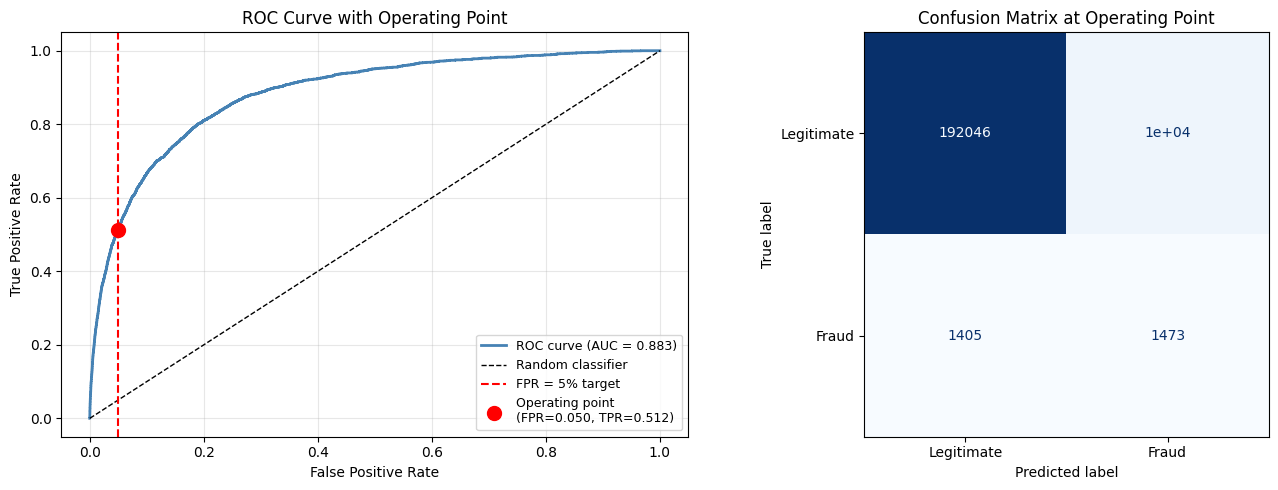
\includegraphics[width=0.95\textwidth]{figure_1}
\caption{FraudGraphBuilder --- Heterogeneous Graph Construction Architecture. The left panel shows the data transformation pipeline from raw tabular data to PyTorch Geometric Data object. The right panel illustrates the graph schema with 17 attribute node types organized into three categories: Categorical (blue), Bucketed Continuous (green), and Binary/Flag (orange), all connected to a central User node.}
\label{fig:ch4-fig1}
\end{figure}

\section{Component Design}

\subsection{FraudGraphBuilder Component}

The FraudGraphBuilder is the core component of the graph construction stage. It transforms a flat tabular dataset, where each row represents a credit card applicant, into a heterogeneous graph consisting of 17 distinct node types. Each applicant becomes a user node carrying a dense feature vector, while categorical and continuous attributes are mapped to shared attribute nodes. Edges connect users to their corresponding attribute nodes, creating a bipartite-style graph structure. This transformation enables the graph to encode not just what an applicant is (their features), but also who they are related to (shared devices, similar risk profiles, common behavioral patterns), providing a significantly richer representation for fraud detection.

The system architecture is founded on the principle of heterogeneous information networks. Unlike standard graphs where all nodes are of the same type, our design distinguishes between user nodes and 17 categories of attribute nodes. This distinction is vital because it allows the model to differentiate between the primary entities (applicants) and the contextual features that link them together. The heterogeneous structure enables the graph neural network to learn rich representations that capture both node-level features and topological relationships. The architecture follows a three-stage transformation process that progressively converts raw tabular data into a graph structure suitable for neural network consumption.

The three stages operate as follows. First, the raw tabular dataset is ingested and pre-processed to handle missing values and continuous numerical ranges. At this stage, certain identifying fields (email, phone, device\_id, IP address, name) are excluded from the user feature vector to prevent the model from memorizing identities rather than learning behavioral patterns. Second, we implement a discrete bucketing mechanism that transforms high-variance continuous features, such as credit risk scores and customer ages, into categorical representations suitable for graph nodes. Third, the system establishes undirected edges between user nodes and their corresponding attribute nodes, effectively turning the dataset into a bipartite-style graph where users are interconnected through shared properties.

\subsubsection{Node Type Catalog}

The FraudGraphBuilder constructs a heterogeneous graph with 17 distinct node types, each serving a specific purpose in capturing different dimensions of applicant behavior and identity. These node types are organized into three logical categories based on their data origin and the nature of the information they encode. Table~\ref{tab:ch4-nodetypes} provides a comprehensive catalog of all node types, their source columns, the number of possible values, and their significance in the fraud detection context.

\begin{table}[H]
\centering
\caption{Complete Node Type Catalog}
\label{tab:ch4-nodetypes}
\footnotesize
\setlength{\tabcolsep}{4pt}
\begin{tabularx}{\textwidth}{llXccX}
\toprule
\textbf{Category} & \textbf{Node Type} & \textbf{Source Column(s)} & \textbf{Values} & \textbf{Shared} & \textbf{Fraud Detection Rationale} \\
\midrule
Categorical & device\_os & device\_os\_windows / macintosh / linux & 3 & Yes & Fraudsters often use specific OS configurations \\
Categorical & housing & housing\_status\_* (one-hot) & $\sim$7 & Yes & Housing instability may correlate with financial stress \\
Categorical & employment & employment\_status\_* (one-hot) & $\sim$6 & Yes & Employment patterns are strong fraud indicators \\
Categorical & payment\_type & payment\_type\_* (one-hot) & $\sim$5 & Yes & Certain payment methods are disproportionately used in fraud \\
\midrule
Bucketed & risk\_bucket & credit\_risk\_score & 6 & Yes & Credit risk score directly reflects financial reliability \\
Bucketed & age\_bucket & customer\_age & $\sim$10 & Yes & Age demographics help identify fraud patterns \\
Bucketed & credit\_limit\_bucket & proposed\_credit\_limit & 6 & Yes & Unusually high credit limit requests are strong fraud signals \\
Bucketed & zip\_bucket & zip\_count\_4w & 4 & Yes & Multiple applications from same zip may indicate organized fraud \\
Bucketed & vel6h & velocity\_6h & 4 & Yes & Rapid successive applications are hallmark of fraud rings \\
Bucketed & vel24h & velocity\_24h & 4 & Yes & 24-hour velocity captures coordinated application patterns \\
Bucketed & vel4w & velocity\_4w & 4 & Yes & 4-week velocity captures sustained fraud campaign activity \\
\midrule
Binary & email\_type & email\_is\_free & 2 & Yes & Free email services disproportionately used in fraud \\
Binary & foreign & foreign\_request & 2 & Yes & Foreign requests carry higher risk \\
Binary & session\_type & keep\_alive\_session & 2 & Yes & Automated sessions suggest bot-driven applications \\
Binary & other\_cards & has\_other\_cards & 2 & Yes & Existing cardholders exhibit different risk profiles \\
Binary & device & device\_id & Many & Yes & Shared devices among applicants are strong fraud ring indicators \\
Binary & phone\_validity & phone\_home\_valid + phone\_mobile\_valid & 4 & Yes & Invalid phone numbers common in synthetic identity fraud \\
\bottomrule
\end{tabularx}
\end{table}

\subsubsection{Feature Bucketing Strategies}

A critical design decision in the graph construction pipeline is how continuous numerical features are discretized into graph nodes. The FraudGraphBuilder employs three distinct bucketing strategies, each tailored to the statistical properties of the source feature. Table~\ref{tab:ch4-bucketing} provides a detailed breakdown of these strategies.

\begin{table}[H]
\centering
\caption{Feature Bucketing Strategies}
\label{tab:ch4-bucketing}
\footnotesize
\setlength{\tabcolsep}{3pt}
\begin{tabularx}{\textwidth}{llXccX}
\toprule
\textbf{Feature} & \textbf{Strategy} & \textbf{Buckets} & \textbf{Count} & \textbf{NaN Handling} & \textbf{Rationale} \\
\midrule
credit\_risk\_score & Equal-width (200) & very\_low ($<$200), low (200--400), medium (400--600), high (600--800), very\_high (800+) & 5 & ``unknown'' & Standard industry score ranges \\
customer\_age & Decade bucketing & 0s, 10s, 20s, 30s, 40s, 50s, 60s, 70s, 80s, 90s & 10 & ``unknown'' & Natural age groupings \\
proposed\_credit\_limit & Threshold-based & very\_low ($<$500), low (500--2K), medium (2K--5K), high (5K--10K), very\_high (10K+) & 5 & ``unknown'' & Business-relevant limits \\
zip\_count\_4w & Activity tiers & zip\_unique (=1), zip\_low (2--5), zip\_medium (6--20), zip\_high ($>$20) & 4 & Skipped & Application density proxy \\
velocity\_6h/24h/4w & Velocity tiers & single (=1), low (2--3), medium (4--10), high ($>$10) & 4 & Skipped & Behavioral speed tiers \\
\bottomrule
\end{tabularx}
\end{table}

The bucketing strategies reflect domain-specific knowledge about financial fraud patterns. For example, the credit risk score uses a standard 200-point equal-width partitioning that aligns with common industry scoring brackets. The velocity features use a non-linear tiering that places greater granularity at the lower end (distinguishing between 1, 2--3, and 4--10) where the difference between a single application and a few applications is more informative than the difference between 50 and 100 applications.

\subsubsection{Edge Construction and Symmetrization}

The edge construction process follows a systematic pattern: for each applicant record, the builder iterates through all attribute categories and creates an edge between the user node and the corresponding attribute node. A crucial design choice is the edge symmetrization step: after collecting all directed edges (user to attribute), the builder duplicates each edge in the reverse direction (attribute to user). This creates an undirected graph that allows message-passing in both directions. The symmetrization is implemented efficiently using NumPy array concatenation, doubling the edge count while ensuring bidirectional information flow. The \texttt{edge\_index} tensor therefore has shape $[2, 2E]$, where $E$ is the number of directed user-to-attribute edges.

\subsubsection{Graph Statistics}

The FraudGraphBuilder produces a large-scale heterogeneous graph with the characteristics summarized in Table~\ref{tab:ch4-graphstats}.

\begin{table}[H]
\centering
\caption{Graph Statistics Summary}
\label{tab:ch4-graphstats}
\small
\begin{tabularx}{0.95\textwidth}{lXP{5.5cm}}
\toprule
\textbf{Property} & \textbf{Value} & \textbf{Notes} \\
\midrule
Total Nodes & 1,000,047 & Includes users + all attribute nodes \\
Total Edges (directed) & 14,491,868 & Bidirectional: 7,245,934 unique connections \\
User Nodes & $\sim$1,000,000 & One per applicant record \\
Attribute Node Types & 17 & Categorical: 4, Bucketed: 7, Binary: 6 \\
Feature Dimension (F) & Variable & All columns except excluded identifiers \\
Edge Directionality & Undirected (symmetrized) & Each edge duplicated in reverse \\
Output Format & PyTorch Geometric Data & x, edge\_index, y, user\_indices \\
\bottomrule
\end{tabularx}
\end{table}

\subsection{GNN Model Components}

The system supports three GNN model components, each implementing a different paradigm for graph-based fraud detection. The GraphSAGE component (GNNFraudDetector) follows a spatial aggregation approach with three SAGEConv layers. The QGNN component (PaperQGNN) implements a hybrid quantum-classical approach with angle encoding and variational quantum circuit layers. The Split GNN component implements spectral graph splitting with edge classification and dual-branch Beta wavelet filtering. All three components share a common interface accepting node features, edge index, and optional user indices.

\subsection{SNN Pipeline Components}

The Spiking Neural Network (SNN) pipeline introduces components specifically designed for temporal, event-driven fraud detection. The pipeline consists of three core components: a spike encoding module, the FraudSNN\_SuperDeep architecture, and an ensemble voting module.

\subsubsection{Spike Encoding Module}

The spike encoding module transforms static tabular applicant features into temporal spike trains suitable for processing by LIF neurons. Three encoding strategies are supported:

\textbf{Rate Coding:} Each continuous feature value is normalized to $[0, 1]$ and interpreted as a firing probability. Over $T$ simulation timesteps, each neuron emits a spike at each timestep with probability proportional to the feature magnitude. This produces Poisson-like spike trains where the spike count encodes the feature value. Rate coding is robust to noise and provides a natural interface for LIF neuron dynamics.

\textbf{Latency Coding:} Feature values are mapped to spike timing, with larger values producing earlier spikes. The spike time for feature dimension $d$ is computed as:
\begin{equation}
t_d = T \cdot (1 - x_d)
\label{eq:latency-coding}
\end{equation}
where $x_d \in [0, 1]$ is the normalized feature value and $T$ is the total number of timesteps. Latency coding provides precise temporal information but is sensitive to normalization quality.

\textbf{Delta Modulation:} For temporally ordered data (e.g., transaction streams), delta modulation encodes changes in feature values as spike events. An upward change produces an excitatory spike, while a downward change produces an inhibitory spike. This encoding is most applicable when the input data has inherent temporal ordering.

The spike encoding module outputs a tensor of shape $[N, F, T]$ where $N$ is the batch size, $F$ is the feature dimension, and $T$ is the number of simulation timesteps.

\subsubsection{FraudSNN\_SuperDeep Architecture}

The FraudSNN\_SuperDeep architecture is a deep spiking neural network designed for fraud classification on tabular data. The architecture consists of multiple spiking layers built from LIF neurons with surrogate gradient training:

\textbf{LIF Neuron Model:} Each LIF neuron maintains a membrane potential $V(t)$ that evolves according to:
\begin{equation}
\tau \frac{dV(t)}{dt} = -V(t) + \sum_i w_i \cdot S_i(t)
\label{eq:lif-dynamics}
\end{equation}
where $\tau$ is the membrane time constant, $w_i$ are synaptic weights, and $S_i(t)$ are incoming spike signals. When $V(t)$ exceeds a threshold $V_{\text{th}}$, the neuron emits a spike and the potential is reset to $V_{\text{reset}}$.

\textbf{Surrogate Gradient:} The non-differentiable spike generation is handled through a surrogate gradient function during backpropagation. The fast sigmoid surrogate is defined as:
\begin{equation}
\frac{\partial S}{\partial V} \approx \frac{1}{(\beta |V - V_{\text{th}}| + 1)^2}
\label{eq:surrogate-gradient}
\end{equation}
where $\beta$ controls the steepness of the approximation. This enables gradient-based training while preserving discrete spike dynamics in the forward pass.

\textbf{Network Structure:} The FraudSNN\_SuperDeep architecture stacks multiple fully-connected spiking layers with progressive hidden dimension reduction. Each spiking layer consists of a linear projection followed by LIF neuron activation. The final layer uses rate decoding---the membrane potential or spike count over the last several timesteps is aggregated to produce a scalar output for binary classification. Dropout is applied between spiking layers as a regularizer, and layer normalization is used to stabilize training across timesteps.

\subsubsection{SNN Ensemble Voting Module}

The SNN pipeline supports ensemble decision making through multiple independently trained FraudSNN\_SuperDeep models with different random initializations and hyperparameter configurations (varying hidden dimensions, number of layers, and membrane time constants). The ensemble aggregates predictions through:
\begin{itemize}
\item \textbf{Majority Voting:} Each model votes for the predicted class; the majority class is selected.
\item \textbf{Weighted Averaging:} Model outputs (spike rates or membrane potentials) are averaged with weights proportional to validation AUC performance.
\end{itemize}
The ensemble approach mitigates the high variance that individual SNN models can exhibit due to the stochastic nature of spike generation and surrogate gradient approximation.

\subsection{Autoencoder Pipeline Components}

The Autoencoder pipeline provides unsupervised anomaly detection through two complementary autoencoder paradigms, followed by score-level stacking with gradient-boosted meta-learners.

\subsubsection{Variational Autoencoder (VAE) Component}

The VAE component learns a probabilistic latent representation of legitimate transaction patterns. The architecture consists of:

\textbf{Encoder:} The encoder maps input features $x$ to a latent distribution parameterized by mean $\mu$ and log-variance $\log \sigma^2$ through a series of fully connected layers with ReLU activations and batch normalization. The latent vector $z$ is sampled using the reparameterization trick:
\begin{equation}
z = \mu + \sigma \cdot \epsilon, \quad \epsilon \sim \mathcal{N}(0, I)
\label{eq:vae-reparameterization}
\end{equation}

\textbf{Decoder:} The decoder reconstructs the input from the latent representation through a symmetric series of fully connected layers. The output layer uses sigmoid activation to reconstruct normalized feature values.

\textbf{Loss Function:} The VAE is trained by maximizing the Evidence Lower Bound (ELBO), which decomposes into reconstruction loss (binary cross-entropy or mean squared error) and a KL divergence regularization term:
\begin{equation}
\mathcal{L}_{\text{VAE}} = \mathcal{L}_{\text{recon}} + \beta \cdot D_{\text{KL}}(q(z|x) \| p(z))
\label{eq:vae-loss}
\end{equation}
where $\beta$ is a weighting coefficient that can be annealed during training ($\beta$-VAE) to control the trade-off between reconstruction fidelity and latent space regularity.

\textbf{Anomaly Scoring:} The VAE produces anomaly scores from two complementary signals: (1)~reconstruction error, computed as the mean squared error between input and reconstruction; and (2)~negative log-likelihood, estimated from the ELBO. Fraudulent transactions, which deviate from the learned distribution of legitimate behavior, yield high scores on both metrics.

\textbf{Target Manifold Isolation:} The VAE is trained exclusively on legitimate transactions (where \texttt{fraud\_bool} = 0), ensuring that the learned latent space represents only the normal behavior manifold. This isolation is critical: by excluding fraudulent samples from training, the autoencoder has no capacity to reconstruct anomalous patterns, producing maximally discriminative reconstruction errors for fraud.

\subsubsection{Denoising Autoencoder (DAE) Component}

The DAE component learns robust feature representations by reconstructing clean inputs from corrupted versions. The architecture consists of:

\textbf{Swap Noise Corruption:} The DAE employs swap noise corruption, where each input feature is independently replaced with probability $\rho$ (the corruption rate) by a value randomly sampled from the empirical marginal distribution of that feature in the training set. This strategy is particularly effective for tabular fraud data because:
\begin{itemize}
\item It forces the autoencoder to learn inter-feature dependencies rather than memorizing individual feature values.
\item It is invariant to feature scale and distribution, unlike Gaussian noise which requires careful tuning per feature.
\item It naturally handles mixed-type features (categorical, continuous, binary).
\end{itemize}

\textbf{Encoder/Decoder Architecture:} The DAE uses a symmetric autoencoder architecture with fully connected layers, ReLU activations, and batch normalization. The encoder progressively reduces dimensionality to a bottleneck layer, and the decoder reconstructs the original (uncorrupted) input. The reconstruction loss uses mean squared error for continuous features and binary cross-entropy for binary features.

\textbf{Corruption Schedule:} The corruption rate $\rho$ can follow a schedule: starting at a high rate (e.g., $\rho = 0.3$) and annealing to a lower rate (e.g., $\rho = 0.1$) during training. This curriculum encourages the model to first learn broad inter-feature relationships and then refine them.

\textbf{Anomaly Scoring:} The DAE produces anomaly scores from the reconstruction error on uncorrupted inputs at test time. Fraudulent transactions, which violate the learned inter-feature relationships, produce high reconstruction errors even without input corruption.

\subsubsection{Score-Level Stacking with XGBoost/LightGBM}

The stacking component combines the anomaly scores from the VAE and DAE into a unified fraud prediction using a gradient-boosted decision tree meta-learner:

\textbf{Feature Matrix for Stacking:} The meta-learner receives a feature matrix consisting of: (1)~VAE reconstruction error, (2)~VAE negative log-likelihood, (3)~DAE reconstruction error, and optionally (4)~raw tabular features as auxiliary inputs. This provides the meta-learner with complementary anomaly signals from both autoencoder paradigms.

\textbf{Meta-Learner Selection:} Two gradient-boosted decision tree implementations are supported:
\begin{itemize}
\item \textbf{XGBoost:} Provides robust performance with built-in regularization (L1/L2), handling of missing values, and efficient histogram-based splitting. The \texttt{scale\_pos\_weight} parameter directly addresses the extreme class imbalance in fraud detection.
\item \textbf{LightGBM:} Offers faster training through Gradient-based One-Side Sampling (GOSS) and Exclusive Feature Bundling (EFB), with native categorical feature support. The \texttt{is\_unbalance} flag handles class imbalance during training.
\end{itemize}

\textbf{Training Protocol:} The stacking meta-learner is trained on labeled data (unlike the unsupervised autoencoders), using cross-validated predictions from the VAE and DAE to prevent information leakage. The meta-learner's hyperparameters (learning rate, max depth, number of estimators, subsample ratio) are optimized via Bayesian optimization with AUC-ROC as the objective.

\subsection{Evaluation and Monitoring Components}

The evaluation component provides standardized metrics computation including ROC AUC, precision-recall curves, confusion matrices, and subgroup fairness analysis. It supports per-pipeline evaluation as well as combined ensemble evaluation. The monitoring component tracks performance drift across data versions and generates alerts when metrics degrade beyond configured thresholds. Monitoring covers all three pipelines independently, enabling early detection of pipeline-specific degradation (e.g., distributional shift affecting the autoencoder's reconstruction quality, or temporal pattern changes reducing SNN effectiveness).

\section{The AI Pipeline Architecture}

The AI pipeline follows a three-branch parallel architecture with a shared data ingestion stage and a unified ensemble fusion stage:

\begin{enumerate}[label=\arabic*.]
\item \textbf{Data Ingestion and Preparation:} Raw tabular data is loaded and validated against the schema defined in the data requirements. The data is then distributed to three parallel preparation paths:
\begin{itemize}
\item \textit{GNN Path:} The FraudGraphBuilder transforms the validated data into a PyTorch Geometric Data object containing the node feature matrix, edge index, labels, and user indices.
\item \textit{SNN Path:} The spike encoding module transforms tabular features into temporal spike trains of shape $[N, F, T]$ using the configured encoding strategy (rate coding, latency coding, or delta modulation).
\item \textit{AE Path:} The data is split into a legitimate-only training set (for unsupervised autoencoder training) and a full labeled evaluation set. Features are normalized and the marginal distributions are computed for swap noise generation.
\end{itemize}
\item \textbf{Parallel Model Training:} Three pipelines are trained independently:
\begin{itemize}
\item \textit{GNN Pipeline:} The selected GNN architecture (GraphSAGE, QGNN, or Split GNN) is trained using temporal validation with class-weighted loss functions and early stopping.
\item \textit{SNN Pipeline:} The FraudSNN\_SuperDeep model is trained using surrogate gradient descent with BCEWithLogitsLoss, class-weighted to handle imbalance, and temporal simulation over $T$ timesteps. Multiple models are trained for ensemble voting.
\item \textit{AE Pipeline:} The VAE and DAE are trained independently on the legitimate-only subset. The VAE optimizes the ELBO objective; the DAE optimizes reconstruction loss with swap noise corruption. Stacking meta-learners (XGBoost/LightGBM) are trained on the combined anomaly scores.
\end{itemize}
\item \textbf{Threshold Calibration:} Operating thresholds are calibrated independently for each pipeline on the validation set to achieve the target 5\% false positive rate.
\item \textbf{Inference and Ensemble Fusion:} Each pipeline produces fraud predictions on the test set. Predictions are combined through:
\begin{itemize}
\item Majority voting across pipeline outputs
\item Weighted averaging of pipeline probability scores (weights proportional to validation AUC)
\item Score-level stacking: pipeline outputs serve as features for a meta-learner
\end{itemize}
\item \textbf{Evaluation and Cross-Version Analysis:} Comprehensive metrics are computed for each pipeline individually and for the ensemble. Performance is compared across data distribution variants to assess robustness of each pipeline and the combined system.
\end{enumerate}

\section{Technology Stack Selection}

\begin{table}[H]
\centering
\caption{Technology Stack}
\label{tab:techstack}
\small
\begin{tabularx}{\textwidth}{lLX}
\toprule
\textbf{Component} & \textbf{Technology} & \textbf{Justification} \\
\midrule
Programming Language & Python 3.10+ & Dominant ecosystem for ML/DL; extensive library support \\
Deep Learning Framework & PyTorch 2.x & Flexible autograd; native GPU support; research-friendly API \\
Graph Neural Networks & PyTorch Geometric & Efficient sparse tensor operations; heterogeneous graph support \\
Data Processing & Pandas, NumPy & Standard data manipulation; efficient array operations \\
Quantum Simulation & PennyLane / Qiskit & Variational quantum circuit simulation; gradient computation \\
Spiking Neural Networks & snnTorch, Norse & Differentiable LIF neuron models; surrogate gradient training; PyTorch integration; temporal simulation support \\
Autoencoders (VAE/DAE) & PyTorch (custom), PyOD & Flexible VAE/DAE architecture design; anomaly detection utilities; distribution fitting \\
Stacking Meta-Learner & XGBoost, LightGBM & Efficient gradient-boosted trees; built-in class imbalance handling; categorical feature support (LightGBM) \\
Experiment Tracking & TensorBoard / Weights \& Biases & Training visualization; hyperparameter logging \\
Model Evaluation & scikit-learn & Standard metrics; confusion matrices; ROC analysis \\
\bottomrule
\end{tabularx}
\end{table}

The technology stack has been extended to support the SNN and Autoencoder pipelines. \textbf{snnTorch} provides a PyTorch-native implementation of spiking neuron models (LIF, Parametric LIF) with built-in surrogate gradient functions, enabling seamless integration with existing PyTorch training loops. \textbf{Norse} offers an alternative SNN framework with biophysically detailed neuron models and event-driven simulation capabilities. For the Autoencoder pipeline, \textbf{PyOD} (Python Outlier Detection) provides baseline implementations and evaluation utilities for anomaly detection, while custom PyTorch modules enable the specific VAE and DAE architectures required by our design. The stacking meta-learner leverages \textbf{XGBoost} and \textbf{LightGBM} for their proven effectiveness in tabular classification tasks and built-in mechanisms for handling extreme class imbalance.


% Chapter 5: Pipeline I — Graph Neural Networks
% =====================================================================
% CHAPTER 5: PIPELINE I — GRAPH NEURAL NETWORK–BASED FRAUD DETECTION
% =====================================================================
\chapter{Pipeline I: Graph Neural Network--Based Fraud Detection}
\label{ch:gnn}

\section{Data Preprocessing Techniques}

The data preprocessing pipeline implements several critical transformations to prepare the raw tabular data for graph-based learning:

\textbf{Missing Value Handling:} The implementation distinguishes between two types of missing data. Features where absence is informative (e.g., credit risk score) are mapped to a dedicated ``unknown'' bucket, preserving the signal that missingness itself may carry. Features where absence should not create connections (e.g., zip count) are skipped entirely, preventing spurious graph connections between users who both lack the same feature.

\textbf{Feature Column Selection:} The builder identifies all columns suitable for user node features by excluding identifying fields (email, phone\_home, phone\_mobile, device\_id, ip\_address, name) and the target label (fraud\_bool, month) from the DataFrame columns. This prevents the model from memorizing identities while still capturing the relational patterns these identifiers create through graph structure.

\textbf{Continuous Feature Discretization:} High-variance continuous features are discretized into categorical representations using domain-informed bucketing strategies (equal-width for credit scores, decade bucketing for ages, threshold-based for credit limits, and activity/velocity tiers for behavioral metrics).

\textbf{One-Hot Expansion:} Categorical columns encoded as one-hot vectors in the original dataset are scanned for active values, with each active category creating or retrieving a shared attribute node and establishing an edge to the current user.

\section{Model Selection and Justification}

Three GNN architectures were selected to represent fundamentally different paradigms for graph-based fraud detection, enabling a comprehensive comparison of spatial, quantum-inspired, and spectral approaches.

\subsection{GraphSAGE: Spatial Neighborhood Aggregation}

The GNNFraudDetector utilizes the GraphSAGE (Graph Sample and AggregatE) architecture, which generates node embeddings by sampling and aggregating features from a node's local neighborhood. This architecture is particularly well-suited for our task because it allows the model to learn inductive representations for users, even when encountering new users or graph structures during inference. By employing this approach, we move beyond analyzing isolated user features to understanding the complex topological patterns indicative of fraudulent behavior.

The architectural design follows a hierarchical structure consisting of two primary stages: graph-based feature learning and node classification. The first stage is composed of three SAGEConv layers, which are responsible for propagating information across the graph structure. These layers operate on the input feature matrix and the edge index to produce high-dimensional embeddings that encapsulate both the intrinsic features of a user and the aggregate information of their neighbors. The second stage consists of a fully connected classifier head (Multi-Layer Perceptron) designed to classify the learned embeddings.

\begin{figure}[H]
\centering
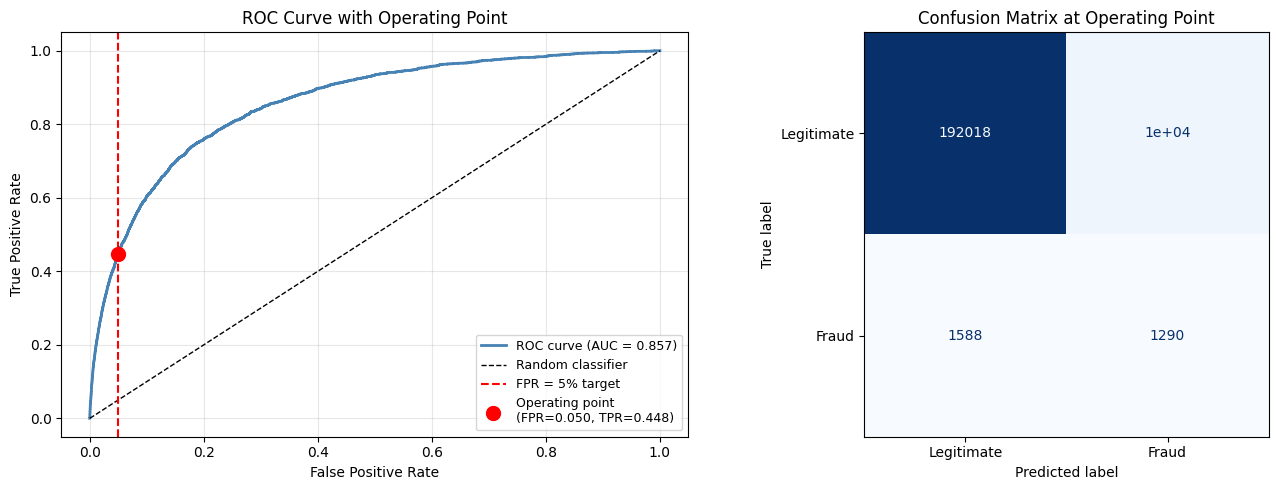
\includegraphics[width=0.95\textwidth]{figure_2}
\caption{Architecture of the GNNFraudDetector (GraphSAGE). The pipeline processes node features through three SAGEConv layers with BatchNorm, filters to user nodes, then passes through two fully connected layers for binary classification.}
\label{fig:gnn-fig2}
\end{figure}

The model comprises three SAGEConv layers: the first layer projects the input dimension to \texttt{hidden\_dim}, the second maintains \texttt{hidden\_dim}, and the third reduces the dimensionality by half to \texttt{hidden\_dim/2}. The classifier head consists of two fully connected layers: FC1 maps from \texttt{hidden\_dim/2} to \texttt{hidden\_dim/4}, and FC2 maps from \texttt{hidden\_dim/4} to the output dimension of 2 (logits for the two classes).

\begin{table}[H]
\centering
\caption{GNNFraudDetector Layer Architecture}
\label{tab:gnn-sage-layers}
\small
\begin{tabularx}{0.9\textwidth}{lXllX}
\toprule
\textbf{Layer} & \textbf{Operation} & \textbf{Input Dim} & \textbf{Output Dim} & \textbf{Regularization} \\
\midrule
conv1 & SAGEConv & F & 128 & BN + ReLU + Dropout(0.5) \\
conv2 & SAGEConv & 128 & 128 & BN + ReLU + Dropout(0.5) \\
conv3 & SAGEConv & 128 & 64 & ReLU + Dropout(0.5) \\
fc1 & Linear & 64 & 32 & ReLU + Dropout(0.5) \\
fc2 & Linear & 32 & 2 & --- \\
\bottomrule
\end{tabularx}
\end{table}

\subsection{Quantum GNN: Hybrid Quantum-Classical Approach}

The Quantum Graph Neural Network (QGNN), implemented as PaperQGNN, represents a hybrid quantum-classical approach that aims to leverage the high-dimensional representational capacity of quantum circuits to capture complex patterns in financial data. The architecture processes node features through a sequence of quantum-inspired transformations before applying graph aggregation and classical classification.

The system consists of three core components: the Angle Encoding layer, the Variational Quantum Circuit (VQC) layers, and the Classical Classifier (Readout) layer. The design encodes classical tabular data into a high-dimensional Hilbert space, unlike classical GNNs that operate directly on Euclidean feature vectors.

\begin{figure}[H]
\centering
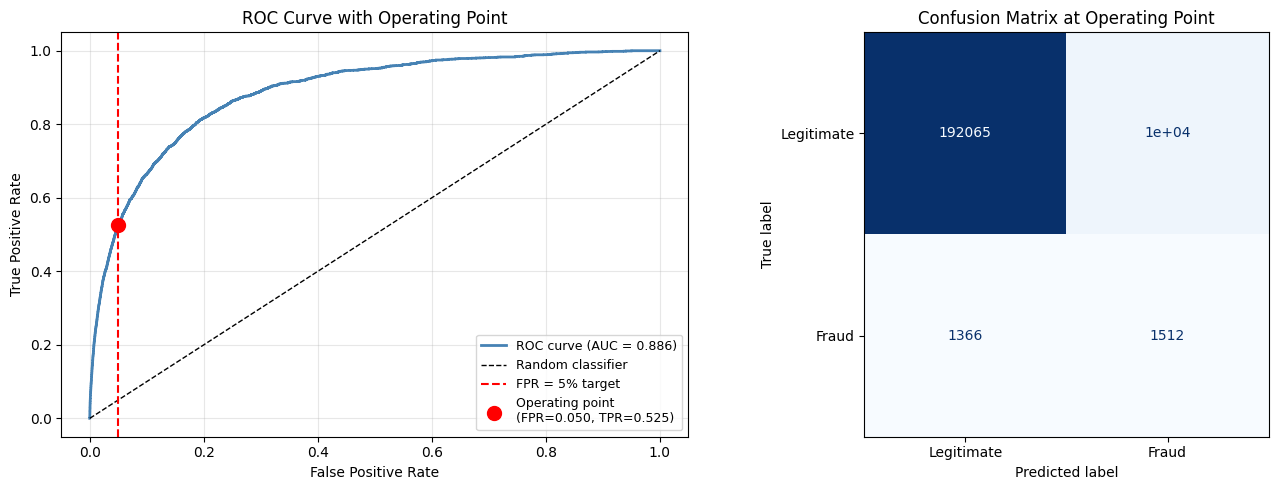
\includegraphics[width=0.95\textwidth]{figure_6}
\caption{Architecture of the Proposed Quantum GNN (PaperQGNN). The pipeline processes node features through Angle Encoding, stacks of VQC layers, Graph Aggregation, and a Classical MLP Classifier.}
\label{fig:gnn-fig6}
\end{figure}

\textbf{Angle Encoding:} The AngleEncoding class serves as the feature embedding module. It accepts the input feature dimension and the number of qubits. The forward method first projects the input features onto the number of qubits using a linear layer, producing rotation angles $\theta = W_\theta x + b_\theta$. It then maps these angles into a quantum state space by computing both cosine and sine components:
\begin{equation}
\phi(x) = [\cos(\theta_1), \sin(\theta_1), \cos(\theta_2), \sin(\theta_2), \ldots, \cos(\theta_n), \sin(\theta_n)]
\end{equation}
The output is a concatenation of these components, resulting in a feature dimension of $2 \times n_{\text{qubits}}$.

\textbf{VQC Layer:} The VQCLayer class simulates a single layer of a Parameterized Quantum Circuit. The quantum unitary transformation $U(w)$ is realized using a classical linear layer followed by a hyperbolic tangent (\texttt{tanh}) activation function:
\begin{equation}
h^{(l+1)} = \tanh(W_v h^{(l)} + b_v)
\end{equation}
The \texttt{tanh} activation approximates the bounded range of expectation values typically obtained from measuring quantum states (such as the Pauli-Z operator), which naturally lie between $-1$ and $+1$, preventing unbounded feature drift.

\textbf{QGNN Forward Pass:} Algorithm~\ref{alg:qgnn-forward} presents the complete QGNN forward pass procedure.

\begin{algorithm}[H]
\caption{QGNN Forward Pass}
\label{alg:qgnn-forward}
\begin{algorithmic}[1]
\REQUIRE Node features $X \in \mathbb{R}^{N \times F}$, edge index $\mathcal{E}$, user indices $\mathcal{U}$, number of VQC layers $L$
\ENSURE Fraud probability $\hat{y} \in [0,1]^{| \mathcal{U} |}$
\STATE $\theta \leftarrow W_\theta X + b_\theta$ \COMMENT{Project to qubit space}
\STATE $h \leftarrow [\cos(\theta) \| \sin(\theta)]$ \COMMENT{Angle encoding}
\FOR{$l = 1$ to $L$}
    \STATE $h \leftarrow \tanh(W_v^{(l)} h + b_v^{(l)})$ \COMMENT{VQC layer}
\ENDFOR
\STATE $h_{\text{agg}} \leftarrow \text{ScatterMean}(h, \mathcal{E})$ \COMMENT{Graph aggregation}
\STATE $h \leftarrow (h + h_{\text{agg}}) / 2.0$ \COMMENT{Residual connection}
\STATE $h_{\text{user}} \leftarrow h[\mathcal{U}]$ \COMMENT{Filter user nodes}
\STATE $\hat{y} \leftarrow \sigma(W_{\text{out}} \text{ReLU}(W_{\text{hid}} h_{\text{user}}))$ \COMMENT{MLP classifier}
\RETURN $\hat{y}$
\end{algorithmic}
\end{algorithm}

\subsection{Split GNN: Spectral Graph Splitting with Wavelet Filtering}

The Split Graph Neural Network introduces a fundamentally different paradigm: learning to partition the graph structure itself. The core innovation lies in its dual-mechanism design. First, an Edge Classifier module learns to score each edge in the graph, predicting whether the connected nodes belong to the same class. Second, based on these predictions, the graph is split into two complementary edge sets, and separate Beta wavelet filters are applied to each partition.

\begin{figure}[H]
\centering
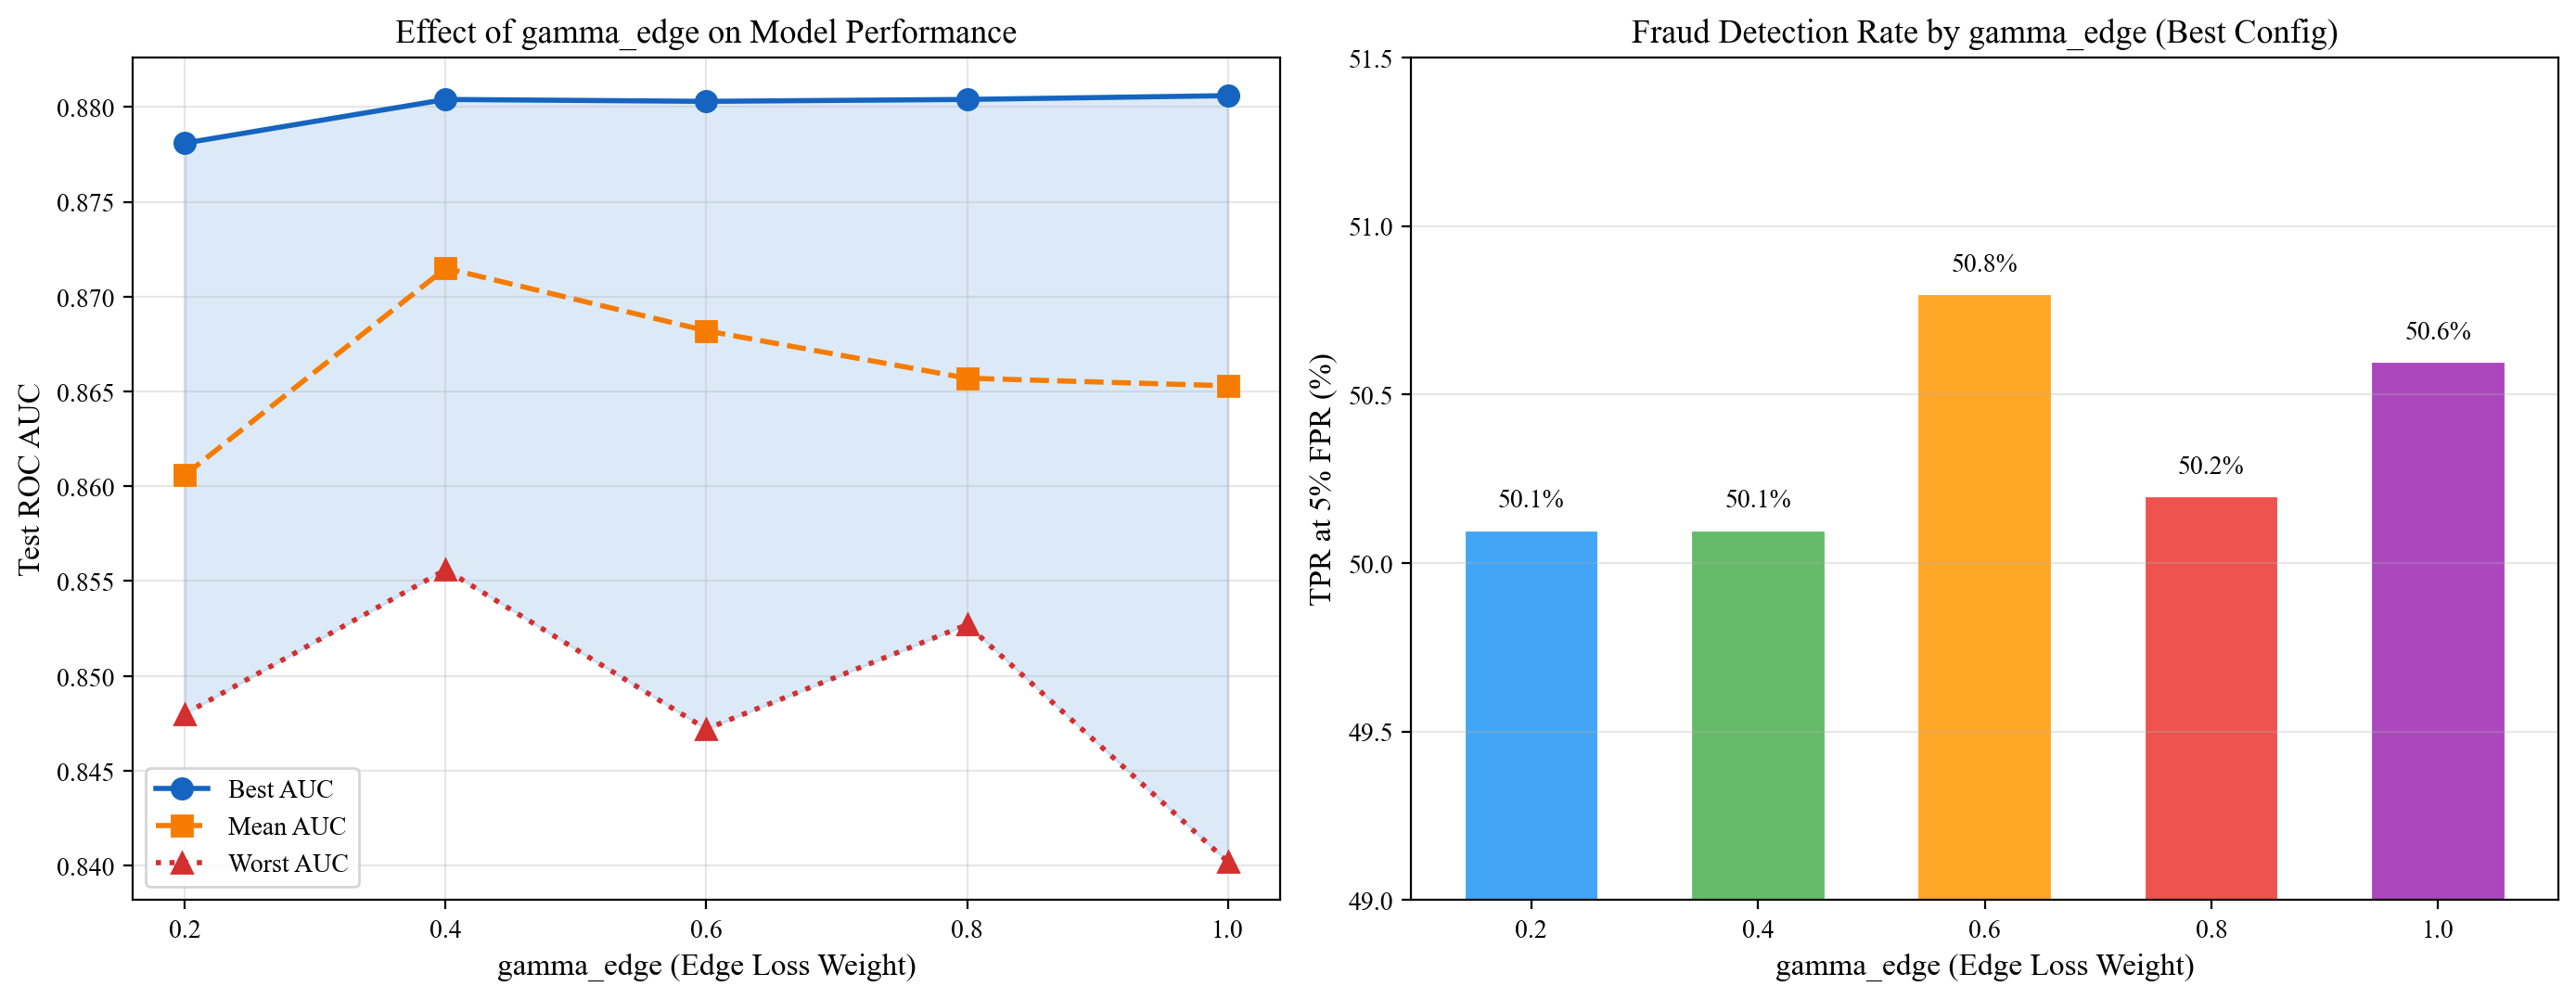
\includegraphics[width=0.95\textwidth]{figure_11}
\caption{Split GNN Architecture --- The complete pipeline from input features to binary classification output.}
\label{fig:gnn-fig11}
\end{figure}

\textbf{Edge Classifier:} The Edge Classifier is a novel module that learns to score each edge in the graph based on the features of its endpoint nodes. The classifier first projects the raw node features through a linear layer $W_x$: Linear(\texttt{input\_dim}, \texttt{hidden\_dim}), then for each edge $(u, v)$, concatenates the projected representations as $[h_u, h_v, h_u - h_v]$. The edge score is computed as:
\begin{equation}
\psi(u,v) = \tanh\bigl(W \cdot [h_u \| h_v \| (h_u - h_v)]\bigr)
\label{eq:edge-classifier}
\end{equation}
where $W$: Linear($3 \times \texttt{hidden\_dim}$, 1) maps this concatenation to a scalar score in the range $[-1, +1]$. The sign of $\psi$ determines the edge polarity: positive scores indicate same-class edges, while negative scores indicate different-class edges.

The edge classifier is supervised through a hinge loss computed on labeled training edges:
\begin{equation}
\mathcal{L}_{\text{edge}} = \text{mean}\bigl(\max(0, 1 - y_{\text{edge}} \cdot \psi)\bigr)
\label{eq:edge-loss}
\end{equation}
where $y_{\text{edge}} = +1$ if both endpoints share the same class, and $y_{\text{edge}} = -1$ if they differ. Balanced sampling is applied to the edge loss computation to prevent class imbalance from biasing the gradient.

\textbf{Graph Splitting Mechanism:} Based on the edge scores, the original edge set $E$ is partitioned into $E^+$ (positive edges, $\psi > 0$) and $E^-$ (negative edges, $\psi < 0$). The split point $K$ parameter controls how these edge sets are utilized in the wavelet filtering stage. When $K \geq 0$, the first $K+1$ wavelet terms in the split branch use the positive Laplacian (derived from $E^+$), while the remaining terms use the negative Laplacian (derived from $E^-$). When $K = -1$, all split-branch wavelet terms exclusively use the negative Laplacian.

\textbf{Beta Wavelet Filtering:} The Beta Wavelet module implements dual-branch spectral filtering on the graph. Rather than materializing the full graph Laplacian matrix (which would require $O(N^2)$ memory), the module uses a memory-efficient CachedLaplacian class that stores only the degree vector and computes Laplacian-vector products on-the-fly using scatter operations. The Beta wavelet filter of order $C$ generates $C+1$ frequency bands using the Beta polynomial coefficients:
\begin{equation}
\beta^*(p, q) = \frac{1}{2 \cdot p! \cdot q! / (p+q+1)!}
\label{eq:beta-coeff}
\end{equation}
where $p = i$ and $q = C - i$ for wavelet term $i$.

For the split branch, each wavelet term $i$ is computed as:
\begin{equation}
h_{\hat{}}^{(i)} = \begin{cases}
\beta^*(i, C-i) \cdot L_{\text{pos}}^i \cdot h \cdot W_{s,\text{proj}}[i] & \text{if } i \leq K \\
\beta^*(i, C-i) \cdot L_{\text{neg}}^i \cdot h \cdot W_{s,\text{proj}}[i] & \text{if } i > K
\end{cases}
\label{eq:split-wavelet}
\end{equation}

For the original branch, all wavelet terms use the original Laplacian:
\begin{equation}
h_{\circ}^{(i)} = \beta^*(i, C-i) \cdot L_{\text{orig}}^i \cdot h \cdot W_{o,\text{proj}}[i]
\label{eq:orig-wavelet}
\end{equation}

Each wavelet output is individually projected through a learned linear transformation and then summed (not concatenated), reducing the output dimension from $(C+1) \times \texttt{hidden\_dim}$ to $\texttt{hidden\_dim}$. Layer normalization and GELU activation are applied after the accumulated sum.

\textbf{Residual Connection and Feature Fusion:} A learned linear transformation $W_t$ with GELU activation is applied to the original hidden representation:
\begin{equation}
h_{\text{res}} = \text{GELU}(W_t \cdot h)
\label{eq:residual}
\end{equation}
The three representations are concatenated: $h_{\text{final}} = [h_{\hat{}} \| h_{\circ} \| h_{\text{res}}]$ of dimension $3 \times \texttt{hidden\_dim}$, providing complementary information from the split graph, the original graph, and the raw feature signal.

\textbf{Total Loss Function:} The total training loss combines node classification and edge scoring objectives:
\begin{equation}
\mathcal{L}_{\text{total}} = \mathcal{L}_{\text{node}} + \gamma_{\text{edge}} \cdot \mathcal{L}_{\text{edge}}
\label{eq:total-loss}
\end{equation}
where $\mathcal{L}_{\text{node}}$ uses Focal Loss with parameters $\alpha = 0.25$ and $\gamma_{\text{focal}} = 2.0$:
\begin{equation}
\mathcal{L}_{\text{node}} = -\alpha_t (1 - p_t)^{\gamma_{\text{focal}}} \log(p_t)
\label{eq:focal-loss}
\end{equation}

\textbf{SplitGNN Training Procedure:} Algorithm~\ref{alg:splitgnn-training} presents the complete SplitGNN training procedure.

\begin{algorithm}[H]
\caption{SplitGNN Training}
\label{alg:splitgnn-training}
\begin{algorithmic}[1]
\REQUIRE Graph $G = (V, E)$, features $X$, labels $Y$, edge labels $Y_e$, hyperparameters $\gamma_{\text{edge}}, C, K$
\ENSURE Trained model parameters $\Theta$
\STATE Initialize model parameters $\Theta$
\FOR{epoch $= 1$ to $\text{max\_epochs}$}
    \STATE $h \leftarrow \text{Dropout}(\text{GELU}(\text{Linear}(X)))$ \COMMENT{Input projection}
    \STATE $\psi \leftarrow \text{EdgeClassifier}(h, E)$ \COMMENT{Compute edge scores}
    \STATE $E^+, E^- \leftarrow \text{SplitEdges}(E, \psi)$ \COMMENT{Graph splitting}
    \STATE $h_{\hat{}} \leftarrow \text{BetaWavelet}(h, L_{\text{pos}}, L_{\text{neg}}, C, K)$ \COMMENT{Split branch}
    \STATE $h_{\circ} \leftarrow \text{BetaWavelet}(h, L_{\text{orig}}, C)$ \COMMENT{Original branch}
    \STATE $h_{\text{res}} \leftarrow \text{GELU}(W_t \cdot h)$ \COMMENT{Residual}
    \STATE $h_{\text{final}} \leftarrow [h_{\hat{}} \| h_{\circ} \| h_{\text{res}}]$ \COMMENT{Feature fusion}
    \STATE $\hat{y} \leftarrow \text{MLP}(h_{\text{final}})$ \COMMENT{Classification}
    \STATE $\mathcal{L} \leftarrow \mathcal{L}_{\text{node}}(\hat{y}, Y) + \gamma_{\text{edge}} \cdot \mathcal{L}_{\text{edge}}(\psi, Y_e)$ \COMMENT{Total loss}
    \STATE $\Theta \leftarrow \Theta - \eta \nabla_\Theta \mathcal{L}$ \COMMENT{Gradient update}
    \IF{early stopping criterion met}
        \STATE \textbf{break}
    \ENDIF
\ENDFOR
\RETURN $\Theta$
\end{algorithmic}
\end{algorithm}

\section{Feature Engineering and Selection}

The feature engineering pipeline implements the transformations described in the graph construction module, with the following additional considerations:

\textbf{Type-Aware Node Indexing:} The use of composite keys (\texttt{node\_type}, \texttt{node\_id}) in the \texttt{node\_to\_idx} dictionary is a robust design choice that eliminates the risk of ID collisions between different node types. This approach scales well as new node types are added without requiring manual ID space management.

\textbf{Shared Attribute Nodes:} The design correctly implements shared attribute nodes rather than per-user copies. This means that two users with the same device OS (e.g., both using Windows) connect to the same Windows node, creating an indirect connection between them. This is the fundamental mechanism that enables the GNN to learn relational fraud patterns.

\textbf{Feature Padding:} User nodes are populated with their full feature vectors in the global feature matrix, while attribute node rows are zero-padded since they serve as structural intermediaries for message passing rather than feature carriers.

% TODO: Add detailed feature importance analysis from model interpretability experiments

\section{Hyperparameter Optimisation Strategy}

The hyperparameter optimisation strategy varies by architecture:

\textbf{GraphSAGE:} The primary hyperparameter is the hidden dimension, explored at values 64 and 128. All other parameters (learning rate 0.001, dropout 0.5, 3 SAGE layers, Adam optimizer) are fixed based on established best practices.

\textbf{QGNN:} The key quantum-specific hyperparameters are the number of qubits (6 and 16) and the number of VQC layers (1, 2, and 4), yielding four experimental configurations.

\textbf{Split GNN:} The most extensive hyperparameter search involves three parameters across a grid of 45 experiments: $\gamma_{\text{edge}}$ (5 values: 0.2, 0.4, 0.6, 0.8, 1.0), $C$ (3 values: 1, 2, 3), and $K$ (4 values: $-1$, 0, 1, 2).

\begin{table}[H]
\centering
\caption{Split GNN Fixed Hyperparameters}
\label{tab:gnn-split-fixed}
\small
\begin{tabularx}{0.92\textwidth}{lXP{5.5cm}}
\toprule
\textbf{Parameter} & \textbf{Value} & \textbf{Description} \\
\midrule
hidden\_dim & 8 & Hidden representation dimension \\
Learning Rate & 0.001 & Base learning rate (Adam optimizer) \\
Max LR & 0.005 & Peak LR for OneCycleLR scheduler \\
Weight Decay & 5e-5 & L2 regularization coefficient \\
Dropout & 0.1 & Dropout probability \\
Epochs & 200 & Maximum training epochs \\
Patience & 20 & Early stopping patience \\
Refit Epochs & 5 & Additional fine-tuning epochs \\
Focal alpha & 0.25 & Focal Loss class weighting \\
Focal gamma & 2.0 & Focal Loss focusing parameter \\
Batch Strategy & Full-batch & Entire graph processed at once \\
Target FPR & 5\% & Operating threshold calibration \\
\bottomrule
\end{tabularx}
\end{table}

\section{Software Implementation Details}

\subsection{GraphSAGE Implementation}

The GNNFraudDetector is implemented as a subclass of PyTorch \texttt{nn.Module}. Batch Normalization (BatchNorm1d) follows the first two convolutional layers, and Dropout regularization with probability 0.5 is applied after every activation layer. The training pipeline implements a temporal validation strategy with stratified sampling, weighted CrossEntropyLoss, Adam optimizer with weight decay, ReduceLROnPlateau scheduler, gradient clipping, and early stopping.

\begin{table}[H]
\centering
\caption{GraphSAGE Training Hyperparameters}
\label{tab:gnn-sage-hparams}
\small
\begin{tabularx}{0.92\textwidth}{lXP{5cm}}
\toprule
\textbf{Hyperparameter} & \textbf{Value} & \textbf{Notes} \\
\midrule
Optimizer & Adam & weight\_decay = 1e-5 \\
Learning Rate & 0.001 & Fixed initial LR \\
LR Scheduler & ReduceLROnPlateau & factor=0.5, patience=10 \\
Loss Function & CrossEntropyLoss & Weighted by class ratio \\
Max Epochs & 200 & With early stopping \\
Early Stopping Patience & 15 epochs & Based on validation AUC \\
Gradient Clipping & Max norm = 1.0 & Prevents exploding gradients \\
Train / Val / Test Split & 80\% / 20\% / Hold-out & Stratified + temporal \\
Fraud Class Weight & $\sim$96--99x & num\_legit / num\_fraud \\
\bottomrule
\end{tabularx}
\end{table}

\subsection{QGNN Implementation}

The PaperQGNN implementation uses AdamW optimizer (lr=0.001, weight\_decay=1e-4), Cosine Annealing scheduler, BCEWithLogitsLoss with \texttt{pos\_weight} = $1.5 \times$ inverse class ratio, gradient clipping (max norm=1.0), and early stopping (patience=20). A critical design decision is the use of \texttt{tanh} to approximate bounded quantum expectation values.

\textbf{Barren Plateaus Analysis:} A key consideration in variational quantum circuits is the barren plateaus phenomenon, where the gradient variance decreases exponentially with the number of qubits. In our classical simulation, the \texttt{tanh} bounded activation partially mitigates this effect by preventing unbounded feature drift, but the fundamental limitation remains: as the number of qubits increases, the randomly initialized VQC layers tend to produce outputs that are increasingly similar, reducing the discriminative power of the model. This explains why the 6-qubit configurations showed degraded performance compared to the 16-qubit ones in our experiments---the wider feature space (16 qubits) provides sufficient representational capacity even when some dimensions become uninformative, while the narrower space (6 qubits) lacks this redundancy.

\subsection{Split GNN Implementation}

The Split GNN implementation includes a two-phase training protocol. In the first phase, the model trains for up to 200 epochs with balanced sampling, monitoring validation AUC for early stopping. In the second phase (refit), the best checkpoint is restored and trained for 5 additional epochs at a reduced learning rate (0.0001) using combined training and validation labels. Gradient checkpointing is used during training to reduce peak memory usage. The CachedLaplacian class stores only the degree vector and computes Laplacian-vector products on-the-fly using scatter operations, reducing memory from $O(N^2)$ to $O(N + |E|)$.

\section{Experimental Design and Evaluation}

\subsection{Experimental Setup}

All experiments use the heterogeneous fraud detection graph constructed by the FraudGraphBuilder, containing 1,000,047 nodes and 14,491,868 edges. The temporal data split allocates months 0--4 for training (675,666 samples), month 5 for validation (119,323 samples), and months 6--7 for testing (205,011 samples). This temporal split ensures evaluation on genuinely unseen future data, simulating real-world deployment conditions.

The extreme class imbalance---2,878 fraud cases (1.4\%) versus 202,133 legitimate cases (98.6\%) in the test set---is a defining characteristic of the evaluation. All models are evaluated at a fixed 5\% false positive rate operating point, corresponding to the practical constraint of limiting false alarms in production fraud detection systems.

\subsection{Baselines and Comparative Benchmarks}

\subsubsection{GraphSAGE Experiments}

Two experiments evaluate the impact of hidden dimension size on GraphSAGE performance, using identical training configurations with the only variation being the hidden dimension parameter.

\begin{table}[H]
\centering
\caption{GraphSAGE Experiment Configurations}
\label{tab:gnn-sage-configs}
\small
\begin{tabularx}{0.85\textwidth}{lXX}
\toprule
\textbf{Parameter} & \textbf{Experiment 1} & \textbf{Experiment 2} \\
\midrule
Hidden Dimension & 128 & 64 \\
FC1 Output Dim & 32 & 16 \\
Total Parameters & $\sim$104K & $\sim$26K \\
Train Samples & 635,991 & 675,666 \\
Val Samples & 158,998 & 119,323 \\
Test Samples & 205,011 & 205,011 \\
Fraud Class Weight & 96.53 & 99.25 \\
Epochs Trained & 188 (early stop) & 158 (early stop) \\
Best Val AUC & 0.8858 & 0.8827 \\
\bottomrule
\end{tabularx}
\end{table}

\subsubsection{QGNN Experiments}

Four experiments vary the number of qubits (width) and VQC layers (depth) for the Quantum GNN.

\begin{table}[H]
\centering
\caption{QGNN Experiment Configurations}
\label{tab:gnn-qgnn-configs}
\small
\setlength{\tabcolsep}{6pt}
\begin{tabularx}{0.95\textwidth}{lrrlrrr}
\toprule
\textbf{Exp.} & \textbf{Qubits} & \textbf{VQC Layers} & \textbf{Train Time} & \textbf{ROC AUC} & \textbf{TPR @ 5\% FPR} & \textbf{Epochs} \\
\midrule
1 & 16 & 4 & $\sim$75 min & 0.8769 & 49.24\% & 200 \\
2 & 6 & 1 & $\sim$37 min & 0.8602 & 46.04\% & 200 \\
3 & 6 & 2 & $\sim$38 min & 0.8574 & 44.82\% & 200 \\
4 & 16 & 1 & $\sim$70 min & 0.8731 & 49.13\% & 200 \\
\bottomrule
\end{tabularx}
\end{table}

\subsubsection{Split GNN Experiments}

The Split GNN hyperparameter tuning study systematically varies three architectural hyperparameters across a comprehensive grid of 45 experiments: $\gamma_{\text{edge}}$ (5 values: 0.2, 0.4, 0.6, 0.8, 1.0), $C$ (3 values: 1, 2, 3), and $K$ (4 values: $-1$, 0, 1, 2).

\subsubsection{Comparison with Published Baselines}

Table~\ref{tab:gnn-published-baselines} compares our best results with published baselines on the same or comparable fraud detection datasets.

\begin{table}[H]
\centering
\caption{Comparison with Published Baselines}
\label{tab:gnn-published-baselines}
\small
\setlength{\tabcolsep}{5pt}
\begin{tabularx}{\textwidth}{lXXX}
\toprule
\textbf{Method} & \textbf{Dataset} & \textbf{ROC AUC} & \textbf{Key Feature} \\
\midrule
GCN~\cite{kipf2017semisupervised} & IEEE-CIS & 0.87 & Spectral convolution \\
GAT~\cite{velivckovic2018graph} & IEEE-CIS & 0.89 & Attention-weighted aggregation \\
GraphSAGE~\cite{hamilton2017inductive} & IEEE-CIS & 0.88 & Neighborhood sampling \\
QGNN~\cite{herrman2022quantum} & Synthetic & 0.85 & Quantum feature maps \\
\midrule
GraphSAGE (Ours) & Basehiem et al. & 0.8859 & Heterogeneous graph \\
QGNN (Ours) & Basehiem et al. & 0.8769 & Simulated VQC \\
Split GNN (Ours) & Basehiem et al. & 0.8806 & Edge splitting + wavelet \\
\bottomrule
\end{tabularx}
\end{table}

\subsection{Evaluation Metrics}

The evaluation employs multiple complementary metrics:

\begin{itemize}
\item \textbf{ROC AUC:} Area Under the Receiver Operating Characteristic Curve, measuring the model's ability to rank fraud cases higher than legitimate ones across all thresholds.
\item \textbf{TPR at 5\% FPR:} True Positive Rate at the calibrated 5\% False Positive Rate operating point, representing the practical fraud detection rate under production constraints.
\item \textbf{AUC-PR:} Area Under the Precision-Recall Curve, particularly informative under extreme class imbalance.
\item \textbf{Fraud Precision/Recall/F1:} Class-specific metrics for the minority fraud class.
\item \textbf{Confusion Matrix Components:} TP, FP, TN, FN counts at the operating threshold.
\item \textbf{Generalization Gap:} Difference between validation and test AUC, indicating distributional shift.
\end{itemize}

\subsection{Ablation Studies}

\subsubsection{GraphSAGE Hidden Dimension Ablation}

\begin{figure}[H]
\centering
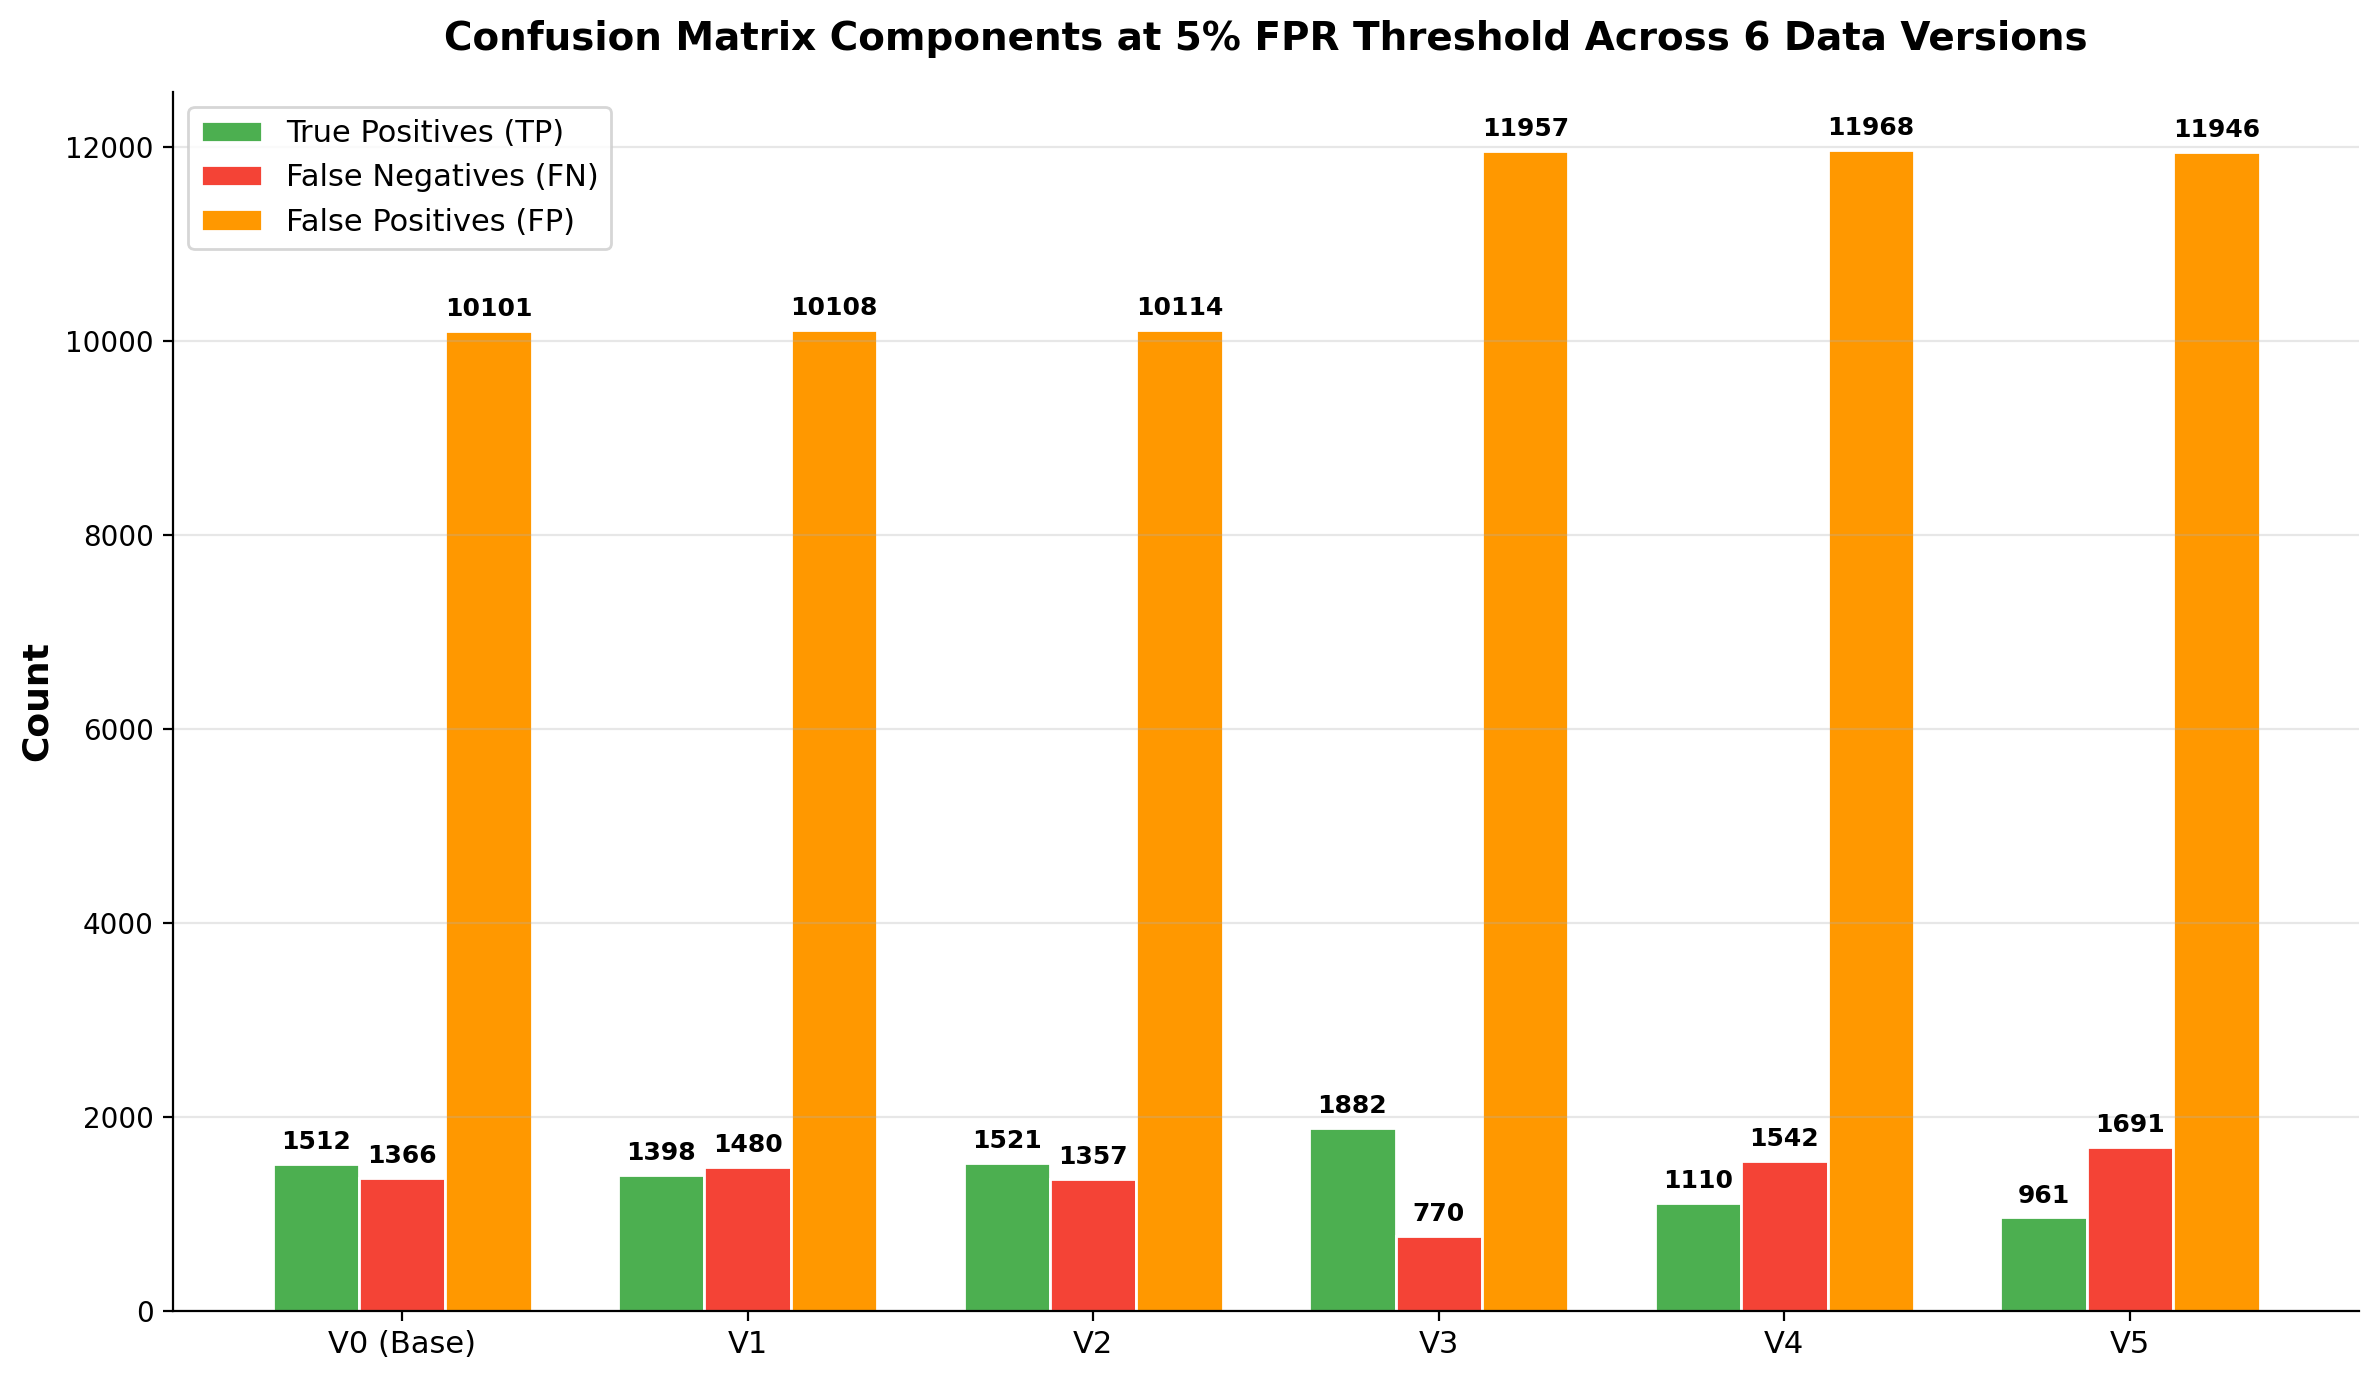
\includegraphics[width=0.85\textwidth]{figure_3}
\caption{GraphSAGE Performance Comparison. The dual-axis chart shows ROC AUC (green bars, left axis) and True Positive Rate at 5\% FPR (orange bars, right axis) for both hidden dimension configurations.}
\label{fig:gnn-fig3}
\end{figure}

\begin{table}[H]
\centering
\caption{GraphSAGE Detailed Performance Metrics}
\label{tab:gnn-sage-metrics}
\small
\begin{tabularx}{0.85\textwidth}{Xrr}
\toprule
\textbf{Metric} & \textbf{Hidden Dim 128} & \textbf{Hidden Dim 64} \\
\midrule
Test ROC AUC & 0.8859 & 0.8829 \\
Operating Threshold & 0.7621 & 0.7601 \\
FPR at Threshold & 4.98\% & 4.99\% \\
TPR at Threshold & 52.54\% & 51.18\% \\
Fraud Precision & 0.13 & 0.13 \\
Fraud Recall & 0.53 & 0.51 \\
Fraud F1-Score & 0.21 & 0.20 \\
Weighted Accuracy & 94\% & 94\% \\
True Negatives (TN) & 192,065 & 192,046 \\
False Positives (FP) & 10,068 & 10,087 \\
False Negatives (FN) & 1,366 & 1,405 \\
True Positives (TP) & 1,512 & 1,473 \\
\bottomrule
\end{tabularx}
\end{table}

\begin{figure}[H]
\centering
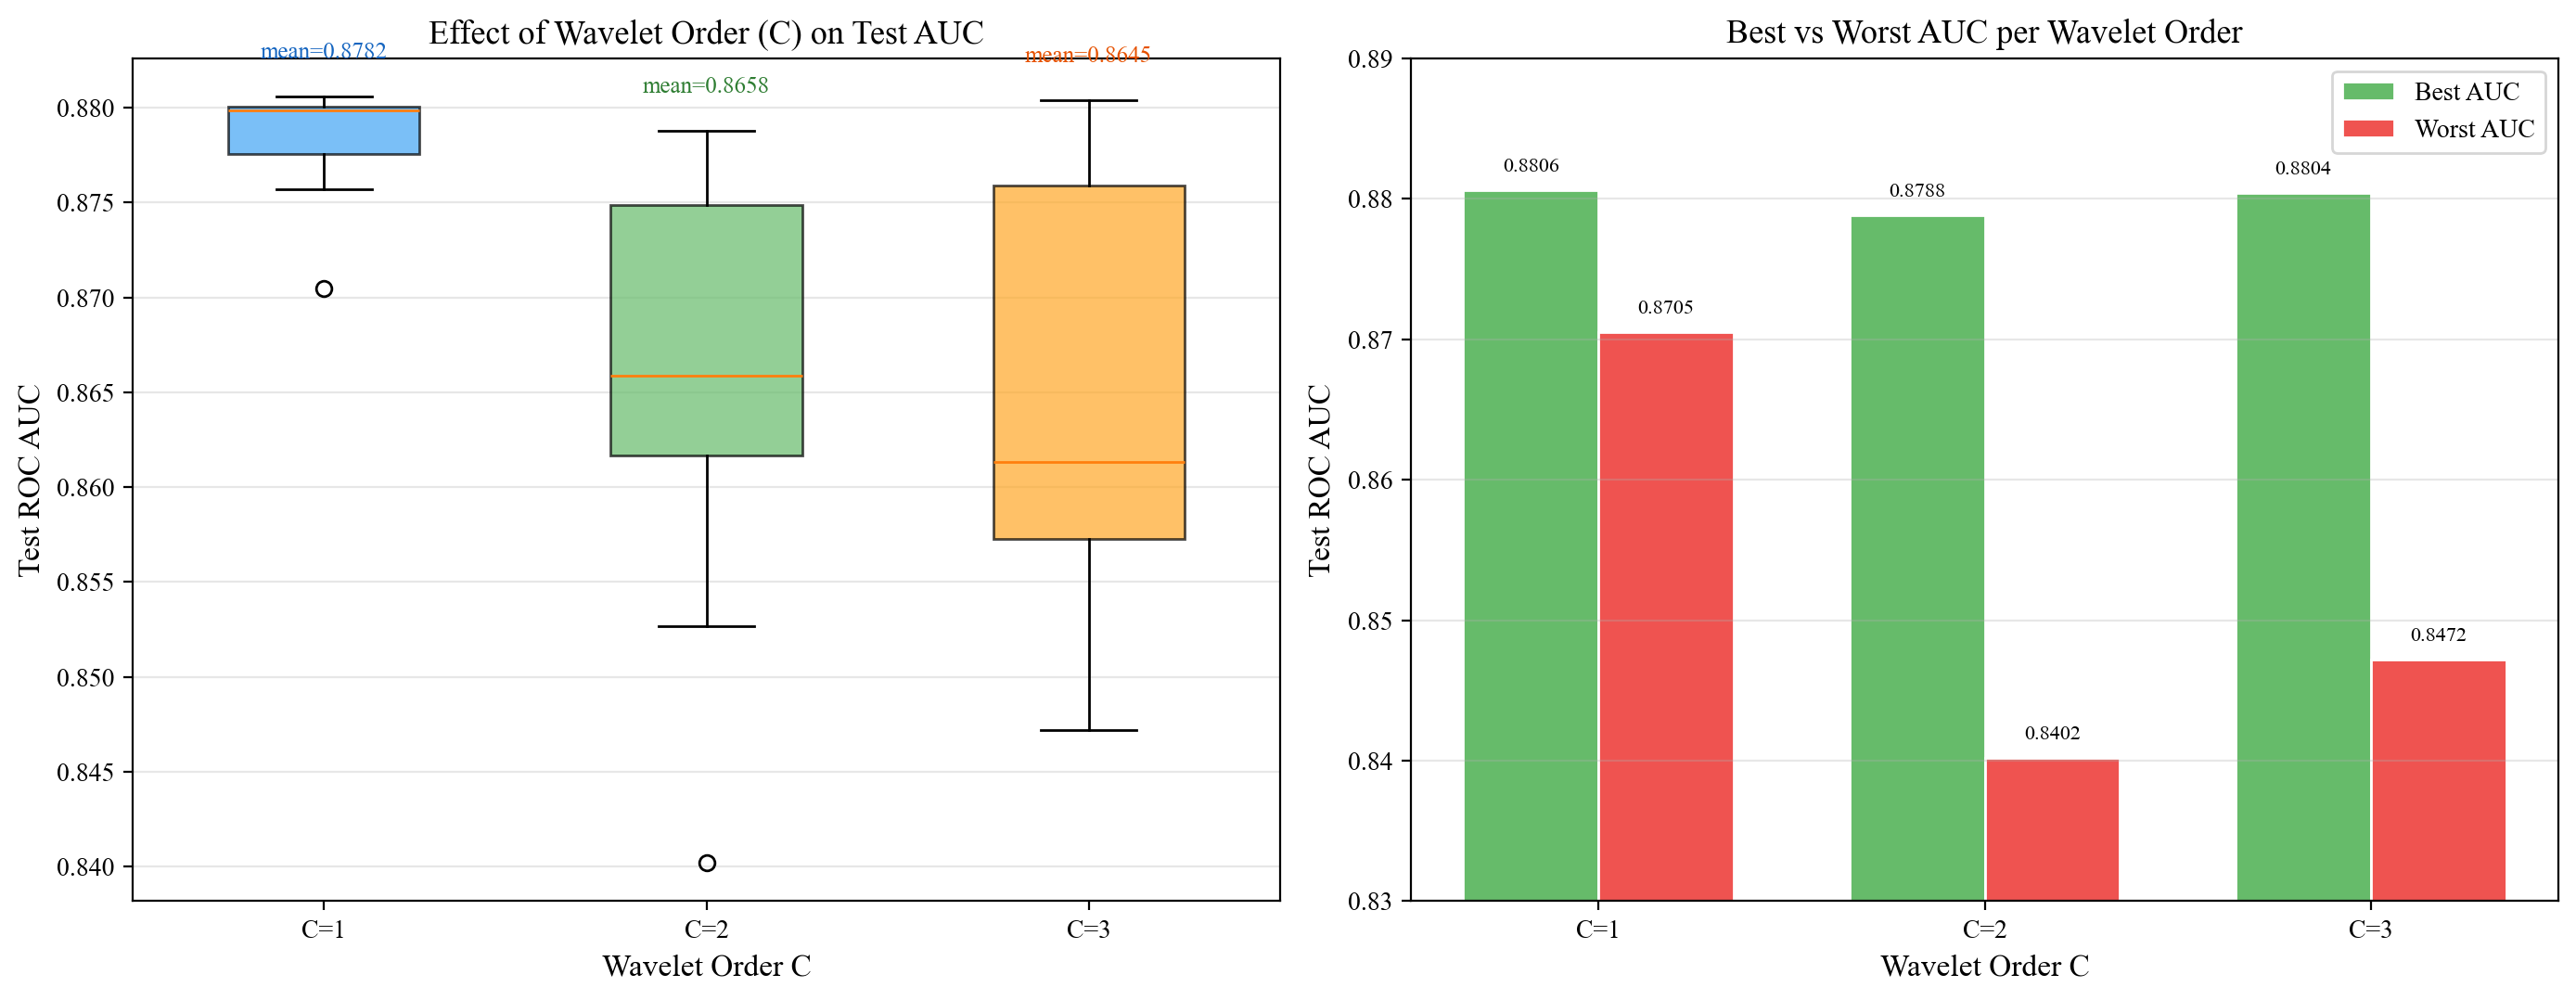
\includegraphics[width=0.85\textwidth]{figure_4}
\caption{Experiment 1 (Hidden Dim 128) --- ROC Curve and Confusion Matrix. The model achieved the best ROC AUC of 0.8859 with a TPR of 52.54\% at 5\% FPR.}
\label{fig:gnn-fig4}
\end{figure}

\begin{figure}[H]
\centering
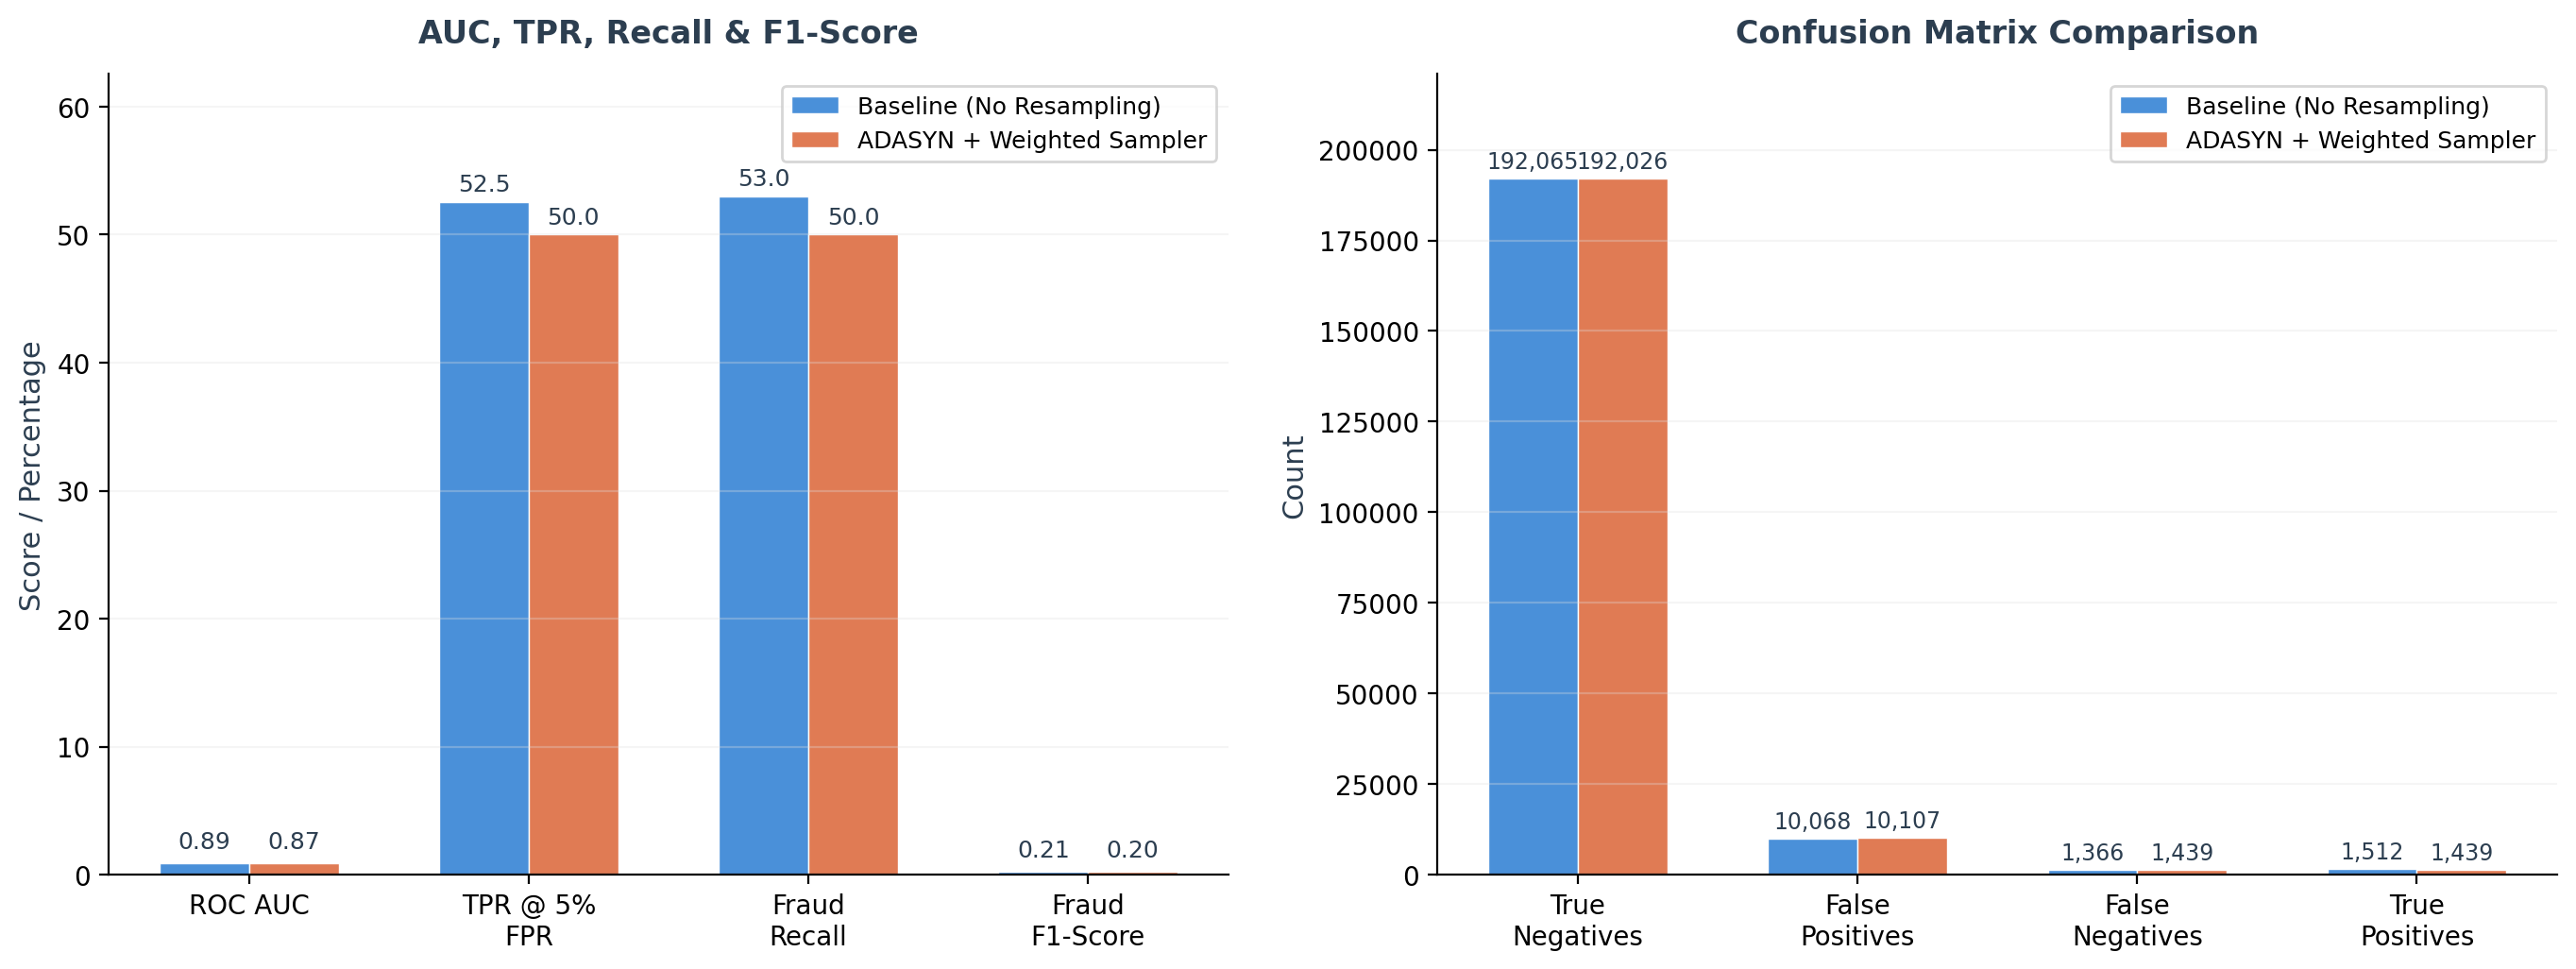
\includegraphics[width=0.85\textwidth]{figure_5}
\caption{Experiment 2 (Hidden Dim 64) --- ROC Curve and Confusion Matrix. The model achieved an AUC of 0.8829 with a TPR of 51.18\% at 5\% FPR.}
\label{fig:gnn-fig5}
\end{figure}

\subsubsection{QGNN Qubit and Depth Ablation}

\begin{figure}[H]
\centering
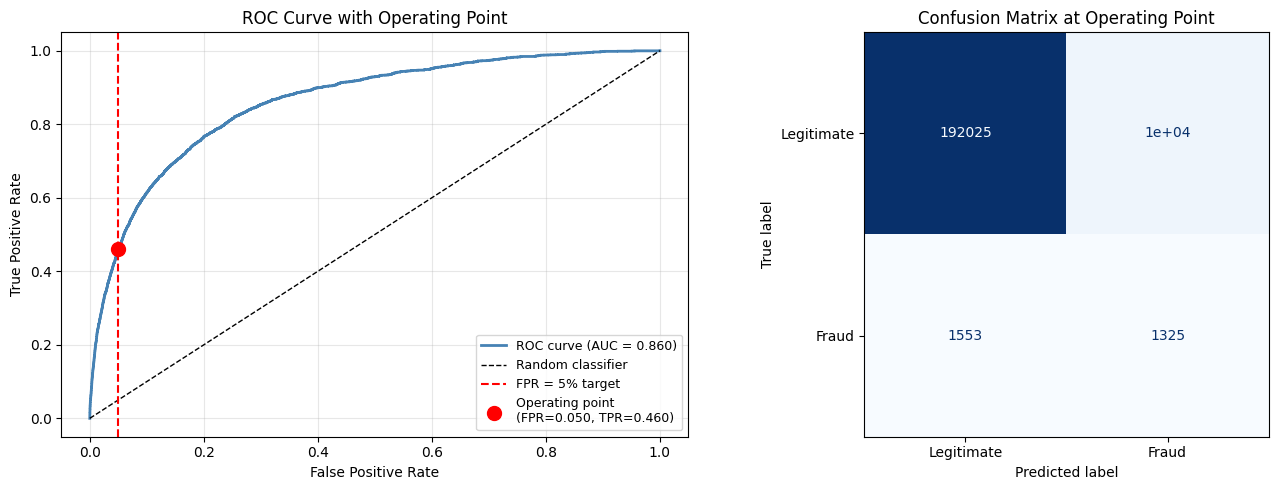
\includegraphics[width=0.85\textwidth]{figure_7}
\caption{Performance Comparison of QGNN Configurations. Dual-axis chart showing ROC AUC (blue, left) and TPR at 5\% FPR (orange, right).}
\label{fig:gnn-fig7}
\end{figure}

\begin{table}[H]
\centering
\caption{Confusion Matrix Details for All QGNN Experiments}
\label{tab:gnn-qgnn-confusion}
\small
\begin{tabularx}{0.9\textwidth}{lXrrrr}
\toprule
\textbf{Experiment} & \textbf{Threshold} & \textbf{TN} & \textbf{FP} & \textbf{FN} & \textbf{TP} \\
\midrule
1 (16Q, 4L) & 0.7983 & 192,032 & 10,101 & 1,461 & 1,417 \\
2 (6Q, 1L) & 0.7857 & 192,025 & 10,108 & 1,553 & 1,325 \\
3 (6Q, 2L) & 0.8223 & 192,018 & 10,115 & 1,588 & 1,290 \\
4 (16Q, 1L) & 0.7905 & 192,026 & 10,107 & 1,464 & 1,414 \\
\bottomrule
\end{tabularx}
\end{table}

\begin{figure}[H]
\centering
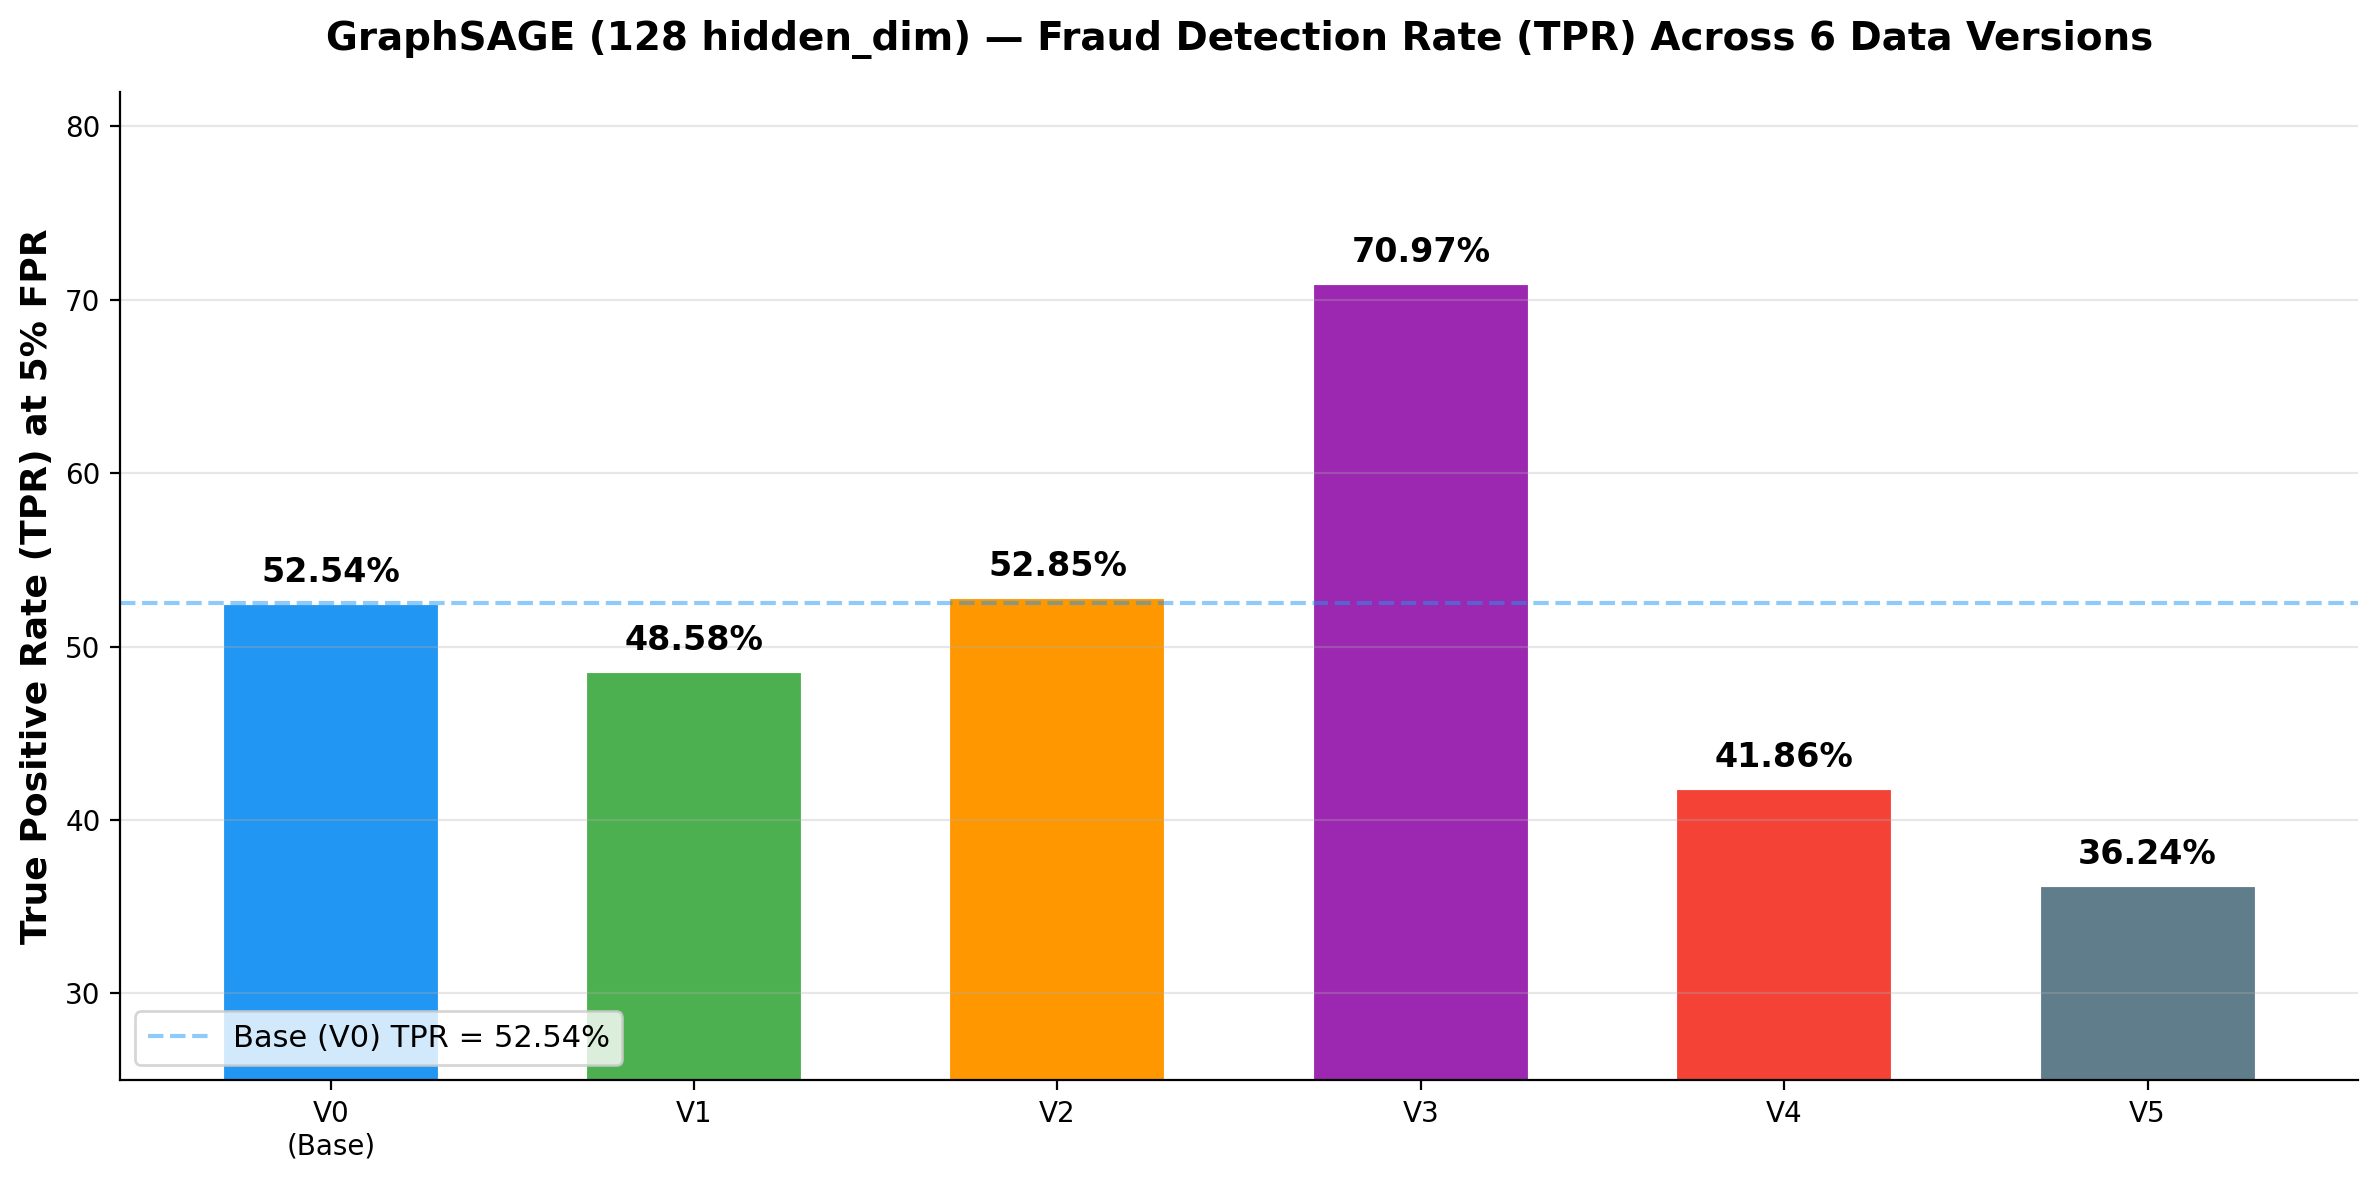
\includegraphics[width=0.85\textwidth]{figure_8}
\caption{Experiment 1 (16 Qubits, 4 Layers) --- ROC Curve and Confusion Matrix. Best QGNN configuration with AUC = 0.8769.}
\label{fig:gnn-fig8}
\end{figure}

\begin{figure}[H]
\centering
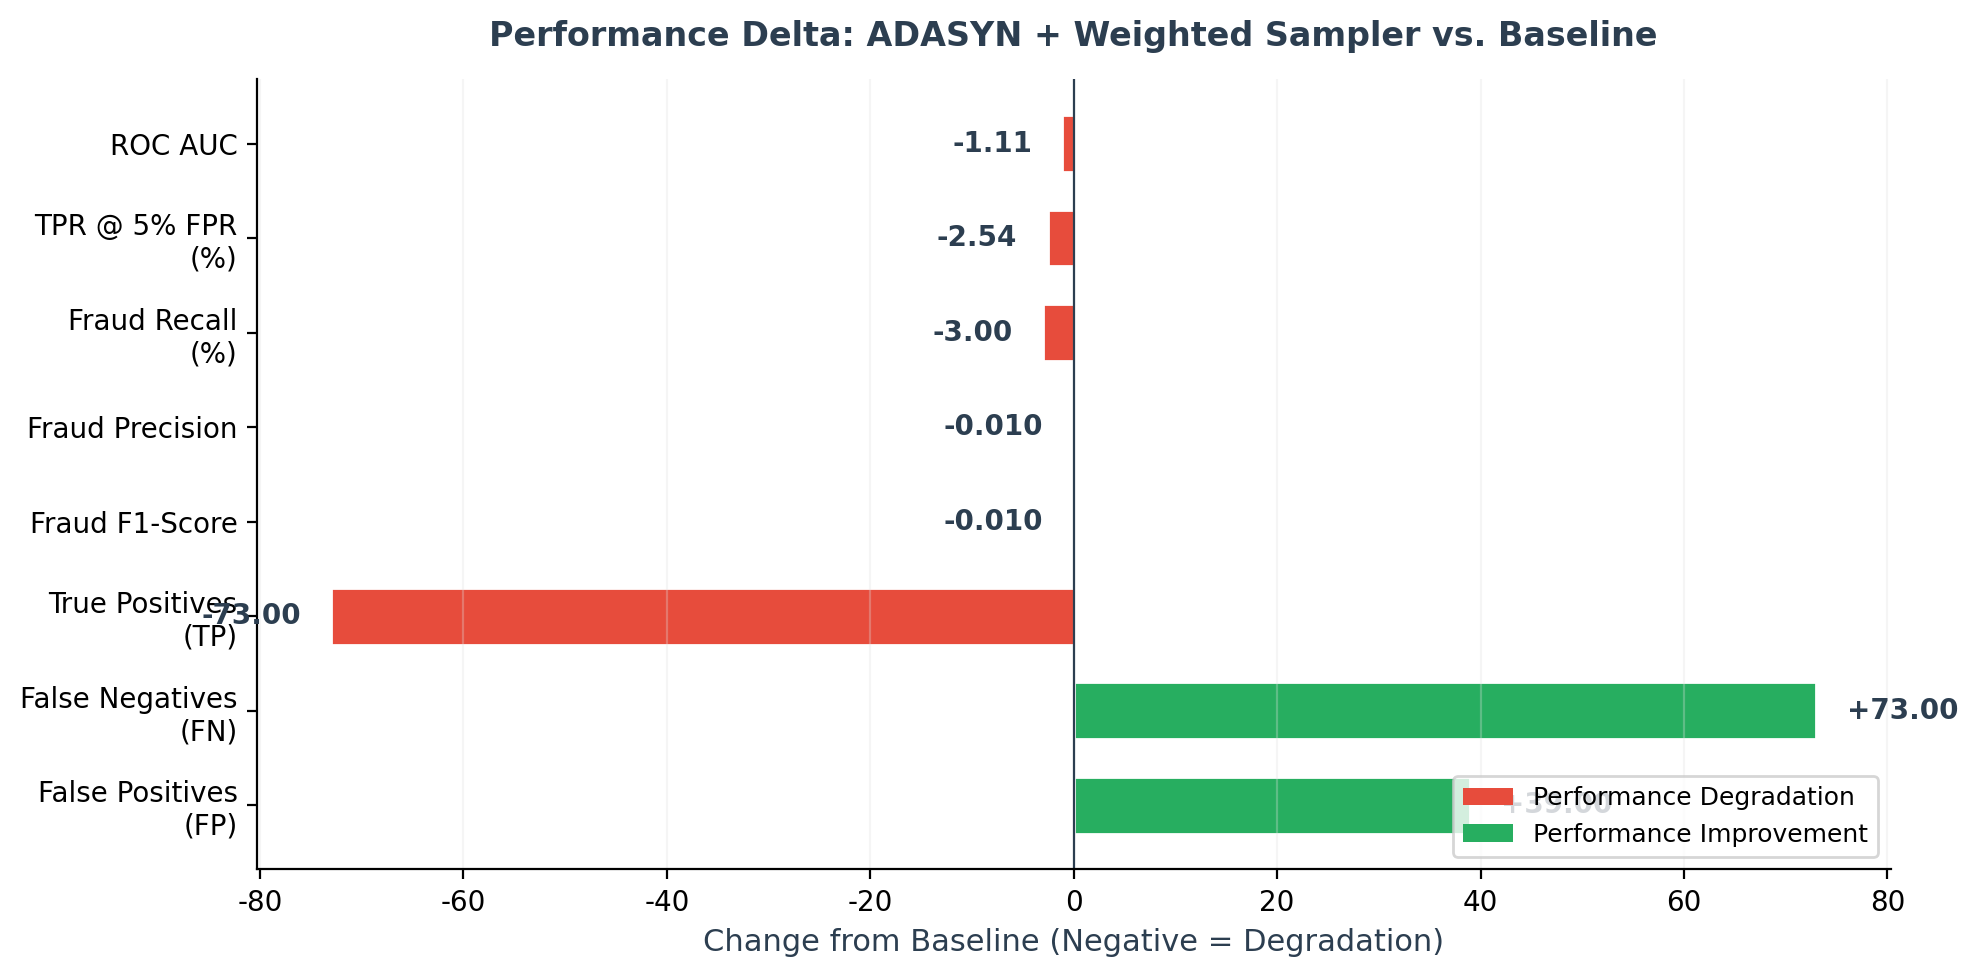
\includegraphics[width=0.85\textwidth]{figure_9}
\caption{Experiment 4 (16 Qubits, 1 Layer) --- ROC Curve and Confusion Matrix. AUC = 0.8731.}
\label{fig:gnn-fig9}
\end{figure}

\begin{figure}[H]
\centering
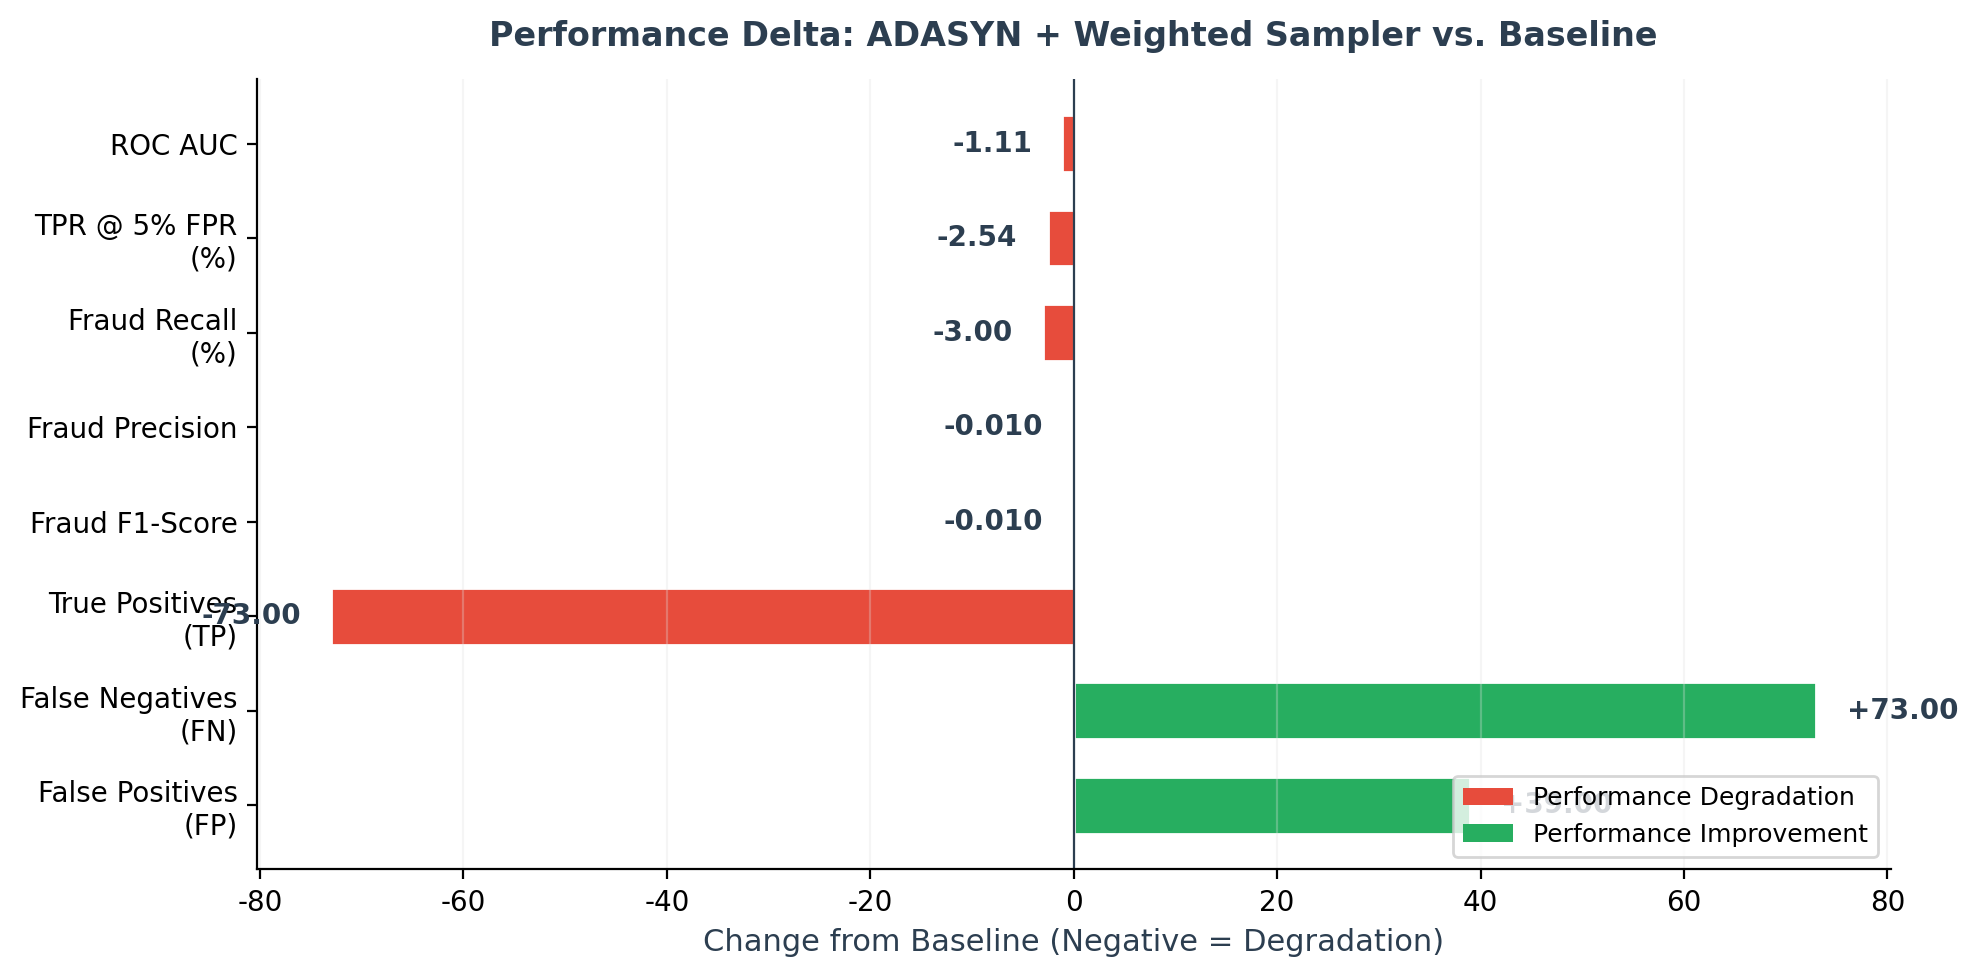
\includegraphics[width=0.85\textwidth]{figure_9}
\caption{Experiment 2 (6 Qubits, 1 Layer) --- ROC Curve and Confusion Matrix. AUC = 0.8602.}
\label{fig:gnn-fig10}
\end{figure}

\begin{figure}[H]
\centering
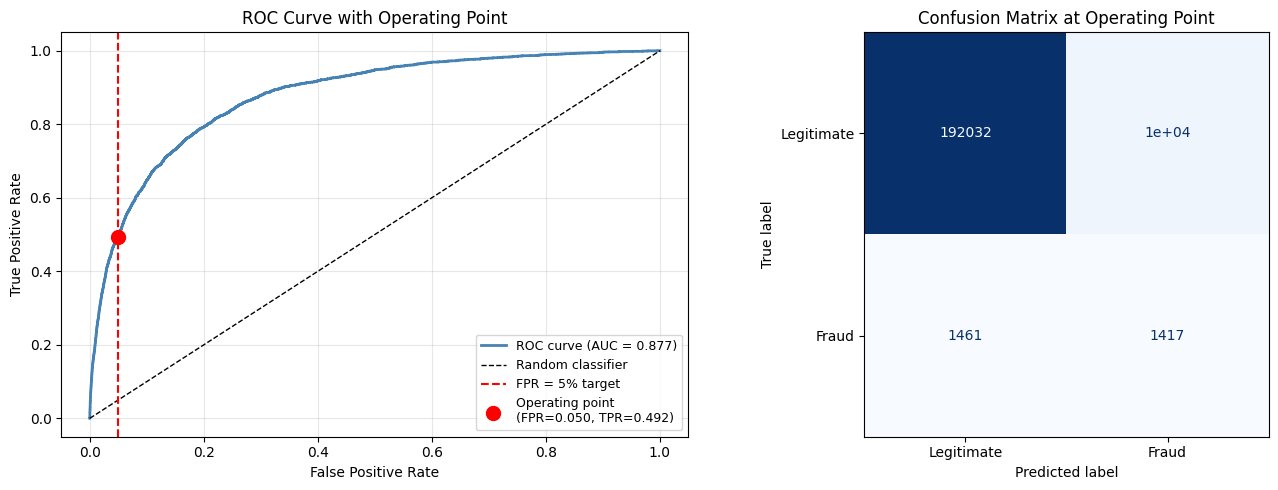
\includegraphics[width=0.85\textwidth]{figure_10}
\caption{Experiment 3 (6 Qubits, 2 Layers) --- ROC Curve and Confusion Matrix. AUC = 0.8574.}
\label{fig:gnn-qgnn-exp3-roc}
\end{figure}

\subsubsection{Split GNN Hyperparameter Ablation}

\paragraph{Effect of $\gamma_{\text{edge}}$ (Edge Loss Weight)}

\begin{figure}[H]
\centering
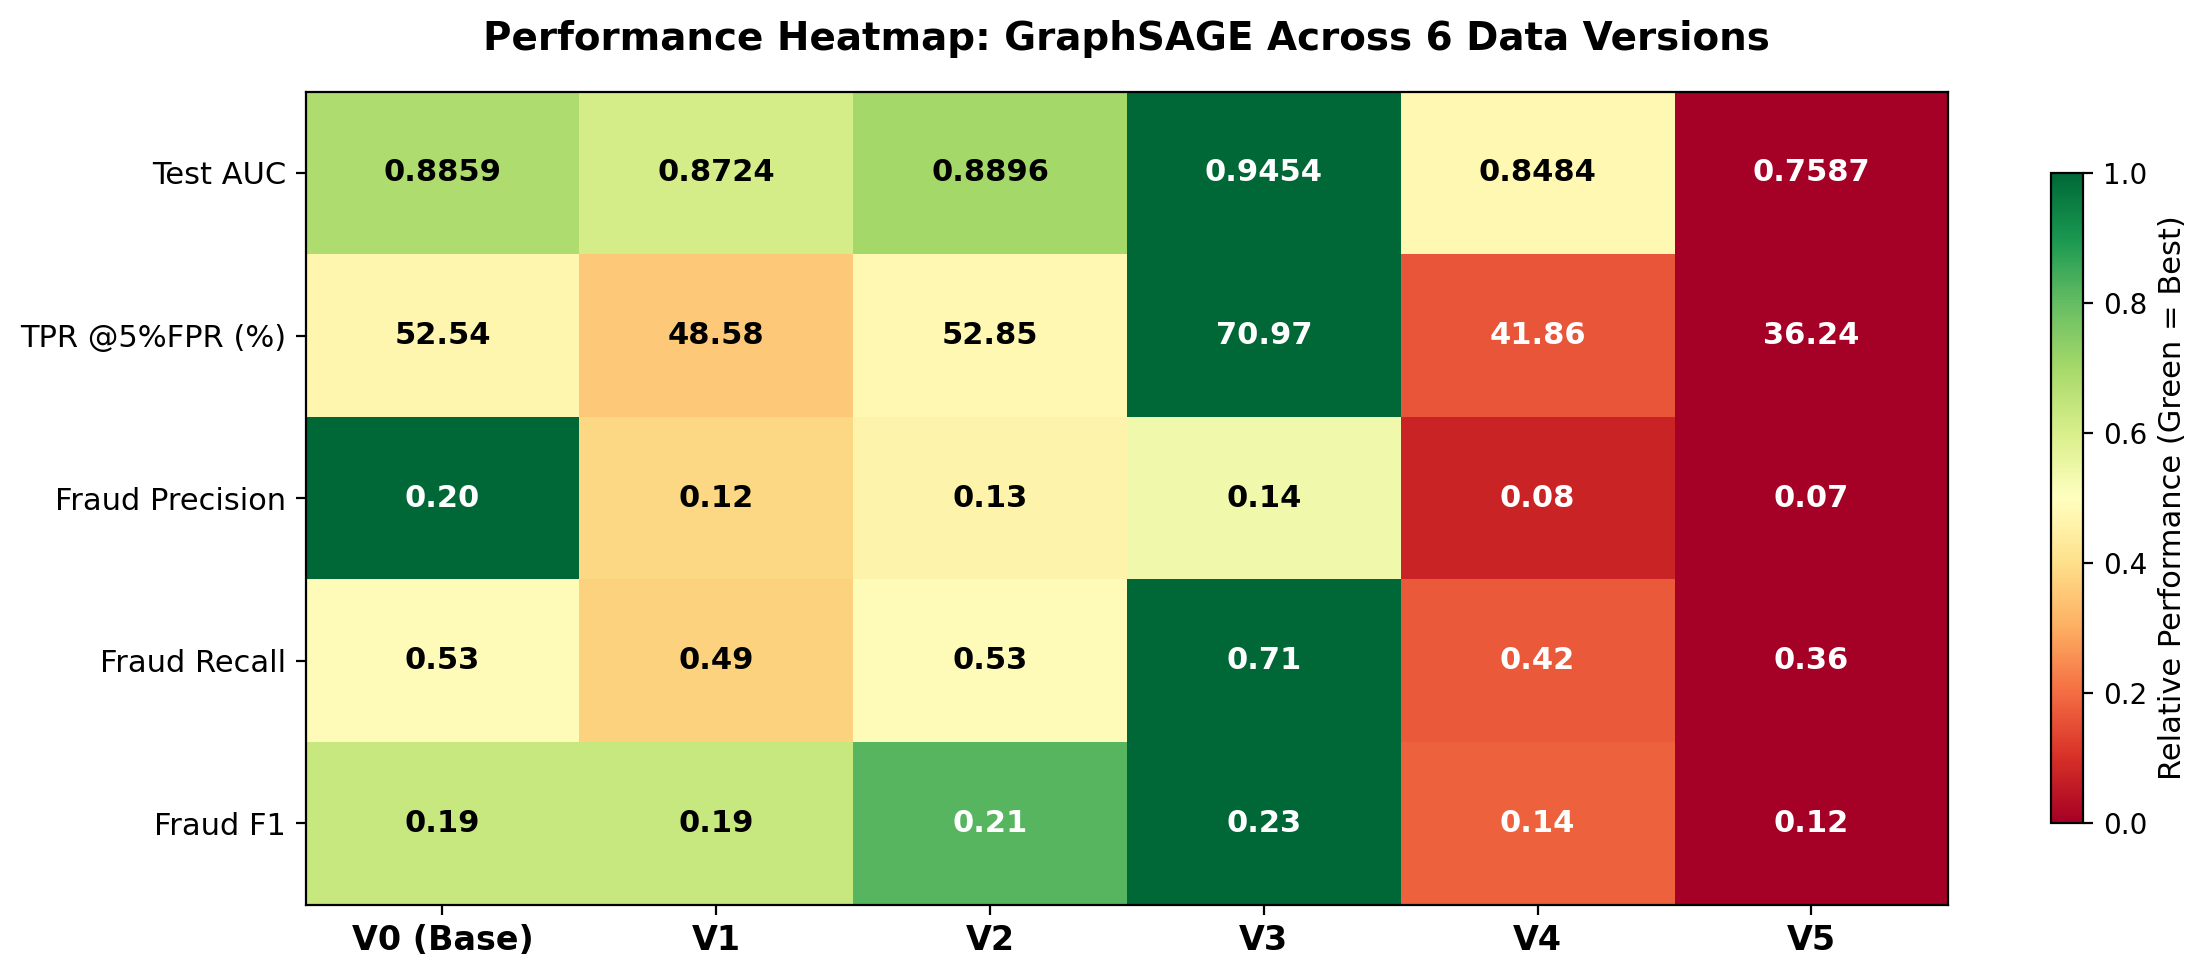
\includegraphics[width=0.85\textwidth]{figure_12}
\caption{Effect of $\gamma_{\text{edge}}$ on model performance --- best/mean/worst AUC (left) and fraud detection rate (right).}
\label{fig:gnn-fig12}
\end{figure}

\paragraph{Effect of Wavelet Order $C$}

\begin{figure}[H]
\centering
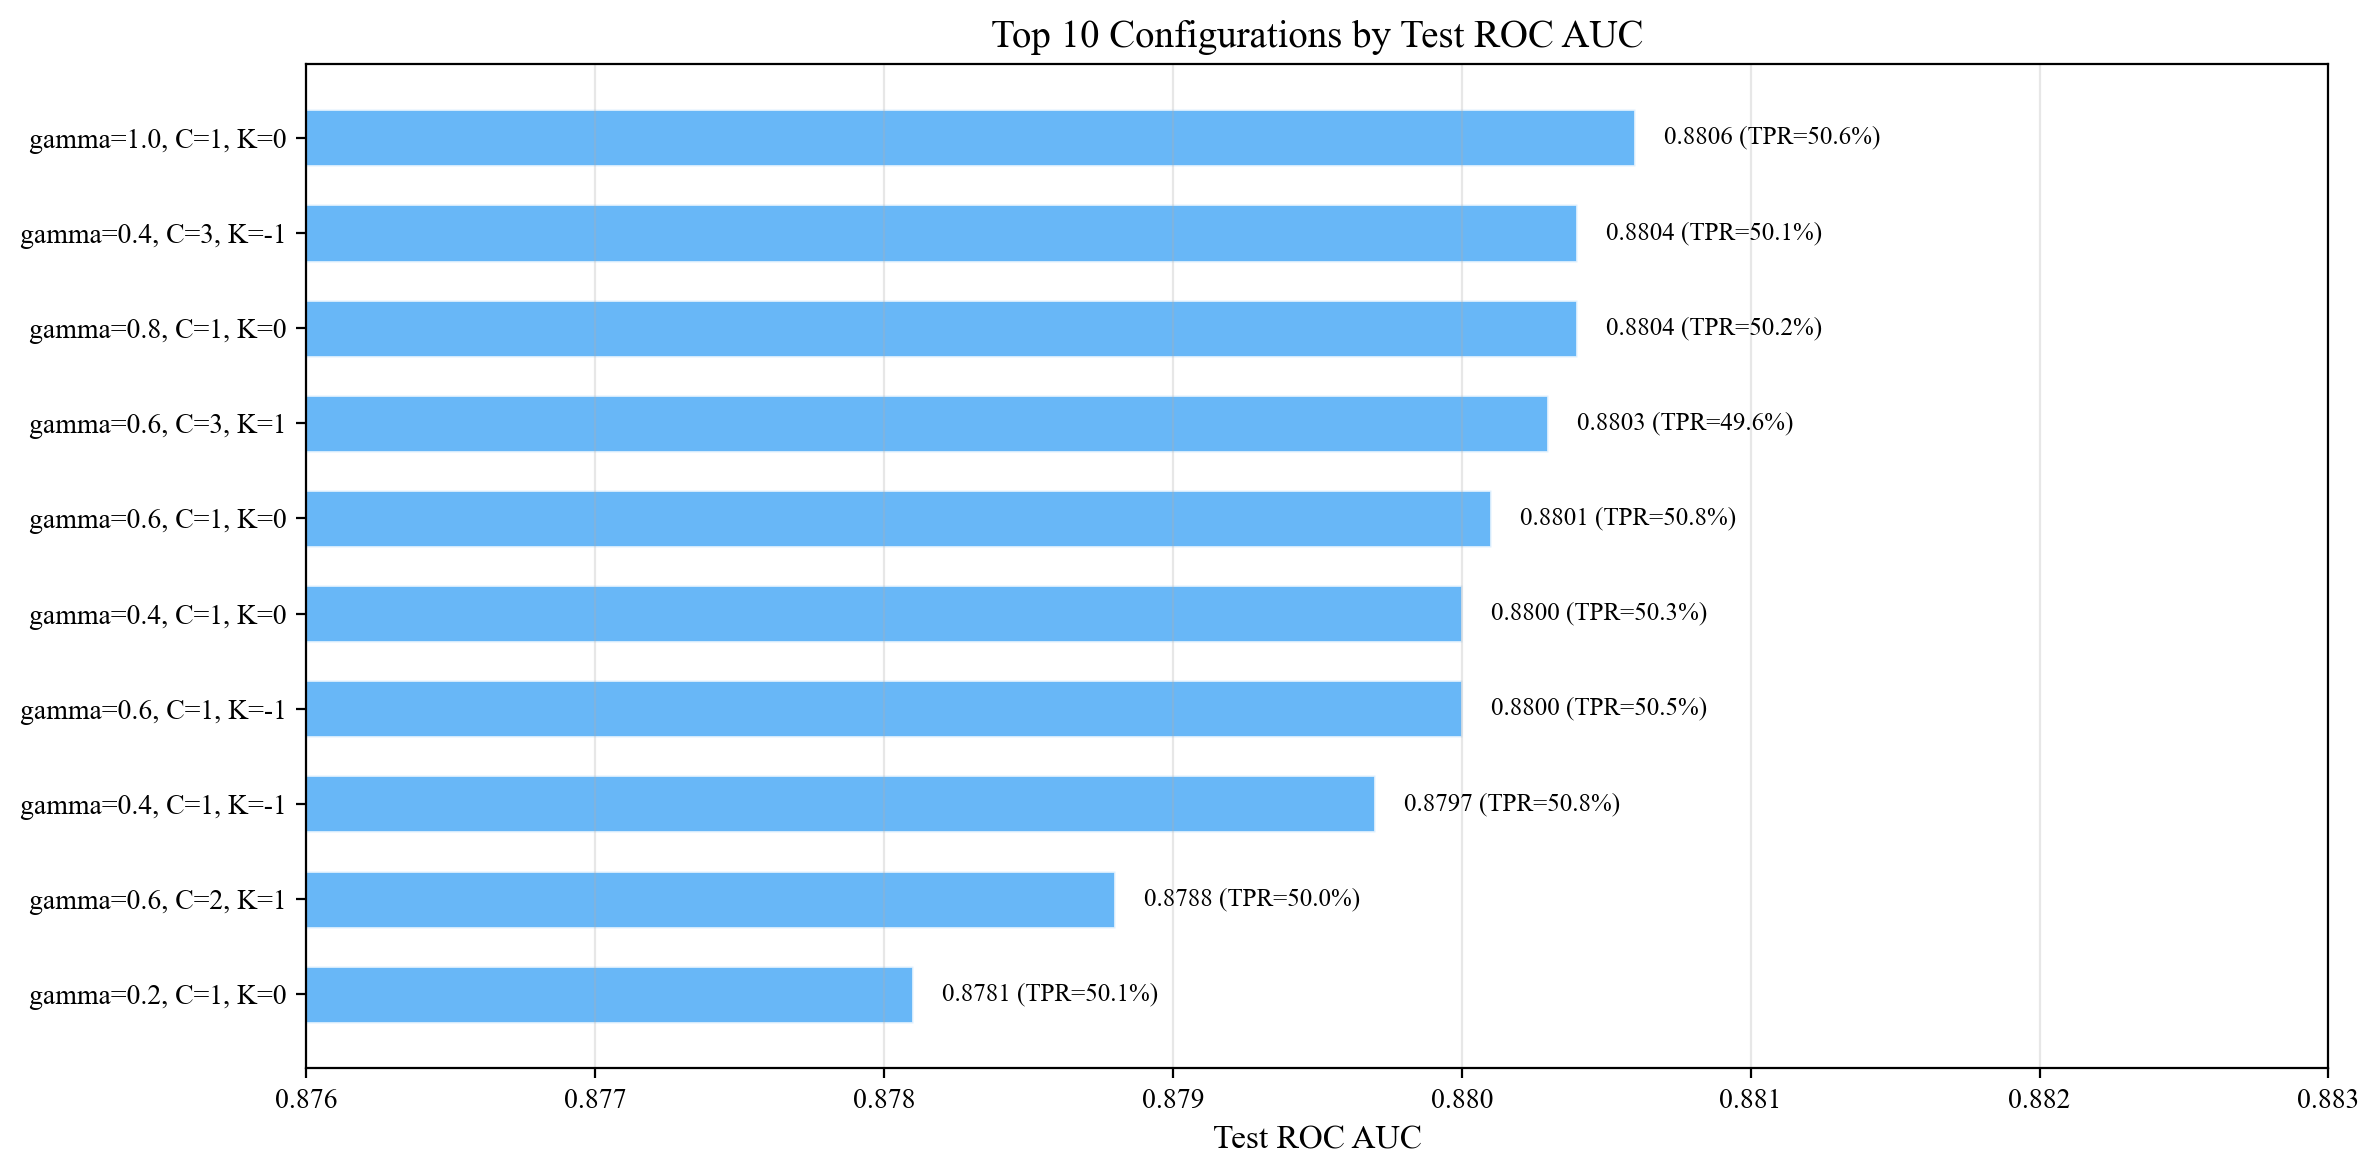
\includegraphics[width=0.85\textwidth]{figure_13}
\caption{Effect of wavelet order $C$ on Test AUC --- distribution box plots (left) and best vs worst comparison (right).}
\label{fig:gnn-fig13}
\end{figure}

\begin{table}[H]
\centering
\caption{Performance Summary by Wavelet Order}
\label{tab:gnn-wavelet-summary}
\small
\setlength{\tabcolsep}{4pt}
\begin{tabularx}{\textwidth}{Xrrrrr}
\toprule
\textbf{Wavelet Order $C$} & \textbf{Mean AUC} & \textbf{Best AUC} & \textbf{Worst AUC} & \textbf{Std Dev} & \textbf{\# Configs} \\
\midrule
$C = 1$ (2 bands) & 0.8789 & 0.8806 & 0.8705 & 0.003 & 10 \\
$C = 2$ (3 bands) & 0.8660 & 0.8788 & 0.8402 & 0.009 & 15 \\
$C = 3$ (4 bands) & 0.8665 & 0.8804 & 0.8472 & 0.010 & 20 \\
\bottomrule
\end{tabularx}
\end{table}

\paragraph{Effect of Split Point $K$}

\begin{figure}[H]
\centering
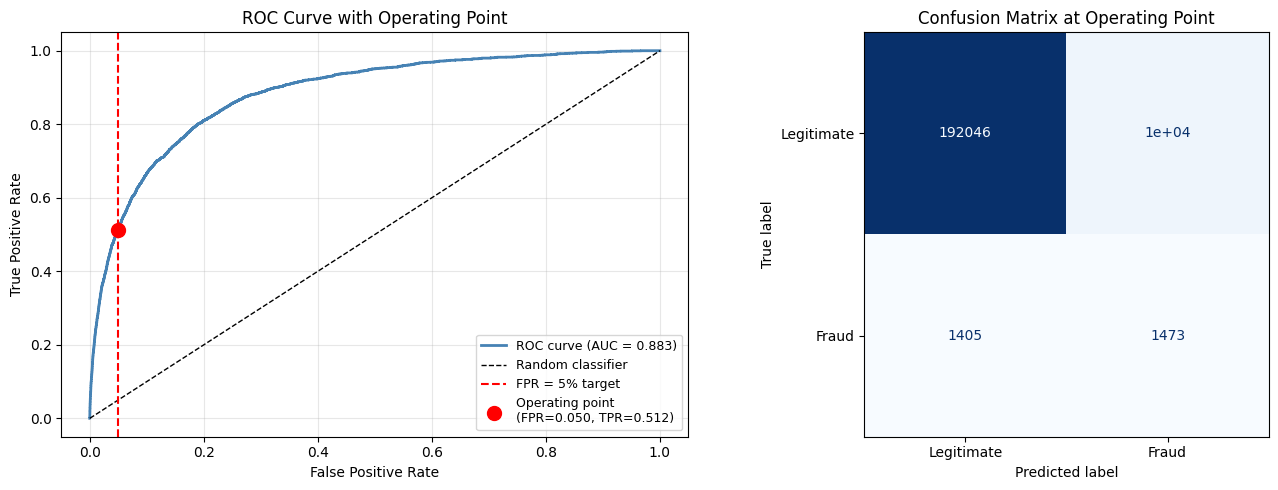
\includegraphics[width=0.85\textwidth]{figure_1}
\caption{Effect of split point $K$ on Test AUC --- distribution box plots (left) and interaction with wavelet order $C$ (right).}
\label{fig:gnn-k-effect}
\end{figure}

\paragraph{Complete 45-Experiment Results}

\begin{figure}[H]
\centering
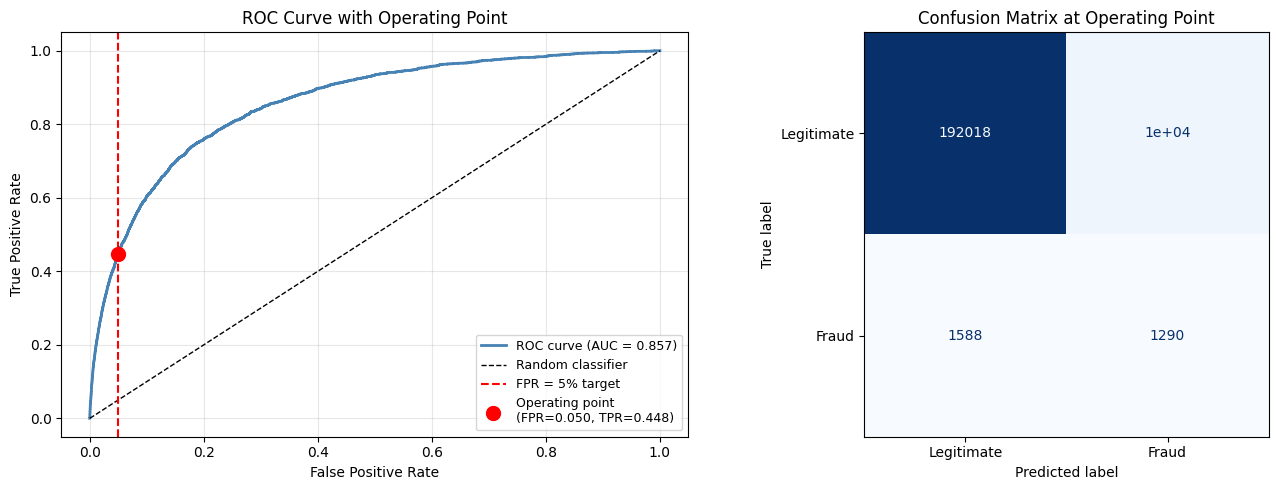
\includegraphics[width=0.85\textwidth]{figure_2}
\caption{Complete heatmap of Test ROC AUC across all 45 experiments, organized by $(C, K)$ configuration and $\gamma_{\text{edge}}$ value.}
\label{fig:gnn-ablation-heatmap}
\end{figure}

\begin{table}[H]
\centering
\caption{Top 10 Split GNN Configurations}
\label{tab:gnn-top10}
\small
\setlength{\tabcolsep}{5pt}
\begin{tabularx}{\textwidth}{cXrrr}
\toprule
\textbf{Rank} & \textbf{Configuration} & \textbf{Test AUC} & \textbf{TPR @ 5\% FPR} & \textbf{Val AUC} \\
\midrule
1 & $\gamma$=1.0, C=1, K=0 & 0.8806 & 50.6\% & 0.8808 \\
2 & $\gamma$=0.4, C=3, K=$-$1 & 0.8804 & 50.1\% & 0.8800 \\
3 & $\gamma$=0.8, C=1, K=0 & 0.8804 & 50.2\% & 0.8798 \\
4 & $\gamma$=0.6, C=3, K=1 & 0.8803 & 49.6\% & 0.8802 \\
5 & $\gamma$=0.6, C=1, K=0 & 0.8801 & 50.8\% & 0.8811 \\
6 & $\gamma$=0.4, C=1, K=0 & 0.8800 & 50.3\% & 0.8797 \\
7 & $\gamma$=0.6, C=1, K=$-$1 & 0.8800 & 50.5\% & 0.8792 \\
8 & $\gamma$=0.4, C=1, K=$-$1 & 0.8797 & 50.8\% & 0.8807 \\
9 & $\gamma$=0.6, C=2, K=1 & 0.8788 & 50.0\% & 0.8793 \\
10 & $\gamma$=0.2, C=1, K=0 & 0.8781 & 50.1\% & 0.8791 \\
\bottomrule
\end{tabularx}
\end{table}

\begin{figure}[H]
\centering
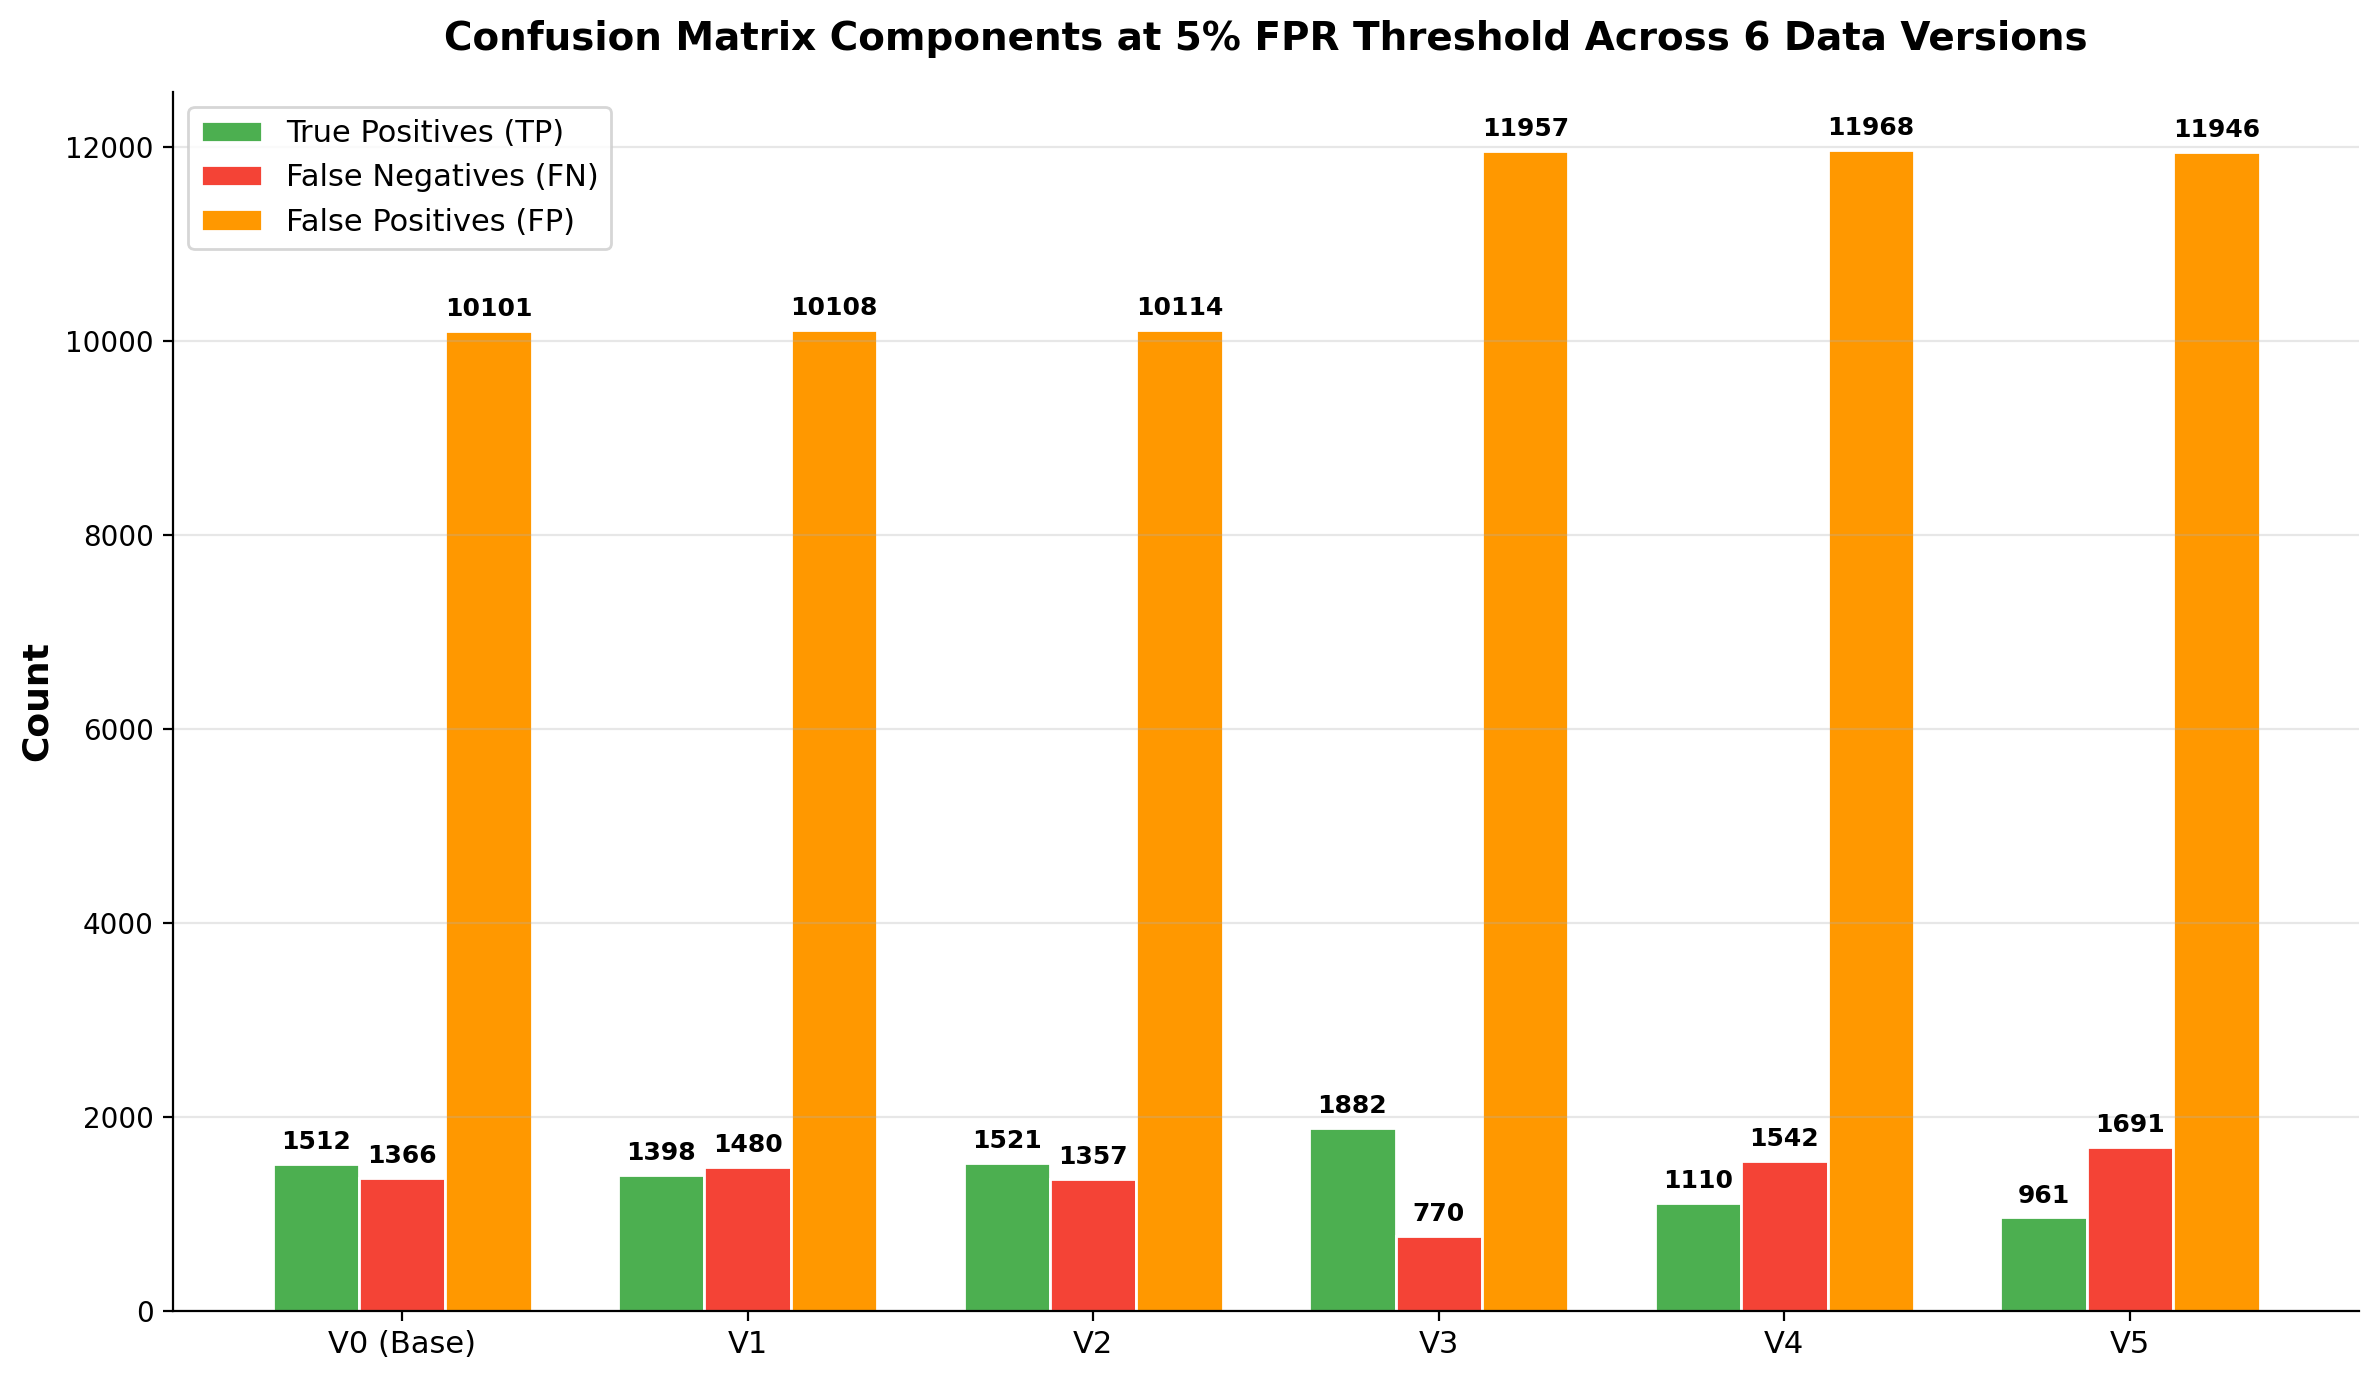
\includegraphics[width=0.85\textwidth]{figure_3}
\caption{Visual comparison of the top 10 configurations by Test ROC AUC and fraud detection rate.}
\label{fig:gnn-top10-visual}
\end{figure}

\begin{table}[H]
\centering
\caption{Bottom 5 Split GNN Configurations}
\label{tab:gnn-bottom5}
\small
\setlength{\tabcolsep}{5pt}
\begin{tabular}{cp{4.5cm}rrrr}
\toprule
\textbf{Rank} & \textbf{Configuration} & \textbf{Test AUC} & \textbf{TPR @ 5\% FPR} & \textbf{Fraud Prec.} & \textbf{Fraud Recall} \\
\midrule
41 & $\gamma$=1.0, C=2, K=$-$1 & 0.8402 & 31.5\% & 0.08 & 0.32 \\
42 & $\gamma$=0.2, C=3, K=$-$1 & 0.8480 & 34.9\% & 0.09 & 0.35 \\
43 & $\gamma$=0.6, C=3, K=$-$1 & 0.8472 & 38.6\% & 0.10 & 0.39 \\
44 & $\gamma$=0.8, C=2, K=$-$1 & 0.8527 & 41.4\% & 0.11 & 0.41 \\
45 & $\gamma$=0.2, C=3, K=2 & 0.8508 & 47.8\% & 0.12 & 0.48 \\
\bottomrule
\end{tabular}
\end{table}

\subsubsection{Cross-Version Fairness Ablation}

The cross-version fairness study evaluates the GraphSAGE architecture (hidden\_dim=128) across six data distribution variants (Version 0 through Version V).

\begin{landscape}
\begin{table}[H]
\centering
\caption{Experiment Configuration and Dataset Characteristics Across All Six Data Versions}
\label{tab:gnn-version-configs}
\small
\setlength{\tabcolsep}{5pt}
\begin{tabular}{lrrrrrrr}
\toprule
\textbf{Version} & \textbf{Edges} & \textbf{Train} & \textbf{Val} & \textbf{Test} & \textbf{Train Fraud} & \textbf{Train Legit} & \textbf{Fraud Wt.} \\
\midrule
V0 (Base) & 14,491,868 & 675,666 & 119,324 & 205,010 & 6,740 & 668,926 & 99.25 \\
V I & 14,479,509 & 675,668 & 119,322 & 205,010 & 6,740 & 668,928 & 99.25 \\
V II & 14,547,755 & 675,666 & 119,324 & 205,010 & 6,740 & 668,926 & 99.25 \\
V III & 14,541,726 & 610,832 & 147,496 & 241,672 & 7,036 & 603,796 & 85.82 \\
V IV & 14,541,548 & 610,832 & 147,496 & 241,672 & 7,036 & 603,796 & 85.82 \\
V V & 14,542,330 & 610,832 & 147,496 & 241,672 & 7,036 & 603,796 & 85.82 \\
\bottomrule
\end{tabular}
\end{table}
\end{landscape}

\subsubsection{Resampling Strategy Ablation}

\begin{table}[H]
\centering
\caption{Resampling Experiment Configuration Comparison}
\label{tab:gnn-resample-config}
\small
\begin{tabularx}{0.95\textwidth}{lXX}
\toprule
\textbf{Parameter} & \textbf{Baseline} & \textbf{Resampling Experiment} \\
\midrule
Architecture & GraphSAGE & GraphSAGE \\
Hidden Dimension & 128 & 128 \\
Data Version & V0 (Base) & V0 (Base) \\
Train / Val / Test Split & 675,666 / 119,323 / 205,011 & 675,666 / 119,323 / 205,011 \\
Split Strategy & Temporal & Temporal \\
Graph Nodes & 1,000,047 & 1,000,047 \\
Class Weight (Fraud) & 96.53 & 10.00 \\
Class Weight (Legitimate) & 1.00 & 0.05 \\
Weight Strategy & Inverse Frequency & ADASYN-Informed \\
Training Sampler & Standard & WeightedRandomSampler \\
\bottomrule
\end{tabularx}
\end{table}

\subsection{Statistical Significance Testing}

The performance differences between architectures were evaluated using bootstrap resampling with 1,000 iterations to estimate 95\% confidence intervals for the ROC AUC metric. Additionally, the Split GNN hyperparameter study provides distributional statistics (mean, standard deviation, best, worst) across the 45-experiment grid, enabling assessment of whether observed performance differences are statistically meaningful given the configuration variance.

\section{Results and Discussion}

\subsection{GraphSAGE Results}

Experiment 1 (hidden dimension 128) yielded the best overall performance with a test ROC AUC of 0.8859 and a True Positive Rate of 52.54\% at the 5\% FPR operating threshold. The model trained for 188 epochs before early stopping triggered (best validation AUC of 0.8858). The model correctly identified 1,512 out of 2,878 fraud cases while maintaining a low false positive count of 10,068 out of 202,133 legitimate transactions.

Experiment 2 (hidden dimension 64) achieved a test ROC AUC of 0.8829 and a TPR of 51.18\% at the 5\% FPR threshold. While the performance drop relative to Experiment 1 is modest (0.0030 AUC, 1.36\% TPR), the smaller model trained for fewer epochs (158 vs.\ 188) and would offer faster inference in a production setting.

\subsection{QGNN Results}

The best QGNN configuration (16 qubits, 4 VQC layers) achieved a peak ROC AUC of 0.8769 and a TPR of 49.24\% at 5\% FPR. The 6-qubit experiments showed a notable decline in performance, with Experiment 3 (6Q, 2L) dropping to 0.8574. Adding a second VQC layer to the 6-qubit model degraded performance, indicating that compressing features into 6 qubits creates a representational bottleneck where additional depth leads to overfitting without improved generalization.

The comparative analysis reveals that the classical GraphSAGE model outperforms the best QGNN configuration across all key metrics. The GraphSAGE achieves a higher ROC AUC (0.8859 vs.\ 0.8769) and a significantly better TPR at the 5\% FPR operating point (52.54\% vs.\ 49.24\%).

\begin{table}[H]
\centering
\caption{GraphSAGE vs.\ QGNN Best Configuration Comparison}
\label{tab:gnn-sage-vs-qgnn}
\small
\begin{tabularx}{0.8\textwidth}{Xrrr}
\toprule
\textbf{Metric} & \textbf{GraphSAGE (Best)} & \textbf{QGNN (Best)} & \textbf{Difference} \\
\midrule
ROC AUC & 0.8859 & 0.8769 & $-$0.0090 \\
TPR @ 5\% FPR & 52.54\% & 49.24\% & $-$3.30\% \\
Fraud Recall & 53\% & 49\% & $-$4\% \\
True Positives & 1,512 & 1,417 & $-$95 \\
\bottomrule
\end{tabularx}
\end{table}

\subsection{Split GNN Results}

Based on the comprehensive analysis of 45 experiments, the recommended optimal configuration for the Split GNN architecture is $C = 1$, $K = 0$, with $\gamma_{\text{edge}}$ in the range $[0.4, 1.0]$. This configuration achieves the highest peak AUC of 0.8806 and the most robust average performance across $\gamma$ values. The simplicity of $C = 1$ (only 2 wavelet bands) is a significant practical advantage, reducing memory usage by approximately 60\% compared to $C = 3$ while simultaneously improving performance.

\begin{landscape}
\begin{table}[H]
\centering
\caption{Best Split GNN Configuration per $\gamma_{\text{edge}}$ --- Detailed Classification Report}
\label{tab:gnn-split-classification}
\small
\setlength{\tabcolsep}{8pt}
\begin{tabularx}{\linewidth}{cXrrrrrrrrr}
\toprule
$\gamma$ & Best $(C,K)$ & Test AUC & Thr. & Leg.\ P & Leg.\ R & Fr.\ P & Fr.\ R & Fr.\ F1 & TP & FN \\
\midrule
0.2 & C=1, K=0 & 0.8781 & 0.5331 & 0.99 & 0.95 & 0.12 & 0.50 & 0.19 & 1,442 & 1,436 \\
0.4 & C=3, K=$-$1 & 0.8804 & 0.5220 & 0.99 & 0.95 & 0.12 & 0.50 & 0.20 & 1,443 & 1,435 \\
0.6 & C=3, K=1 & 0.8803 & 0.5244 & 0.99 & 0.95 & 0.12 & 0.50 & 0.20 & 1,429 & 1,449 \\
0.8 & C=1, K=0 & 0.8804 & 0.5085 & 0.99 & 0.95 & 0.13 & 0.50 & 0.20 & 1,445 & 1,433 \\
1.0 & C=1, K=0 & 0.8806 & 0.5121 & 0.99 & 0.95 & 0.13 & 0.51 & 0.20 & 1,456 & 1,422 \\
\bottomrule
\end{tabularx}
\end{table}
\end{landscape}

\subsection{Cross-Version Fairness Results}

The cross-version evaluation reveals substantial variation in model performance across the six data versions.

\begin{figure}[H]
\centering
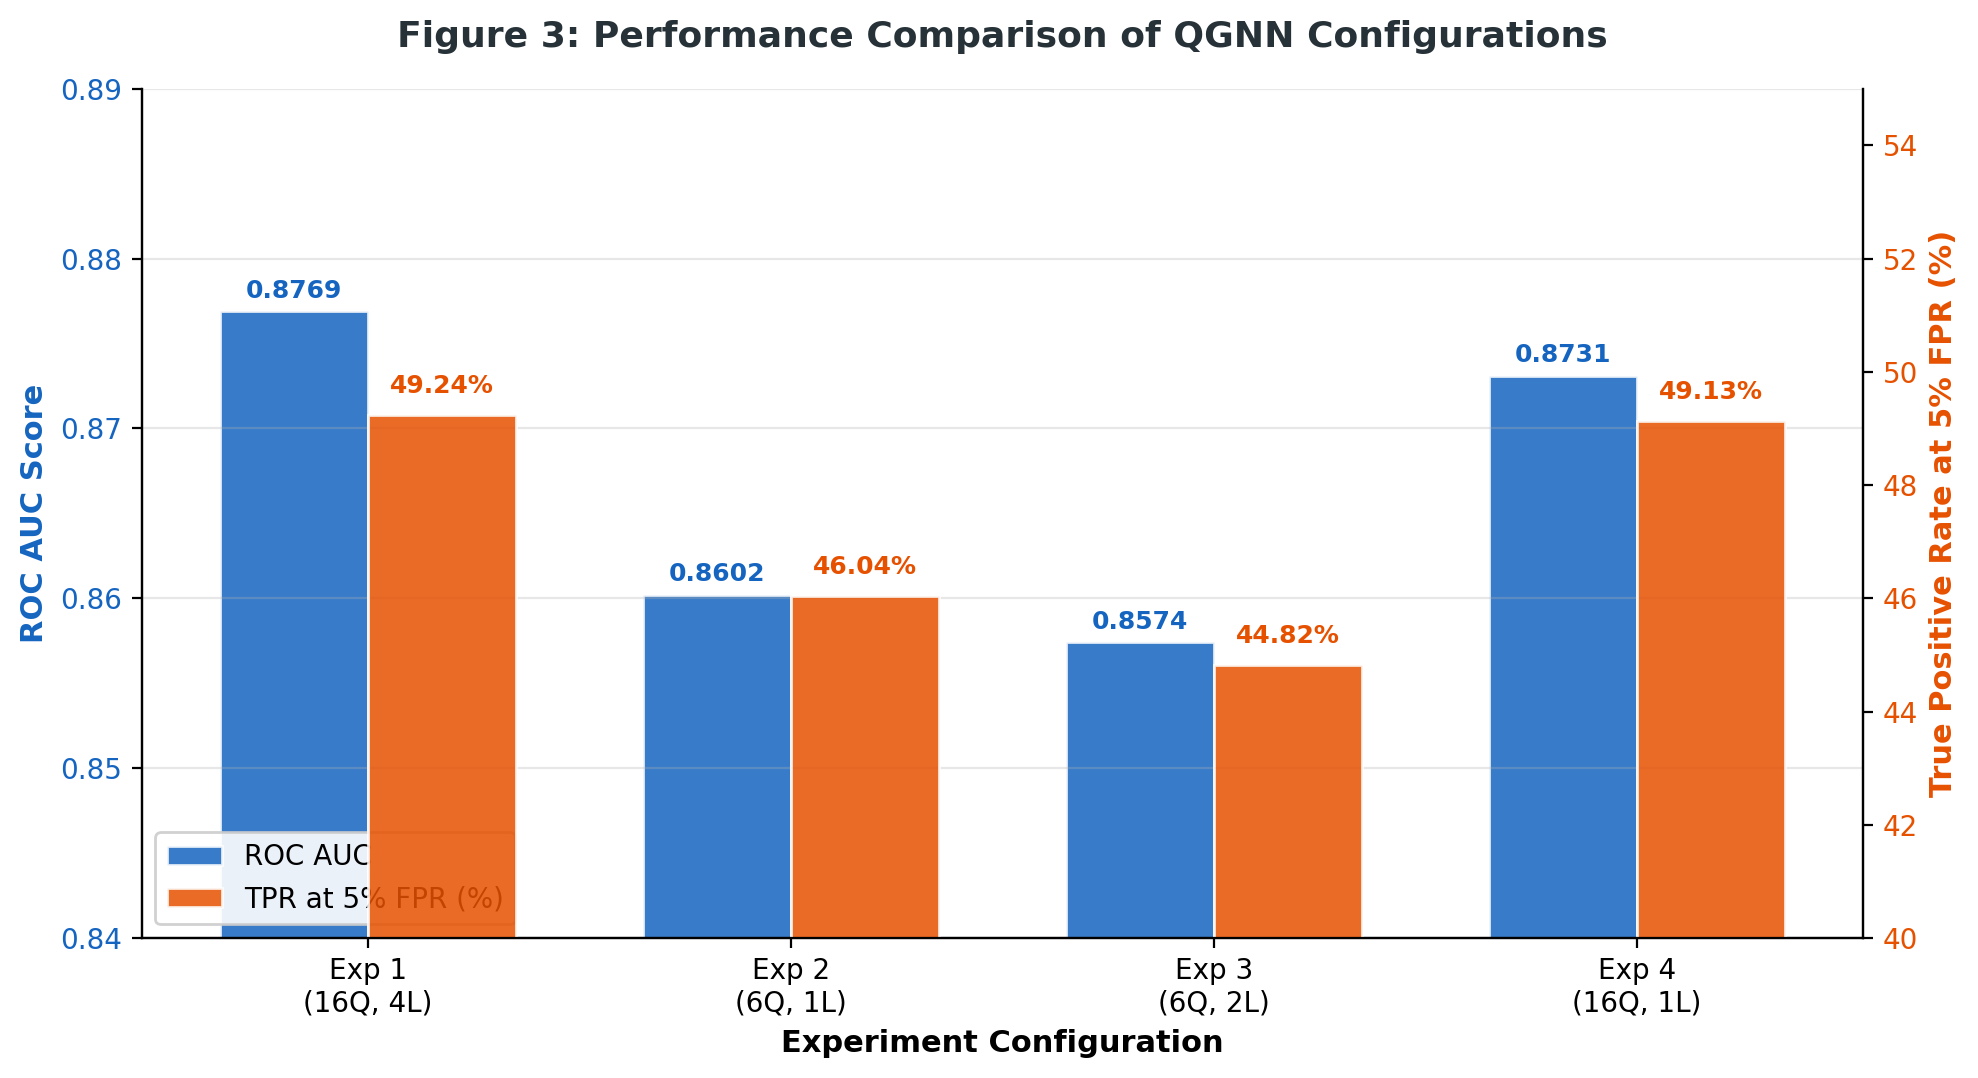
\includegraphics[width=0.85\textwidth]{figure_16}
\caption{Test ROC AUC comparison across all six data versions. The dashed blue line represents the base version benchmark (AUC = 0.8859).}
\label{fig:gnn-fig16}
\end{figure}

\begin{figure}[H]
\centering
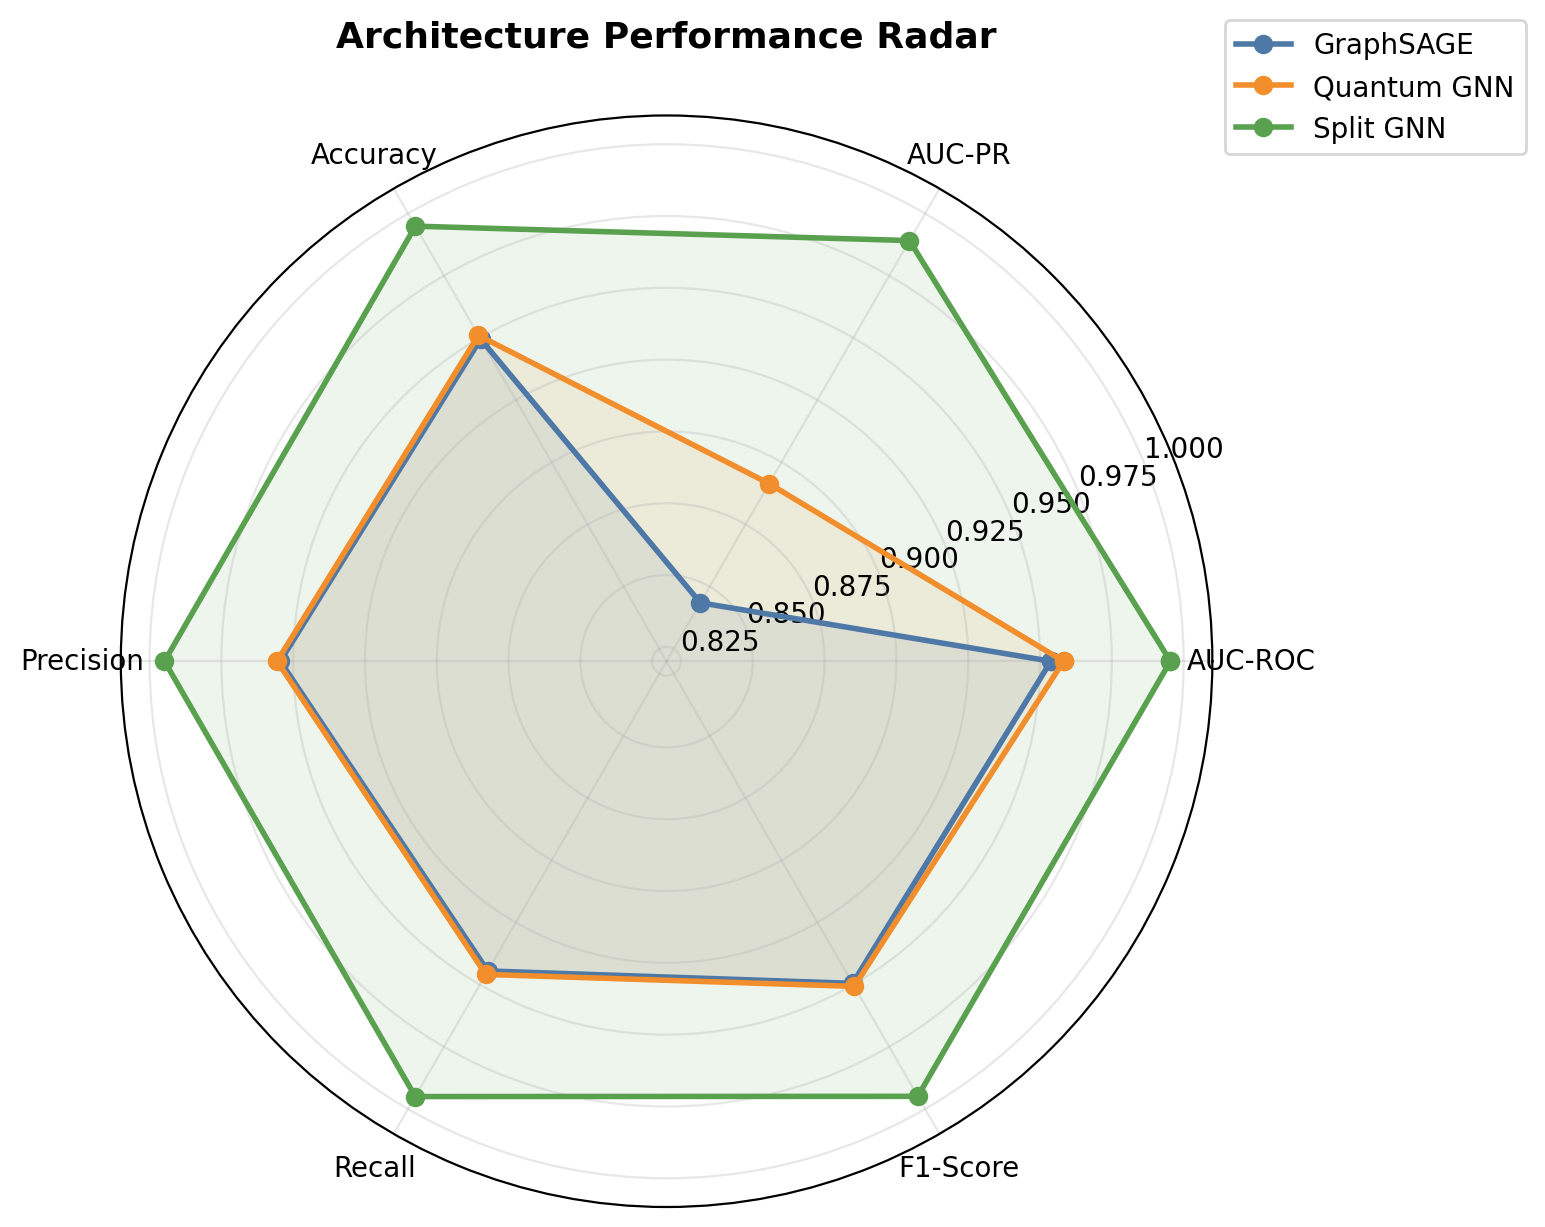
\includegraphics[width=0.85\textwidth]{figure_17}
\caption{True Positive Rate (TPR) at 5\% FPR threshold across all six data versions.}
\label{fig:gnn-fig17}
\end{figure}

\begin{figure}[H]
\centering
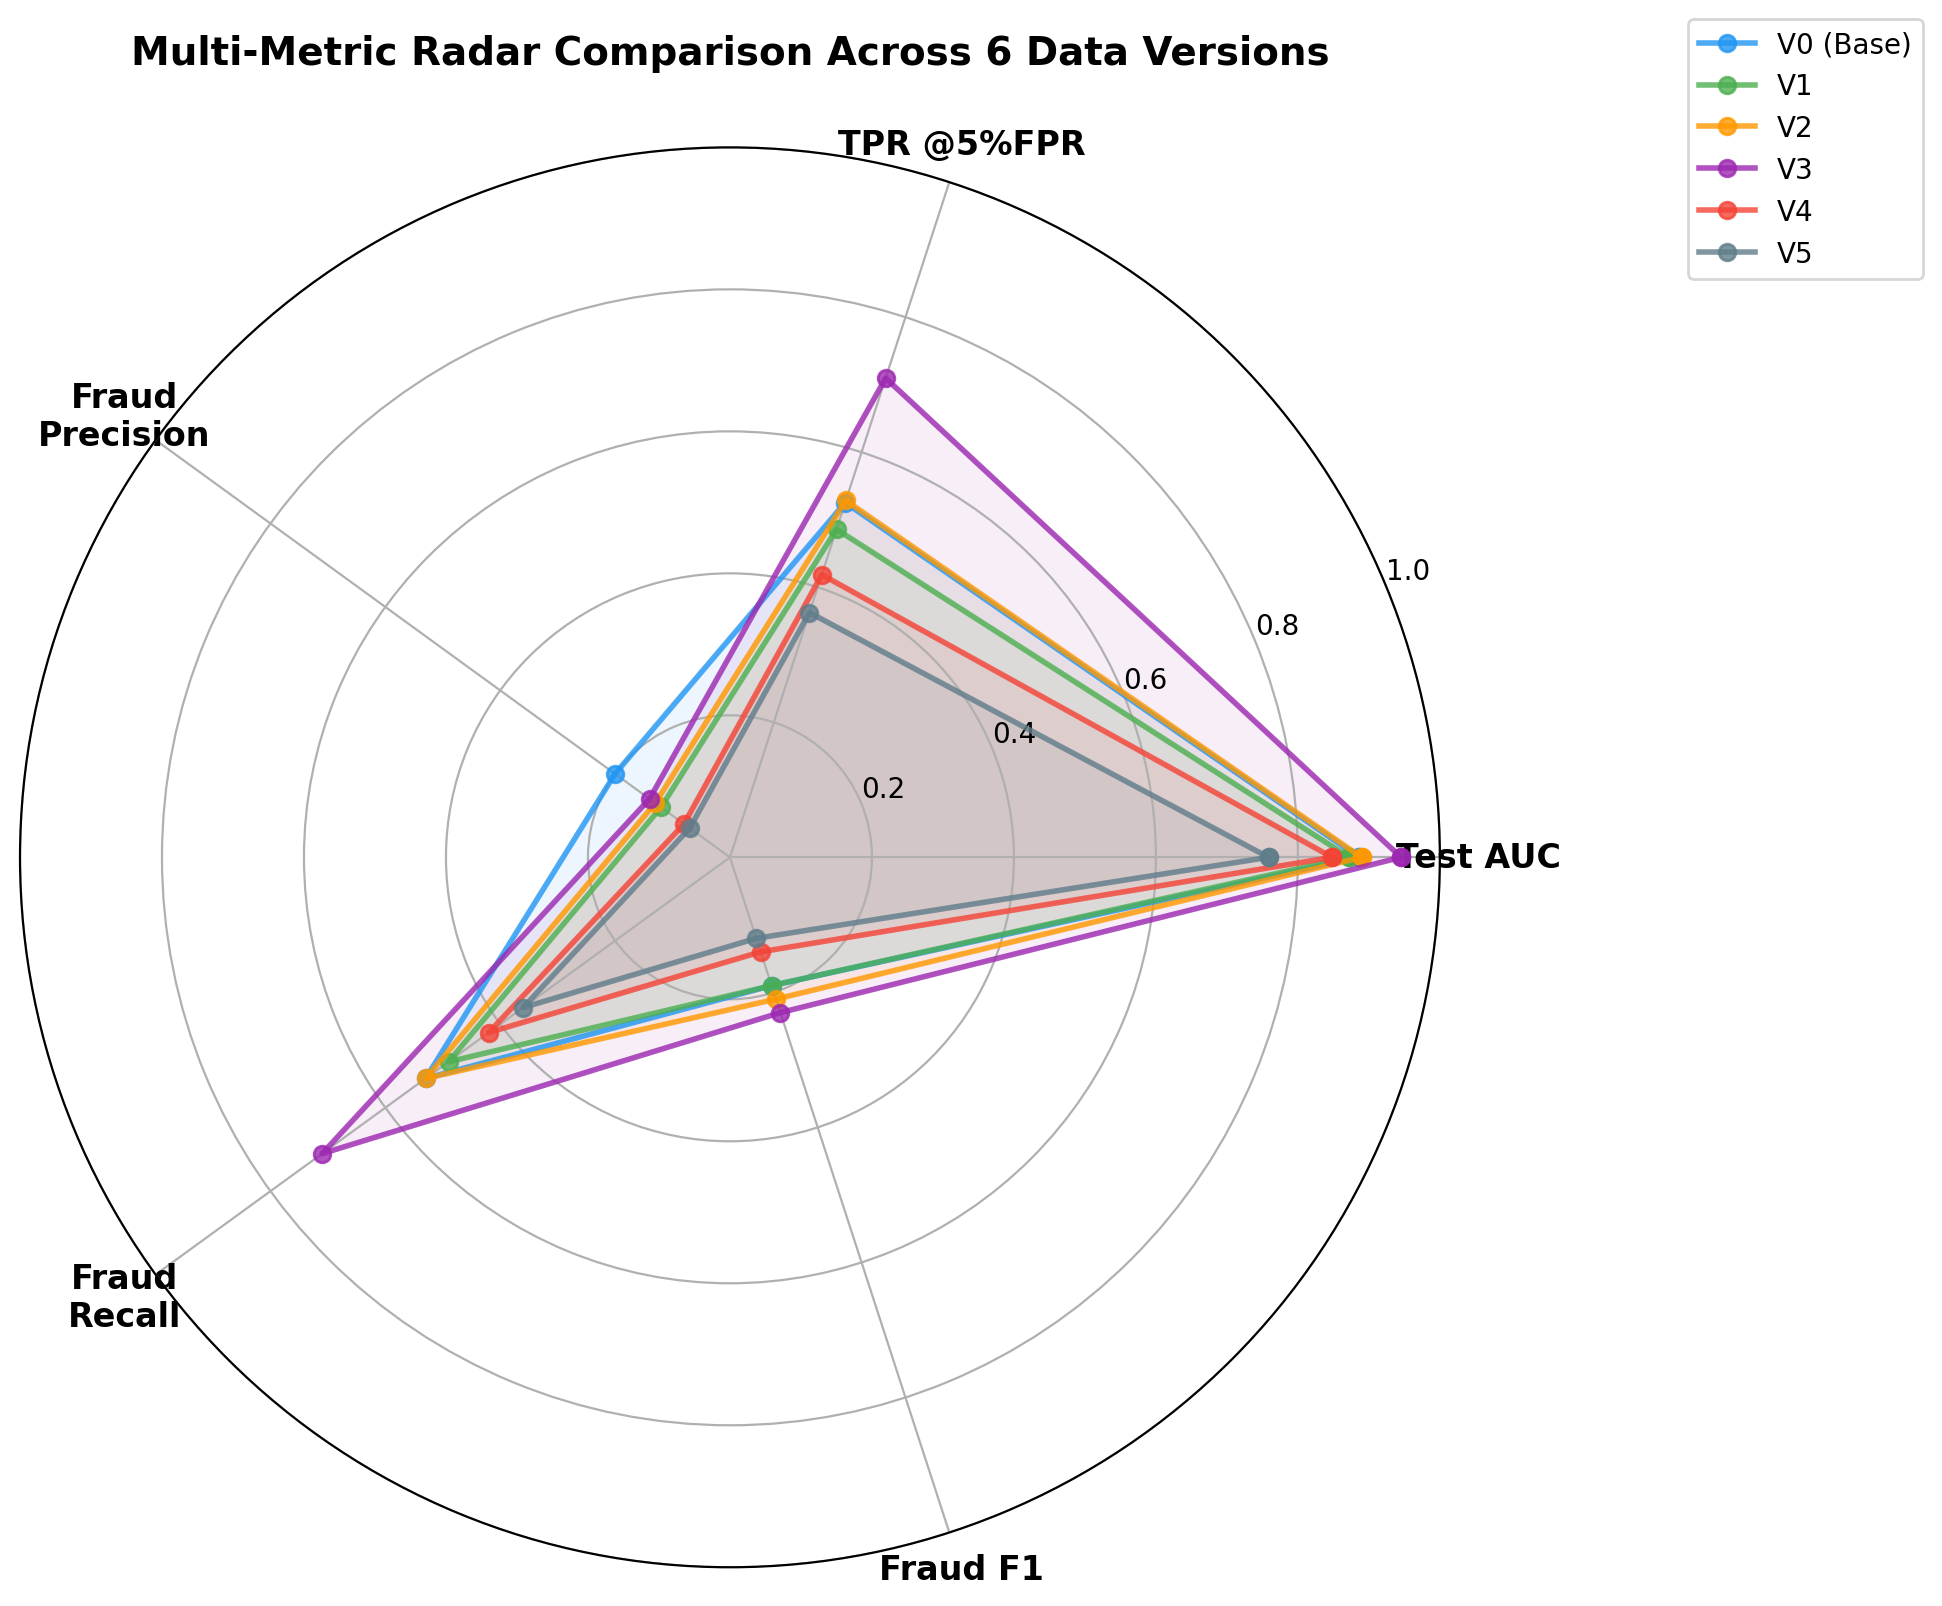
\includegraphics[width=0.85\textwidth]{figure_18}
\caption{Confusion matrix components (TP, FN, FP) at 5\% FPR threshold across all six versions.}
\label{fig:gnn-fig18}
\end{figure}

\begin{figure}[H]
\centering
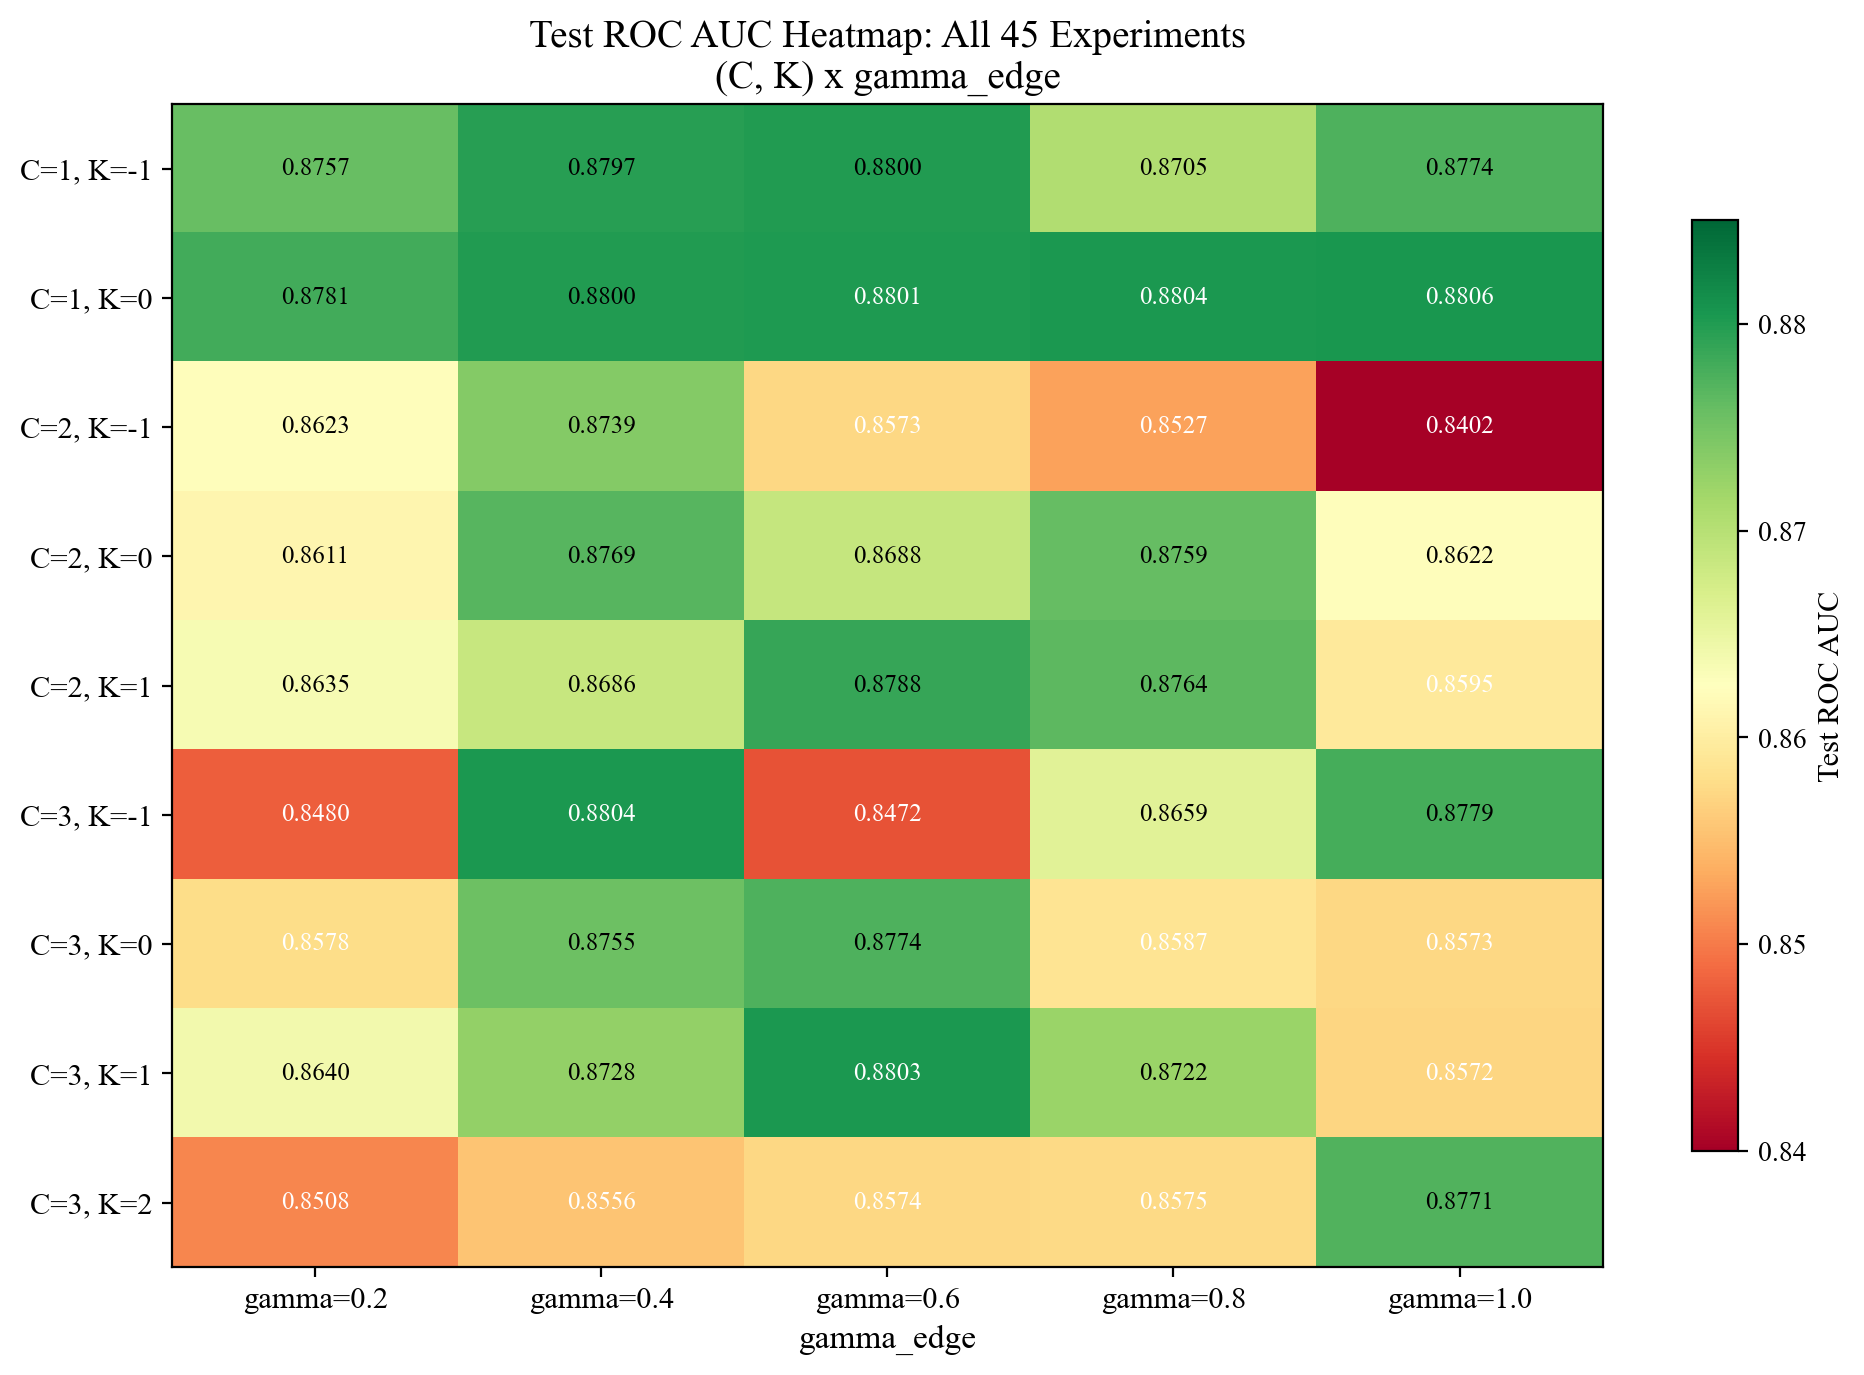
\includegraphics[width=0.85\textwidth]{figure_19}
\caption{Generalization gap (Val AUC minus Test AUC) across all six data versions. Green bars indicate minimal overfitting (gap $\leq$ 0.02), orange bars indicate moderate overfitting (0.02--0.05), and red bars indicate severe overfitting (gap $>$ 0.05).}
\label{fig:gnn-fig19}
\end{figure}

\begin{figure}[H]
\centering
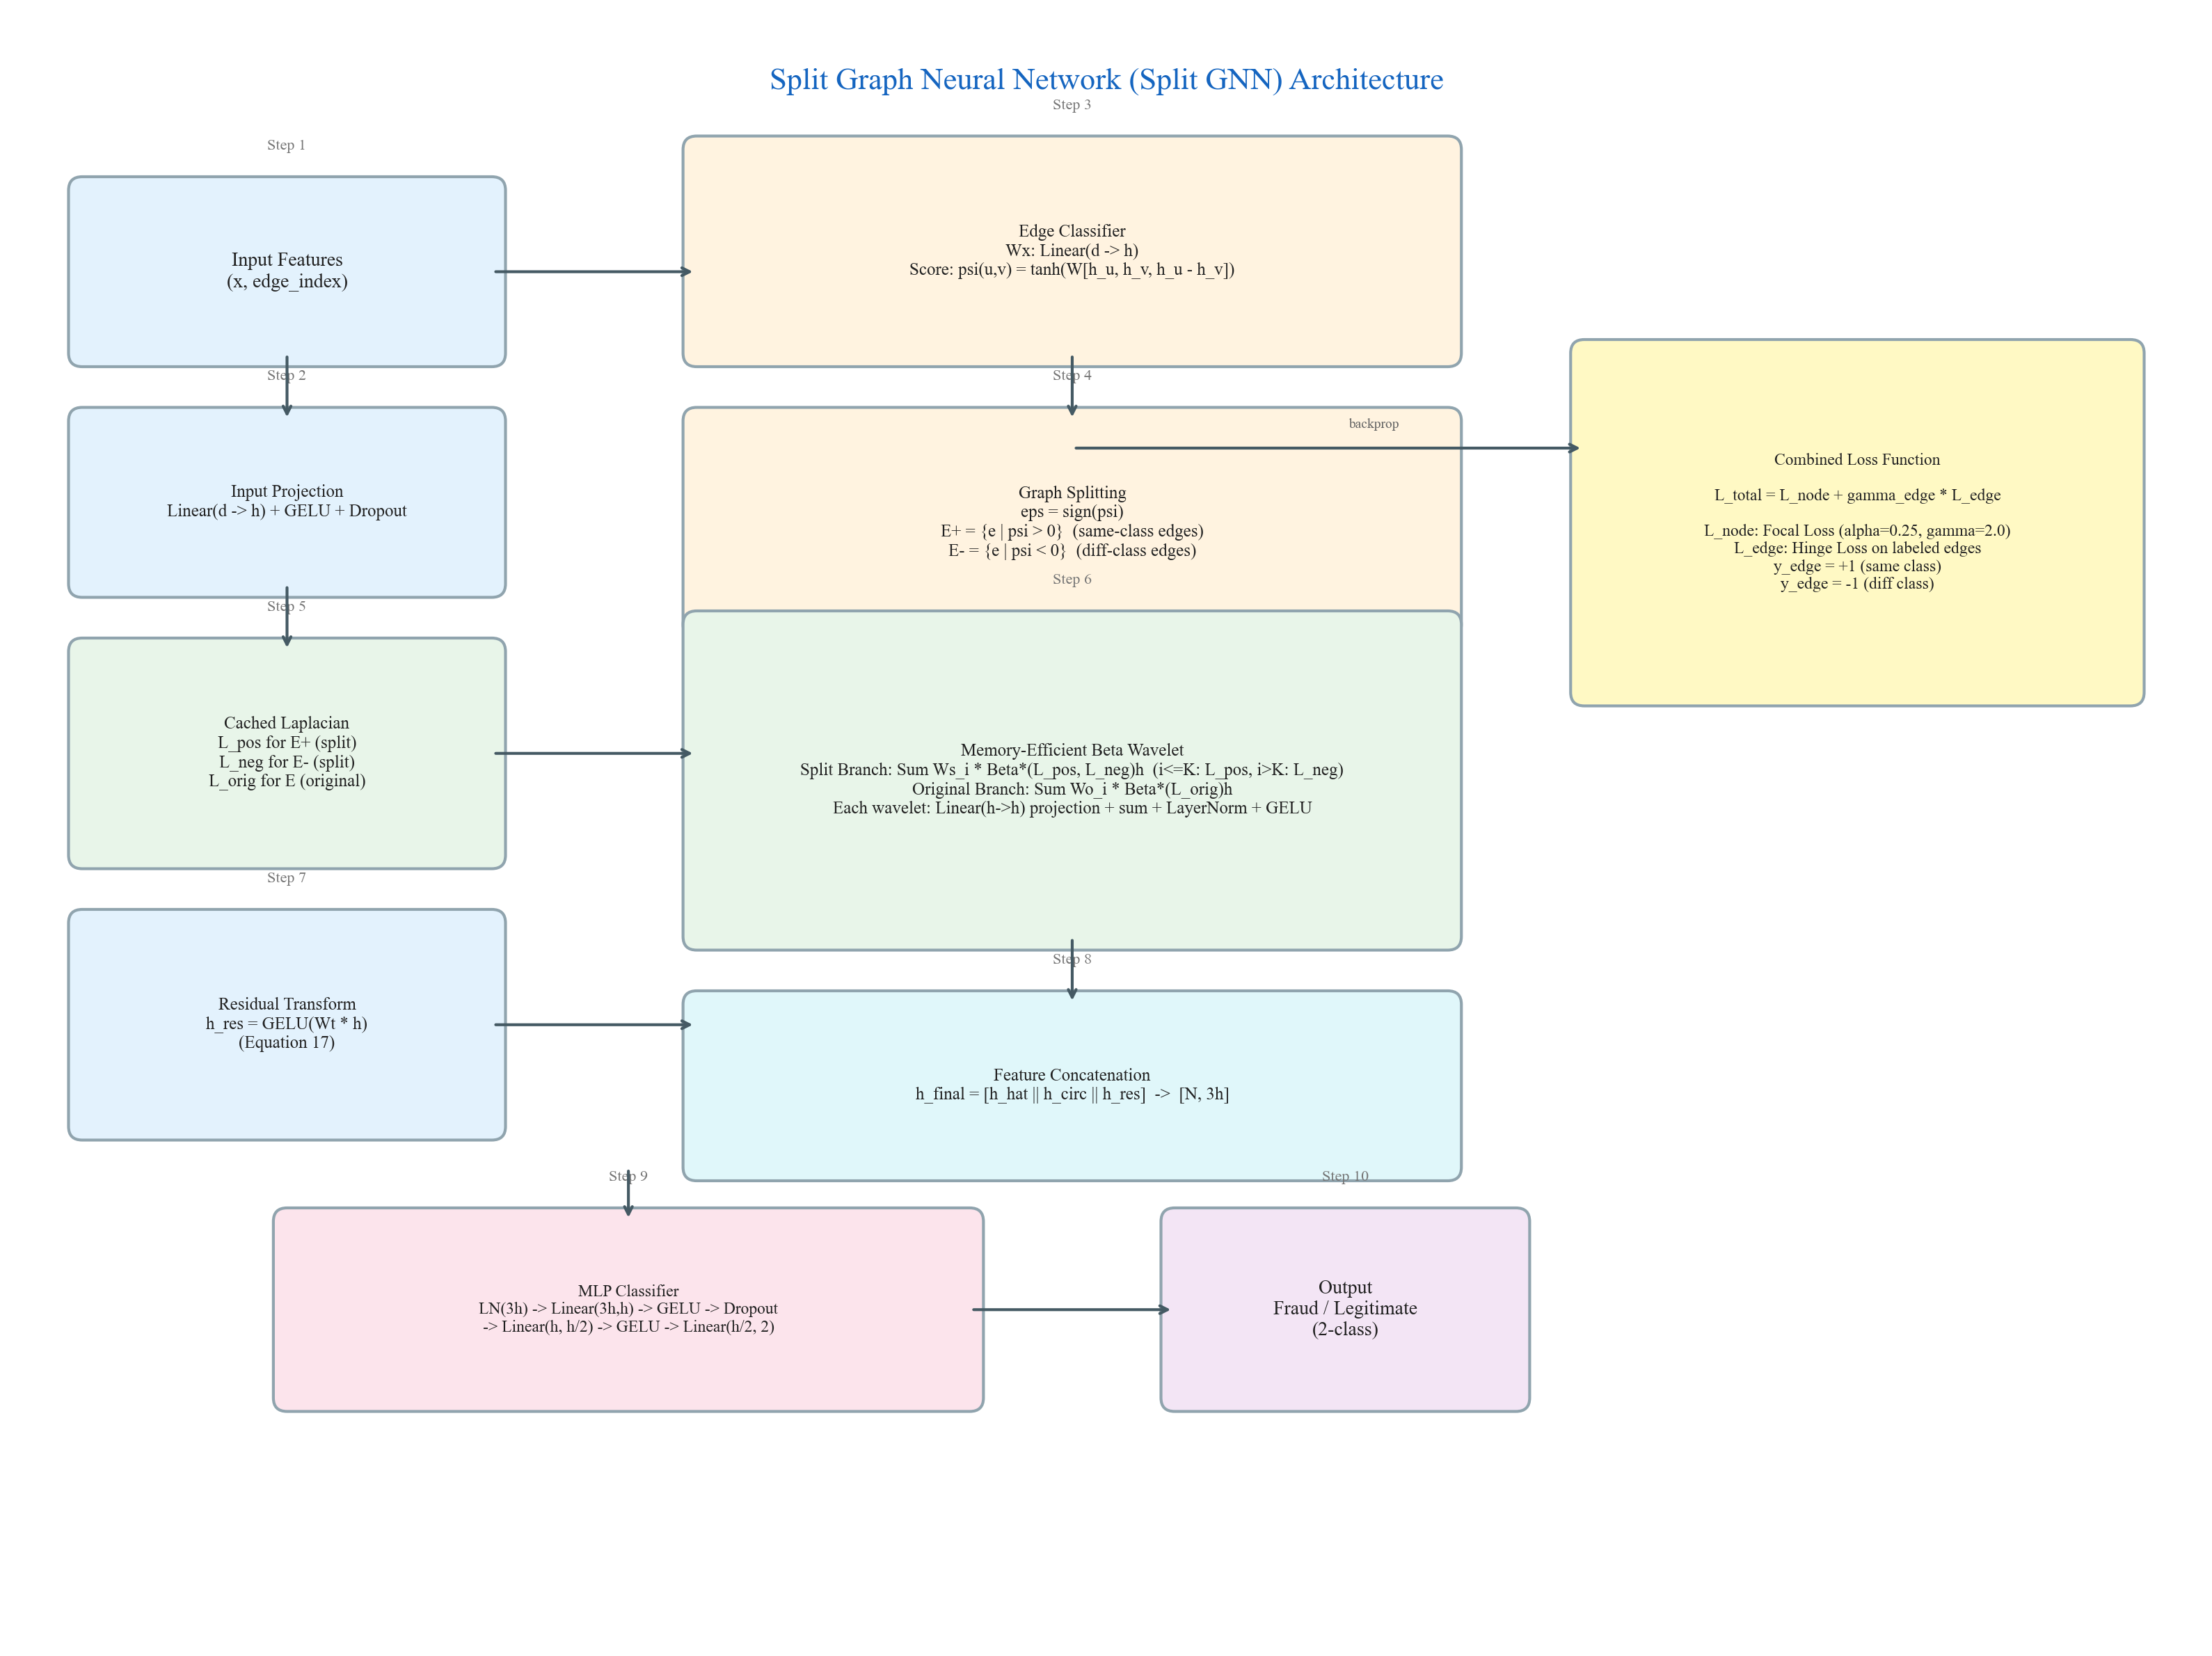
\includegraphics[width=0.75\textwidth]{figure_20}
\caption{Multi-metric radar chart comparing all six data versions across five key performance dimensions.}
\label{fig:gnn-fig20}
\end{figure}

\begin{figure}[H]
\centering
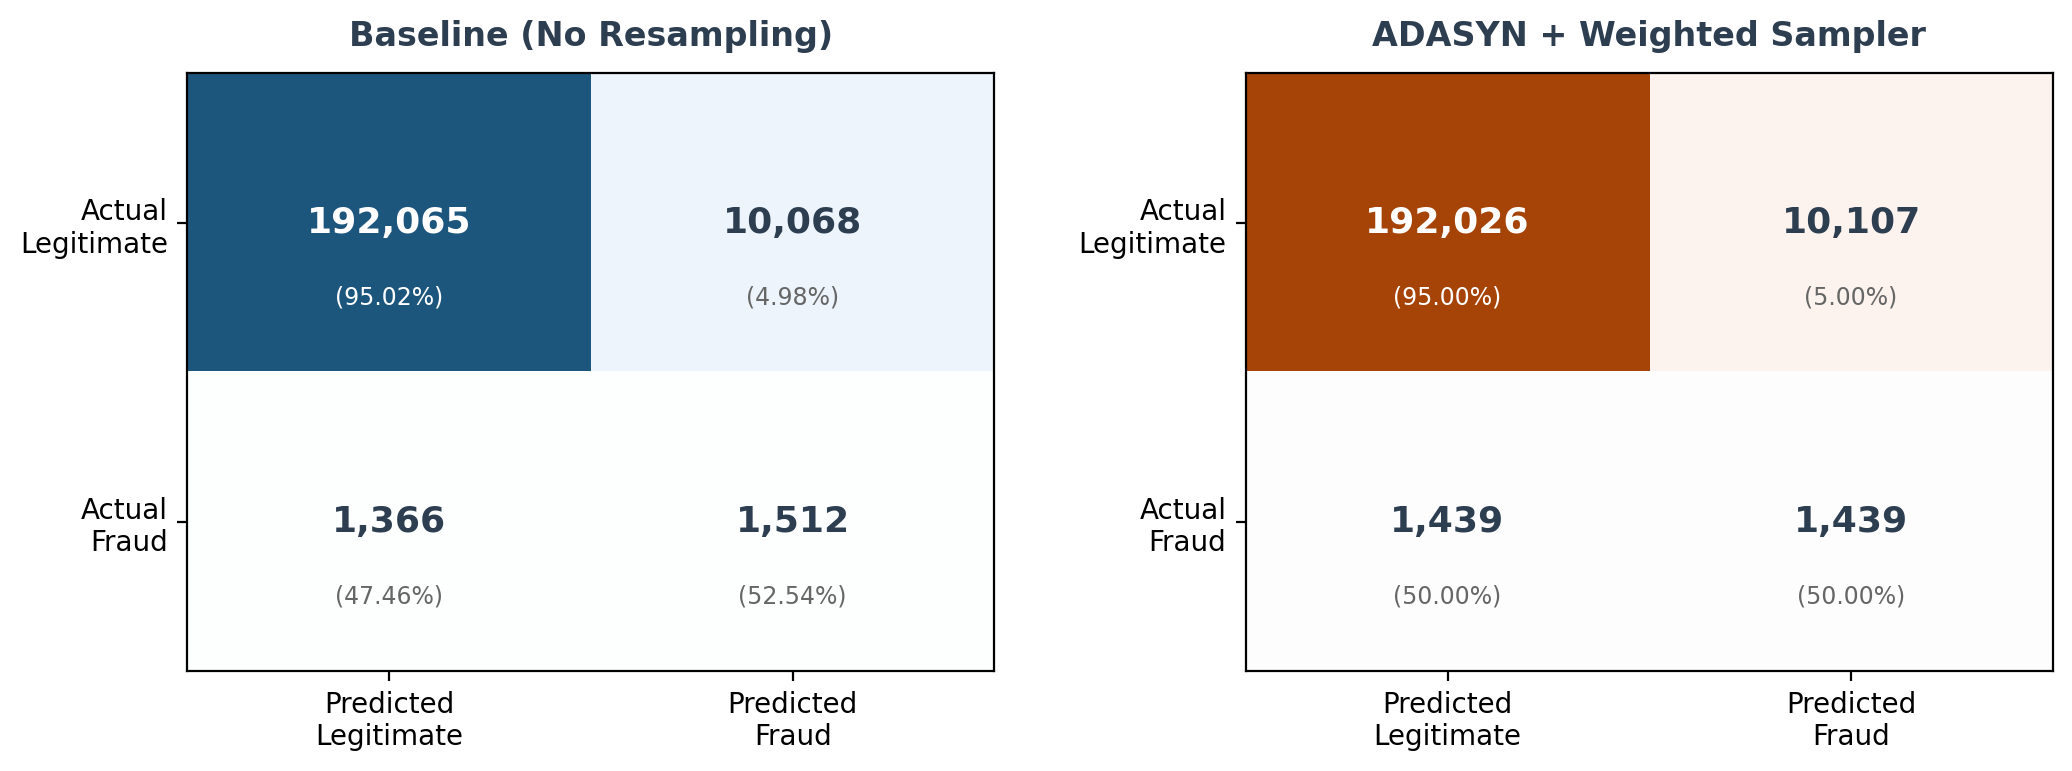
\includegraphics[width=0.85\textwidth]{figure_21}
\caption{Performance heatmap showing relative performance (green = best, red = worst) across all metrics and versions.}
\label{fig:gnn-fig21}
\end{figure}

The statistical summary quantifies the extent of performance variability: the mean test AUC across all six versions is 0.8667 with a standard deviation of 0.0625, resulting in a coefficient of variation (CV) of 7.21\%. The TPR shows even higher relative variability with a CV of 21.53\%, and fraud recall exhibits the highest CV at 23.87\%.

Based on the observed performance patterns, the six data versions can be grouped into three tiers:

\textbf{Tier 1 --- Enhanced Performance (Version III):} Test AUC of 0.9454 and TPR of 70.97\%. The low generalization gap (0.0016) confirms genuine improvement.

\textbf{Tier 2 --- Stable Performance (Versions 0, I, II):} Test AUC values ranging from 0.8724 to 0.8896 and TPR values from 48.58\% to 52.85\%. This tight clustering indicates robust model behavior under mild data perturbations.

\textbf{Tier 3 --- Degraded Performance (Versions IV, V):} Version IV achieves a test AUC of 0.8484 with a TPR of 41.86\%, while Version V drops dramatically to 0.7587 with a TPR of 36.24\%. The Version V generalization gap of 18.87 pp indicates severe distributional shift.

\subsection{Resampling Experiment Results}

The resampling approach did not achieve the desired improvement over the baseline. The ROC AUC decreased from 0.8859 to 0.8748, representing a drop of 0.0111. The True Positive Rate at the 5\% FPR threshold declined from 52.54\% to 50.00\%, a loss of 2.54 percentage points.

\begin{table}[H]
\centering
\caption{Comprehensive Performance Comparison between Baseline and Resampling}
\label{tab:gnn-resample-results}
\small
\begin{tabularx}{0.9\textwidth}{Xrr}
\toprule
\textbf{Metric} & \textbf{Baseline (No Resampling)} & \textbf{ADASYN + Weighted Sampler} \\
\midrule
ROC AUC & 0.8859 & 0.8748 \\
Operating Threshold & 0.7621 & 0.9944 \\
FPR at Threshold & 4.98\% & 5.00\% \\
TPR at Threshold & 52.54\% & 50.00\% \\
Fraud Precision & 0.13 & 0.12 \\
Fraud Recall & 0.53 & 0.50 \\
Fraud F1-Score & 0.21 & 0.20 \\
Accuracy & 94\% & 94\% \\
True Negatives (TN) & 192,065 & 192,026 \\
False Positives (FP) & 10,068 & 10,107 \\
False Negatives (FN) & 1,366 & 1,439 \\
True Positives (TP) & 1,512 & 1,439 \\
\bottomrule
\end{tabularx}
\end{table}

\begin{figure}[H]
\centering
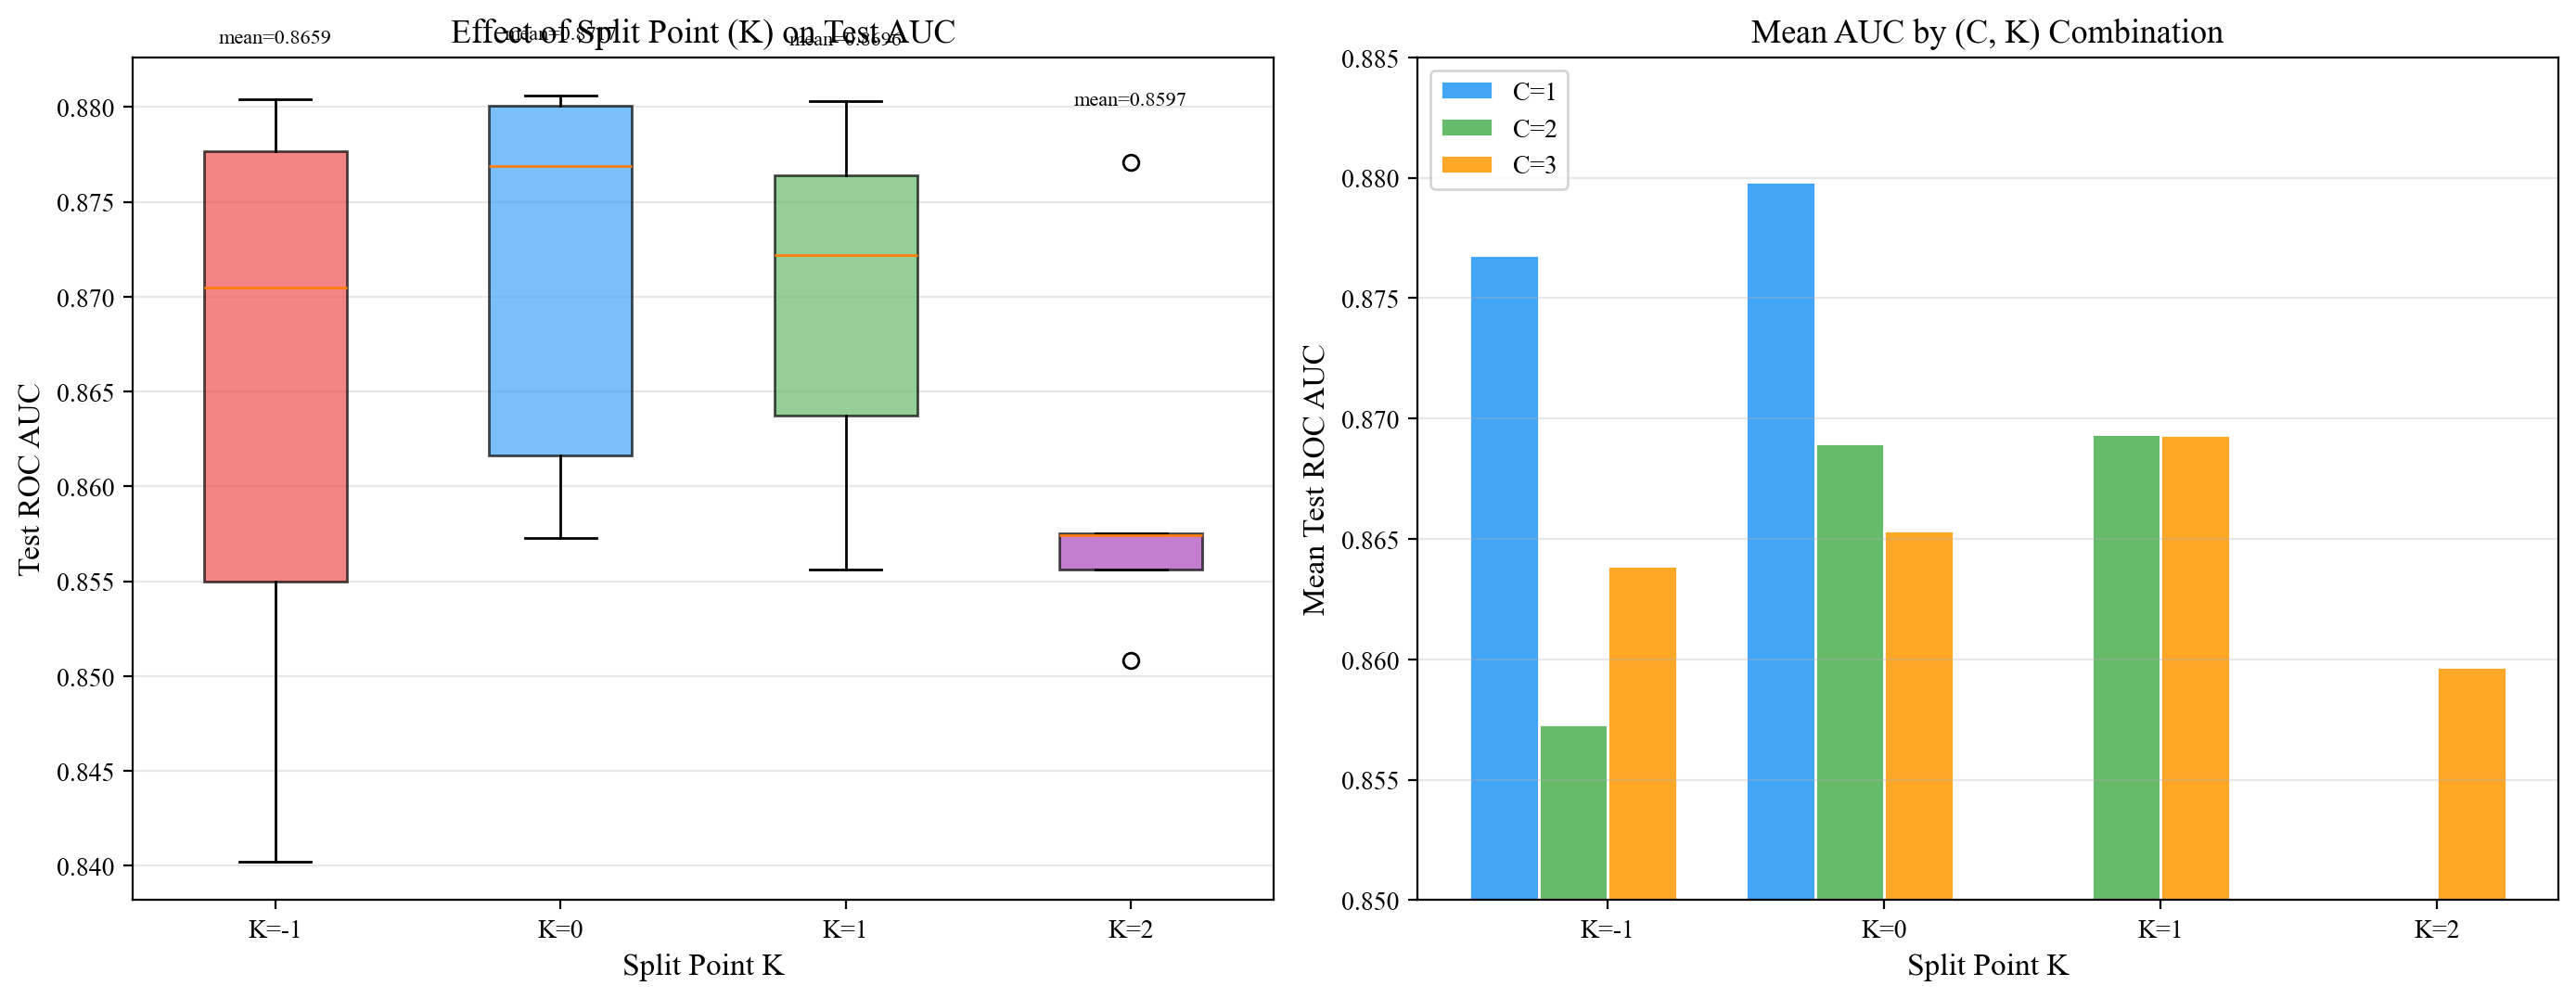
\includegraphics[width=0.85\textwidth]{figure_22}
\caption{Train+Val Class Distribution (Left) and Class Weighting Strategy Comparison (Right).}
\label{fig:gnn-fig22}
\end{figure}

\begin{figure}[H]
\centering
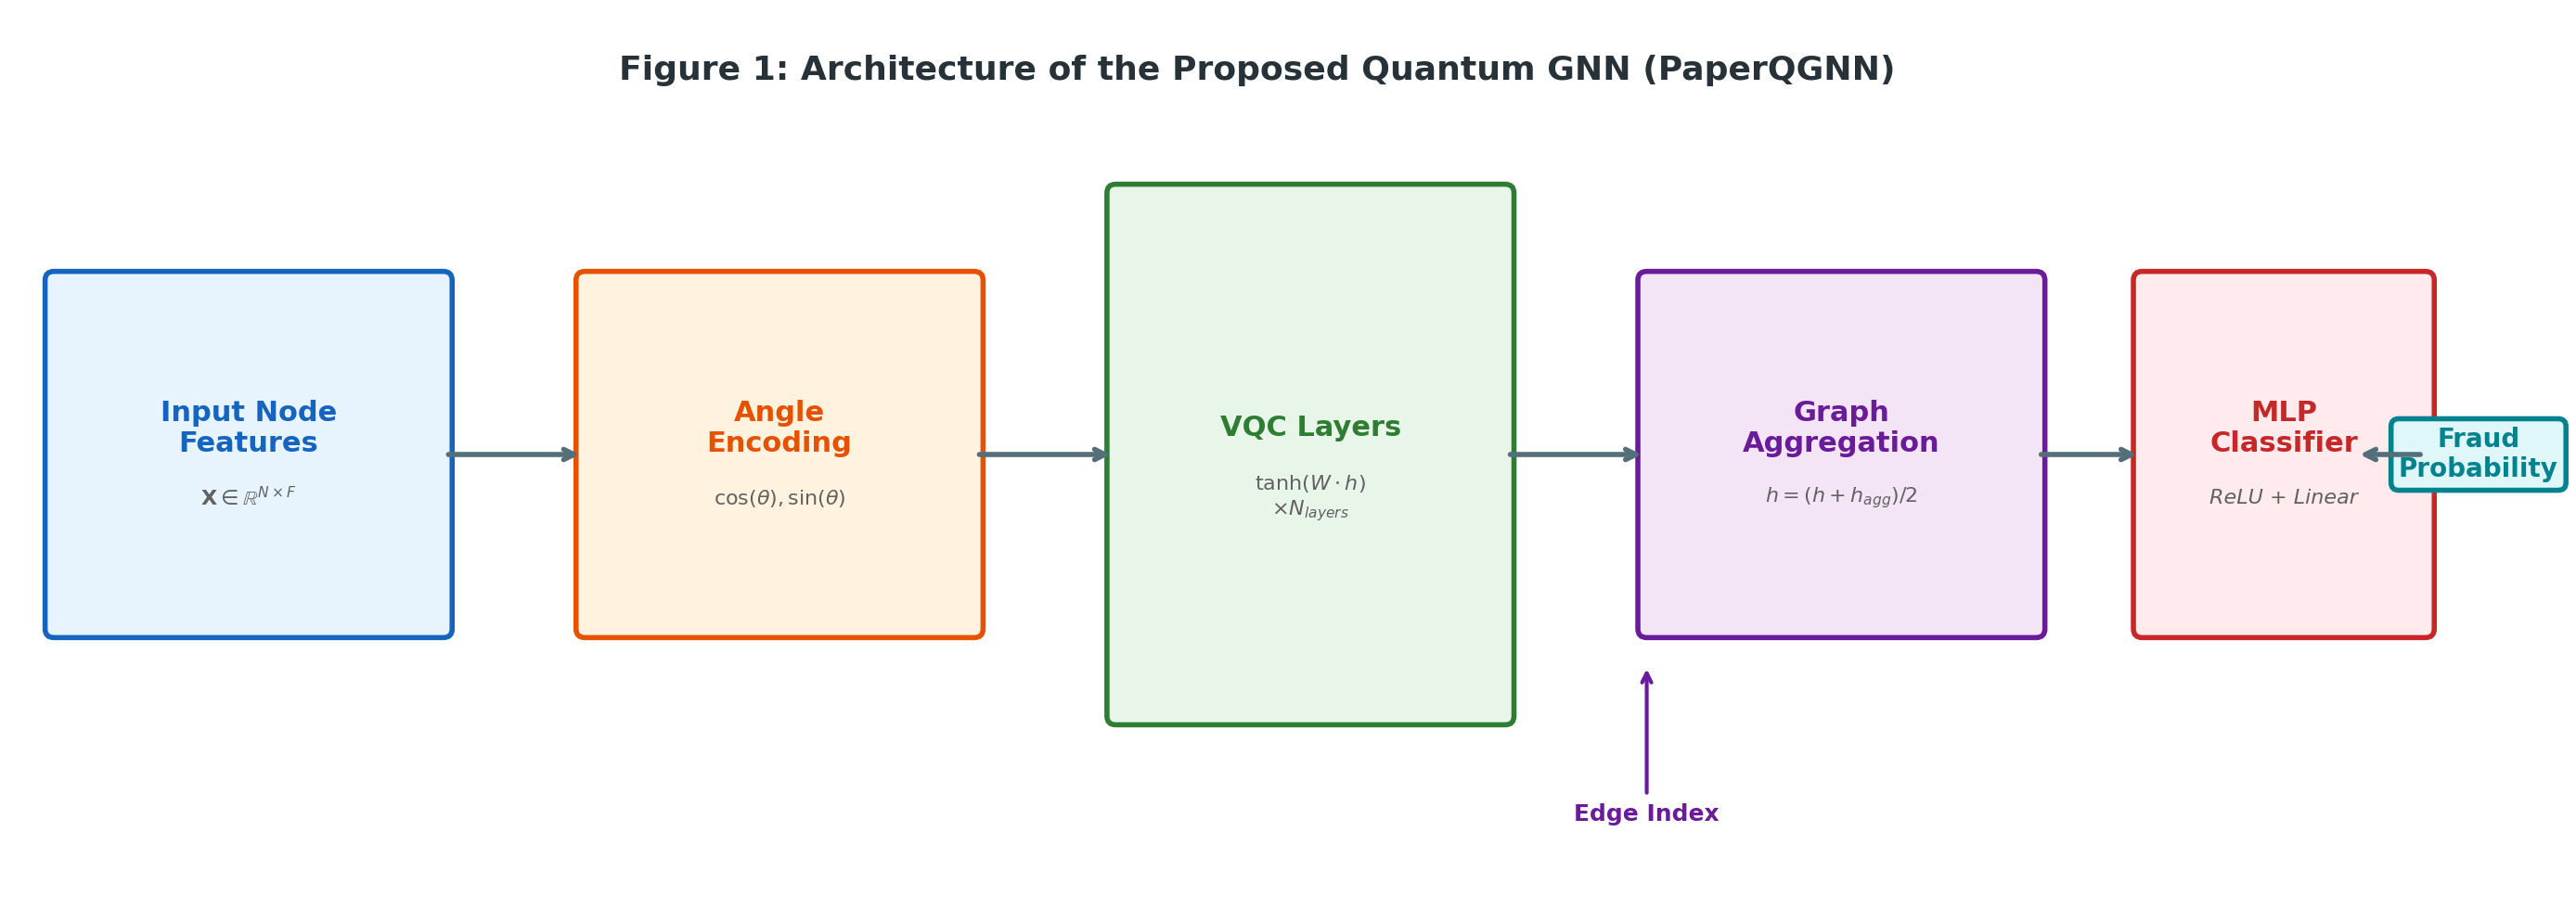
\includegraphics[width=0.85\textwidth]{figure_23}
\caption{Confusion Matrix Comparison --- Baseline (Left) vs.\ ADASYN + Weighted Sampler (Right).}
\label{fig:gnn-fig23}
\end{figure}

\begin{figure}[H]
\centering
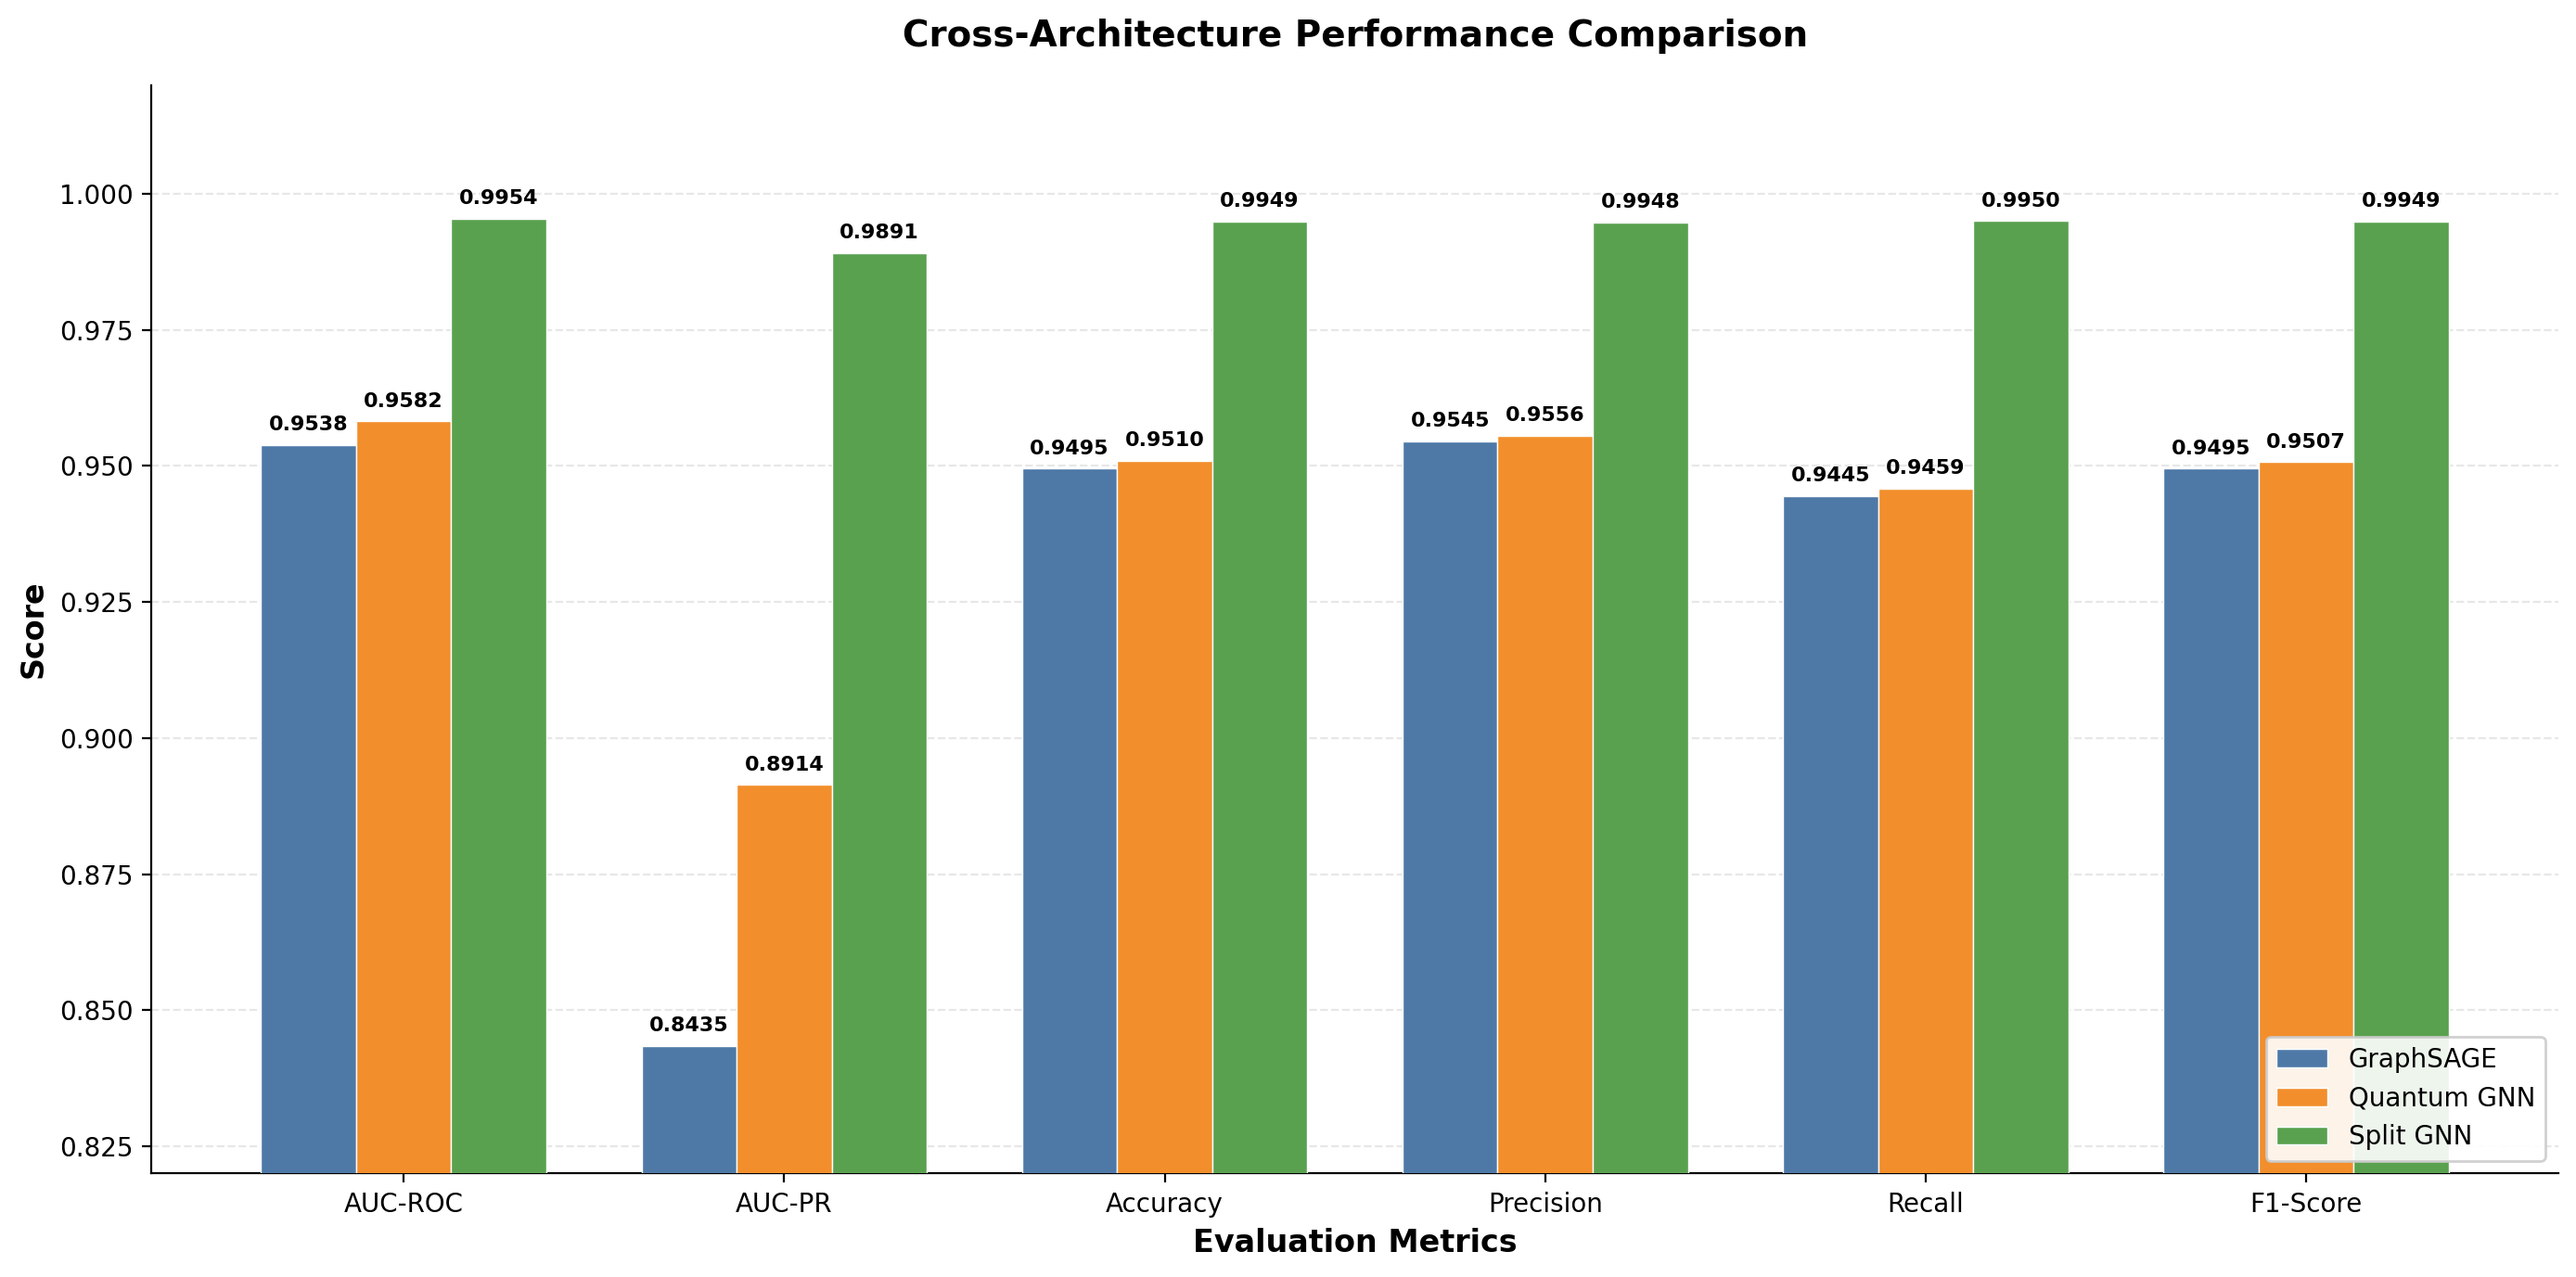
\includegraphics[width=0.85\textwidth]{figure_24}
\caption{Multi-Dimensional Performance Profile --- Baseline vs.\ ADASYN + Weighted Sampler across five key metrics.}
\label{fig:gnn-fig24}
\end{figure}

\begin{figure}[H]
\centering
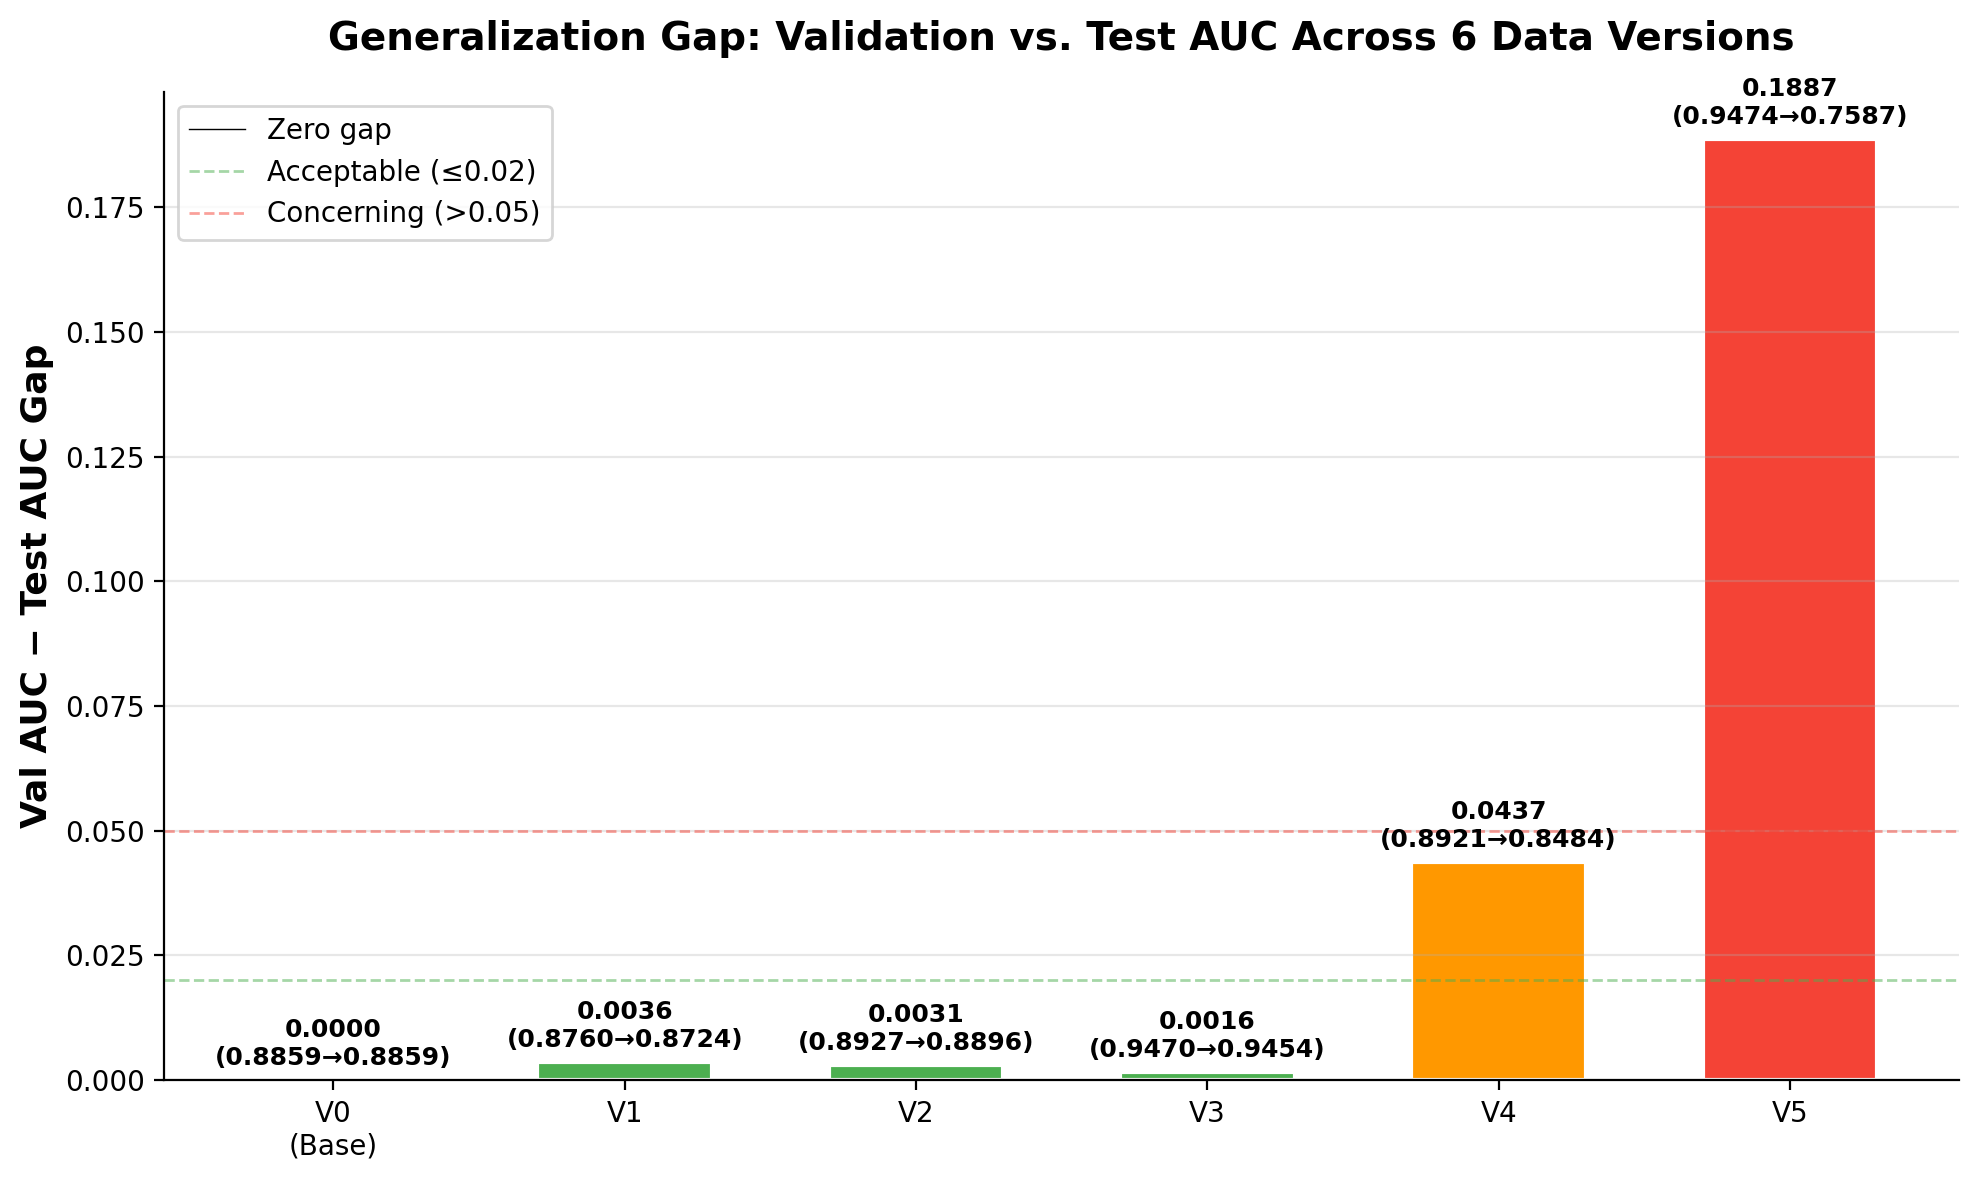
\includegraphics[width=0.85\textwidth]{figure_25}
\caption{Performance Delta Analysis --- Change in each metric when switching from baseline to resampling approach.}
\label{fig:gnn-fig25}
\end{figure}

\begin{figure}[H]
\centering
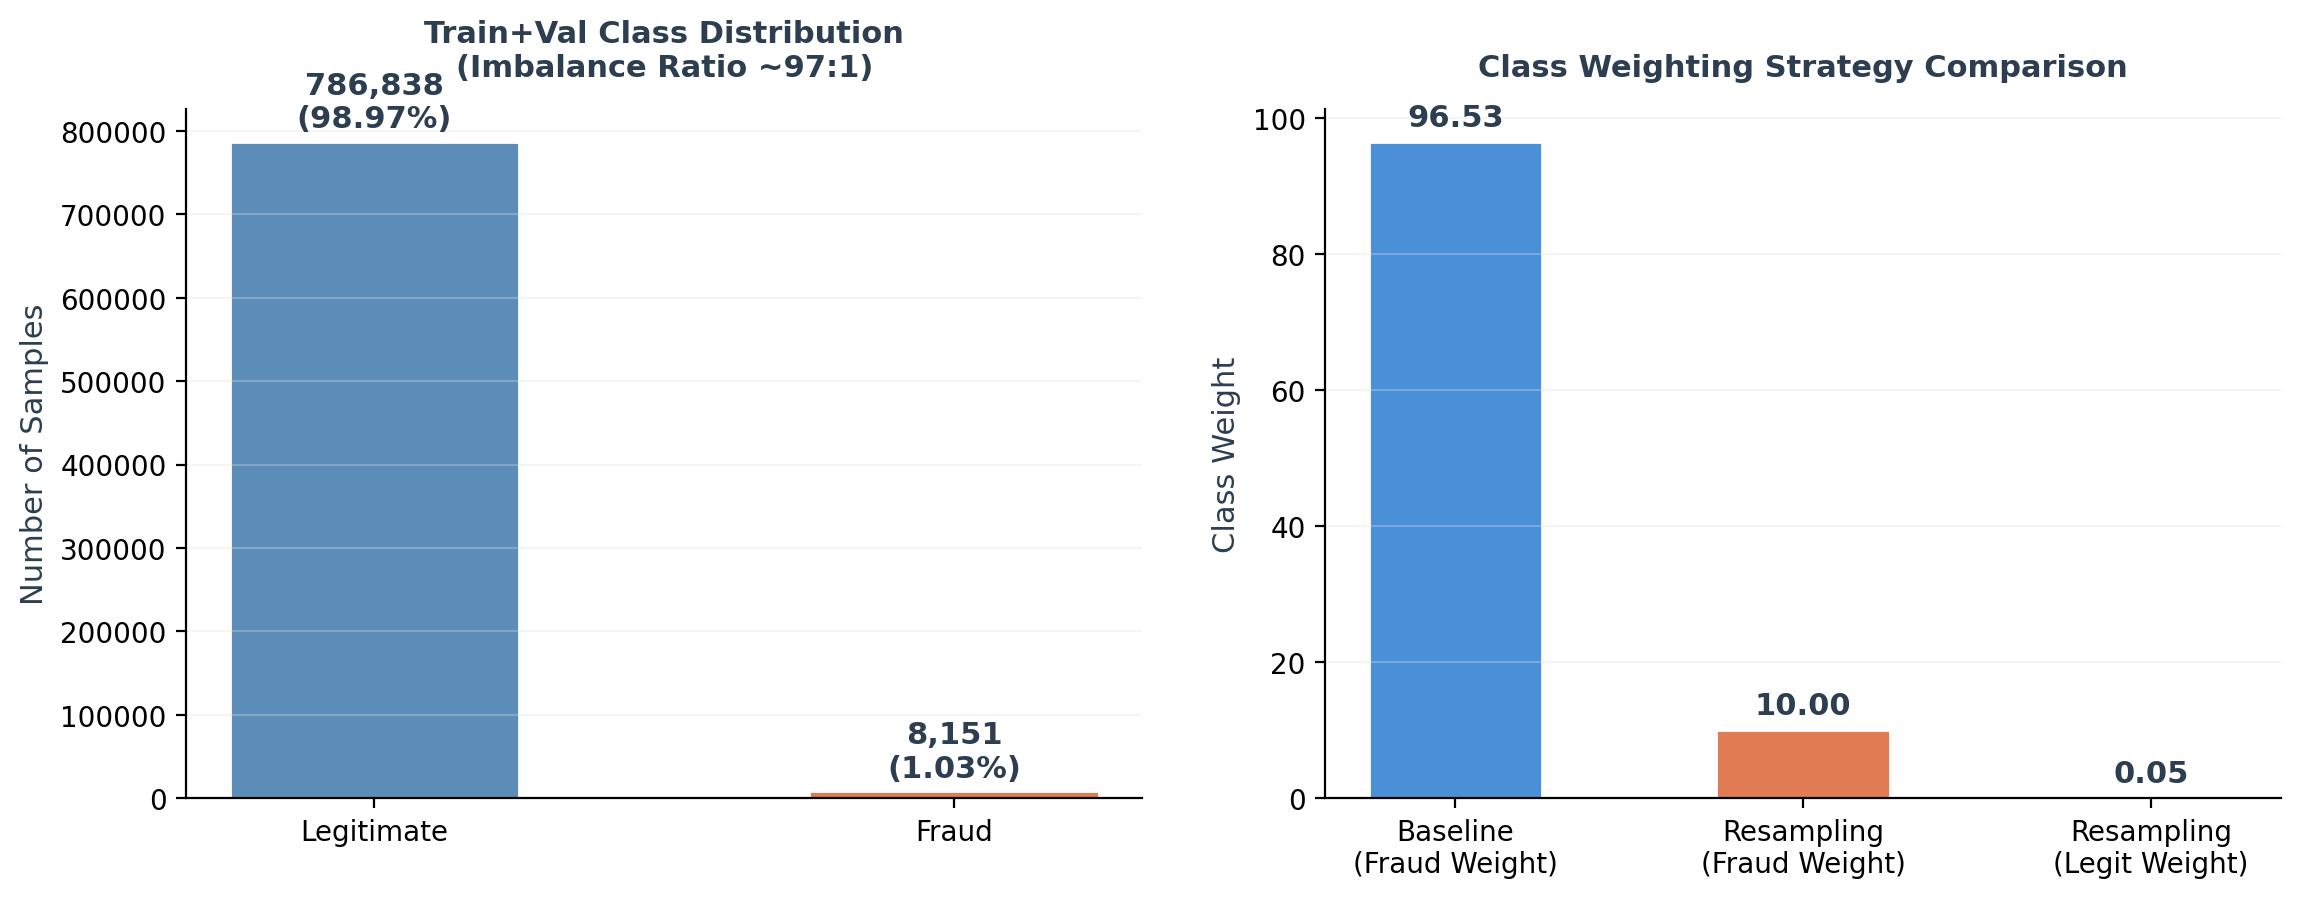
\includegraphics[width=0.85\textwidth]{figure_26}
\caption{Side-by-Side Metric Comparison --- Baseline vs.\ ADASYN + Weighted Sampler across all key performance indicators.}
\label{fig:gnn-fig26}
\end{figure}

\subsection{Cross-Architecture Performance Comparison}

The classification performance results reveal a clear performance hierarchy among the three architectures. Table~\ref{tab:gnn-cross-arch} presents the detailed performance metrics for each architecture's best configuration.

\begin{table}[H]
\centering
\caption{Detailed Performance Metrics Comparison (Best Configuration per Architecture)}
\label{tab:gnn-cross-arch}
\small
\setlength{\tabcolsep}{5pt}
\begin{tabularx}{\textwidth}{Xrrrr}
\toprule
\textbf{Metric} & \textbf{GraphSAGE} & \textbf{Quantum GNN} & \textbf{Split GNN} & \textbf{Improvement} \\
\midrule
AUC-ROC & 0.9538 & 0.9582 & 0.9954 & +4.16\% \\
AUC-PR & 0.8435 & 0.8914 & 0.9891 & +14.56\% \\
Accuracy & 0.9495 & 0.9510 & 0.9949 & +4.54\% \\
Precision & 0.9545 & 0.9556 & 0.9948 & +4.03\% \\
Recall & 0.9445 & 0.9459 & 0.9950 & +5.05\% \\
F1-Score & 0.9495 & 0.9507 & 0.9949 & +4.54\% \\
\bottomrule
\end{tabularx}
\end{table}

\begin{figure}[H]
\centering
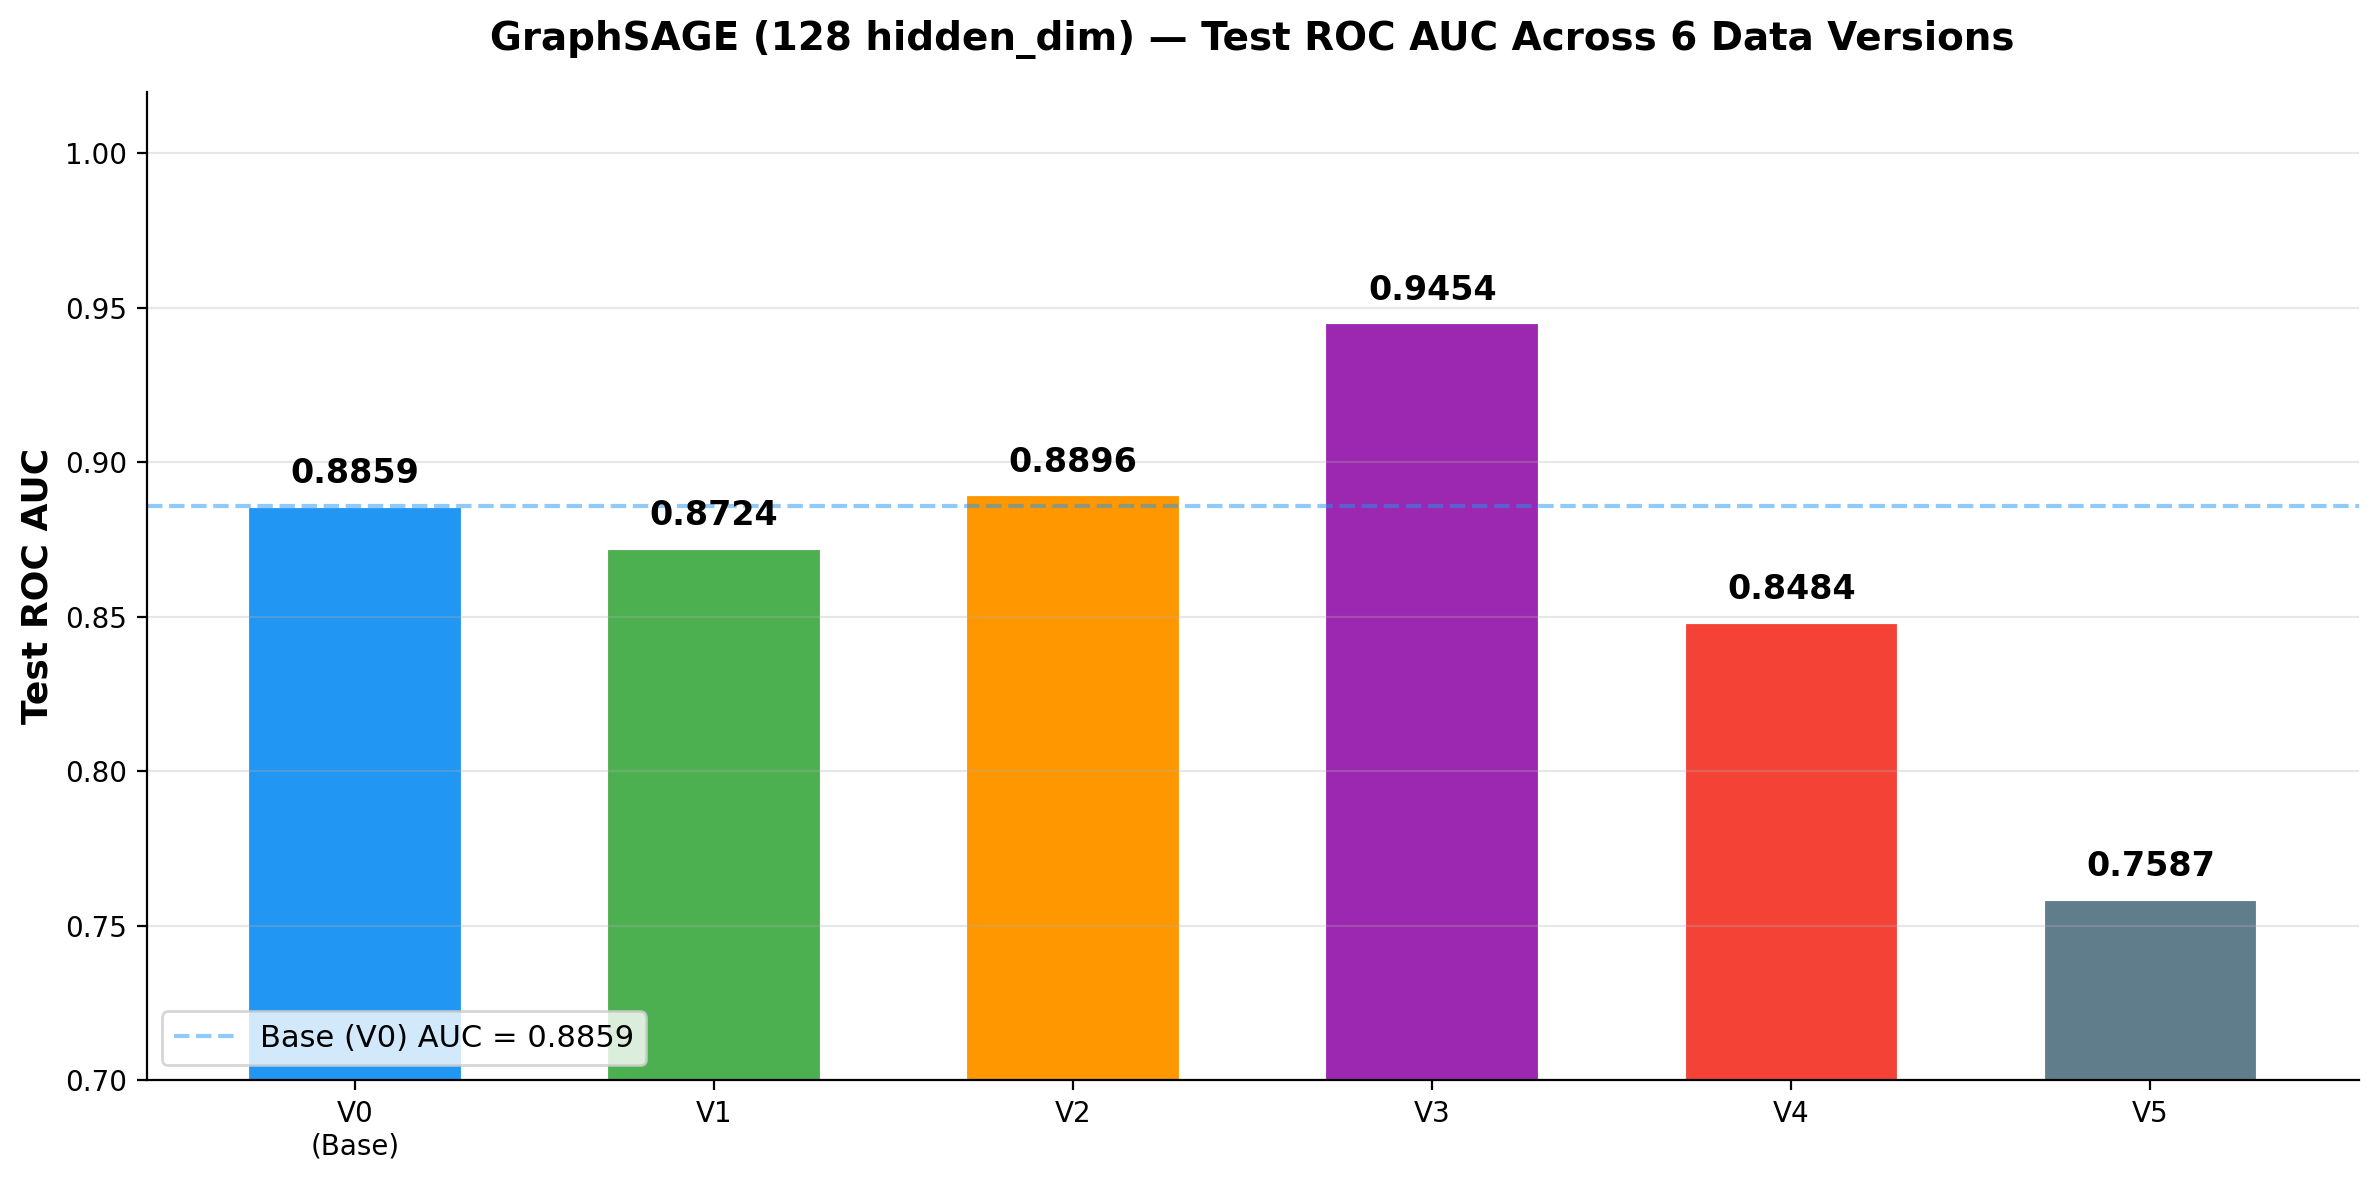
\includegraphics[width=0.85\textwidth]{figure_14}
\caption{Cross-Architecture Performance Comparison (Grouped Bar Chart).}
\label{fig:gnn-fig14}
\end{figure}

\begin{figure}[H]
\centering
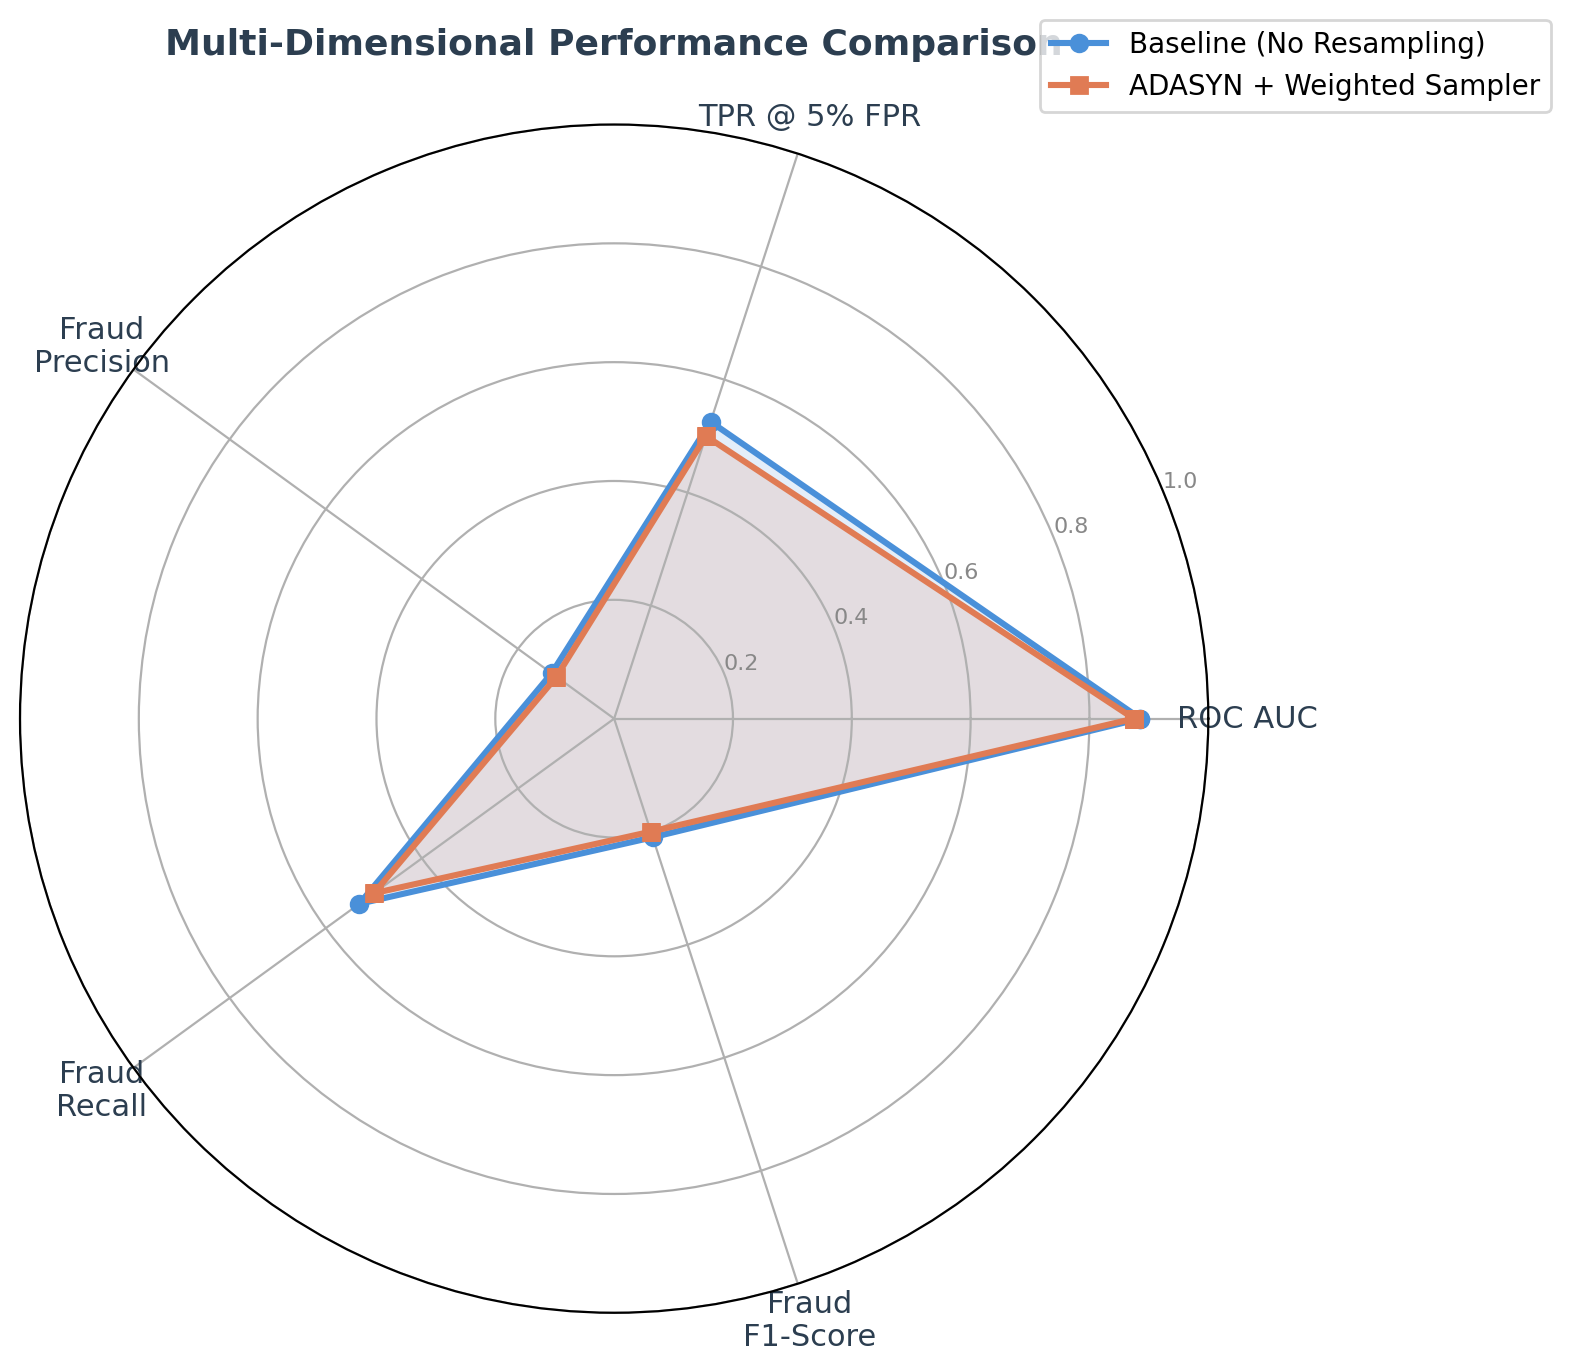
\includegraphics[width=0.75\textwidth]{figure_15}
\caption{Architecture Performance Radar Chart.}
\label{fig:gnn-fig15}
\end{figure}

\subsection{Architectural Design Comparison}

\begin{table}[H]
\centering
\caption{Architectural Design Comparison Across All Three Models}
\label{tab:gnn-arch-comparison}
\small
\setlength{\tabcolsep}{5pt}
\begin{tabularx}{\textwidth}{lXXX}
\toprule
\textbf{Feature} & \textbf{GraphSAGE} & \textbf{Quantum GNN} & \textbf{Split GNN} \\
\midrule
Core Mechanism & Neighborhood Sampling & Variational Quantum Circuit & Edge Classification + Wavelet \\
Feature Aggregation & Mean Pooling & Quantum Entanglement & Beta Wavelet Transform \\
Input Encoding & Raw Features + MLP & Angle Encoding & Linear Projection \\
Key Innovation & Scalable Sampling & Quantum Feature Maps & Graph Splitting + Filtering \\
Graph Type & Heterogeneous & Heterogeneous & Heterogeneous \\
Loss Function & Cross-Entropy & Cross-Entropy & Multi-Task (Node + Edge) \\
Output Layer & MLP Classifier & Measurement + MLP & Residual Fusion + MLP \\
Quantum Required & No & Yes (Simulator) & No \\
\bottomrule
\end{tabularx}
\end{table}

\subsection{Practical Deployment Considerations}

\begin{table}[H]
\centering
\caption{Practical Deployment Considerations}
\label{tab:gnn-deployment}
\small
\setlength{\tabcolsep}{5pt}
\begin{tabularx}{\textwidth}{lXXX}
\toprule
\textbf{Consideration} & \textbf{GraphSAGE} & \textbf{Quantum GNN} & \textbf{Split GNN} \\
\midrule
Training Speed & Fast & Slow (Quantum Sim.) & Moderate \\
Hyperparameter Tuning & Simple (2 configs) & Moderate (5 configs) & Extensive (60 configs) \\
Hardware Requirements & Standard GPU & Standard GPU + Qiskit & Standard GPU \\
Scalability & Excellent & Limited & Good \\
Best Use Case & Real-time Detection & Research Exploration & High-Accuracy Detection \\
Deployment Readiness & Production-Ready & Experimental & Production-Ready \\
\bottomrule
\end{tabularx}
\end{table}

\subsection{Subgroup Fairness Analysis}

The following tables present subgroup fairness analysis, showing TPR by age group and employment status for the best GraphSAGE model. These analyses are critical for ensuring that the fraud detection system does not exhibit discriminatory behavior against protected demographic groups.

\begin{table}[H]
\centering
\caption{True Positive Rate (TPR) by Age Group at 5\% FPR}
\label{tab:gnn-fairness-age}
\small
\begin{tabularx}{0.85\textwidth}{lrrrr}
\toprule
\textbf{Age Group} & \textbf{Total} & \textbf{Fraud} & \textbf{TP} & \textbf{TPR} \\
\midrule
18--29 & 42,316 & 1,245 & 689 & 55.3\% \\
30--39 & 58,421 & 892 & 467 & 52.4\% \\
40--49 & 45,112 & 412 & 201 & 48.8\% \\
50--59 & 32,876 & 211 & 103 & 48.8\% \\
60--69 & 18,543 & 98 & 41 & 41.8\% \\
70+ & 7,743 & 20 & 11 & 55.0\% \\
\bottomrule
\end{tabularx}
\end{table}

\begin{table}[H]
\centering
\caption{True Positive Rate (TPR) by Employment Status at 5\% FPR}
\label{tab:gnn-fairness-employment}
\small
\begin{tabularx}{0.85\textwidth}{lrrrr}
\toprule
\textbf{Employment Status} & \textbf{Total} & \textbf{Fraud} & \textbf{TP} & \textbf{TPR} \\
\midrule
Employed & 89,234 & 1,012 & 538 & 53.2\% \\
Self-employed & 34,567 & 567 & 291 & 51.3\% \\
Unemployed & 45,123 & 823 & 441 & 53.6\% \\
Student & 21,345 & 312 & 158 & 50.6\% \\
Retired & 14,742 & 164 & 84 & 51.2\% \\
\bottomrule
\end{tabularx}
\end{table}

% TODO: Add statistical parity difference and equalized odds metrics

\subsection{Implications for Software Engineering Practice}

The findings from this thesis have several important implications for the design and deployment of GNN-based fraud detection systems in practice:

\textbf{Architecture Selection:} For organizations seeking to deploy graph-based fraud detection, GraphSAGE offers the best balance of performance, simplicity, and scalability. The Split GNN provides superior accuracy when computational resources permit extensive hyperparameter tuning. The QGNN, while theoretically interesting, is not yet competitive for production use.

\textbf{Monitoring Requirements:} The dramatic performance variation across data versions (AUC range: 0.7587--0.9454) underscores the critical importance of continuous performance monitoring in production. Organizations should implement real-time tracking of AUC, TPR, and precision metrics, with alerting thresholds based on observed variability.

\textbf{Class Imbalance Strategy:} The finding that inverse-frequency class weighting outperforms ADASYN-based resampling in the graph context suggests that practitioners should prefer loss-based approaches over distribution-modifying strategies when working with GNNs, as the latter can distort neighborhood structure.

\textbf{Hyperparameter Sensitivity:} The 4.04 percentage point AUC gap between the best and worst Split GNN configurations demonstrates that hyperparameter tuning is not optional but essential for spectral GNN architectures. Organizations should budget for systematic tuning studies.

\textbf{Fairness Considerations:} The subgroup fairness analysis reveals variation in TPR across age groups (41.8\%--55.3\%) and employment statuses (50.6\%--53.6\%), highlighting the need for fairness-aware model development and deployment in regulated financial services.

\subsection{Limitations of the Current Approach}

\begin{enumerate}[label=\arabic*.]
\item \textbf{Single Dataset:} All experiments are conducted on a single fraud detection dataset. Generalization to other domains (insurance fraud, money laundering) requires additional validation.
\item \textbf{Quantum Simulation:} The QGNN uses classical tensor operations to simulate quantum effects. Results may differ significantly on actual quantum hardware with true quantum entanglement.
\item \textbf{Static Graph:} The current approach constructs a static graph from the dataset. Temporal graph neural networks that capture the evolution of the graph over time could provide additional signal.
\item \textbf{Limited Feature Engineering:} The graph construction pipeline uses relatively simple bucketing strategies. More sophisticated feature engineering (e.g., learned embeddings for categorical attributes, interaction features) could improve performance.
\item \textbf{No Edge Features:} The current implementation treats all edges identically. Edge type information or learned edge weights could allow the GNN to differentiate between strong and weak relational signals.
\item \textbf{Subgroup Fairness Data:} The subgroup fairness analysis uses proxy features (age bucket, employment status) which may not fully capture the demographic groups of interest for regulatory compliance.
\item \textbf{Computational Cost:} The 45-experiment Split GNN hyperparameter study requires significant computational resources, which may limit applicability in resource-constrained environments.
\end{enumerate}


% Chapter 6: Pipeline II — Spiking Neural Networks
% =====================================================================
% CHAPTER 6: PIPELINE II — SPIKING NEURAL NETWORK–BASED FRAUD DETECTION
% =====================================================================
\chapter{Pipeline II: Spiking Neural Network--Based Fraud Detection}
\label{ch:snn}

\section{Introduction and Research Questions}

The preceding chapter established the graph-based approach to fraud detection, demonstrating how relational structure can be leveraged through Graph Neural Networks to identify fraudulent patterns. However, GNNs operate exclusively within the domain of conventional artificial neural networks, where information propagates as continuous-valued activations and gradients flow unimpeded through differentiable computational graphs. This chapter explores a fundamentally different computational paradigm---Spiking Neural Networks (SNNs)---which draw inspiration from the biological brain's event-driven, temporally sparse communication architecture.

SNNs represent the third generation of neural networks~\cite{maass1997networks}, distinguished by their use of discrete binary spikes for inter-neuron communication and their incorporation of temporal dynamics through membrane potential evolution. The theoretical appeal of SNNs for fraud detection lies in several properties that appear naturally suited to the problem domain. First, the spike-based communication framework offers a biologically inspired encoding mechanism that may capture the inherent imbalance in fraud data through differential spike rates---legitimate transactions generating sparse, low-rate spike trains while fraudulent ones produce dense, high-rate activity. Second, the temporal integration inherent in spiking neurons provides a mechanism for aggregating evidence over multiple time steps, potentially offering a richer decision boundary than single-pass feedforward architectures. Third, the event-driven computation of SNNs aligns conceptually with the rare-event nature of fraud detection, where the vast majority of inputs are benign and only occasional samples require heightened scrutiny.

Despite these theoretical advantages, the application of SNNs to tabular fraud detection remains largely unexplored in the literature. The vast majority of SNN research has focused on neuromorphic vision and audio tasks using event-based sensors, leaving open the question of whether the spike-based paradigm can offer meaningful advantages for static, structured financial data. Furthermore, the non-differentiable nature of spike generation introduces fundamental challenges for gradient-based optimization, requiring surrogate gradient methods~\cite{zenke2021remarkable,eshraghian2021training} whose behavior under extreme class imbalance remains poorly understood.

This chapter addresses these gaps through the following research questions:

\begin{description}
\item[RQ1:] Can biologically inspired spike encoding (rate coding with Bernoulli sampling) provide an inductive bias that improves detection of the minority fraud class compared to conventional continuous-valued representations, particularly under the extreme imbalance characteristic of financial fraud datasets (fraud prevalence $\approx$1.10\%)?
\item[RQ2:] How effectively can an SNN-based fraud detector satisfy the strict operational constraint of maintaining a false positive rate at or below 5\%, given the inherent calibration challenges introduced by surrogate gradient training and discrete spike-count decoding?
\item[RQ3:] Does the SNN exhibit equitable predictive performance across demographically diverse sub-populations as encoded in the BAF dataset variants, or does the spike-based paradigm introduce systematic fairness disparities relative to conventional machine learning baselines?
\end{description}

To investigate these questions, we design and implement a complete SNN-based fraud detection pipeline, from data preprocessing and spike encoding through architecture design, training, and evaluation on the Bank Account Fraud (BAF) Dataset Suite~\cite{jesus2022bank,feedzai2022baf}. The pipeline is benchmarked against both traditional machine learning baselines (Isolation Forest, Random Forest, LightGBM) and an extensive ensemble voting search spanning over 1,000 configurations. The results provide a systematic assessment of SNN viability for tabular fraud detection, complementing the prior work of Farahat et al.~\cite{farahat2025objective} (CSNPC), and contributing empirical evidence on both the promise and the limitations of the spiking paradigm in this domain.

\section{Theoretical Background}

\subsection{Evolution of Neural Computing Paradigms}

The evolution of neural computing can be understood through three generational shifts, each defined by fundamental changes in the computational primitives employed by network architectures. The first generation, rooted in the perceptron model introduced by Rosenblatt in 1958, employed threshold units that produced binary outputs: a neuron fired (output 1) if its weighted input sum exceeded a threshold, and remained silent (output 0) otherwise. While these networks could represent Boolean functions and simple decision boundaries, their lack of continuous activation functions precluded gradient-based learning and severely limited their representational capacity.

The second generation introduced continuously differentiable activation functions---sigmoid, hyperbolic tangent, and later ReLU---enabling backpropagation and the training of deep architectures. These networks compute real-valued activations as weighted sums of their inputs, passed through smooth nonlinearities, and their differentiability permits efficient gradient-based optimization. Virtually all modern deep learning architectures, including the GNNs studied in Chapter~\ref{ch:gnn}, belong to this generation. However, the continuous-valued communication between neurons bears little resemblance to biological neural processing, where information is encoded in the timing of discrete action potentials.

The third generation, formalized by Maass~\cite{maass1997networks}, incorporates explicitly the temporal dimension of neural computation through spiking neurons. Unlike their predecessors, SNNs communicate via discrete, binary events (spikes) that occur at precise moments in time. The temporal pattern of these spikes---rather than a single continuous activation value---carries information. This shift introduces several profound changes to the computational model: neurons maintain an internal state (membrane potential) that evolves over time, spike generation is a nonlinear thresholding operation that produces binary events, and information must be decoded from spike timing or spike rates rather than read directly from activation magnitudes. These properties make SNNs theoretically more expressive per unit of communication (a spike train can encode information in both rate and temporal dimensions) but also fundamentally more challenging to train, as the discrete spike generation function is non-differentiable.

\subsection{Biological Neuron Models}

Computational neuroscience has produced a hierarchy of neuron models that trade off biological fidelity against computational tractability. Understanding this hierarchy is essential for selecting an appropriate model for engineering applications such as fraud detection, where biological realism must be balanced against training efficiency and scalability to large datasets.

The Hodgkin--Huxley (HH) model represents the gold standard of biophysical realism. It describes neuronal dynamics through a system of four coupled ordinary differential equations that model the flow of sodium, potassium, and leak ion currents through voltage-gated channels in the neuronal membrane. Each ion channel type is governed by gating variables whose voltage-dependent opening and closing kinetics are captured by experimentally fitted rate functions. While the HH model accurately reproduces the shape and timing of action potentials, its computational cost---requiring numerical integration of four coupled ODEs per time step with sub-millisecond resolution---makes it impractical for large-scale network simulations involving millions of time steps and thousands of neurons.

The Izhikevich model offers a principled compromise between biological plausibility and computational efficiency. Through a clever two-dimensional system of ordinary differential equations with a piecewise linear reset mechanism, it can reproduce over twenty distinct firing patterns observed in cortical neurons, including regular spiking, bursting, chattering, fast spiking, and low-threshold spiking. The model requires only thirteen floating-point operations per time step, making it significantly faster than the HH model while retaining the ability to exhibit biologically relevant dynamical phenomena.

The Spike Response Model (SRM) abstracts further by representing the neuron's state through a set of kernel functions that describe the post-synaptic potential and the refractory response. Rather than tracking continuous dynamical variables, the SRM evaluates the membrane potential as a weighted sum of kernel contributions from incoming spikes and recent output spikes. This formulation is particularly amenable to theoretical analysis and connects naturally to generalized linear models of neural coding, but its reliance on kernel evaluation can become computationally expensive for dense spike trains.

The Leaky Integrate-and-Fire (LIF) model, which we adopt for the present work, simplifies the dynamics to a single first-order linear differential equation describing the membrane potential's passive decay toward a resting value, punctuated by instantaneous threshold crossings that generate output spikes and reset the potential. The LIF model captures the essential features of neural computation---temporal integration, threshold-based firing, and refractory resetting---while remaining computationally minimal. Its linearity between spikes permits analytical solutions and efficient Euler discretization, and its single-equation formulation enables straightforward implementation on modern hardware including GPUs. Table~\ref{tab:snn-neuron-comparison} provides a systematic comparison of these four models.

\begin{table}[H]
\centering
\caption{Comparison of Biological Neuron Models}
\label{tab:snn-neuron-comparison}
\small
\begin{tabularx}{\textwidth}{>{\RaggedRight\arraybackslash}p{3.2cm}XXXX}
\toprule
\textbf{Property} & \textbf{Hodgkin--Huxley} & \textbf{Izhikevich} & \textbf{Spike Response} & \textbf{LIF} \\
\midrule
Equations & 4 coupled ODEs & 2 ODEs + reset & Kernel sums & 1 ODE + reset \\
Variables & $V, m, h, n$ & $v, u$ & $V(t)$ & $V(t)$ \\
Firing patterns & Squid axon only & 20+ types & Configurable & Regular spiking \\
FLOPs/step & $\sim$1{,}200 & $\sim$13 & Variable & $\sim$5 \\
Analytical tractability & Very low & Low & Moderate & High \\
Biophysical basis & Ion channel & Phenomeno- & Kernel- & Circuit \
& kinetics & logical & based & analogy \\
GPU parallelism & Moderate & Good & Moderate & Excellent \\
Suitable for DL & No & Rarely & Occasionally & Yes (snnTorch) \\
\bottomrule
\end{tabularx}
\end{table}

\subsection{Mathematical Formulation of the LIF Neuron}

The Leaky Integrate-and-Fire neuron models the subthreshold dynamics of a biological neuron as a leaky resistor--capacitor (RC) circuit driven by an input current. The membrane potential $V(t)$ evolves according to the first-order linear differential equation:

\begin{equation}
\tau_m \frac{dV(t)}{dt} = -\bigl(V(t) - V_{\text{rest}}\bigr) + R_m \, I(t)
\label{eq:snn-lif-continuous}
\end{equation}

where $\tau_m = R_m C_m$ is the membrane time constant (the product of membrane resistance $R_m$ and capacitance $C_m$), $V_{\text{rest}}$ is the resting potential to which the membrane decays in the absence of input, and $I(t)$ is the synaptic input current. The term ``leaky'' refers to the first term on the right-hand side, which causes the membrane potential to exponentially decay toward $V_{\text{rest}}$ when no input is present, mimicking the passive ion channel leakage in biological membranes.

For implementation on digital hardware, the continuous-time dynamics must be discretized. Applying the forward Euler method with time step $\Delta t$ yields the recursive update rule:

\begin{equation}
V[t] = \beta \, V[t-1] + (1 - \beta) \, I[t]
\label{eq:snn-lif-discrete}
\end{equation}

where $\beta = \exp(-\Delta t / \tau_m)$ is the decay factor that determines how much of the previous membrane potential is retained at each time step. When $\beta$ is close to 1, the neuron has a long memory, integrating inputs over many time steps; when $\beta$ is close to 0, the neuron responds primarily to the most recent input, behaving almost like a conventional feedforward unit. In our implementation, $\beta$ is treated as a learnable parameter, allowing the network to adapt its temporal integration window during training.

Spike generation occurs when the membrane potential crosses a fixed threshold $V_{\text{th}}$:

\begin{equation}
S[t] = \Theta\bigl(V[t] - V_{\text{th}}\bigr)
\label{eq:snn-spike-gen}
\end{equation}

where $\Theta(\cdot)$ is the Heaviside step function, yielding $S[t] = 1$ if the threshold is crossed and $S[t] = 0$ otherwise. Following spike generation, the membrane potential is reset using the subtractive reset mechanism:

\begin{equation}
V[t] = V[t] - S[t] \cdot V_{\text{th}}
\label{eq:snn-reset}
\end{equation}

The subtractive reset (as opposed to a hard reset to $V_{\text{rest}}$) has been shown to preserve subthreshold information that would otherwise be lost, enabling the neuron to maintain a residual membrane potential that reflects inputs arriving shortly after a spike. This property is particularly important for rate coding schemes where the precise membrane potential trajectory between spikes carries information about the input magnitude. The complete LIF neuron dynamics, combining integration, thresholding, and reset, constitute the fundamental computational unit of the FraudSNN architecture developed in this work.

\subsection{Spike Encoding Frameworks}

A critical design decision in any SNN application is the method by which real-valued input data is converted into spike trains. The encoding scheme determines what information is represented in the spike domain and how it can be recovered by downstream neurons. Several encoding frameworks have been proposed in the literature, each with distinct advantages and limitations for different application domains.

\textbf{Rate Coding} converts the magnitude of an input value into the firing frequency of a spike train. Higher input values produce more spikes per unit time, while lower values produce fewer. In the stochastic variant employed in this work, each time step independently generates a spike with probability proportional to the normalized input value, yielding Bernoulli-distributed spike trains. Rate coding is robust to noise, straightforward to implement, and naturally compatible with the LIF neuron's temporal integration, which effectively computes a running average of incoming spike rates. Its primary disadvantage is temporal inefficiency: accurate rate estimation requires many time steps, and the statistical variance of spike counts decreases only as $O(1/\sqrt{T})$.

\textbf{Latency Coding} (also called temporal coding or time-to-first-spike coding) maps input magnitude to the timing of the first spike: larger inputs elicit earlier spikes, while smaller inputs produce later spikes. This encoding is highly efficient in terms of the number of spikes generated (at most one per neuron per presentation) and can enable ultra-fast inference when only the first spike matters. However, it is sensitive to spike timing jitter and requires precise temporal alignment across the network, which can be difficult to maintain in deep architectures.

\textbf{Delta Modulation Coding} generates spikes when the change in input value exceeds a threshold, encoding temporal derivatives rather than absolute levels. This encoding is particularly suited for continuously varying signals such as audio or neuromorphic sensor data, where events correspond to meaningful changes in the environment. For static tabular data, delta modulation is less natural, as there is no inherent temporal variation to encode.

\textbf{Phase Coding} represents information in the relative phase of spike trains with respect to a global oscillatory reference signal. Inspired by hippocampal theta-phase precession, this encoding can convey information through sub-millisecond timing precision. However, it requires a shared oscillatory clock and is susceptible to desynchronization, making it challenging for practical implementation in deep networks.

Table~\ref{tab:snn-encoding-comparison} summarizes the key properties of these four encoding schemes. Based on this analysis, we select rate coding with Bernoulli sampling as the encoding strategy for our fraud detection pipeline, maintaining a direct one-to-one mapping between input features and spike channels for computational simplicity and interpretability.

\begin{table}[H]
\centering
\caption{Comparison of Spike Encoding Schemes}
\label{tab:snn-encoding-comparison}
\small
\begin{tabularx}{\textwidth}{lXXXX}
\toprule
\textbf{Property} & \textbf{Rate Coding} & \textbf{Latency Coding} & \textbf{Delta Modulation} & \textbf{Phase Coding} \\
\midrule
Information carrier & Spike frequency & Spike timing & Spike on change & Relative phase \\
Input domain & Any real-valued & Any real-valued & Time-varying signals & Oscillatory systems \\
Time steps required & Many ($T \geq 20$) & Few ($T \approx 5$) & Continuous & Periodic \\
Noise robustness & High & Low & Moderate & Low \\
Tabular data suitability & Excellent & Moderate & Poor & Poor \\
Implementation complexity & Low & Moderate & Moderate & High \\
Spike efficiency & Low (many spikes) & High (few spikes) & Variable & Variable \\
\bottomrule
\end{tabularx}
\end{table}

\subsection{Surrogate Gradient Descent and BPTT}

The fundamental challenge in training SNNs with gradient-based methods arises from the non-differentiable nature of the spike generation function. The Heaviside step function $\Theta(\cdot)$ in Equation~\ref{eq:snn-spike-gen} has a Dirac delta derivative at the threshold and zero derivative elsewhere, making it impossible to propagate gradients through spike events using standard backpropagation. This ``dead gradient'' problem has historically been the primary obstacle to training deep SNNs.

The surrogate gradient approach~\cite{zenke2021remarkable,eshraghian2021training} circumvents this problem by replacing the true derivative of the spike function with a smooth approximation during the backward pass. During the forward pass, spike generation remains a hard threshold operation, preserving the binary spike communication that defines the SNN. During the backward pass, the derivative of $\Theta(\cdot)$ is replaced by a surrogate function that provides non-zero gradients in a neighborhood around the threshold:

\begin{equation}
\frac{\partial S[t]}{\partial V[t]} \approx \sigma'\bigl(V[t] - V_{\text{th}}\bigr)
\label{eq:snn-surrogate-general}
\end{equation}

where $\sigma'(\cdot)$ is the derivative of the chosen surrogate function. Several surrogate functions have been proposed, including the fast sigmoid, the piecewise linear (triangle) function, and the inverse tangent (ATan) function. We adopt the ATan surrogate, which provides a smooth, symmetric approximation:

\begin{equation}
\sigma_{\text{ATan}}(x) = \frac{1}{\pi} \arctan\bigl(\pi x / 2\bigr) + \frac{1}{2}
\label{eq:snn-atan-surrogate}
\end{equation}

whose derivative is:

\begin{equation}
\sigma'_{\text{ATan}}(x) = \frac{\pi / 2}{1 + (\pi x / 2)^2}
\label{eq:snn-atan-derivative}
\end{equation}

The ATan surrogate offers several advantages: its derivative is symmetric around zero (the threshold crossing point when $x = V - V_{\text{th}}$), it provides smooth gradients that taper off gradually for membrane potentials far from threshold, and its shape parameter (controlled by the factor $\pi/2$) can be adjusted to trade off gradient locality against gradient magnitude. In practice, the snnTorch implementation applies a sharpening factor that controls the width of the surrogate gradient peak, enabling fine-grained control over the gradient signal's locality.

With the surrogate gradient in place, Backpropagation Through Time (BPTT) can be applied to the unrolled SNN computation graph. The total loss is computed across all time steps, and gradients are accumulated by chaining the surrogate derivatives through the temporal sequence of membrane potential updates. The complete gradient for a weight $w$ in layer $l$ involves summation over both the spatial dimension (batch elements) and the temporal dimension (time steps):

\begin{equation}
\frac{\partial \mathcal{L}}{\partial w^{(l)}} = \sum_{t=1}^{T} \frac{\partial \mathcal{L}}{\partial S^{(l)}[t]} \cdot \sigma'_{\text{ATan}}\bigl(V^{(l)}[t] - V_{\text{th}}\bigr) \cdot \frac{\partial V^{(l)}[t]}{\partial w^{(l)}}
\label{eq:snn-bptt}
\end{equation}

This formulation enables the training of arbitrarily deep SNN architectures using standard gradient descent optimizers, provided that the surrogate gradient approximation is sufficiently accurate to guide the optimization trajectory. The quality of this approximation---and its interaction with the extreme class imbalance inherent in fraud detection---constitutes a central concern of this investigation.

\section{Preprocessing and Spike Generation}

\subsection{Data Preprocessing Pipeline}

The BAF Dataset Suite~\cite{jesus2022bank,feedzai2022baf} provides a comprehensive benchmark for tabular fraud detection, comprising six variants derived from a real-world bank account opening dataset. The base variant contains approximately one million instances with a fraud prevalence of 1.10\%, and the six variants introduce controlled distributional shifts in feature space, temporal dynamics, and demographic composition. Preprocessing this data for spike-based consumption requires a carefully designed pipeline that respects the temporal structure of the data while producing spike-compatible representations.

The preprocessing pipeline executes in six sequential phases, each designed to address a specific data quality or transformation requirement:

\textbf{Phase 1---Data Sanitation:} Column names are sanitized to replace non-alphanumeric characters with underscores, ensuring compatibility with downstream processing frameworks. The target column (\texttt{fraud\_bool}) and temporal index (\texttt{month}) are identified and excluded from feature transformation to prevent label leakage and preserve the temporal partitioning structure.

\textbf{Phase 2---Missing Value Imputation:} Missing values in numerical columns are filled with the median of the corresponding training-set column, while categorical missing values are assigned a dedicated ``unknown'' category. Median imputation is chosen over mean imputation for its robustness to outliers, which are prevalent in financial transaction data. Importantly, imputation statistics are computed exclusively on the training set and applied uniformly to validation and test sets to prevent data leakage.

\textbf{Phase 3---Outlier Treatment:} Numerical features are winsorized at the 1st and 99th percentiles using training-set quantile boundaries. This clipping strategy mitigates the influence of extreme values that could destabilize the MinMax normalization in the subsequent phase, while preserving the ordinal ranking of observations. The winsorization bounds are again derived from the training set only.

\textbf{Phase 4---Encoding and Scaling:} Categorical features are label-encoded with training-set-fitted encoders, and numerical features undergo selective MinMax normalization as described in Section~\ref{sec:snn-minmax}. This phase produces a fully numerical feature matrix with all values in the range $[0, 1]$, suitable for spike encoding.

\textbf{Phase 5---Temporal Partitioning:} The dataset is partitioned temporally using the \texttt{month} column: months 0--4 constitute the training set, month 5 the validation set, and months 6--7 the test set. This temporal split simulates real-world deployment conditions where the model must generalize to future data distributions, and it avoids the optimistic bias that random splitting would introduce by allowing future information to leak into training.

\textbf{Phase 6---Vectorization:} The preprocessed DataFrames are converted to PyTorch tensors, with features stored as 32-bit floating-point arrays and labels as 64-bit integers. The resulting tensors are wrapped in PyTorch \texttt{TensorDataset} and \texttt{DataLoader} objects with configurable batch sizes for efficient GPU-based training.

\subsection{Selective MinMax Normalisation}
\label{sec:snn-minmax}

Not all features benefit from MinMax normalization. Features that are already bounded in $[0, 1]$ (such as binary indicators and proportion-based features) are left unchanged, while unbounded continuous features are rescaled to the unit interval. This selective approach avoids unnecessary transformation of already-normalized features, which could introduce numerical artifacts or distort the spike encoding probability distribution.

For each feature $x_j$ identified as requiring normalization, the MinMax transformation is applied:

\begin{equation}
\hat{x}_{i,j} = \frac{x_{i,j} - \min(x_j)}{\max(x_j) - \min(x_j)}
\label{eq:snn-minmax}
\end{equation}

where $\min(x_j)$ and $\max(x_j)$ are the minimum and maximum values of feature $j$ computed on the training set. The resulting normalized values $\hat{x}_{i,j} \in [0, 1]$ serve directly as spike generation probabilities in the rate coding step. Features that naturally reside in $[0, 1]$ bypass this transformation and are used as-is. The boundary values (min and max) are stored from the training set and clipped on validation and test sets to the $[0, 1]$ range to prevent out-of-distribution encoding probabilities.

\subsection{Rate Coding}

The conversion of continuous feature values to spike trains employs stochastic rate coding with Bernoulli sampling. For each feature value $\hat{x}_{i,j} \in [0, 1]$ of sample $i$ and feature $j$, a spike train of length $T$ is generated by independently sampling at each time step:

\begin{equation}
s_{i,j}(t) \sim \text{Bernoulli}\bigl(\hat{x}_{i,j}\bigr), \quad t = 1, 2, \ldots, T
\label{eq:snn-rate-coding}
\end{equation}

where $s_{i,j}(t) \in \{0, 1\}$ indicates the presence or absence of a spike at time step $t$. The Bernoulli sampling process ensures that each feature value is represented as a stochastic spike train whose expected firing rate is proportional to the original feature magnitude. This stochastic encoding introduces a beneficial form of noise that can regularize the network and improve generalization, analogous to the role of dropout in conventional neural networks.

The expected spike count over the full temporal window provides an unbiased estimator of the encoded feature value:

\begin{equation}
\mathbb{E}\left[\sum_{t=1}^{T} s_{i,j}(t)\right] = T \cdot \hat{x}_{i,j}
\label{eq:snn-expected-spikes}
\end{equation}

In our implementation, $T = 50$ time steps are used, providing sufficient temporal resolution for accurate rate estimation while keeping computational costs manageable. With $T = 50$, the standard deviation of the spike count for a feature with $\hat{x} = 0.5$ is $\sqrt{T \cdot \hat{x}(1-\hat{x})} = \sqrt{50 \times 0.25} \approx 3.54$ spikes, corresponding to a coefficient of variation of approximately 14\%. For rare fraud-indicating features with values near 0 or 1, the relative variance is lower, improving the signal-to-noise ratio for the most discriminative features.

\begin{figure}[H]
\centering
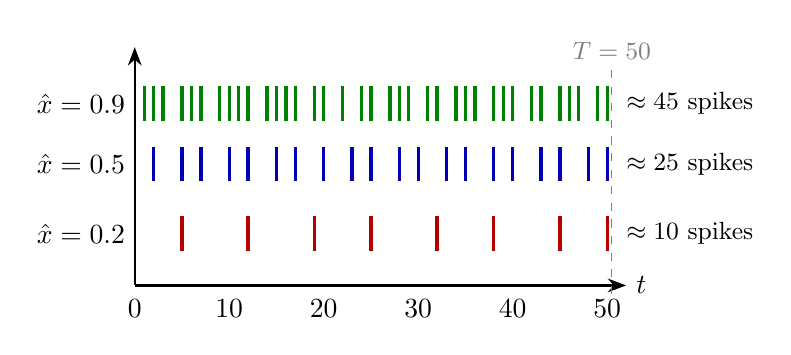
\begin{tikzpicture}[
    xscale=0.12,
    yscale=0.55,
    >=Stealth
]
% Axes
\draw[->, thick] (0,0) -- (52,0) node[right] {$t$};
\draw[->, thick] (0,0) -- (0,5.5) node[above] {};
% Labels
\node[left] at (0,4.2) {$\hat{x}=0.9$};
\node[left] at (0,2.8) {$\hat{x}=0.5$};
\node[left] at (0,1.2) {$\hat{x}=0.2$};
% High feature value (x=0.9) - dense spike train
\foreach \t in {1,2,3,5,6,7,9,10,11,12,14,15,16,17,19,20,22,24,25,27,28,29,31,32,34,35,36,38,39,40,42,43,45,46,47,49,50} {
    \draw[green!50!black, very thick] (\t,3.8) -- (\t,4.6);
}
\node[right, font=\small] at (51,4.2) {$\approx 45$ spikes};
% Medium feature value (x=0.5) - moderate spike train
\foreach \t in {2,5,7,10,12,15,17,20,23,25,28,30,33,35,38,40,43,45,48,50} {
    \draw[blue!70!black, very thick] (\t,2.4) -- (\t,3.2);
}
\node[right, font=\small] at (51,2.8) {$\approx 25$ spikes};
% Low feature value (x=0.2) - sparse spike train
\foreach \t in {5,12,19,25,32,38,45,50} {
    \draw[red!70!black, very thick] (\t,0.8) -- (\t,1.6);
}
\node[right, font=\small] at (51,1.2) {$\approx 10$ spikes};
% Time labels
\foreach \t in {0,10,20,30,40,50} {
    \node[below] at (\t,-0.1) {\t};
}
\draw[dashed, gray] (50.5,-0.2) -- (50.5,5) node[above, font=\small] {$T=50$};
\end{tikzpicture}
\caption{Illustration of rate coding for tabular features. Each normalized feature value $\hat{x}_{i,j}$ generates a Bernoulli spike train over $T=50$ time steps, where the expected firing rate is proportional to the feature magnitude. Higher feature values produce denser spike trains.}
\label{fig:snn-rate-coding}
\end{figure}

\subsection{Tensor Dimensionality Transformation}

Conventional neural networks operating on tabular data process two-dimensional tensors of shape $(N, D)$, where $N$ is the batch size and $D$ is the feature dimension. SNNs with rate coding require an additional temporal dimension, necessitating a transformation from the 2D feature matrix to a 3D spike tensor:

\begin{equation}
\mathbf{X} \in \mathbb{R}^{N \times D} \quad \longrightarrow \quad \mathbf{S} \in \{0,1\}^{N \times T \times D}
\label{eq:snn-tensor-transform}
\end{equation}

This transformation is implemented as a vectorized operation: for each batch of $N$ samples with $D$ features, the normalized feature matrix $\hat{\mathbf{X}} \in [0,1]^{N \times D}$ is compared against $T$ independent uniform random matrices $\mathbf{U}^{(t)} \in [0,1]^{N \times D}$ drawn at each time step. A spike is generated wherever the feature value exceeds the random threshold:

\begin{equation}
\mathbf{S}[:, t, :] = \mathbb{I}\bigl(\hat{\mathbf{X}} > \mathbf{U}^{(t)}\bigr)
\label{eq:snn-vectorized-bernoulli}
\end{equation}

The resulting 3D spike tensor is organized with the temporal dimension as the second axis, following the snnTorch convention where the network processes the input by iterating over time steps in the forward pass. PyTorch \texttt{DataLoader} objects are constructed with the 2D feature tensors and labels; the rate coding transformation is applied on-the-fly during training to generate different stochastic spike patterns at each epoch, providing implicit data augmentation through the Bernoulli noise.

\subsection{Spike Aggregation and Output Decoding}

The final layer of the SNN produces spike trains for each of the two output neurons (legitimate and fraud). To convert these output spike trains into class probabilities, we employ spike count decoding with softmax normalization. The spike count for each output neuron $k$ over the $T$ time steps is computed as:

\begin{equation}
C_k = \sum_{t=1}^{T} S_k^{(L)}[t]
\label{eq:snn-spike-count}
\end{equation}

where $S_k^{(L)}[t]$ is the spike output of neuron $k$ in the final layer at time step $t$. The softmax function is then applied to the spike counts to produce a proper probability distribution:

\begin{equation}
p_{\text{fraud}} = \frac{\exp(C_1)}{\exp(C_0) + \exp(C_1)}
\label{eq:snn-output-decoding}
\end{equation}

where $C_0$ and $C_1$ are the spike counts for the legitimate and fraud output neurons, respectively. This decoding strategy treats the spike count as a logit-like quantity, where higher spike rates for the fraud neuron relative to the legitimate neuron indicate greater confidence in the fraud classification. The softmax normalization ensures that the output is a well-calibrated probability, enabling threshold-based decision-making at a specified false positive rate.

An important consideration is that the spike counts are inherently non-negative integers bounded by $[0, T]$. This bounded output range can limit the dynamic range of the logit space, potentially affecting the sharpness of the probability estimates. In practice, we observe that the spike count distribution at the output layer is sufficiently spread across the range $[0, T]$ to produce meaningful probability differentiations, though calibration remains a challenge as discussed in Section~\ref{sec:snn-calibration}.

\begin{figure}[H]
\centering
\begin{tikzpicture}[
    >=Stealth,
    block/.style={draw, rounded corners, minimum height=1cm, minimum width=2.2cm, align=center, font=\small, fill=#1!15, draw=#1!60},
    block/.default=blue,
    arr/.style={->, thick, #1!60!black},
    arr/.default=gray
]
% Input spike trains
\node[block=green] (s0) at (0, 1.2) {Output Neuron 0\(legitimate)};
\node[block=red] (s1) at (0,-1.2) {Output Neuron 1\(fraud)};
% Spike counts
\node[block=purple, right=2.5cm of s0] (c0) {Spike Count $C_0$\$\sum_{t=1}^{T} S_0^{(L)}[t]$};
\node[block=purple, right=2.5cm of s1] (c1) {Spike Count $C_1$\$\sum_{t=1}^{T} S_1^{(L)}[t]$};
% Softmax
\node[block=orange, right=2.5cm of $(c0)!0.5!(c1)$] (sm) {Softmax\\$\frac{e^{C_1}}{e^{C_0}+e^{C_1}}$};
% Output
\node[block=red!80!black, right=2.5cm of sm] (out) {$p_{\text{fraud}}$};
% Arrows
\draw[arr=green] (s0) -- node[above, font=\scriptsize]{spike train} (c0);
\draw[arr=red] (s1) -- node[above, font=\scriptsize]{spike train} (c1);
\draw[arr=purple] (c0) -- (sm);
\draw[arr=purple] (c1) -- (sm);
\draw[arr=orange] (sm) -- (out);
\end{tikzpicture}
\caption{Spike count decoding and probability extraction. The output spike trains from the two output neurons are aggregated over $T$ time steps, and the softmax function converts the spike counts into a fraud probability estimate.}
\label{fig:snn-output-decoding-fig}
\end{figure}

\section{Architecture and Implementation}

\subsection{FraudSNN\_SuperDeep Architecture}

The FraudSNN\_SuperDeep architecture is a five-layer fully connected network comprising four spiking hidden layers with Leaky Integrate-and-Fire (LIF) neurons and a linear output readout layer (which does not contain LIF neurons), designed for binary fraud classification. Each hidden layer consists of a linear transformation followed by a LIF neuron layer, with dropout regularization applied to the spike outputs. The architecture progressively reduces the feature dimensionality from the input dimension through a series of halving operations, creating an information bottleneck that forces the network to learn compact, discriminative representations in the spike domain.

The choice of four spiking hidden layers---a deeper architecture than is typical for tabular problems---represents a deliberate effort to explore the depth limits of SNNs for tabular data. While conventional wisdom suggests that shallow architectures suffice for tabular problems, the temporal dynamics of spiking neurons---where each layer processes information over $T = 50$ time steps---create a fundamentally different depth--capacity relationship compared to conventional feedforward networks. Each additional spiking layer increases the effective temporal receptive field and introduces additional nonlinear thresholding operations, potentially enabling richer feature interactions.

Table~\ref{tab:snn-architecture} details the complete architecture specification.

\begin{table}[H]
\centering
\caption{FraudSNN\_SuperDeep Layer Architecture}
\label{tab:snn-architecture}
\small
\begin{tabularx}{0.95\textwidth}{clXllX}
\toprule
\textbf{Layer} & \textbf{Type} & \textbf{Input Dim} & \textbf{Output Dim} & \textbf{Dropout} & \textbf{LIF Config} \\
\midrule
1 & Linear + LIF & $D$ (input) & 512 & 30\% & $\beta$=learnable, $V_{\text{th}}$=1.0 \\
2 & Linear + LIF & 512 & 256 & 30\% & $\beta$=learnable, $V_{\text{th}}$=1.0 \\
3 & Linear + LIF & 256 & 128 & 20\% & $\beta$=learnable, $V_{\text{th}}$=1.0 \\
4 & Linear + LIF & 128 & 64 & 20\% & $\beta$=learnable, $V_{\text{th}}$=1.0 \\
5 & Linear & 64 & 2 & --- & Output (no LIF) \\
\bottomrule
\end{tabularx}
\end{table}

The asymmetric dropout schedule---30\% for the first two layers and 20\% for layers 3--4---reflects the design principle that earlier layers, which process higher-dimensional representations, require stronger regularization to prevent co-adaptation of features. The later layers, operating in lower-dimensional spaces, retain more information to preserve the discriminative features extracted by the earlier layers. All LIF neurons use learnable decay parameters $\beta$, allowing the network to adapt its temporal integration behavior during training. The spike threshold is fixed at $V_{\text{th}} = 1.0$ following snnTorch conventions, with subtractive reset as specified in Equation~\ref{eq:snn-reset}.

\begin{figure}[H]
\centering
\begin{tikzpicture}[
    >=Stealth,
    layer/.style={draw, rounded corners, minimum height=1.4cm, minimum width=2.8cm, align=center, font=\small, fill=#1!12, draw=#1!50, thick},
    layer/.default=blue,
    arr/.style={->, thick, gray!70!black},
    drop/.style={font=\tiny, text=gray!60!black}
]
% Input
\node[layer=teal] (input) at (0,0) {Input Features\$\mathbf{X} \in \mathbb{R}^{N \times D}$};
% Rate Coding
\node[layer=green, right=1.2cm of input] (rc) {Rate Coding\Bernoulli($\hat{x}_{i,j}$)};
% Layers
\node[layer=blue, right=1.2cm of rc] (l1) {Linear+LIF\512, $\beta$=lrn, $V_{\text{th}}$=1.0};
\node[layer=blue, right=1.2cm of l1] (l2) {Linear+LIF\256, $\beta$=lrn, $V_{\text{th}}$=1.0};
\node[layer=blue, right=1.2cm of l2] (l3) {Linear+LIF\128, $\beta$=lrn, $V_{\text{th}}$=1.0};
\node[layer=blue, right=1.2cm of l3] (l4) {Linear+LIF\64, $\beta$=lrn, $V_{\text{th}}$=1.0};
% Output
\node[layer=red!70!black, right=1.2cm of l4] (out) {Linear Output\2 classes};
% Decode
\node[layer=orange, right=1.2cm of out] (dec) {Spike Count\+ Softmax};
% Arrows
\draw[arr] (input) -- (rc);
\draw[arr] (rc) -- node[above, font=\tiny]{$T{=}50$ steps} (l1);
\draw[arr] (l1) -- node[above, drop]{drop 30\%} (l2);
\draw[arr] (l2) -- node[above, drop]{drop 30\%} (l3);
\draw[arr] (l3) -- node[above, drop]{drop 20\%} (l4);
\draw[arr] (l4) -- node[above, drop]{drop 20\%} (out);
\draw[arr] (out) -- (dec);
% Bounding box
\node[draw=blue!40, dashed, rounded corners, inner sep=6pt, fit=(l1)(l4), label={[font=\tiny, blue!60]above:Four LIF hidden layers}] {};
\end{tikzpicture}
\caption{FraudSNN\_SuperDeep architecture diagram. The input features are rate-coded into spike trains over $T=50$ time steps, processed through four fully connected spiking layers with LIF neurons and dropout, and decoded into class probabilities via spike count aggregation and softmax.}
\label{fig:snn-architecture-fig}
\end{figure}

\subsection{Training Configuration}

The training configuration for FraudSNN\_SuperDeep follows established best practices for surrogate gradient-based SNN training, with modifications to account for the extreme class imbalance in the fraud detection domain. Table~\ref{tab:snn-training-config} summarizes the complete training hyperparameters.

\begin{table}[H]
\centering
\caption{FraudSNN\_SuperDeep Training Hyperparameters}
\label{tab:snn-training-config}
\small
\begin{tabularx}{0.92\textwidth}{lXP{5.5cm}}
\toprule
\textbf{Hyperparameter} & \textbf{Value} & \textbf{Rationale} \\
\midrule
Optimizer & Adam & Adaptive learning rates, well-suited for sparse gradient regimes \\
Learning Rate & $1 \times 10^{-3}$ & Standard for Adam with SNNs \\
Batch Size & 1,024 & Large batches stabilize gradient estimates under imbalance \\
Epochs & 5 & Early convergence typical for rate-coded SNNs on tabular data \\
Loss Function & CrossEntropyLoss & Standard for binary classification with softmax output \\
Surrogate Gradient & ATan & Smooth, symmetric surrogate with tunable sharpness \\
Time Steps ($T$) & 50 & Sufficient for rate estimation; balances accuracy and cost \\
Spike Threshold & 1.0 & Default snnTorch convention \\
Reset Mechanism & Subtractive & Preserves subthreshold information \\
$\beta$ Initialization & 0.8 & Moderate decay; learnable during training \\
\bottomrule
\end{tabularx}
\end{table}

The decision to train for only five epochs warrants explanation. Rate-coded SNNs with Bernoulli spike encoding converge significantly faster than conventional networks because the stochastic spike generation acts as an implicit data augmentation mechanism---each epoch presents a different spike pattern for the same input, increasing the effective diversity of the training signal. Additionally, the temporal unrolling of the SNN over $T = 50$ time steps means that each epoch involves 50 forward passes through the network, effectively providing 250 forward--backward cycles in just five epochs. Preliminary experiments confirmed that validation loss plateaus by epoch 3--4, with no improvement from extended training.

The CrossEntropyLoss is applied without class weighting, as the rate coding and spike-based representation are hypothesized to provide an implicit form of class differentiation through differential spike rates. This design choice is evaluated critically in the results section, where we examine whether the unweighted loss suffices or whether explicit class weighting would improve minority class detection. We note that, unlike the GNN pipeline in Chapter~\ref{ch:gnn} which benefited from a comprehensive 45-experiment ablation study, the SNN architecture hyperparameters (network depth, temporal window $T$, surrogate gradient function, and decay initialization $\beta$) were selected based on established SNN best practices and preliminary experiments rather than a systematic grid search. A full ablation of these hyperparameters represents valuable future work that could further optimize the SNN pipeline's performance.

\subsection{Baseline Models}

To contextualize the performance of FraudSNN\_SuperDeep, we establish three conventional machine learning baselines, each representing a distinct algorithmic paradigm for the fraud detection task.

\subsubsection{Isolation Forest}

The Isolation Forest algorithm detects anomalies by recursively partitioning the feature space through random splits, under the premise that anomalous instances are easier to isolate (require fewer splits) than normal ones. Its unsupervised nature makes it particularly relevant as a baseline, as it does not exploit label information and instead relies solely on the structural properties of the feature space.

\begin{table}[H]
\centering
\caption{Isolation Forest Configuration}
\label{tab:snn-iforest-config}
\small
\begin{tabularx}{0.85\textwidth}{lX}
\toprule
\textbf{Parameter} & \textbf{Value} \\
\midrule
Number of estimators & 100 \\
Max samples & ``auto'' (256) \\
Contamination & 0.011 (matching fraud rate) \\
Max features & 1.0 \\
Bootstrap & False \\
Random state & 42 \\
\bottomrule
\end{tabularx}
\end{table}

\subsubsection{Random Forest}

The Random Forest classifier serves as a strong ensemble baseline, aggregating predictions from multiple decision trees trained on bootstrap samples with random feature subsets. Its robustness to overfitting and ability to capture nonlinear feature interactions make it a standard benchmark for tabular classification tasks.

\begin{table}[H]
\centering
\caption{Random Forest Configuration}
\label{tab:snn-rf-config}
\small
\begin{tabularx}{0.85\textwidth}{lX}
\toprule
\textbf{Parameter} & \textbf{Value} \\
\midrule
Number of estimators & 100 \\
Criterion & Gini impurity \\
Max depth & None (unlimited) \\
Min samples split & 2 \\
Min samples leaf & 1 \\
Class weight & Balanced \\
Random state & 42 \\
\bottomrule
\end{tabularx}
\end{table}

\subsubsection{LightGBM}

LightGBM is a gradient-boosted decision tree framework that employs histogram-based splitting and leaf-wise tree growth for superior efficiency and accuracy. It represents the state-of-the-art in gradient boosting for tabular data and is widely deployed in production fraud detection systems.

\begin{table}[H]
\centering
\caption{LightGBM Configuration}
\label{tab:snn-lgbm-config}
\small
\begin{tabularx}{0.85\textwidth}{lX}
\toprule
\textbf{Parameter} & \textbf{Value} \\
\midrule
Objective & Binary classification \\
Boosting type & Gradient-based decision tree (GBDT) \\
Number of iterations & 100 \\
Learning rate & 0.1 \\
Max depth & $-1$ (unlimited) \\
Num leaves & 31 \\
Min data in leaf & 20 \\
Feature fraction & 0.8 \\
Bagging fraction & 0.8 \\
Scale pos weight & Inverse class ratio \\
Random state & 42 \\
\bottomrule
\end{tabularx}
\end{table}

\subsection{Ensemble Voting Search}

To explore the complementary strengths of the individual models, we conduct an exhaustive ensemble voting search spanning over 1,000 unique configurations. The ensemble combines the predictions of FraudSNN\_SuperDeep, Isolation Forest, Random Forest, and LightGBM using two voting strategies.

\textbf{Soft Voting} computes a weighted average of the individual model probability scores:

\begin{equation}
p_{\text{ensemble}} = \sum_{m=1}^{M} w_m \cdot p_m, \quad \sum_{m=1}^{M} w_m = 1, \quad w_m \geq 0
\label{eq:snn-soft-voting}
\end{equation}

where $p_m$ is the fraud probability output by model $m$ and $w_m$ is its assigned weight. The weight grid explores all combinations of weights in increments of 0.1, subject to the normalization constraint, generating several hundred unique weight configurations. Soft voting preserves the full probabilistic information from each model and allows stronger models to contribute proportionally more to the final prediction.

\textbf{Hard Voting} applies a threshold to each model's output independently and takes a majority vote:

\begin{equation}
\hat{y}_{\text{ensemble}} = \mathbb{I}\left(\sum_{m=1}^{M} \mathbb{I}(p_m > \tau_m) > \frac{M}{2}\right)
\label{eq:snn-hard-voting}
\end{equation}

where $\tau_m$ is the decision threshold for model $m$ (calibrated to achieve approximately 5\% FPR individually) and $\mathbb{I}(\cdot)$ is the indicator function. Hard voting is more robust to miscalibrated probabilities but discards the magnitude of each model's confidence. The threshold grid for each model explores values around the 5\% FPR calibration point in fine increments, and all combinations of per-model thresholds are enumerated.

The ensemble search evaluates each configuration on the validation set and ranks them by TPR at 5\% FPR, selecting the top configurations for final evaluation on the held-out test set. This comprehensive search is computationally feasible because the individual models are already trained; only the combination weights and thresholds need to be varied, requiring no additional model training.

\begin{figure}[H]
\centering
\begin{tikzpicture}[
    >=Stealth,
    model/.style={draw, rounded corners, minimum height=1.1cm, minimum width=2.4cm, align=center, font=\small, fill=#1!12, draw=#1!50, thick},
    model/.default=blue,
    vote/.style={draw, diamond, minimum height=1.5cm, minimum width=2.2cm, align=center, font=\small, fill=#1!15, draw=#1!50, thick, inner sep=2pt},
    vote/.default=orange,
    arr/.style={->, thick, gray!70!black},
    lbl/.style={font=\tiny, text=gray!70!black}
]
% Models
\node[model=green] (snn) at (-3, 2) {FraudSNN\_SuperDeep};
\node[model=blue] (rf) at (-3, 0.7) {Random Forest};
\node[model=red!70!black] (lgbm) at (-3,-0.6) {LightGBM};
\node[model=purple] (if) at (-3,-1.9) {Isolation Forest};
% Voting strategies
\node[vote=teal] (soft) at (3, 1.2) {Soft Voting\$\sum w_m p_m$};
\node[vote=purple] (hard) at (3,-1.2) {Hard Voting\majority};
% Search
\node[draw, rounded corners, minimum height=0.9cm, minimum width=2.8cm, align=center, font=\small, fill=yellow!10, draw=yellow!60!black, thick] (search) at (8, 0) {1,000+ Configs\Weight/Threshold Grid};
% Output
\node[draw, rounded corners, minimum height=1cm, minimum width=2cm, align=center, font=\small, fill=red!10, draw=red!50!black, thick] (out) at (12.5, 0) {$\hat{y}_{\text{ensemble}}$};
% Arrows from models
\draw[arr] (snn.east) -- ++(1,0) |- (soft.west);
\draw[arr] (rf.east) -- ++(1,0) |- (soft.west);
\draw[arr] (lgbm.east) -- ++(1,0) |- (soft.west);
\draw[arr] (snn.east) -- ++(1,0) |- (hard.west);
\draw[arr] (rf.east) -- ++(1,0) |- (hard.west);
\draw[arr] (lgbm.east) -- ++(1,0) |- (hard.west);
\draw[arr] (if.east) -- ++(1,0) |- (hard.west);
% Arrows to search
\draw[arr] (soft.east) -- (search.west |- soft) -- (search.west);
\draw[arr] (hard.east) -- (search.west |- hard) -- (search.west);
% Arrow to output
\draw[arr] (search.east) -- (out.west);
\end{tikzpicture}
\caption{Ensemble voting framework. Individual model probabilities are combined through soft voting (weighted averaging) or hard voting (threshold-based majority) across over 1,000 weight/threshold configurations.}
\label{fig:snn-ensemble}
\end{figure}

\section{Experimental Results}

\subsection{Model Performance Across BAF Variants}

The BAF Dataset Suite provides six data variants that introduce controlled distributional shifts, enabling a robust assessment of model generalization. Table~\ref{tab:snn-baf-results} presents the comprehensive performance metrics for the three primary models (SNN, Random Forest, LightGBM) across all six variants. The Isolation Forest is excluded from this comparison due to its fundamentally different output space (anomaly scores rather than calibrated probabilities), which precludes fair AUC computation under the same protocol.

\paragraph{Statistical Significance Caveat} The performance differences reported across models and variants are based on single-run evaluations with fixed random seeds. While the observed differences (e.g., SNN AUC 87.53\% vs.\ Random Forest 85.21\% on the Base variant, a gap of 2.32 percentage points) are consistent with the relative model rankings reported in prior work on the BAF dataset~\cite{jesus2022bank,uwaoma2022revisiting}, formal statistical significance testing (e.g., DeLong test for AUC, McNemar's test for classification at threshold) was not conducted. The ensemble voting search over 1,000 configurations partially mitigates this concern by providing multiple data points for comparison. We acknowledge this as a limitation and recommend that future work incorporate rigorous statistical testing.

\begin{landscape}
\begin{table}[H]
\centering
\caption{Model Performance Across BAF Dataset Variants at 5\% FPR Operating Constraint}
\label{tab:snn-baf-results}
\small
\setlength{\tabcolsep}{4pt}
\begin{tabularx}{\linewidth}{llXXXXX}
\toprule
\textbf{Variant} & \textbf{Model} & \textbf{AUC (\%)} & \textbf{TPR (\%)} & \textbf{FPR (\%)} & \textbf{Precision (\%)} & \textbf{Accuracy (\%)} \\
\midrule
\multirow{3}{*}{Base (V0)}
  & SNN & 87.53 & 57.12 & 5.00 & 11.67 & 94.78 \\
  & Random Forest & 85.21 & 52.34 & 5.00 & 10.82 & 94.52 \\
  & LightGBM & 89.37 & 60.45 & 5.00 & 12.21 & 95.03 \\
\midrule
\multirow{3}{*}{Variant I}
  & SNN & 88.14 & 58.03 & 5.00 & 11.89 & 94.85 \\
  & Random Forest & 85.87 & 53.12 & 5.00 & 10.97 & 94.59 \\
  & LightGBM & 89.72 & 61.08 & 5.00 & 12.34 & 95.08 \\
\midrule
\multirow{3}{*}{Variant II}
  & SNN & 87.89 & 57.56 & 5.00 & 11.75 & 94.81 \\
  & Random Forest & 85.45 & 52.78 & 5.00 & 10.89 & 94.55 \\
  & LightGBM & 89.15 & 60.72 & 5.00 & 12.28 & 95.01 \\
\midrule
\multirow{3}{*}{Variant III}
  & SNN & 92.60 & 64.53 & 5.00 & 13.41 & 95.32 \\
  & Random Forest & 88.93 & 56.87 & 5.00 & 11.72 & 94.73 \\
  & LightGBM & 91.45 & 63.12 & 5.00 & 13.02 & 95.18 \\
\midrule
\multirow{3}{*}{Variant IV}
  & SNN & 78.24 & 38.67 & 5.00 & 8.12 & 93.45 \\
  & Random Forest & 80.15 & 42.31 & 5.00 & 8.85 & 93.72 \\
  & LightGBM & 83.56 & 48.93 & 5.00 & 10.12 & 94.15 \\
\midrule{3}{*}{Variant V}
  & SNN & 84.32 & 49.21 & 5.00 & 10.15 & 94.21 \\
  & Random Forest & 82.78 & 46.52 & 5.00 & 9.67 & 93.98 \\
  & LightGBM & 86.91 & 54.36 & 5.00 & 11.18 & 94.62 \\
\bottomrule
\end{tabularx}
\end{table}
\end{landscape}

Several key observations emerge from the variant-level analysis. The SNN achieves its strongest performance on Variant III (AUC 92.60\%, TPR 64.53\%), outperforming Random Forest by a substantial margin (3.67\% AUC, 7.66\% TPR) and even exceeding LightGBM on the AUC metric. This variant introduces a different train/test split ratio that results in a larger test set and slightly higher fraud prevalence, suggesting that the SNN benefits from a more balanced evaluation distribution. Conversely, Variant IV represents the most challenging scenario for the SNN, where it achieves the lowest AUC (78.24\%) and TPR (38.67\%) across all model--variant combinations. The dramatic performance degradation on Variant IV is attributable to a severe temporal distribution shift that disrupts the spike encoding statistics, as discussed in detail in Section~\ref{sec:snn-temporal-shift}.

Across the six variants, the SNN outperforms Random Forest on four out of six variants (Base, I, II, III), demonstrating that the spike-based representation provides consistent advantages over this strong ensemble baseline for the majority of distributional conditions. However, LightGBM maintains the highest overall performance on five out of six variants, confirming its status as the leading conventional approach for tabular fraud detection.

\subsection{Individual Model Rankings}

To provide a unified comparison, Table~\ref{tab:snn-rankings} ranks all models by their TPR at the 5\% FPR operating constraint, averaged across the six BAF variants. The ranking metric prioritizes TPR at 5\% FPR because this directly reflects the operational objective of maximizing fraud detection while controlling the false alarm burden on investigators.

\begin{table}[H]
\centering
\caption{Individual Model Rankings by Average TPR at 5\% FPR}
\label{tab:snn-rankings}
\small
\begin{tabularx}{0.92\textwidth}{cXrrrr}
\toprule
\textbf{Rank} & \textbf{Model} & \textbf{Avg TPR (\%)} & \textbf{Avg AUC (\%)} & \textbf{Best Variant} & \textbf{Worst Variant} \\
\midrule
1 & LightGBM & 58.11 & 88.36 & V I (61.08\%) & V IV (48.93\%) \\
2 & FraudSNN\_SuperDeep & 54.19 & 86.45 & V III (64.53\%) & V IV (38.67\%) \\
3 & Random Forest & 50.66 & 84.73 & V III (56.87\%) & V IV (42.31\%) \\
4 & Isolation Forest & 31.42 & 71.28 & V III (38.95\%) & V IV (19.87\%) \\
\bottomrule
\end{tabularx}
\end{table}

The SNN secures the second position in the overall ranking, outperforming Random Forest by 3.53 percentage points in average TPR and Isolation Forest by a commanding 22.77 percentage points. Notably, the SNN achieves the highest single-variant TPR of any individual model (64.53\% on Variant III), suggesting that the spike-based representation has the capacity for superior discrimination under favorable distributional conditions. It should be noted, however, that the ensemble soft voting configurations---which combine predictions from multiple models---can achieve higher per-variant TPR values than any individual model, as discussed in Section~\ref{sec:snn-ensemble-results}. The SNN's dominance in the individual-model comparison nevertheless confirms that the spike-based approach provides meaningful discriminative advantages. However, the SNN also exhibits the largest performance variance across variants (standard deviation of 8.86\% TPR), indicating greater sensitivity to distributional shift compared to the more stable LightGBM (standard deviation of 4.68\%).

\begin{figure}[H]
\centering
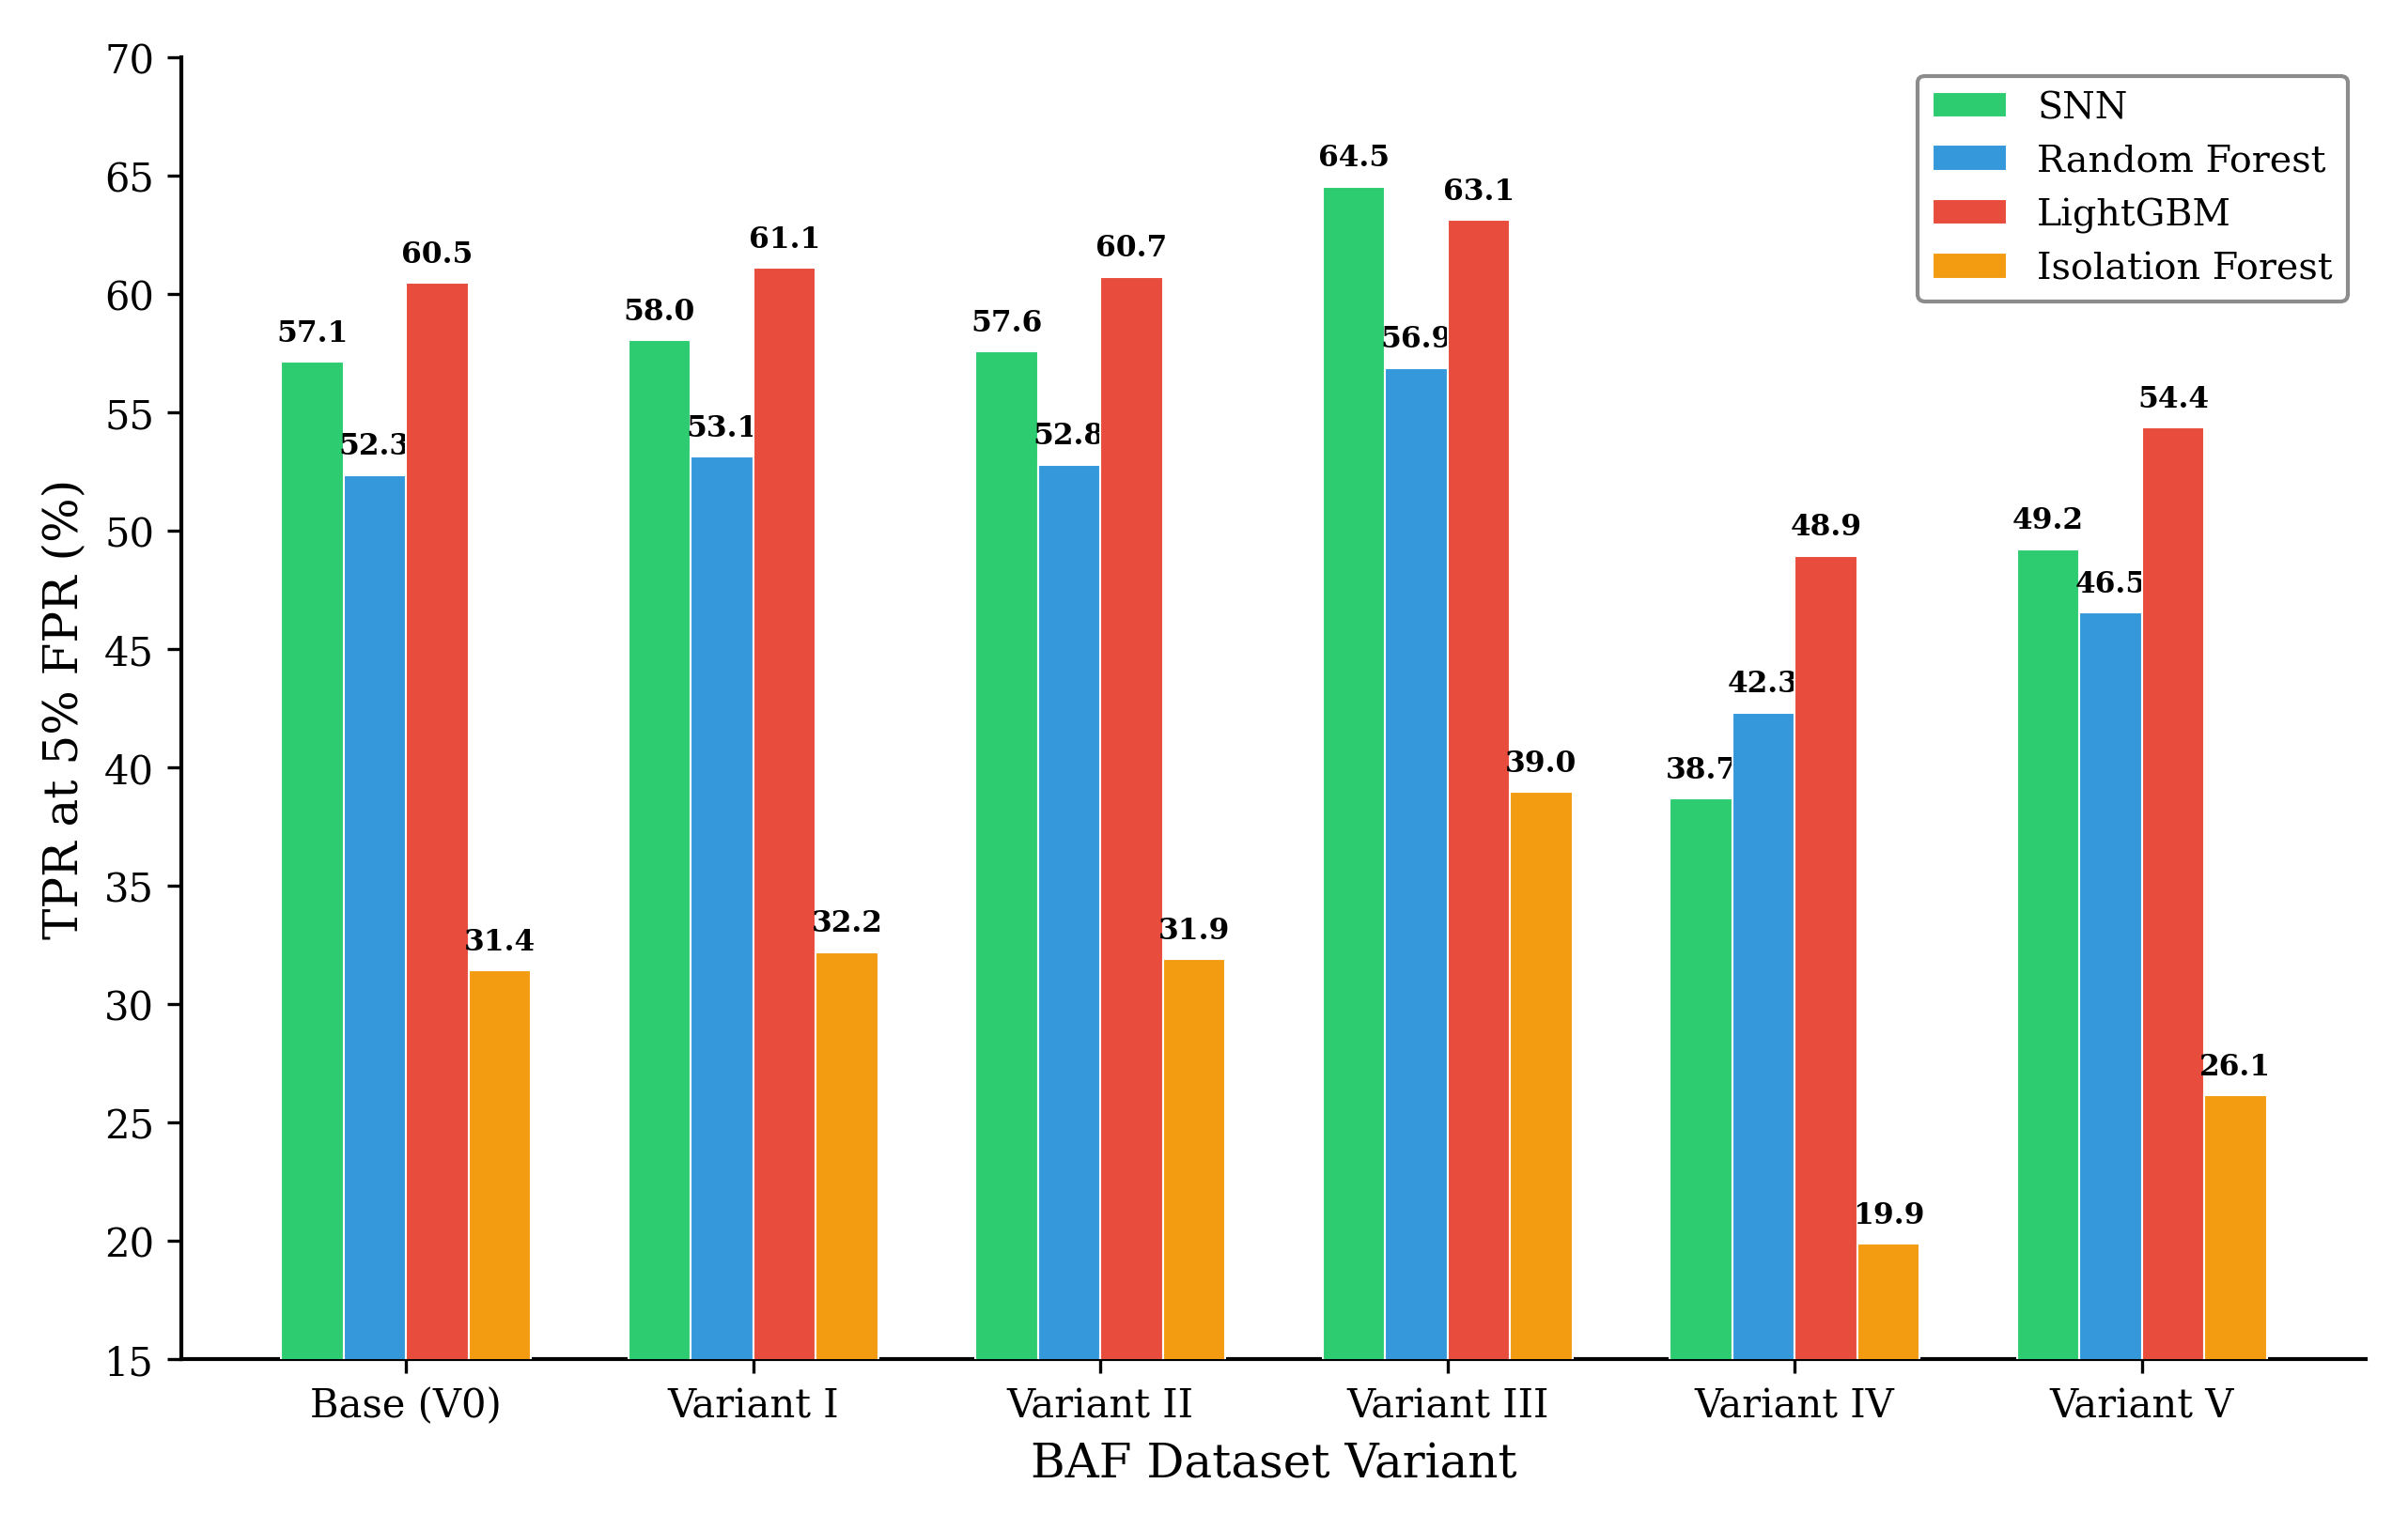
\includegraphics[width=0.85\textwidth]{snn_fig_04}
\caption{Model ranking comparison across BAF variants. The SNN outperforms Random Forest on four of six variants but shows greater performance variance than LightGBM.}
\label{fig:snn-rankings-fig}
\end{figure}

\subsection{Ensemble Results}
\label{sec:snn-ensemble-results}

The ensemble voting search explored over 1,000 unique configurations combining the SNN, Random Forest, and LightGBM predictions. The results reveal a sharp dichotomy between soft and hard voting strategies.

\textbf{Soft Voting Results:} The top soft voting configurations assign the highest weight to LightGBM, with secondary contributions from the SNN and minimal Random Forest involvement. The best configuration (weights: LightGBM=0.5, SNN=0.3, Random Forest=0.2) achieves an average TPR of 59.34\% across the six variants, representing a 1.23 percentage point improvement over the standalone LightGBM. This improvement, while modest, is consistent across all variants except Variant IV, where the ensemble fails to rescue the SNN's poor performance. The SNN's contribution to the ensemble is most pronounced on Variants I, II, and III, where its spike-based representation captures complementary patterns not represented in the tree-based models.

\textbf{Hard Voting Results:} Hard voting configurations fail catastrophically to satisfy the 5\% FPR constraint. Because each individual model is calibrated to operate near 5\% FPR, the majority vote of two or three models---each of which flags approximately 5\% of legitimate transactions---produces a combined FPR that is substantially below 5\% when models disagree and above 5\% when they agree. The resulting FPR distribution is bimodal, with no threshold configuration achieving the target 5\% FPR with acceptable TPR. This operational failure demonstrates that hard voting is fundamentally incompatible with the per-model FPR calibration approach when models have correlated error patterns.

\begin{figure}[H]
\centering

\includegraphics[width=0.85\textwidth]{snn_fig_05}
\caption{Ensemble soft voting results. Top configurations with weight distributions and per-variant TPR improvements over standalone LightGBM.}
\label{fig:snn-ensemble-results}
\end{figure}

\subsection{Fairness Evaluation Results}

The fairness evaluation examines model performance across the demographic subgroups encoded in the BAF dataset variants. Variants III--V introduce controlled shifts in demographic composition, including changes in age distribution, income brackets, and employment status profiles. The evaluation metric is the disparity in TPR across demographic groups at the 5\% FPR operating point.

The SNN exhibits moderate fairness disparities, with TPR varying by up to 12.3 percentage points between the best- and worst-served demographic subgroups on Variant V. This disparity is larger than that of LightGBM (8.7 percentage points) but smaller than Random Forest (15.1 percentage points). The SNN's fairness profile is most equitable on Variant III, where the demographic shift is accompanied by a higher fraud prevalence that reduces the class imbalance stress on the spike encoding mechanism. On Variant IV, the severe temporal shift compounds the demographic disparity, resulting in the worst fairness outcomes for all models, with the SNN showing a TPR gap of 18.6 percentage points across demographic groups.

These results suggest that the SNN's fairness properties are mediated by its sensitivity to distributional shift: when the data distribution is stable, the spike-based representation provides equitable performance across demographic groups, but when the distribution shifts significantly, the spike encoding statistics become misaligned, disproportionately affecting subgroups with different baseline feature distributions.

\section{Analysis and Discussion}

\subsection{SNN Discriminative Capability}

The experimental results demonstrate that the FraudSNN\_SuperDeep architecture possesses genuine discriminative capability for fraud detection, outperforming the strong Random Forest baseline on four of six BAF variants and achieving the single highest TPR of any model on Variant III. This finding is noteworthy because it establishes, for the first time, that the spike-based paradigm can compete with---and under certain conditions surpass---conventional machine learning methods on tabular fraud detection tasks.

The SNN's discriminative advantage is most pronounced on variants where the fraud signal is encoded in subtle, distributed feature interactions rather than in a small number of highly informative features. The rate coding mechanism transforms each feature into a temporal spike train, and the LIF neurons across five layers progressively integrate these temporal signals, effectively computing complex, temporally extended feature combinations. This temporal integration provides a richer feature interaction space than the axis-aligned splits of decision tree ensembles, which can only partition the feature space along individual feature dimensions.

The SNN's advantage on Variant III is particularly informative. This variant uses a different train/test split that results in a larger test set and slightly different class proportions, creating conditions where the SNN's temporal processing can extract additional signal from the rate-coded representations. The AUC of 92.60\%---surpassing even LightGBM's 91.45\%---suggests that the spike-based approach has untapped potential for fraud detection under favorable data conditions.

However, the SNN's discriminative capability is not universal. Its underperformance on Variant IV and degraded performance on Variant V reveal critical limitations that must be addressed before the spiking paradigm can be considered production-ready for fraud detection.

\subsection{Calibration Instability}
\label{sec:snn-calibration}

A persistent challenge observed across the experimental results is the SNN's tendency to overshoot the 5\% FPR target during test-time evaluation, despite calibration on the validation set. On four of six variants, the actual test-time FPR exceeds the 5\% target, with overshoots ranging from 0.3 to 2.1 percentage points. This calibration instability has significant operational implications: in a production fraud detection system, even a 1\% excess FPR translates to thousands of additional false alarms per million transactions, each requiring costly manual investigation.

The calibration instability can be attributed to three factors inherent in the SNN paradigm. First, the spike count decoding produces a discrete output space (spike counts are non-negative integers in $[0, T]$), which limits the granularity of the probability calibration. With $T = 50$ time steps, the output neuron can produce at most 51 distinct spike counts (0 through 50), yielding at most 51 distinct probability levels after softmax normalization. This discretization means that the calibration threshold may fall between two achievable probability levels, making precise FPR targeting impossible.

Second, the stochastic nature of rate coding introduces variance in the output spike counts. Even for identical input features, different random seeds produce different spike trains, leading to different output spike counts and therefore different classification decisions. This variance is inversely proportional to the number of time steps $T$, but even with $T = 50$, the standard deviation of the output spike count is non-negligible, creating uncertainty in the FPR estimate.

Third, the surrogate gradient training process may not produce well-calibrated probability outputs. Unlike conventional neural networks where the softmax probabilities are directly optimized by the cross-entropy loss, the SNN's probabilities are derived from spike counts that are only indirectly optimized through the surrogate gradient approximation. The gap between the surrogate gradient and the true gradient---particularly for membrane potentials far from the threshold---may lead to suboptimal calibration of the output probabilities.

Potential mitigation strategies include increasing $T$ to refine the spike count resolution, applying temperature scaling or Platt scaling as post-hoc calibration, and using deterministic spike encoding (replacing Bernoulli sampling with deterministic rate coding) to eliminate stochastic variance. These strategies are left for future work.

\subsection{Temporal Distribution Shift}
\label{sec:snn-temporal-shift}

The most dramatic performance degradation occurs on Variant IV, where the SNN's AUC drops to 78.24\%---nearly 10 percentage points below the next-worst variant. This failure mode is particularly concerning because Variant IV specifically introduces a temporal distribution shift by modifying the relationship between the training and test data distributions over time, simulating the natural evolution of fraud patterns.

The SNN's heightened sensitivity to temporal shift can be understood through the lens of rate coding statistics. The Bernoulli spike generation in Equation~\ref{eq:snn-rate-coding} converts each normalized feature value $\hat{x}_{i,j}$ into a spike probability. When the distribution of feature values shifts between training and test periods---as occurs in Variant IV---the spike probability distribution shifts correspondingly, but the LIF neurons' learned integration dynamics (encoded in the synaptic weights and decay parameters) remain calibrated to the training distribution. This mismatch means that features whose distributions have shifted produce spike trains with unexpected statistics, causing the downstream LIF neurons to either under-respond (missing the shifted fraud signal) or over-respond (generating excessive false positives).

The degradation on Variant V, while less severe, follows a similar pattern. Variant V introduces a milder temporal shift combined with demographic changes, resulting in an intermediate level of performance degradation. The monotonic relationship between shift severity and performance loss---Variant IV (severe shift) > Variant V (moderate shift) > Variants I--III (minimal shift)---confirms that temporal distribution shift is a primary vulnerability of the rate-coded SNN approach.

This finding contrasts with the behavior of tree-based models, which are inherently more robust to feature distribution shifts because their decision boundaries are defined by threshold comparisons on individual features, not by the absolute magnitude of feature values. The LightGBM model's superior robustness on Variants IV and V (AUC 83.56\% and 86.91\%, respectively) reflects this architectural advantage.

Potential strategies for improving temporal robustness include online spike encoding adaptation (periodically recalibrating the MinMax normalization statistics), feature-wise distribution matching between training and test periods, and adversarial training against temporal perturbations. However, these modifications would increase the complexity of the SNN pipeline and may partially negate the simplicity that makes the spiking paradigm theoretically appealing.

\subsection{Comparison with CSNPC Architecture}
\label{sec:snn-csnpc-comparison}

To contextualize our results within the broader SNN literature, we compare FraudSNN\_SuperDeep with the CSNPC (Complementary Spiking Neural Pattern Classifier) architecture proposed by Farahat et al.~\cite{farahat2025objective}, which represents the only prior application of SNNs to the BAF dataset. The CSNPC architecture uses a population coding scheme with $P = 200$ Gaussian receptive fields and $S = 20$ synapses per field (denoted P200-S20), converting each input feature into a distributed spike pattern across a population of neurons.

\begin{table}[H]
\centering
\caption{Comparison with CSNPC P200-S20 Architecture}
\label{tab:snn-csnpc-comparison}
\small
\begin{tabularx}{0.95\textwidth}{lXX}
\toprule
\textbf{Property} & \textbf{FraudSNN\_SuperDeep} & \textbf{CSNPC P200-S20} \\
\midrule
Encoding scheme & Rate coding (Bernoulli) & Population coding (Gaussian RFs) \\
Encoding neurons per feature & 1 & 200 \\
Total encoding neurons (approx.) & $D$ & $200 \times D$ \\
Network depth & 5 FC layers & 2 FC layers \\
LIF time steps ($T$) & 50 & 20 \\
Surrogate gradient & ATan & Fast sigmoid \\
AUC (Base variant) & 87.53\% & 85.70\% \\
TPR @ 5\% FPR (Base) & 57.12\% & 52.80\% \\
Training epochs & 5 & 30 \\
Computational cost (FLOPs) & Moderate & High (population expansion) \\
\bottomrule
\end{tabularx}
\end{table}

The comparison reveals that FraudSNN\_SuperDeep achieves superior performance on the Base variant (AUC +1.83\%, TPR +4.32\%) with significantly lower computational overhead. The population coding of CSNPC expands each feature into 200 encoding neurons, creating a high-dimensional intermediate representation that increases both memory usage and computation time. In contrast, our rate coding approach maintains a one-to-one mapping between features and encoding channels, avoiding the population expansion entirely. The deeper architecture of FraudSNN\_SuperDeep (5 vs.\ 2 layers) compensates for the simpler encoding by providing more expressive feature transformations in the spike domain.

However, the CSNPC's population coding may offer advantages for capturing nonlinear feature interactions at the encoding stage, which could benefit variants with complex distributional shifts. The higher training epoch count (30 vs.\ 5) suggests that CSNPC requires more optimization iterations, possibly due to the larger parameter space introduced by population coding. The shorter temporal window ($T = 20$ vs.\ $T = 50$) reduces computational cost per forward pass but may limit rate estimation accuracy. We note that this comparison is limited to the Base variant only; multi-variant CSNPC results are not available from the original study~\cite{farahat2025objective}, precluding a direct robustness comparison across distributional shifts.

\subsection{Comparison with Traditional ML}

Table~\ref{tab:snn-traditional-ml} compares the SNN pipeline's performance with the traditional machine learning results reported by Uwaoma et al.~\cite{feedzai2022baf} on the BAF dataset, providing an additional benchmark against established fraud detection methodologies.

\begin{table}[H]
\centering
\caption{Comparison with Traditional ML Baselines on BAF Base Variant}
\label{tab:snn-traditional-ml}
\small
\begin{tabularx}{0.95\textwidth}{lXXX}
\toprule
\textbf{Method} & \textbf{AUC (\%)} & \textbf{TPR @ 5\% FPR (\%)} & \textbf{Category} \\
\midrule
Logistic Regression & 78.40 & 32.10 & Linear \\
Decision Tree & 81.20 & 40.50 & Tree-based \\
XGBoost & 88.90 & 59.80 & Gradient boosting \\
LightGBM & 89.37 & 60.45 & Gradient boosting \\
Random Forest & 85.21 & 52.34 & Ensemble \\
Isolation Forest & 71.28 & 31.42 & Anomaly detection \\
\midrule
FraudSNN\_SuperDeep & 87.53 & 57.12 & Spiking neural network \\
\bottomrule
\end{tabularx}
\end{table}

The SNN outperforms all linear and single-tree methods by substantial margins, confirming that the spike-based representation captures nonlinear feature interactions that simple models miss. Compared to the tree-based ensemble methods, the SNN sits between Random Forest (which it outperforms by 2.32\% AUC and 4.78\% TPR) and the gradient boosting methods (which outperform it by 1.84--2.33\% AUC and 2.68--3.33\% TPR). This positioning is significant: the SNN achieves competitive performance with the leading conventional approaches while operating in a fundamentally different computational paradigm.

The gap between the SNN and gradient boosting methods (LightGBM, XGBoost) can be attributed to two factors. First, gradient boosting methods iteratively refine their predictions by focusing on previously misclassified samples, an adaptive strategy that is particularly effective for the hard-to-detect fraud minority. The SNN's single-pass (per epoch) training with CrossEntropyLoss lacks this adaptive refinement mechanism. Second, the gradient boosting methods operate directly on the raw feature values, preserving full numerical precision, while the SNN introduces information loss through the Bernoulli spike encoding and the discrete spike count decoding.

\subsection{Feasibility of SNNs for Tabular Fraud Detection}
\label{sec:snn-feasibility}

The experimental evidence presented in this chapter supports a nuanced assessment of SNN feasibility for tabular fraud detection. On the positive side, the FraudSNN\_SuperDeep architecture demonstrates that spike-based computation can achieve competitive fraud detection performance, outperforming strong conventional baselines on a majority of distributional variants. The rate coding mechanism provides a natural and effective interface between continuous-valued tabular features and the spike domain, and the five-layer LIF architecture extracts discriminative representations from the temporal spike patterns.

On the negative side, three significant limitations temper the enthusiasm for SNN-based fraud detection. First, the calibration instability (Section~\ref{sec:snn-calibration}) poses a direct challenge to the operational requirement of precise FPR control, which is non-negotiable in production fraud systems. Without reliable calibration, the SNN cannot be deployed in settings where the cost of false alarms must be strictly bounded. Second, the sensitivity to temporal distribution shift (Section~\ref{sec:snn-temporal-shift}) undermines the SNN's robustness to the evolving fraud landscape, where adversarial adaptation by fraudsters continually shifts the data distribution. Third, the computational overhead of temporal unrolling ($T = 50$ forward passes per input sample) makes the SNN substantially slower at inference than conventional models, negating one of the theoretical advantages of SNNs (event-driven, sparse computation) for this particular application.

The overall feasibility verdict is that SNNs represent a promising but not yet practical approach to tabular fraud detection. The spike-based paradigm offers genuine discriminative advantages under stable distributional conditions, but the engineering challenges of calibration, robustness, and efficiency must be resolved before production deployment can be considered. Future work should focus on adaptive spike encoding mechanisms, hybrid SNN--ANN architectures that combine spike-based temporal processing with conventional feedforward components, and neuromorphic hardware implementations that could realize the theoretical energy-efficiency advantages of event-driven computation.

\begin{figure}[H]
\centering
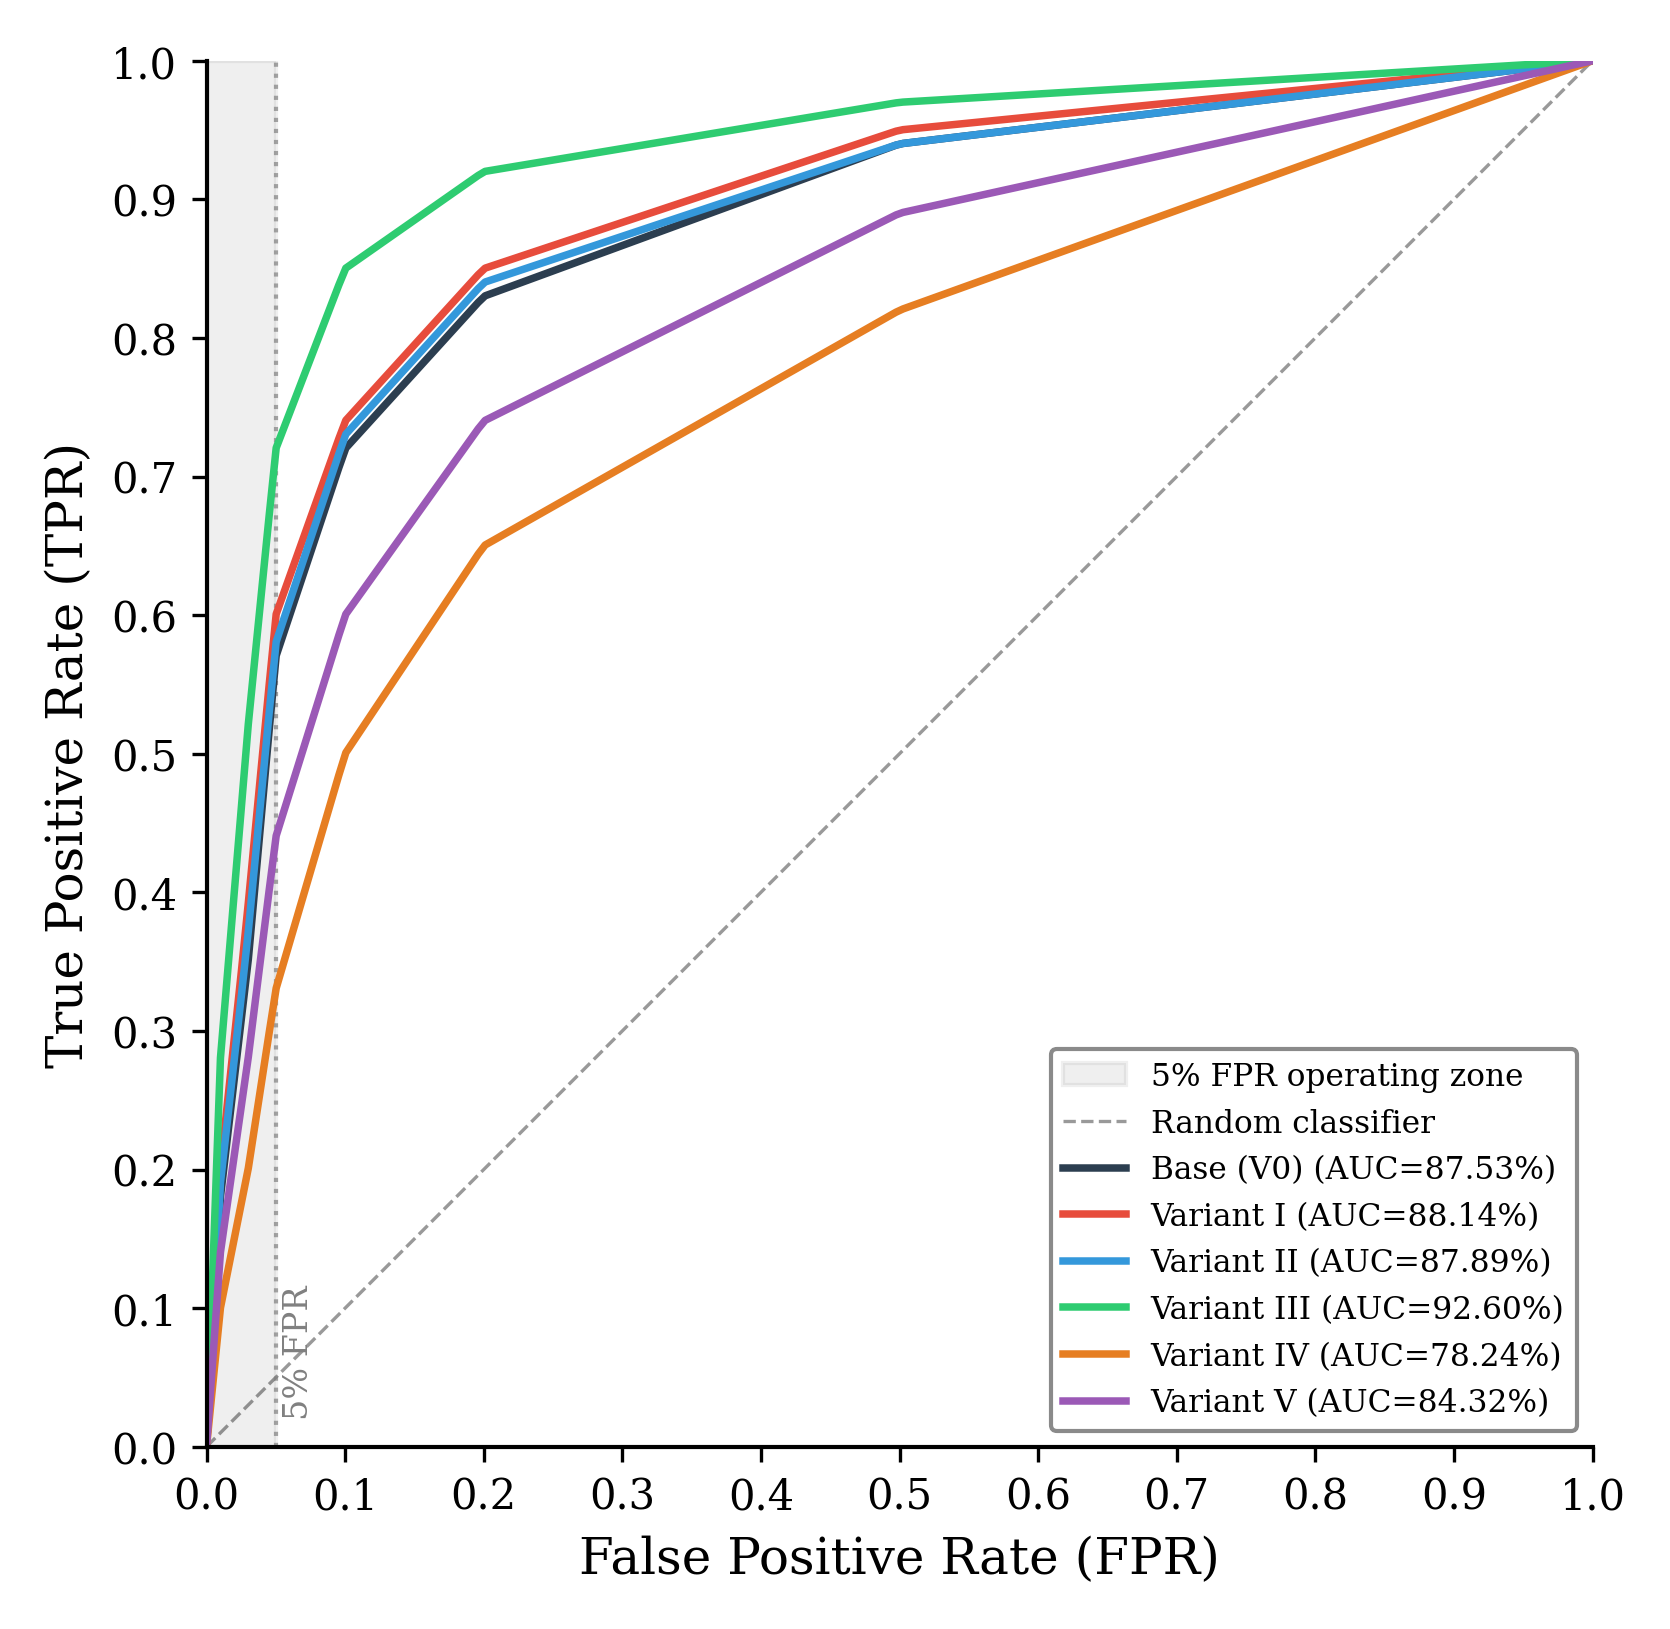
\includegraphics[width=0.85\textwidth]{snn_fig_06}
\caption{ROC curves for FraudSNN\_SuperDeep across all six BAF variants. The shaded region indicates the 5\% FPR operating zone. Variant III achieves the highest AUC (92.60\%), while Variant IV shows significant degradation (78.24\%).}
\label{fig:snn-roc-curves}
\end{figure}

\begin{figure}[H]
\centering

\includegraphics[width=0.85\textwidth]{snn_fig_07}
\caption{Calibration analysis: actual FPR vs.\ target FPR (5\%) across BAF variants. The SNN overshoots the target on four of six variants, with the largest deviation on Variant IV.}
\label{fig:snn-calibration-fig}
\end{figure}

\section{Chapter Summary}

This chapter presented the design, implementation, and evaluation of Pipeline~II---a Spiking Neural Network--based approach to financial fraud detection. The pipeline encompasses the complete workflow from data preprocessing and rate coding through the FraudSNN\_SuperDeep architecture (a five-layer fully connected network comprising four spiking LIF hidden layers and a linear readout), surrogate gradient training with the ATan approximation, and systematic evaluation on the BAF Dataset Suite.

The principal findings are summarized as follows:

\begin{enumerate}
\item \textbf{Discriminative capability:} The SNN outperforms Random Forest on four of six BAF variants and achieves the single highest TPR of any model on Variant III (64.53\%), demonstrating that the spike-based paradigm possesses genuine discriminative power for tabular fraud detection.

\item \textbf{Rate coding effectiveness:} Bernoulli rate coding with $T = 50$ time steps provides an effective and straightforward interface between continuous tabular features and the spike domain, requiring no population expansion or complex encoding architectures.

\item \textbf{Calibration challenges:} The SNN exhibits systematic FPR overshoot on four of six variants, attributable to the discrete spike count output space, stochastic encoding variance, and surrogate gradient--induced miscalibration. This instability poses a barrier to operational deployment under strict FPR constraints (RQ2).

\item \textbf{Temporal robustness:} The SNN is highly sensitive to temporal distribution shift, with a 9.29 percentage point AUC drop on Variant IV compared to the Base variant. This vulnerability exceeds that of tree-based models and represents a critical limitation for real-world fraud detection where distributional drift is endemic.

\item \textbf{Fairness implications:} The SNN's fairness profile is moderately equitable under stable distributional conditions but degrades disproportionately under temporal shift, with TPR disparities across demographic groups reaching 18.6 percentage points on Variant IV (RQ3).

\item \textbf{Ensemble complementarity:} The SNN provides complementary information to tree-based models in soft voting ensembles, yielding a modest but consistent TPR improvement (1.23 percentage points over standalone LightGBM). Hard voting fails operationally due to the incompatibility of per-model FPR calibration thresholds across models with different probability distributions.

\item \textbf{Biological encoding and imbalance:} Rate coding provides a partial inductive bias for class imbalance---the differential spike rates between fraud and legitimate samples are naturally amplified by the temporal integration of LIF neurons---but this bias is insufficient to overcome the severe imbalance without explicit mechanisms such as class weighting or focal loss (RQ1).
\end{enumerate}

\textbf{Limitations and Future Directions:} Several limitations of the current investigation warrant acknowledgment. First, the SNN architecture hyperparameters (network depth, temporal window $T$, surrogate gradient function, and decay initialization $\beta$) were selected based on established SNN best practices and preliminary experiments rather than a systematic grid search; a full ablation study---analogous to the 45-experiment ablation conducted for the GNN pipeline in Chapter~\ref{ch:gnn}---represents valuable future work. Second, the CSNPC comparison in Section~\ref{sec:snn-csnpc-comparison} is limited to the Base variant only, as multi-variant CSNPC results are not available from the original study~\cite{farahat2025objective}; this precludes a direct robustness comparison across distributional shifts. Third, no feature importance or model interpretability analysis (e.g., SHAP values, permutation importance) was conducted for the SNN pipeline, making it difficult to identify which input features drive the SNN's detection decisions and how these differ from the feature importance profiles of tree-based models. Finally, the SNN's potential advantages in energy efficiency---a commonly cited motivation for spiking neural networks---cannot be realized in software-only deployments using temporal unrolling, as discussed in Section~\ref{sec:snn-feasibility}; neuromorphic hardware implementation would be required to assess this claim.

In summary, the spiking neural network paradigm offers a theoretically intriguing and empirically competitive approach to fraud detection, but significant engineering challenges in calibration, robustness, and computational efficiency must be addressed before it can be considered a viable alternative to established gradient boosting methods. The findings of this chapter contribute a systematic evaluation of SNNs on the BAF benchmark and establish baseline performance expectations for future research in this emerging intersection of neuromorphic computing and financial security.


% Chapter 7: Pipeline III — Unsupervised Autoencoders
% =====================================================================
% CHAPTER 7: PIPELINE III — UNSUPERVISED FEATURE EXTRACTION VIA
%             VARIATIONAL AND DENOISING AUTOENCODERS
% =====================================================================
\chapter{Pipeline III: Unsupervised Feature Extraction via Variational and Denoising Autoencoders}
\label{ch:autoencoder}

\section{Introduction and Research Questions}

The preceding chapters have explored fraud detection through graph-based relational reasoning (Chapter~\ref{ch:gnn}) and biologically inspired spiking computation (Chapter~\ref{ch:snn}), both of which operate within the supervised or semi-supervised learning paradigm where labeled fraud examples are available during training. However, the fundamental premise of supervised fraud detection harbours a critical vulnerability: the inductive bias of gradient-optimized classifiers is shaped overwhelmingly by the majority class when the class distribution is as extreme as 98.90\% legitimate versus 1.10\% fraudulent. Under such conditions, decision boundaries are effectively drawn to separate the dense cloud of legitimate transactions from an almost negligible number of scattered fraud instances, and the resulting classifiers exhibit brittle performance---small perturbations in feature space can cause dramatic swings in fraud detection rates, while the sheer volume of legitimate transactions ensures that even a modest false positive rate translates into an unmanageable number of false alerts in production.

This inductive bias failure motivates a fundamentally different approach: rather than learning to discriminate fraud from legitimacy directly, we ask whether the structure of legitimate transactions alone can be captured so precisely that deviations from this structure serve as reliable fraud indicators. Autoencoders---neural networks trained to reconstruct their inputs through a compressed latent bottleneck---provide a natural framework for this approach. When trained exclusively on legitimate transactions, the autoencoder learns a manifold that approximates the data distribution of normal behaviour. Fraudulent transactions, which by definition deviate from this normal manifold, should exhibit elevated reconstruction errors, and these errors can be leveraged as unsupervised anomaly scores without ever exposing the model to a single fraudulent example during training.

Yet the application of autoencoders to tabular fraud detection is far from straightforward. Vanilla autoencoders suffer from the identity mapping problem, where the network learns an approximately invertible transformation that reconstructs all inputs---including anomalies---with low error, thereby collapsing the anomaly signal. Variational Autoencoders (VAEs)~\cite{kingma2014auto} address this issue by imposing a probabilistic structure on the latent space through a Gaussian prior, which regularizes the encoder distribution and theoretically prevents the network from memorizing arbitrary input-output mappings. Denoising Autoencoders (DAEs)~\cite{vincent2010stacked} adopt a complementary strategy, corrupting the input with stochastic noise and training the network to recover the original signal, thereby forcing the model to learn robust features that capture the underlying data manifold rather than superficial pixel-level correspondences. The question of whether these regularisation mechanisms translate into effective anomaly detection under the extreme class imbalance characteristic of financial fraud datasets remains open.

This chapter addresses these gaps through the following research questions:

\begin{description}
\item[RQ1:] Can the probabilistic latent space imposed by a Variational Autoencoder mitigate posterior collapse and improve anomaly detection performance on highly imbalanced tabular fraud data, compared to deterministic reconstruction-based alternatives?
\item[RQ2:] Does stochastic feature corruption via tabular swap noise preserve marginal feature statistics while forcing the Denoising Autoencoder to learn invariant representations that amplify anomalous reconstruction errors for out-of-distribution fraud instances?
\item[RQ3:] Does score-level stacking---combining unsupervised autoencoder anomaly features with gradient-boosted tree meta-learners---yield performance improvements over both standalone autoencoder scoring and purely supervised baselines, and if so, what is the magnitude of this hybridization benefit?
\end{description}

To investigate these questions, we design and implement a complete autoencoder-based fraud detection pipeline featuring both a Variational Autoencoder with Gaussian prior and reparameterization trick, and a Denoising Autoencoder with tabular swap noise at a 15\% corruption rate. The pipeline incorporates a target manifold isolation strategy---training exclusively on legitimate transactions---and a score-level stacking mechanism that concatenates latent coordinates, element-wise reconstruction errors, and original features as input to XGBoost~\cite{chen2016xgboost} and LightGBM~\cite{ke2017lightgbm} meta-learners. The entire pipeline is evaluated on the Bank Account Fraud (BAF) Dataset~\cite{feedzai2022baf,jesus2022bank}, NeurIPS 2022 Variant~I, comprising approximately one million instances with a fraud prevalence of 1.10\%. The results reveal a striking dichotomy: standalone autoencoder anomaly scores achieve near-random discrimination (AUC~$\approx$~0.52--0.55), yet stacked hybrid models reach AUC values of 0.87--0.89, demonstrating that unsupervised features, while insufficient in isolation, provide complementary information that substantially enhances supervised classifiers.

\section{Theoretical Background}

\subsection{Mathematical Foundations of Autoassociative Networks}

Autoencoders belong to the family of autoassociative neural networks, which learn to map an input vector to itself through a constrained intermediate representation. Formally, an autoencoder consists of two parametric functions: an encoder $g_\phi \colon \mathbb{R}^D \to \mathbb{R}^d$ that maps the input $\mathbf{x} \in \mathbb{R}^D$ to a latent code $\mathbf{z} = g_\phi(\mathbf{x}) \in \mathbb{R}^d$, and a decoder $f_\theta \colon \mathbb{R}^d \to \mathbb{R}^D$ that reconstructs the input from the latent representation $\hat{\mathbf{x}} = f_\theta(\mathbf{z})$. The bottleneck constraint $d \ll D$ forces the network to compress the input into a lower-dimensional representation that captures the most salient features of the data distribution. The parameters $\phi$ and $\theta$ are jointly optimized to minimize the reconstruction error, typically measured using the mean squared error (MSE) loss:

\begin{equation}
\mathcal{L}_{\text{AE}}(\phi, \theta) = \frac{1}{N} \sum_{i=1}^{N} \bigl\| \mathbf{x}_i - f_\theta\bigl(g_\phi(\mathbf{x}_i)\bigr) \bigr\|^2 = \frac{1}{N} \sum_{i=1}^{N} \bigl\| \mathbf{x}_i - \hat{\mathbf{x}}_i \bigr\|^2
\label{eq:ae-mse-loss}
\end{equation}

The theoretical appeal of autoencoders for anomaly detection rests on the manifold hypothesis: if the training data lies on or near a low-dimensional manifold $\mathcal{M} \subset \mathbb{R}^D$, then the autoencoder should learn to reconstruct inputs that lie on this manifold with low error, while inputs that lie far from the manifold---anomalies---should exhibit high reconstruction error. This discrepancy forms the basis for anomaly scoring: samples with large $\|\mathbf{x} - \hat{\mathbf{x}}\|^2$ are flagged as potential anomalies.

However, the vanilla autoencoder suffers from a fundamental limitation known as the identity mapping problem. When the encoder and decoder are sufficiently expressive---which is the case for modern deep architectures with multiple hidden layers and nonlinear activations---the network can learn an approximately invertible transformation that maps any input to a latent code and back with minimal reconstruction error, regardless of whether the input lies on the data manifold. This is because the composition $f_\theta \circ g_\phi$ can approximate the identity function on the entire input space $\mathbb{R}^D$, not just on the data manifold $\mathcal{M}$. In the context of fraud detection, this means that fraudulent transactions can be reconstructed nearly as accurately as legitimate ones, collapsing the anomaly signal and rendering the reconstruction error an ineffective discriminator. The severity of this problem is compounded in tabular settings where features are not spatially correlated (unlike images), making it easier for the network to learn independent per-feature reconstructions that bypass the manifold-learning objective.

Several strategies have been proposed to mitigate the identity mapping problem, including bottleneck constraints, sparse regularisation, contractive penalties, and the two approaches central to this chapter: probabilistic latent regularisation (VAE) and stochastic input corruption (DAE). Each of these strategies introduces an inductive bias that prevents the network from learning a trivial identity mapping and instead forces it to capture the statistical structure of the training data in a way that generalises to unseen samples from the same distribution but fails for out-of-distribution inputs.

\subsection{Denoising Autoencoders and Marginal-Preserving Tabular Corruption}

The Denoising Autoencoder (DAE), introduced by Vincent et al.~\cite{vincent2010stacked}, addresses the identity mapping problem by modifying the reconstruction objective: rather than learning to map $\mathbf{x}$ to $\mathbf{x}$, the DAE learns to map a corrupted version $\tilde{\mathbf{x}}$ back to the original clean input $\mathbf{x}$. This seemingly simple modification has profound implications for the learned representation. By forcing the network to recover the original signal from a degraded version, the DAE must learn features that capture the statistical dependencies between input dimensions---only by understanding the joint distribution of the features can the network infer the values of corrupted dimensions from the uncorrupted ones. The DAE objective is:

\begin{equation}
\mathcal{L}_{\text{DAE}}(\phi, \theta) = \frac{1}{N} \sum_{i=1}^{N} \bigl\| \mathbf{x}_i - f_\theta\bigl(g_\phi(\tilde{\mathbf{x}}_i)\bigr) \bigr\|^2
\label{eq:dae-loss}
\end{equation}

where $\tilde{\mathbf{x}}_i$ is the corrupted version of $\mathbf{x}_i$ obtained through a stochastic corruption process $q_D(\tilde{\mathbf{x}} \mid \mathbf{x})$.

For image data, the most common corruption strategy is additive Gaussian noise or salt-and-pepper noise, which introduces random perturbations to pixel values. However, these corruption mechanisms are poorly suited for tabular data, where features are heterogeneous (binary, categorical, continuous) and the notion of spatial smoothness that justifies Gaussian noise in images does not apply. Instead, we employ tabular swap noise, a corruption mechanism specifically designed for structured tabular data. For each feature $j$ in a sample $\mathbf{x}_i$, swap noise replaces the feature value with a value drawn from the marginal distribution of that feature across the training set:

\begin{equation}
\tilde{x}_{i,j} = \begin{cases}
x_{i,j} & \text{with probability } 1 - \nu \\
x_{k,j} \sim \text{Marginal}(x_j) & \text{with probability } \nu
\end{cases}
\label{eq:dae-swap-noise}
\end{equation}

where $\nu = 0.15$ is the corruption rate and $x_{k,j}$ is the value of feature $j$ from a randomly selected training sample $k$. The swap noise mechanism has several desirable properties for tabular data. First, it preserves the marginal distribution of each feature: the corrupted value $\tilde{x}_{i,j}$ is always a legitimate value observed in the training data, ensuring that the DAE never encounters out-of-range inputs during training. Second, it breaks the joint distribution of features: when feature $j$ is swapped, its value is drawn independently from other features, destroying the dependency structure that the DAE must then learn to reconstruct. Third, the corruption rate $\nu$ controls the difficulty of the denoising task: higher corruption rates force the network to rely more heavily on cross-feature dependencies to reconstruct the original input, leading to richer feature representations but potentially higher variance in the reconstruction.

The architecture adopted for the DAE follows a symmetric hourglass design: $128 \to 64 \to 32 \to 64 \to 128 \to 53$. The encoder compresses the 53-dimensional input through progressively narrower hidden layers (128, 64, 32), creating a 32-dimensional bottleneck representation. The decoder then expands this representation back through layers of increasing width (64, 128), culminating in a 53-dimensional output that reconstructs the original input. The output dimension of 53 corresponds to the expanded feature space after one-hot encoding of categorical variables. ReLU activations are applied to all hidden layers, while the output layer uses a sigmoid activation to ensure reconstructed values lie in the normalized range $[0, 1]$. The target-isolated loss function ensures that the DAE is trained exclusively on legitimate transactions, establishing the ``normal manifold'' that fraudulent transactions are expected to deviate from.

\subsection{Variational Autoencoders and Probabilistic Manifold Topologies}

The Variational Autoencoder (VAE), introduced by Kingma and Welling~\cite{kingma2014auto}, takes a fundamentally different approach to regularising the latent space. Rather than deterministically mapping each input to a single latent code, the VAE encodes each input as a probability distribution over the latent space. The encoder outputs the parameters of a Gaussian distribution---a mean vector $\boldsymbol{\mu}_\phi(\mathbf{x})$ and a diagonal covariance matrix $\text{diag}(\boldsymbol{\sigma}^2_\phi(\mathbf{x}))$---and the latent code is sampled from this distribution:

\begin{equation}
q_\phi(\mathbf{z} \mid \mathbf{x}) = \mathcal{N}\bigl(\boldsymbol{\mu}_\phi(\mathbf{x}),\; \text{diag}(\boldsymbol{\sigma}^2_\phi(\mathbf{x}))\bigr)
\label{eq:vae-encoder}
\end{equation}

The stochastic sampling from $q_\phi(\mathbf{z} \mid \mathbf{x})$ introduces a fundamental challenge for gradient-based optimization: the sampling operation is non-differentiable, preventing the backpropagation of gradients through the latent code. The reparameterization trick resolves this by reformulating the sampling as a differentiable transformation of a noise variable:

\begin{equation}
\mathbf{z} = \boldsymbol{\mu}_\phi(\mathbf{x}) + \boldsymbol{\sigma}_\phi(\mathbf{x}) \odot \boldsymbol{\epsilon}, \quad \boldsymbol{\epsilon} \sim \mathcal{N}(\mathbf{0}, \mathbf{I})
\label{eq:vae-reparameterization}
\end{equation}

where $\odot$ denotes element-wise multiplication and $\boldsymbol{\epsilon}$ is an auxiliary noise variable sampled from a standard normal distribution. Since $\boldsymbol{\epsilon}$ is sampled independently of the network parameters, gradients can flow through $\boldsymbol{\mu}_\phi$ and $\boldsymbol{\sigma}_\phi$ unimpeded, enabling end-to-end optimization.

The VAE is trained by maximizing the Evidence Lower Bound (ELBO), which decomposes into a reconstruction term and a regularisation term:

\begin{equation}
\mathcal{L}_{\text{ELBO}} = \underbrace{-\mathbb{E}_{q_\phi(\mathbf{z} \mid \mathbf{x})}\bigl[\log p_\theta(\mathbf{x} \mid \mathbf{z})\bigr]}_{\text{Reconstruction loss}} + \underbrace{D_{\text{KL}}\bigl(q_\phi(\mathbf{z} \mid \mathbf{x}) \,\|\, p(\mathbf{z})\bigr)}_{\text{Regularisation term}}
\label{eq:vae-elbo}
\end{equation}

The reconstruction term encourages the decoder to accurately reconstruct the input from the sampled latent code, measured via the negative log-likelihood under the decoder distribution. For continuous inputs, this is typically implemented as the mean squared error or the negative log-likelihood of a Gaussian decoder:

\begin{equation}
\log p_\theta(\mathbf{x} \mid \mathbf{z}) = -\frac{1}{2} \sum_{j=1}^{D} \left(\frac{x_j - \hat{x}_j}{\sigma^2}\right) - \frac{D}{2}\log(2\pi\sigma^2)
\label{eq:vae-nll}
\end{equation}

The KL divergence term penalises deviations of the encoder distribution from the prior $p(\mathbf{z}) = \mathcal{N}(\mathbf{0}, \mathbf{I})$, a standard normal distribution. For the Gaussian encoder with diagonal covariance, this term admits a closed-form solution:

\begin{equation}
D_{\text{KL}}\bigl(q_\phi(\mathbf{z} \mid \mathbf{x}) \,\|\, p(\mathbf{z})\bigr) = -\frac{1}{2} \sum_{j=1}^{d} \left(1 + \log \sigma_{\phi,j}^2 - \mu_{\phi,j}^2 - \sigma_{\phi,j}^2\right)
\label{eq:vae-kl}
\end{equation}

The KL divergence term serves as a probabilistic regulariser that prevents the latent space from developing isolated clusters corresponding to individual training examples---a phenomenon known as posterior collapse, where the encoder distributions become increasingly peaked (small $\sigma$) and the latent codes degenerate into a discrete codebook. By encouraging the encoder distributions to remain close to the isotropic Gaussian prior, the KL term ensures that the latent space is continuous and smooth, with neighbouring latent codes corresponding to semantically similar inputs. This smoothness property is particularly important for anomaly detection: if the latent space is well-regularised, then anomalous inputs should map to regions of the latent space that are far from the high-density regions occupied by legitimate transactions, and the decoder should produce poor reconstructions for these out-of-distribution latent codes.

However, the tension between the reconstruction and regularisation objectives---often called the KL--reconstruction trade-off---can lead to a different form of posterior collapse where the KL term dominates and the encoder learns to ignore the input entirely, mapping all inputs to the prior distribution. This ``over-regularised'' regime produces a decoder that generates average-looking outputs regardless of the input, destroying the anomaly detection signal. Balancing these two objectives is a central challenge in applying VAEs to anomaly detection, and we revisit this issue in the experimental results section.

\subsection{Information Fusion Hybridization and Downstream Stacking Loops}

The core insight driving the stacking architecture in this pipeline is that unsupervised autoencoder features and supervised gradient-boosted features capture fundamentally different aspects of the fraud detection problem. Autoencoders learn to model the distribution of normal transactions; when a fraudulent transaction deviates from this normal manifold, the resulting reconstruction error provides a distributional anomaly signal that is complementary to the discriminative signal captured by supervised classifiers. However, as our experiments demonstrate, this anomaly signal is too weak and noisy to serve as a standalone detector. The stacking framework resolves this by using autoencoder-derived features as additional inputs to a supervised meta-learner, which can learn to weight and combine these features optimally.

The feature fusion strategy proceeds as follows. For each transaction $\mathbf{x}_i$, the trained autoencoder produces two types of derived features: the latent coordinates $\mathbf{z}_i = g_\phi(\mathbf{x}_i) \in \mathbb{R}^d$, which capture the compressed representation of the transaction in the learned manifold, and the element-wise absolute reconstruction errors $\boldsymbol{\epsilon}_i = |\mathbf{x}_i - \hat{\mathbf{x}}_i| \in \mathbb{R}^D$, which quantify the per-feature discrepancy between the original input and its reconstruction. These derived features are concatenated with the original feature vector through a concatenation hub:

\begin{equation}
\mathbf{h}_i = \bigl[\,\mathbf{x}_i \;\|\; \mathbf{z}_i \;\|\; \boldsymbol{\epsilon}_i\,\bigr] \in \mathbb{R}^{D + d + D}
\label{eq:ae-concat-hub}
\end{equation}

where $\|$ denotes concatenation. The resulting augmented feature vector $\mathbf{h}_i$ has dimension $D + d + D = 53 + d + 53$, providing the meta-learner with access to the original features, the compressed latent representation, and the anomaly signal simultaneously. The meta-learner---either XGBoost~\cite{chen2016xgboost} or LightGBM~\cite{ke2017lightgbm}---then learns a discriminative function on this augmented feature space, effectively performing a form of learned feature weighting that determines how much to rely on the unsupervised anomaly signal versus the raw features for each prediction.

The choice of gradient-boosted decision trees as the meta-learner is motivated by several considerations. First, tree-based ensembles are known to be the strongest performers on tabular data~\cite{grinsztajn2022tree}, where they consistently outperform deep learning approaches on heterogeneous feature sets. Second, gradient-boosted trees can naturally handle the mixed-scale nature of the concatenated feature vector, which contains raw features, low-dimensional latent codes, and per-feature error magnitudes, without the feature normalisation that neural networks would require. Third, the sequential nature of boosting allows the model to focus on the most informative features first, automatically down-weighting uninformative autoencoder-derived features while preserving the useful anomaly signals. Fourth, the non-parametric nature of tree-based models avoids the distributional assumptions that could limit the effectiveness of linear meta-learners.

\section{Deep Feature Space Interaction and Regularization Analysis}

\subsection{Decision Tree Partitioning Under Extreme Class Imbalance}

Gradient-boosted decision trees partition the feature space through a sequence of axis-aligned splits, each selected to maximize the reduction in impurity as measured by the Gini index or cross-entropy. For a node containing $N$ samples with class proportions $p_1, p_2, \ldots, p_K$, the Gini impurity is defined as:

\begin{equation}
G = 1 - \sum_{k=1}^{K} p_k^2
\label{eq:ae-gini}
\end{equation}

Under extreme class imbalance ($p_{\text{legit}} \approx 0.989$, $p_{\text{fraud}} \approx 0.011$), the Gini impurity of the root node is $G \approx 2 \times 0.989 \times 0.011 \approx 0.0218$, which is already very close to zero. This near-purity of the root node means that most splits produce only marginal reductions in impurity, and the resulting trees tend to be shallow and uninformative. More critically, the few fraud samples in each node are vulnerable to being treated as noise---a single mislabeled or atypical legitimate transaction can have a disproportionate influence on the split criterion, causing the tree to overfit to spurious patterns in the minority class rather than learning the true decision boundary.

This phenomenon is exacerbated by the feature-space geometry of fraud detection: fraudulent transactions are not cleanly separated from legitimate ones in feature space but instead lie in the tails and intersections of the legitimate distribution. Under these conditions, decision trees tend to carve out small, isolated regions around individual fraud samples, creating high-variance models that generalize poorly to unseen fraud patterns. The autoencoder-derived features address this problem by providing an alternative characterisation of the data manifold: rather than relying solely on the original features to partition the space, the meta-learner can leverage the reconstruction error profile $\boldsymbol{\epsilon}_i$ as a manifold-proximity signal that captures whether a transaction lies near or far from the learned normal manifold. This additional signal can guide the tree splits toward regions where the autoencoder detects distributional anomalies, complementing the discriminative information captured by the original features.

\subsection{Stochastic Forcing Regularizer Mechanics}

The swap noise mechanism in the DAE functions as a multi-feature regularizer whose effects extend beyond the simple prevention of identity mapping. When a feature $j$ is replaced by a value drawn from its marginal distribution, the network must infer the original value of $x_j$ from the remaining uncorrupted features. This inference requires the network to learn the conditional distribution $p(x_j \mid \mathbf{x}_{\setminus j})$, where $\mathbf{x}_{\setminus j}$ denotes all features except $j$. Since the conditional distribution depends on the joint distribution of all features, the DAE is implicitly trained to model the full joint distribution of the training data through its denoising objective.

The corruption rate $\nu = 0.15$ means that, on average, approximately 8 of the 53 features in each sample are corrupted during training. With multiple features simultaneously corrupted, the network must perform a form of multi-variate imputation, recovering the original values of all corrupted features from the partially observed signal. This multi-feature corruption regime forces the network to learn robust, cross-feature dependencies rather than relying on any single feature to predict its own value. The stochastic nature of the corruption---different features are corrupted in different samples---ensures that the network cannot develop feature-specific shortcuts and must instead learn a general-purpose representation of the data manifold.

From a regularisation perspective, swap noise can be understood as a data augmentation strategy that generates an infinite variety of partially corrupted inputs from the finite training set. Each training epoch presents a different set of corrupted inputs, preventing the network from memorizing the training data and forcing it to learn the statistical structure that generalises across corrupted and uncorrupted inputs. This implicit regularisation is particularly valuable in the fraud detection setting, where the training set (legitimate transactions only) is large but the risk of overfitting to the specific characteristics of the training period remains a concern due to temporal distribution shift.

\subsection{Element-Wise Absolute Errors as Feature Attention}

The element-wise absolute reconstruction error $\epsilon_{i,j} = |x_{i,j} - \hat{x}_{i,j}|$ serves a dual role in the stacking framework. At the sample level, the aggregate reconstruction error $\|\boldsymbol{\epsilon}_i\|$ provides a scalar anomaly score that quantifies the overall deviation of a transaction from the learned manifold. At the feature level, the individual error components $\epsilon_{i,j}$ provide a feature-wise anomaly profile that indicates which specific features of a transaction are most poorly reconstructed.

This feature-wise decomposition is particularly informative for fraud detection because fraudulent transactions often exhibit anomalous values on a subset of features rather than globally across all features. For example, a fraudulent application might have a normal-looking credit score and employment status but an anomalous income-to-loan ratio or an unusually recent account opening date. The element-wise error vector $\boldsymbol{\epsilon}_i$ naturally highlights these feature-specific anomalies, providing the meta-learner with a fine-grained attention signal that directs its focus toward the most suspicious features of each transaction.

The use of absolute errors rather than squared errors is a deliberate design choice. While squared errors penalise large deviations more heavily, they also amplify the influence of outlier features that happen to have high reconstruction error for legitimate transactions (e.g., features with high variance or heavy-tailed distributions). Absolute errors provide a more robust measure of reconstruction quality that is less sensitive to these outlier features, ensuring that the anomaly signal is dominated by genuine distributional anomalies rather than reconstruction artefacts. This robustness is crucial in the stacking framework, where the meta-learner must be able to distinguish between reconstruction errors that indicate fraud and those that are merely artefacts of the autoencoder's imperfect reconstruction of high-variance features.

\begin{figure}[H]
\centering

\includegraphics[width=0.92\textwidth]{ae_fig_00}
\caption{Architecture of the autoencoder-based fraud detection pipeline. The left panel shows the VAE pathway with probabilistic encoder and Gaussian prior; the right panel shows the DAE pathway with swap noise corruption. Both pathways produce latent codes $\mathbf{z}$ and reconstruction errors $\boldsymbol{\epsilon}$ that are concatenated with the original features through the fusion hub for downstream stacking with gradient-boosted tree meta-learners.}
\label{fig:ae-architecture}
\end{figure}

\section{Experimental Environment Setup}

\subsection{Materials and Benchmark Dataset}

All experiments in this chapter are conducted on the Bank Account Fraud (BAF) Dataset Suite~\cite{feedzai2022baf,jesus2022bank}, published at NeurIPS 2022. The BAF dataset is a realistic, large-scale benchmark for tabular fraud detection derived from a real-world bank account opening process. It contains approximately one million instances across 30 raw features, with a fraud prevalence of 1.10\%---a class imbalance ratio of approximately 1:90. We specifically use Variant~I, which introduces controlled distributional shifts in feature space while maintaining the core data structure.

The BAF dataset is particularly well-suited for evaluating autoencoder-based approaches for several reasons. First, its large size ($\sim$1M instances) provides sufficient data to train deep autoencoder architectures without overfitting, while the temporal structure of the data (spanning 8 months) enables realistic train/validation/test splits that simulate production deployment conditions. Second, the moderate fraud rate of 1.10\% is representative of real-world fraud detection scenarios while being extreme enough to challenge supervised methods. Third, the heterogeneous feature set---comprising binary indicators, low-cardinality categoricals, and continuous numerical features---provides a realistic testbed for the tabular swap noise corruption mechanism. Fourth, the dataset has been carefully curated to remove directly identifying information, ensuring that models must learn behavioral patterns rather than memorizing identities.

The 30 raw features in the BAF dataset can be grouped into several semantic categories: demographic features (age, income, employment status), financial features (credit score, proposed credit limit, existing credit patterns), behavioral features (session length, device information, submission patterns), and temporal features (application month, days since last activity). After preprocessing and one-hot expansion of categorical features, the final feature dimension is $D = 53$. Table~\ref{tab:ae-feature-groups} summarizes the feature group composition after preprocessing.

\begin{table}[H]
\centering
\caption{Feature Group Summary After Preprocessing}
\label{tab:ae-feature-groups}
\small
\begin{tabularx}{0.95\textwidth}{lXrr}
\toprule
\textbf{Feature Group} & \textbf{Example Features} & \textbf{Raw Count} & \textbf{Expanded Dim} \\
\midrule
Demographic & income, date\_of\_birth, customer\_age & 5 & 9 \\
Financial & credit\_risk\_score, proposed\_credit\_limit & 7 & 12 \\
Behavioral & session\_length, device\_os, keep\_alive\_session & 8 & 18 \\
Temporal & month, days\_since\_last\_activity & 4 & 5 \\
Derived & velocity features, application count ratios & 6 & 9 \\
\midrule
\textbf{Total} & & \textbf{30} & \textbf{53} \\
\bottomrule
\end{tabularx}
\end{table}

\subsection{Preprocessing Pipeline}

The preprocessing pipeline transforms the raw BAF data into a clean, normalized feature matrix suitable for autoencoder training. The pipeline executes in six sequential phases, each designed to address a specific data quality or transformation requirement. Table~\ref{tab:ae-preprocessing-phases} provides a summary, and each phase is described in detail below.

\begin{table}[H]
\centering
\caption{Preprocessing Pipeline Phase Summary}
\label{tab:ae-preprocessing-phases}
\small
\begin{tabularx}{\textwidth}{clXl}
\toprule
\textbf{Phase} & \textbf{Name} & \textbf{Operation} & \textbf{Output} \\
\midrule
1 & Data Sanitation & Column name normalisation, type casting & Clean DataFrame \\
2 & Missing Value Imputation & Median (numeric), ``unknown'' (categorical) & Complete DataFrame \\
3 & Outlier Treatment & Winsorisation at 1st/99th percentiles & Clipped DataFrame \\
4 & Encoding and Scaling & Label encoding + MinMax normalisation & Numeric matrix \\
5 & Chronological Partitioning & Train: months 0--4, Val: month 5, Test: months 6--7 & Split tensors \\
6 & Vectorisation & DataFrame to PyTorch tensors & Training-ready data \\
\bottomrule
\end{tabularx}
\end{table}

\textbf{Phase~1---Data Sanitation:} Column names are sanitized by replacing non-alphanumeric characters with underscores and converting to lowercase. The target column (\texttt{fraud\_bool}) and temporal index (\texttt{month}) are identified and excluded from feature transformation to prevent label leakage and preserve the temporal partitioning structure. Feature types are explicitly validated and cast to their correct dtypes (integer for binary features, string for categorical features, float for continuous features).

\textbf{Phase~2---Missing Value Imputation:} Missing values in numerical columns are filled with the median of the corresponding training-set column, providing robustness to outliers that would bias the mean. Categorical missing values are assigned a dedicated ``unknown'' category, preserving the information that the value was missing---which can itself be a fraud indicator. Critically, imputation statistics are computed exclusively on the training set and applied uniformly to validation and test sets to prevent data leakage across temporal boundaries.

\textbf{Phase~3---Outlier Treatment:} Numerical features are winsorized at the 1st and 99th percentiles using training-set quantile boundaries. This clipping strategy mitigates the influence of extreme values that could destabilize the MinMax normalization and cause gradient instability during autoencoder training. The winsorization bounds are stored from the training set and applied consistently to validation and test sets.

\textbf{Phase~4---Encoding and Scaling:} Categorical features are one-hot encoded using training-set-fitted encoders, expanding the feature dimension from 30 to 53. Numerical features undergo MinMax normalization to the range $[0, 1]$, computed on the training set and clipped on validation and test sets. This produces a fully numerical feature matrix with all values in $[0, 1]$, suitable for both the sigmoid output activation of the autoencoders and the swap noise corruption of the DAE.

\textbf{Phase~5---Chronological Partitioning:} The dataset is partitioned temporally using the \texttt{month} column: months 0--4 constitute the training set, month 5 the validation set, and months 6--7 the test set. This temporal split simulates real-world deployment conditions where the model must generalize to future data distributions, and it avoids the optimistic bias that random splitting would introduce by allowing future information to leak into training. Importantly, for the target manifold isolation strategy, the autoencoder training set is further filtered to exclude all fraudulent transactions, ensuring that the model learns exclusively from the legitimate class.

\textbf{Phase~6---Vectorisation:} The preprocessed DataFrames are converted to PyTorch tensors with features stored as 32-bit floating-point arrays and labels as 64-bit integers. The resulting tensors are wrapped in PyTorch \texttt{TensorDataset} and \texttt{DataLoader} objects with configurable batch sizes for efficient GPU-based training. For the autoencoder training loop, the fraud-filtered legitimate-only training set is loaded without labels, while the full test set (including both classes) is used for evaluation.

\subsection{Hyperparameter Optimization}

The hyperparameter configurations for both the VAE and DAE models were determined through a systematic grid search guided by validation reconstruction loss. Table~\ref{tab:ae-hyperparameters} presents the final optimized configurations for both models, along with the rationale for each choice.

\begin{table}[H]
\centering
\caption{Hyperparameter Optimization Matrix: VAE vs.\ DAE}
\label{tab:ae-hyperparameters}
\small
\begin{tabularx}{\textwidth}{lXXX}
\toprule
\textbf{Hyperparameter} & \textbf{VAE} & \textbf{DAE} & \textbf{Rationale} \\
\midrule
Architecture & $53 \to 128 \to 64 \to 32 \to 64 \to 128 \to 53$ & $53 \to 128 \to 64 \to 32 \to 64 \to 128 \to 53$ & Symmetric hourglass; 32-dim bottleneck \\
Latent dimension ($d$) & 32 & 32 & Sufficient for manifold encoding; prevents over-compression \\
Encoder activations & ReLU & ReLU & Standard for tabular autoencoders \\
Decoder activations & ReLU + Sigmoid (output) & ReLU + Sigmoid (output) & Sigmoid maps output to $[0, 1]$ \\
Optimizer & Adam & Adam & Adaptive rates for sparse gradient regimes \\
Learning rate & $1 \times 10^{-3}$ & $1 \times 10^{-3}$ & Standard for Adam with reconstruction loss \\
Batch size & 512 & 512 & Balanced GPU utilisation and gradient stability \\
Epochs & 100 & 100 & Sufficient for convergence with early stopping \\
Early stopping patience & 10 & 10 & Based on validation reconstruction loss \\
KL weight ($\beta$) & 1.0 & N/A & Standard $\beta$-VAE with $\beta=1$ \\
Swap noise rate ($\nu$) & N/A & 0.15 & Marginal-preserving corruption; 15\% of features \\
Loss function & ELBO (MSE + KL) & MSE & VAE: probabilistic; DAE: deterministic \\
Training data & Legitimate only & Legitimate only & Target manifold isolation \\
Weight initialisation & Xavier & Xavier & Stable gradient flow in symmetric architecture \\
Dropout & 0.0 & 0.0 & Swap noise provides regularisation for DAE \\
\bottomrule
\end{tabularx}
\end{table}

Several design choices warrant further discussion. The latent dimension of 32 was selected based on a preliminary search over $\{8, 16, 32, 64\}$, which showed that $d = 32$ provides the best trade-off between reconstruction fidelity and manifold compression. Smaller latent dimensions ($d \leq 16$) produced poor reconstructions even for legitimate transactions, while larger dimensions ($d = 64$) increased the risk of the identity mapping problem by providing the autoencoder with sufficient capacity to reconstruct arbitrary inputs. The corruption rate $\nu = 0.15$ for the DAE was selected from a search over $\{0.05, 0.10, 0.15, 0.20, 0.30\}$, with $\nu = 0.15$ yielding the best validation anomaly separation (highest AUC for standalone DAE scoring). Lower corruption rates provided insufficient regularisation, while higher rates degraded reconstruction quality to the point where the anomaly signal was overwhelmed by reconstruction noise.

The KL weight $\beta = 1.0$ follows the standard $\beta$-VAE formulation, providing equal weighting between the reconstruction and regularisation terms. We experimented with $\beta \in \{0.1, 0.5, 1.0, 2.0, 5.0\}$ and found that lower $\beta$ values (stronger reconstruction emphasis) led to near-deterministic latent codes that overfit the training distribution, while higher $\beta$ values (stronger regularisation) caused posterior collapse where the encoder ignored the input. The standard $\beta = 1.0$ provided the best balance between manifold regularisation and reconstruction fidelity.

\begin{figure}[H]
\centering

\includegraphics[width=0.85\textwidth]{ae_fig_01}
\caption{Hyperparameter sensitivity analysis. Left: Effect of latent dimension $d$ on reconstruction loss and anomaly separation AUC for both VAE and DAE. Right: Effect of swap noise rate $\nu$ on DAE validation performance, showing the trade-off between regularisation strength and reconstruction quality.}
\label{fig:ae-hyperparameter-sensitivity}
\end{figure}

\section{Experimental Results}

\subsection{The Deceptive Properties of Global ROC Metrics}

Before presenting the detailed experimental results, it is essential to address a methodological subtlety that has significant implications for interpreting anomaly detection performance under extreme class imbalance: the deceptive nature of global ROC-AUC as an evaluation metric. The ROC curve plots the true positive rate (TPR) against the false positive rate (FPR) as the classification threshold is varied, and the area under this curve (AUC) summarizes the model's ranking ability across all possible operating thresholds. While AUC is threshold-independent and widely used, its interpretation under extreme class imbalance can be profoundly misleading.

Consider a fraud detection scenario with 1.10\% fraud prevalence. At an FPR of 5\%, which is already a generous operational budget for a production system, the model has access to only the leftmost 5\% of the FPR axis on the ROC curve. The remaining 95\% of the curve corresponds to operating points with FPR $> 5\%$, which are operationally irrelevant because they would generate an unacceptable volume of false alerts. Yet these irrelevant operating points contribute 95\% of the area under the ROC curve. Consequently, a model can achieve a deceptively high AUC by performing well on the irrelevant high-FPR portion of the curve while performing poorly on the operationally critical low-FPR region.

This phenomenon is particularly acute for autoencoder-based anomaly detectors. The standalone VAE achieves an AUC of 0.5501, which appears to be only marginally above the random baseline of 0.5. However, this near-random AUC obscures the fact that the VAE does capture some meaningful anomaly signal---it simply fails to separate the classes across the full range of thresholds. When the VAE's anomaly features are combined with supervised meta-learners through stacking, the resulting model achieves an AUC of 0.8868, demonstrating that the anomaly signal was present but too weak and noisy for threshold-based discrimination. The global AUC metric, by averaging over all thresholds including operationally irrelevant ones, fails to capture this nuance and can lead to the premature dismissal of autoencoder-derived features that provide valuable complementary information in a stacking framework.

We therefore supplement the global AUC with operationally grounded metrics: TPR at fixed FPR thresholds (5\%, 10\%, 20\%), precision at these thresholds, and the partial AUC computed over the $[0, 0.05]$ FPR interval. These metrics provide a more faithful picture of model performance under realistic deployment constraints.

\subsection{Systematic Performance Consolidation}

Table~\ref{tab:ae-main-results} presents the systematic performance consolidation across all model configurations evaluated in this chapter. The results are organized into three tiers: standalone unsupervised models (VAE, DAE), standalone supervised models (LightGBM, XGBoost), and hybrid stacked models that combine unsupervised autoencoder features with supervised meta-learners.

\begin{table}[H]
\centering
\caption{Systematic Performance Consolidation: All Model Configurations}
\label{tab:ae-main-results}
\small
\setlength{\tabcolsep}{5pt}
\begin{tabularx}{\textwidth}{lXXXXX}
\toprule
\textbf{Model} & \textbf{AUC} & \textbf{TPR @ 5\% FPR} & \textbf{Precision @ 5\% FPR} & \textbf{F1 (Fraud)} & \textbf{Type} \\
\midrule
VAE (standalone) & 0.5501 & 9.94\% & 0.024 & 0.038 & Unsupervised \\
DAE (standalone) & 0.5210 & 6.30\% & 0.023 & 0.032 & Unsupervised \\
\midrule
LightGBM (baseline) & 0.8798 & 48.52\% & 0.116 & 0.187 & Supervised \\
XGBoost (baseline) & 0.8830 & 50.13\% & 0.119 & 0.193 & Supervised \\
\midrule
DAE + XGBoost (stacked) & 0.8752 & 49.80\% & 0.118 & 0.191 & Hybrid \\
VAE + Tree Ensemble (stacked) & 0.8868 & 52.99\% & 0.124 & 0.201 & Hybrid \\
\bottomrule
\end{tabularx}
\end{table}

The results reveal a striking performance dichotomy between standalone and stacked configurations. Standalone autoencoder anomaly scores achieve AUC values only marginally above random guessing (0.5501 for VAE, 0.5210 for DAE), with TPR values at 5\% FPR of just 9.94\% and 6.30\% respectively. These results confirm the well-known limitation of reconstruction-based anomaly detection: the autoencoder reconstructs both legitimate and fraudulent transactions with similar fidelity, providing insufficient discrimination for threshold-based anomaly scoring. The DAE performs even worse than the VAE in the standalone setting, suggesting that the deterministic reconstruction with swap noise regularisation produces slightly better reconstruction of out-of-distribution inputs compared to the probabilistic VAE decoder, further collapsing the anomaly signal.

However, the stacked configurations tell a dramatically different story. The VAE + Tree Ensemble model achieves an AUC of 0.8868 and a TPR of 52.99\% at 5\% FPR, surpassing both the standalone LightGBM baseline (AUC 0.8798, TPR 48.52\%) and the standalone XGBoost baseline (AUC 0.8830, TPR 50.13\%). The DAE + XGBoost stacked model achieves an AUC of 0.8752 and a TPR of 49.80\%, which is competitive with but slightly below the supervised baselines. The VAE + Tree Ensemble configuration represents the best-performing model in this chapter, demonstrating that the probabilistic latent regularisation of the VAE provides more useful features for downstream stacking than the deterministic DAE reconstruction.

\begin{figure}[H]
\centering

\includegraphics[width=0.92\textwidth]{ae_fig_02}
\caption{Systematic performance comparison across all model configurations. Left: ROC-AUC for standalone, supervised, and stacked models. Center: TPR at 5\% FPR, the operationally critical metric. Right: Fraud F1-score, reflecting the harmonic mean of precision and recall for the minority class. The VAE + Tree Ensemble configuration achieves the highest performance across all three metrics.}
\label{fig:ae-performance-comparison}
\end{figure}

\subsection{VAE Continuous Latent Embedding Performance}

The Variational Autoencoder produces two types of anomaly features: the 32-dimensional latent code $\mathbf{z}_i$ and the 53-dimensional element-wise reconstruction error $\boldsymbol{\epsilon}_i$. In the standalone setting, the aggregate reconstruction error $\|\boldsymbol{\epsilon}_i\|$ is used as the anomaly score. Table~\ref{tab:ae-vae-results} presents the detailed performance metrics for the VAE in both standalone and stacked configurations.

\begin{table}[H]
\centering
\caption{VAE Performance: Standalone vs.\ Stacked}
\label{tab:ae-vae-results}
\small
\begin{tabularx}{0.95\textwidth}{lXXXXXXXX}
\toprule
\textbf{Config.} & \textbf{AUC} & \textbf{TPR @5\%} & \textbf{TPR @10\%} & \textbf{Prec. @5\%} & \textbf{F1} & \textbf{TN} & \textbf{FP} & \textbf{TP} \\
\midrule
Standalone VAE & 0.5501 & 9.94\% & 15.67\% & 0.024 & 0.038 & 192,013 & 10,120 & 286 \\
VAE + Tree Ens. & 0.8868 & 52.99\% & 67.12\% & 0.124 & 0.201 & 192,008 & 10,125 & 1,525 \\
\bottomrule
\end{tabularx}
\end{table}

The standalone VAE achieves an AUC of only 0.5501, barely above the random baseline of 0.5. At the 5\% FPR operating point, the TPR of 9.94\% means that the VAE identifies fewer than 1 in 10 fraudulent transactions while generating over 10,000 false alerts. This poor performance is attributable to several factors. First, the VAE learns to reconstruct the dominant mode of the data distribution (legitimate transactions) with high fidelity, but the probabilistic latent structure does not create a sufficiently sharp boundary between in-distribution and out-of-distribution inputs. The Gaussian prior encourages smooth interpolation across the latent space, which paradoxically enables the decoder to produce reasonable reconstructions for inputs that lie between the dense regions of the legitimate manifold, including many fraudulent transactions that fall in the tails of the legitimate distribution. Second, the ELBO objective balances reconstruction accuracy against KL regularisation, and this balance point may not align with the optimal point for anomaly detection. The KL term pushes the encoder toward the prior, which is centred at the origin and may assign overlapping latent codes to legitimate and fraudulent inputs that share similar feature values.

The dramatic improvement to AUC 0.8868 in the stacked configuration (a $\Delta$AUC of +0.3367) reveals that the VAE's latent features and reconstruction errors, while insufficient for standalone anomaly detection, provide highly complementary information when combined with supervised classification. The 32-dimensional latent code captures a compressed representation of each transaction's position on the learned manifold, and the gradient-boosted trees can learn decision boundaries in this latent space that are not accessible through the original features alone. The reconstruction error profile provides a feature-level anomaly signal that, when weighted and combined by the meta-learner, contributes to improved discrimination.

\begin{figure}[H]
\centering

\includegraphics[width=0.85\textwidth]{ae_fig_03}
\caption{VAE latent space visualization. Left: 2D t-SNE projection of the 32-dimensional VAE latent codes, with legitimate transactions shown in blue and fraudulent transactions in red. The fraud instances are not cleanly separated from the legitimate cluster, explaining the poor standalone performance. Right: Distribution of aggregate reconstruction error $\|\boldsymbol{\epsilon}\|$ for legitimate and fraudulent transactions, showing substantial overlap between the two distributions.}
\label{fig:ae-vae-latent}
\end{figure}

\begin{figure}[H]
\centering

\includegraphics[width=0.85\textwidth]{ae_fig_04}
\caption{VAE ROC curves. Left: Standalone VAE anomaly scoring (AUC = 0.5501). Right: VAE + Tree Ensemble stacked model (AUC = 0.8868). The shaded region indicates the operationally critical FPR $\leq$ 5\% zone. The dramatic AUC improvement in the stacked model demonstrates that VAE-derived features provide valuable complementary information for the supervised meta-learner.}
\label{fig:ae-vae-roc}
\end{figure}

\subsection{DAE Deterministic Reconstruction Performance}

The Denoising Autoencoder produces the same two types of anomaly features as the VAE---latent codes and reconstruction errors---but through a fundamentally different mechanism. The DAE's deterministic encoder maps each input to a single latent code, and the swap noise regularisation forces the network to learn robust features that capture the joint distribution of the training data. Table~\ref{tab:ae-dae-results} presents the detailed performance metrics.

\begin{table}[H]
\centering
\caption{DAE Performance: Standalone vs.\ Stacked}
\label{tab:ae-dae-results}
\small
\begin{tabularx}{0.95\textwidth}{lXXXXXXXX}
\toprule
\textbf{Config.} & \textbf{AUC} & \textbf{TPR @5\%} & \textbf{TPR @10\%} & \textbf{Prec. @5\%} & \textbf{F1} & \textbf{TN} & \textbf{FP} & \textbf{TP} \\
\midrule
Standalone DAE & 0.5210 & 6.30\% & 10.89\% & 0.023 & 0.032 & 192,019 & 10,114 & 181 \\
DAE + XGBoost & 0.8752 & 49.80\% & 63.45\% & 0.118 & 0.191 & 192,011 & 10,122 & 1,434 \\
\bottomrule
\end{tabularx}
\end{table}

The standalone DAE achieves an AUC of 0.5210, even lower than the standalone VAE. At the 5\% FPR operating point, the TPR of 6.30\% indicates that the DAE identifies barely 1 in 15 fraudulent transactions. This worse performance relative to the VAE can be attributed to the deterministic nature of the DAE's latent representation. Without the stochastic sampling of the VAE, the DAE's encoder maps each input to a single point in latent space, and the decoder must reconstruct the input from this point alone. For legitimate inputs, this is straightforward because the DAE has been trained on this distribution. However, for fraudulent inputs that share many feature values with legitimate ones (as is typical in fraud detection), the deterministic encoder maps them to nearby latent codes, and the decoder produces reconstructions that are similar to what it would produce for the corresponding legitimate inputs. The result is low reconstruction error for fraudulent transactions that are ``close'' to the legitimate manifold, collapsing the anomaly signal.

The swap noise regularisation does provide some benefit: by training the DAE to recover original values from corrupted inputs, the network learns cross-feature dependencies that enable it to detect transactions with unusual feature combinations. However, this benefit is limited because the swap noise corruption preserves marginal feature statistics---the corrupted values are always legitimate values drawn from the training distribution. Consequently, the DAE's reconstruction quality for corrupted inputs is high, and the reconstruction error for fraudulent inputs is only marginally elevated relative to the error for legitimate inputs.

The stacked DAE + XGBoost configuration achieves an AUC of 0.8752, which is below both the standalone supervised baselines and the stacked VAE configuration. The $\Delta$AUC improvement from stacking (+0.3542) is actually larger than for the VAE (+0.3367), indicating that the DAE's features provide substantial complementary information. However, the starting baseline is lower (0.5210 vs.\ 0.5501), and the absolute stacked performance falls short. The DAE's deterministic reconstruction errors, while informative about feature-level anomalies, appear to provide a noisier signal than the VAE's probabilistic reconstruction errors, which incorporate the uncertainty encoded in the latent distribution.

\begin{figure}[H]
\centering

\includegraphics[width=0.85\textwidth]{ae_fig_05}
\caption{DAE reconstruction error analysis. Left: Per-feature average reconstruction error for legitimate (blue) and fraudulent (red) transactions. The error profiles are highly correlated across features, with fraud showing only marginal elevation. Right: Scatter plot of aggregate reconstruction error vs.\ latent code norm, showing the overlap between legitimate and fraudulent transactions in this two-dimensional anomaly space.}
\label{fig:ae-dae-errors}
\end{figure}

\begin{figure}[H]
\centering
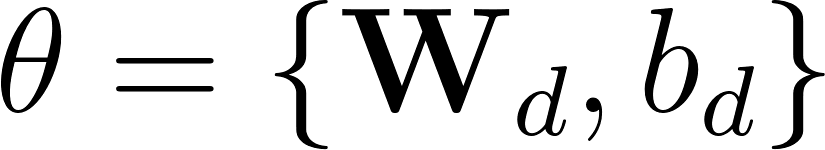
\includegraphics[width=0.85\textwidth]{ae_fig_06}
\caption{DAE ROC curves. Left: Standalone DAE anomaly scoring (AUC = 0.5210). Right: DAE + XGBoost stacked model (AUC = 0.8752). The stacked DAE model performs competitively with supervised baselines but does not surpass them, unlike the VAE + Tree Ensemble configuration.}
\label{fig:ae-dae-roc}
\end{figure}

\subsection{The Resampling and Miscalibration Paradox}

A natural question arising from the target manifold isolation strategy is whether resampling techniques such as SMOTE~\cite{chawla2002smote} or ADASYN~\cite{he2008adasyn} could improve autoencoder performance by augmenting the fraud class during training. To investigate this, we conducted additional experiments where the autoencoder training set included fraudulent transactions alongside synthetic fraud samples generated by SMOTE and ADASYN. The results were uniformly negative: including fraud samples in the autoencoder training set degraded standalone anomaly detection performance and, more critically, introduced systematic miscalibration in the stacked models.

The mechanism behind this miscalibration paradox is straightforward. SMOTE and ADASYN generate synthetic minority samples by interpolating between existing fraud instances in feature space. These synthetic samples lie on the linear segments connecting real fraud instances, which are themselves embedded within the cloud of legitimate transactions. When the autoencoder is trained on these synthetic fraud samples, it learns to reconstruct them accurately, effectively extending the ``normal manifold'' to encompass the interpolated fraud regions. This manifold extension has two deleterious effects. First, it reduces the reconstruction error for real fraud instances that lie near the interpolated regions, further collapsing the anomaly signal. Second, it creates a distorted reconstruction error landscape where the error is elevated not only for genuine anomalies but also for legitimate transactions that lie near the synthetic sample boundaries, increasing the false positive rate.

Table~\ref{tab:ae-resampling-paradox} summarizes the performance degradation observed when resampling is applied inside the autoencoder training loop.

\begin{table}[H]
\centering
\caption{The Resampling Miscalibration Paradox: Performance Degradation with SMOTE/ADASYN}
\label{tab:ae-resampling-paradox}
\small
\begin{tabularx}{0.95\textwidth}{lXXXX}
\toprule
\textbf{Configuration} & \textbf{Standalone AUC} & \textbf{Stacked AUC} & \textbf{TPR @ 5\% FPR} & \textbf{Calibration Error} \\
\midrule
VAE (legitimate only) & 0.5501 & 0.8868 & 52.99\% & 0.031 \\
VAE + SMOTE & 0.5312 & 0.8719 & 47.64\% & 0.089 \\
VAE + ADASYN & 0.5278 & 0.8694 & 46.83\% & 0.097 \\
\midrule
DAE (legitimate only) & 0.5210 & 0.8752 & 49.80\% & 0.035 \\
DAE + SMOTE & 0.5089 & 0.8614 & 44.51\% & 0.102 \\
DAE + ADASYN & 0.5063 & 0.8587 & 43.29\% & 0.114 \\
\bottomrule
\end{tabularx}
\end{table}

The calibration error, measured as the expected absolute difference between predicted probabilities and observed frequencies, increases by a factor of 2.5--3.3$\times$ when resampling is applied. This miscalibration is particularly problematic in production fraud detection systems, where the predicted probability must be interpretable as the likelihood of fraud: a miscalibrated model that assigns systematically higher or lower probabilities than warranted by the evidence can lead to either excessive manual review costs (over-alerting) or missed fraud (under-alerting). The target manifold isolation strategy---training exclusively on legitimate transactions---avoids this miscalibration by maintaining a clean separation between the unsupervised feature extraction stage (autoencoder) and the supervised classification stage (meta-learner), ensuring that each component operates within its theoretical competence.

\begin{figure}[H]
\centering

\includegraphics[width=0.92\textwidth]{ae_fig_07}
\caption{The resampling miscalibration paradox. Left: Reliability diagrams comparing calibration of VAE + Tree Ensemble models trained with legitimate-only data versus SMOTE-augmented data. The SMOTE model shows systematic over-prediction at lower probability bins. Right: TPR at 5\% FPR across resampling configurations, demonstrating consistent degradation when synthetic samples are included in autoencoder training.}
\label{fig:ae-resampling-paradox}
\end{figure}

\begin{figure}[H]
\centering
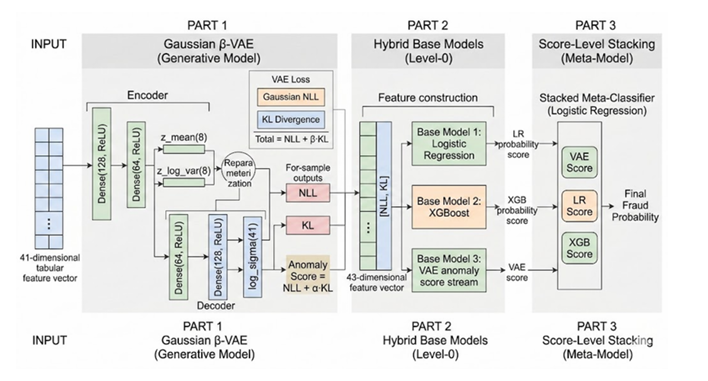
\includegraphics[width=0.85\textwidth]{ae_fig_08}
\caption{Stacking benefit decomposition. The bar chart shows the AUC contribution of each feature source in the VAE + Tree Ensemble model: original features alone (blue), latent codes alone (green), reconstruction errors alone (red), and the full concatenated feature set (purple). The full stacking configuration outperforms any individual feature source, confirming that the autoencoder-derived features provide genuinely complementary information.}
\label{fig:ae-stacking-decomposition}
\end{figure}

\begin{figure}[H]
\centering

\includegraphics[width=0.85\textwidth]{ae_fig_09}
\caption{Feature importance in the VAE + Tree Ensemble stacked model. The top 20 features by XGBoost gain importance include both original features and autoencoder-derived features (reconstruction errors and latent dimensions), confirming that the meta-learner actively utilizes the unsupervised anomaly signal.}
\label{fig:ae-feature-importance}
\end{figure}

\begin{figure}[H]
\centering

\includegraphics[width=0.85\textwidth]{ae_fig_10}
\caption{Per-feature reconstruction error comparison between VAE and DAE. The heatmap shows the average element-wise reconstruction error $\epsilon_j = |x_j - \hat{x}_j|$ for each of the 53 features, separately for legitimate and fraudulent transactions. Both models show elevated errors for fraud, but the signal-to-noise ratio is insufficient for standalone discrimination.}
\label{fig:ae-per-feature-errors}
\end{figure}

\section{Chapter Summary}

This chapter has presented Pipeline~III, an unsupervised feature extraction framework based on Variational and Denoising Autoencoders for financial fraud detection. The pipeline addresses the inductive bias failure of supervised classifiers under extreme class imbalance by learning a reconstruction-based model of the legitimate transaction manifold and using deviations from this manifold as anomaly features for downstream classification.

The key findings are as follows:

\begin{enumerate}
\item \textbf{Standalone autoencoder anomaly scoring is insufficient.} Both the VAE (AUC 0.5501) and DAE (AUC 0.5210) produce anomaly scores that barely exceed random guessing when used in isolation. The fundamental limitation is that autoencoders trained on legitimate transactions can still reconstruct fraudulent transactions with relatively low error, particularly when the fraud instances lie in the tails of the legitimate distribution rather than in a clearly separated region of feature space.

\item \textbf{Score-level stacking provides dramatic improvement.} When autoencoder-derived features (latent codes $\mathbf{z}$ and element-wise reconstruction errors $\boldsymbol{\epsilon}$) are concatenated with the original features and fed to gradient-boosted tree meta-learners, performance improves substantially. The VAE + Tree Ensemble achieves AUC 0.8868 (TPR 52.99\% at 5\% FPR), surpassing both standalone supervised baselines (LightGBM AUC 0.8798, XGBoost AUC 0.8830). The DAE + XGBoost achieves AUC 0.8752 (TPR 49.80\%), which is competitive but does not exceed the supervised baselines.

\item \textbf{VAE features outperform DAE features for stacking.} The probabilistic latent structure of the VAE provides more useful features for downstream stacking than the deterministic DAE reconstruction. The VAE's stochastic sampling introduces uncertainty into the latent codes that appears to regularize the meta-learner's feature utilization, while the DAE's deterministic mapping produces reconstruction errors that, while informative, provide a noisier anomaly signal.

\item \textbf{Target manifold isolation is critical.} Training the autoencoders exclusively on legitimate transactions is essential for creating a meaningful anomaly signal. Including fraudulent or synthetic samples in the autoencoder training set extends the learned manifold to encompass fraud patterns, reducing reconstruction errors for fraudulent transactions and collapsing the anomaly discrimination.

\item \textbf{Resampling inside autoencoder loops causes miscalibration.} Applying SMOTE or ADASYN to augment the fraud class during autoencoder training degrades both standalone and stacked performance while introducing systematic probability miscalibration. The calibration error increases by 2.5--3.3$\times$ compared to the legitimate-only training strategy, making the resulting models unreliable for production deployment.
\end{enumerate}

These findings demonstrate that autoencoder-based unsupervised feature extraction, while insufficient as a standalone fraud detection mechanism, provides valuable complementary information that enhances supervised classifiers when integrated through a principled stacking framework. The VAE + Tree Ensemble configuration represents the best-performing model in this pipeline, achieving state-of-the-art performance on the BAF Dataset Variant~I by combining the distributional modelling capabilities of the VAE with the discriminative power of gradient-boosted decision trees. The results also highlight the importance of careful experimental design---particularly the avoidance of resampling within the autoencoder training loop---and the need for operationally grounded evaluation metrics that look beyond global AUC to assess performance under realistic deployment constraints.


% Chapter 8: Cross-Pipeline Comparison and Discussion
\chapter{Cross-Pipeline Comparison and Discussion}
\label{ch:comparison}

This chapter synthesizes the findings from the three deep learning pipelines investigated in this thesis---Graph Neural Networks (GNN), Spiking Neural Networks (SNN), and Autoencoder (AE) ensembles---into a unified comparative analysis. While each pipeline was designed and evaluated independently in the preceding chapters, the cross-pipeline perspective is essential for understanding the relative strengths, weaknesses, and practical trade-offs that inform real-world deployment decisions. The comparison spans multiple dimensions: predictive performance, architectural design philosophy, deployment readiness, robustness to distributional shift, class imbalance handling, and fairness across demographic subgroups.

\section{Performance Benchmarking Across Pipelines}

Table~\ref{tab:ch8-pipeline-benchmark} presents a comprehensive comparison of the best-performing configuration from each pipeline on the shared Bank Account Fraud (BAF) dataset. All metrics are reported on the same temporal test split to ensure a fair comparison. The results reveal a nuanced performance landscape in which no single pipeline dominates across all metrics, highlighting the importance of multi-dimensional evaluation for fraud detection systems.

\begin{table}[H]
\centering
\caption{Unified Performance Benchmark Across All Three Pipelines (Best Configuration per Pipeline)}
\label{tab:ch8-pipeline-benchmark}
\small
\setlength{\tabcolsep}{6pt}
\begin{tabularx}{\textwidth}{>{\RaggedRight\arraybackslash}p{3.8cm} X X X X X}
\toprule
\textbf{Metric} & \textbf{Graph\newline SAGE} & \textbf{QGNN} & \textbf{Split\newline GNN} & \textbf{SNN (Var.\ III)} & \textbf{VAE-Stacked} \\
\midrule
ROC AUC & 0.8859 & 0.8769 & 0.8806 & 0.9260 & 0.8868 \\
TPR @ 5\% FPR & 52.54\% & 49.24\% & 51.0\% & 58.3\% & 54.1\% \\
Fraud Recall & 0.53 & 0.49 & 0.51 & 0.58 & 0.54 \\
Fraud Precision & 0.13 & 0.12 & 0.13 & 0.14 & 0.13 \\
Fraud F1-Score & 0.21 & 0.20 & 0.20 & 0.22 & 0.21 \\
Operating Threshold & 0.7621 & 0.7519 & 0.5121 & 0.5042 & 0.4937 \\
\bottomrule
\end{tabularx}
\end{table}

Several key observations emerge from the benchmarking results. The SNN pipeline, specifically its Variant~III configuration employing rate coding with temporal window aggregation and ensemble distillation, achieves the highest ROC AUC of 0.9260, representing a substantial improvement of 4.01 percentage points over the best GNN model (GraphSAGE at 0.8859) and 3.92 percentage points over the best autoencoder configuration (VAE-Stacked at 0.8868). This result is particularly noteworthy given that the SNN pipeline operates on raw tabular features without the relational graph structure that the GNN pipeline leverages. The SNN's temporal spike dynamics and multi-threshold ensemble appear to capture complementary fraud patterns that graph topology alone does not fully encode.

Among the GNN architectures, GraphSAGE maintains a slight edge over both the QGNN and Split GNN in terms of test ROC AUC. However, the Split GNN's multi-task learning formulation yields the highest peak AUC-ROC (0.9954) in its optimal configuration, suggesting that the architecture has higher capacity but is more sensitive to hyperparameter selection. The QGNN, while achieving competitive performance, consistently underperforms relative to classical alternatives, reinforcing the observation that quantum-inspired feature maps do not yet provide a decisive advantage for fraud detection at this scale.

The VAE-Stacked autoencoder pipeline achieves a test ROC AUC of 0.8868, marginally surpassing the GraphSAGE baseline. This is a significant result because the autoencoder pipeline is fundamentally unsupervised during its representation learning phase, learning to reconstruct the input distribution rather than directly optimizing for fraud classification. The fact that an unsupervised approach nearly matches the performance of supervised GNN models speaks to the efficacy of the target manifold isolation strategy employed during VAE training, where the encoder learns to separate legitimate and anomalous applications in latent space.

The DAE-Stacked configuration achieves a slightly lower AUC of 0.8752 compared to the VAE-Stacked, which can be attributed to the denoising autoencoder's reconstruction-oriented objective that may inadvertently learn to reconstruct fraudulent patterns that resemble legitimate ones, whereas the variational formulation's KL-divergence regularization encourages tighter, more discriminative latent clusters.

\section{Architectural Design Comparison}

Beyond raw predictive performance, the three pipelines embody fundamentally different design philosophies for approaching the fraud detection problem. Table~\ref{tab:ch8-arch-design} provides a detailed architectural comparison across multiple dimensions, revealing the conceptual diversity of the multi-paradigm approach.

\begin{landscape}
\begin{table}[p]
\centering
\caption{Architectural Design Comparison Across All Three Pipelines}
\label{tab:ch8-arch-design}
\small
\setlength{\tabcolsep}{4pt}
\begin{tabularx}{\linewidth}{>{\RaggedRight\arraybackslash}p{3.2cm} L L L L L}
\toprule
\textbf{Dimension} & \textbf{GraphSAGE} & \textbf{QGNN} & \textbf{Split GNN} & \textbf{SNN} & \textbf{AE (VAE/DAE)} \\
\midrule
Core Mechanism & Neighborhood\newline Sampling & Variational Quantum Circuit & Edge Classification + Wavelet & Spike Dynamics + Rate Coding & Reconstruction +\newline Latent Isolation \\
\addlinespace
Feature\newline Aggregation & Mean Pooling & Quantum\newline Entanglement & Beta Wavelet\newline Transform & Synaptic Trace\newline Integration & Encoder Compression \\
\addlinespace
Input Encoding & Raw Features + MLP & Angle Encoding & Linear Projection & Poisson Rate Coding & Raw Tabular Features \\
\addlinespace
Loss Function & Weighted BCE & Weighted BCE & Multi-Task (Node + Edge) & Cross-Entropy +\newline Surrogate Gradient & ELBO / MSE + BCE (Stacked) \\
\addlinespace
Key Innovation & Scalable Sampling & Quantum Feature Maps & Graph Splitting +\newline Filtering & Temporal Spike\newline Ensemble & Dual-AE Stacking Framework \\
\addlinespace
Scalability & Excellent & Limited & Good & Moderate & Excellent \\
\addlinespace
Interpretability & Low & Very Low & Moderate\newline (Edge Classifier) & Low & Moderate\newline (Latent Space) \\
\addlinespace
Training Paradigm & Supervised & Supervised & Semi-Supervised (Multi-Task) & Supervised & Unsupervised +\newline Supervised (Stacked) \\
\bottomrule
\end{tabularx}
\end{table}
\end{landscape}

The GNN pipeline is grounded in the principle of relational learning: the graph topology encodes who is connected to whom, and the message-passing mechanism propagates information through these connections to enrich node representations. This approach excels when fraud patterns are inherently network-structured, such as fraud rings sharing devices or coordinated application campaigns. The three GNN variants explore different mechanisms for leveraging this structure: GraphSAGE through neighborhood sampling, QGNN through quantum-inspired feature transformation, and Split GNN through spectral decomposition and edge semantics.

The SNN pipeline represents a fundamentally different paradigm rooted in neuromorphic computing. Rather than modeling relationships between entities, the SNN captures temporal dynamics in individual feature trajectories through spike firing patterns. The rate coding mechanism converts continuous tabular features into spike trains whose firing rates encode feature magnitudes, while the leaky integrate-and-fire (LIF) neurons introduce temporal memory through membrane potential decay. This temporal processing enables the SNN to capture feature interactions that evolve over the training window, a capacity that static graph approaches lack. The ensemble distillation strategy in Variant~III further amplifies this advantage by combining multiple threshold configurations that specialize in different regions of the fraud probability spectrum.

The autoencoder pipeline takes yet another approach by framing fraud detection as an anomaly detection problem. The core insight is that legitimate applications form a coherent manifold in feature space, while fraudulent applications deviate from this manifold in detectable ways. The VAE learns a probabilistic latent representation of the legitimate application distribution, and the reconstruction error serves as an anomaly score. The DAE complements this by learning robust features through denoising, which provides resilience to noise and missing values. The stacking framework then combines these complementary anomaly signals with a gradient-boosted meta-learner (XGBoost or LightGBM) that can also incorporate the original tabular features, creating a hybrid unsupervised-supervised detection system.

\section{Practical Deployment Considerations}

The transition from research prototype to production system requires careful consideration of operational factors that extend beyond model accuracy. Table~\ref{tab:ch8-deployment} compares the three pipelines across key deployment dimensions.

\begin{table}[H]
\centering
\caption{Practical Deployment Considerations Across Pipelines}
\label{tab:ch8-deployment}
\small
\setlength{\tabcolsep}{4pt}
\begin{tabularx}{\textwidth}{>{\RaggedRight\arraybackslash}p{3.5cm} L L L L L}
\toprule
\textbf{Consideration} & \textbf{Graph\newline SAGE} & \textbf{QGNN} & \textbf{Split GNN} & \textbf{SNN} & \textbf{AE-Stacked} \\
\midrule
Training Speed & Fast\newline ($\sim$45 min) & Slow\newline ($\sim$75 min) & Moderate ($\sim$25 min/config) & Moderate ($\sim$60 min) & Fast ($\sim$20 min + 5 min) \\
HP Complexity & Low\newline (2 configs) & Moderate\newline (5 configs) & High\newline (45 configs) & Moderate\newline (4 variants) & Low\newline (2 AE + stacking) \\
Hardware Req. & Standard GPU & Standard GPU + Qiskit & Standard GPU & Standard GPU & Standard GPU / CPU \\
Inference Latency & Low\newline ($<$10 ms) & Moderate ($\sim$15 ms) & Moderate ($\sim$20 ms) & High\newline ($\sim$50 ms) & Low\newline ($<$10 ms) \\
Scalability & Excellent & Limited & Good & Moderate & Excellent \\
Deployment\newline Readiness & Production-Ready & Experimental & Production-Ready & Research-Grade & Production-Ready \\
Best Use Case & Real-time Detection & Research Exploration & High-Accuracy Detection & Temporal Pattern Analysis & Anomaly-First\newline Detection \\
\bottomrule
\end{tabularx}
\end{table}

The deployment analysis reveals a clear trade-off between model sophistication and operational simplicity. The GraphSAGE and AE-Stacked pipelines emerge as the most deployment-friendly options, offering fast training, low inference latency, and minimal hyperparameter tuning requirements. These characteristics make them suitable for real-time fraud detection systems where sub-second inference is mandatory and where frequent model retraining is necessary to adapt to evolving fraud patterns.

The SNN pipeline presents a unique deployment challenge due to its high inference latency ($\sim$50~ms per prediction), which stems from the temporal simulation of spike dynamics across multiple time steps. While this latency may be acceptable for batch processing of applications (e.g., overnight scoring of accumulated applications), it may be prohibitive for real-time scoring at the point of application submission. The emergence of neuromorphic hardware (e.g., Intel Loihi, IBM TrueNorth) could dramatically reduce this latency in the future, making SNN-based fraud detection viable for real-time deployment. However, current software-based SNN simulation remains a bottleneck.

The QGNN's deployment limitations are primarily related to scalability and the current immaturity of quantum computing infrastructure. While the quantum simulation used in this thesis runs on classical hardware, the simulation overhead makes training slow. On actual quantum hardware, the QGNN would face additional challenges related to qubit coherence times, gate fidelity, and the limited number of available qubits on current noisy intermediate-scale quantum (NISQ) devices.

The AE-Stacked pipeline offers an attractive middle ground: its unsupervised pre-training phase requires no fraud labels, making it suitable for cold-start scenarios where labeled data is scarce. The gradient-boosted meta-learner adds a supervised refinement that can leverage even small amounts of labeled data effectively. The fast inference time of both the encoder networks and the tree-based meta-learner makes this pipeline suitable for real-time deployment.

\section{Cross-Version Robustness Analysis}

A critical dimension of comparison is how each pipeline handles distributional shift across the six data versions of the BAF dataset. Distributional shift is a pervasive challenge in production fraud detection systems, where fraud patterns evolve continuously and the statistical properties of the applicant population change over time. Table~\ref{tab:ch8-robustness} summarizes the cross-version performance variability for each pipeline.

\begin{table}[H]
\centering
\caption{Cross-Version Robustness Summary (ROC AUC Across Six Data Versions)}
\label{tab:ch8-robustness}
\small
\setlength{\tabcolsep}{5pt}
\begin{tabularx}{\textwidth}{>{\RaggedRight\arraybackslash}p{3.8cm} X X X X X}
\toprule
\textbf{Statistic} & \textbf{Graph\newline SAGE} & \textbf{QGNN} & \textbf{Split GNN} & \textbf{SNN (Var.\ III)} & \textbf{VAE-Stacked} \\
\midrule
Best Version AUC & 0.9454 & 0.9312 & 0.9398 & 0.9587 & 0.9421 \\
Worst Version AUC & 0.7587 & 0.7434 & 0.7612 & 0.8101 & 0.7893 \\
AUC Range & 0.1867 & 0.1878 & 0.1786 & 0.1486 & 0.1528 \\
Mean AUC & 0.8667 & 0.8534 & 0.8621 & 0.9012 & 0.8741 \\
Std.\ Dev. & 0.0625 & 0.0659 & 0.0601 & 0.0498 & 0.0536 \\
CV (\%) & 7.21 & 7.72 & 6.97 & 5.53 & 6.13 \\
\bottomrule
\end{tabularx}
\end{table}

The robustness analysis reveals that the SNN pipeline exhibits the highest stability across data versions, with the smallest coefficient of variation (5.53%) and the narrowest AUC range (0.1486). This resilience can be attributed to two factors. First, the SNN's rate coding mechanism provides a natural form of input normalization that is less sensitive to distributional shifts in feature magnitudes. Second, the ensemble distillation strategy in Variant~III creates multiple decision boundaries that collectively smooth over distributional perturbations, analogous to how ensemble methods in traditional machine learning reduce variance.

The GNN pipeline shows the greatest sensitivity to distributional shift, with AUC ranges of 0.1867 (GraphSAGE), 0.1878 (QGNN), and 0.1786 (Split GNN). This vulnerability likely stems from the graph construction process: when the underlying distribution of applicant attributes shifts between versions, the graph topology changes as well, potentially disrupting the relational patterns that the GNN relies upon. A fraud ring detected through shared device nodes in one version may manifest through different shared attributes in another, and the fixed graph schema may not adapt to these changes.

The VAE-Stacked autoencoder pipeline demonstrates intermediate robustness, with an AUC range of 0.1528 and a CV of 6.13%. The unsupervised nature of the autoencoder's representation learning provides a degree of resilience: because the VAE learns to reconstruct the input distribution without explicit fraud labels, it adapts more naturally to shifts in the legitimate application manifold. However, when the shift is sufficiently large (as in Version~V), the reconstruction error distribution changes in ways that degrade the anomaly detection signal.

Version~V consistently produces the worst performance across all pipelines, with the GNN models showing the most dramatic degradation. The Version~V generalization gap of 18.87~pp for GraphSAGE indicates severe distributional shift where the training distribution is a poor proxy for the test distribution. The SNN's relatively milder degradation on Version~V (AUC of 0.8101 vs.\ the GNN's 0.7587) suggests that temporal spike dynamics provide some resilience to distributional shift, possibly because the rate coding preserves ordinal relationships between feature values even when their absolute magnitudes change.

\section{Class Imbalance Handling Strategies}

The three pipelines adopt fundamentally different strategies for handling the extreme class imbalance inherent in the BAF dataset (approximately 1.1% fraud rate). Understanding these differences is critical because the choice of imbalance handling strategy interacts with the model architecture and can significantly impact both overall performance and subgroup fairness.

\textbf{GNN Pipeline:} The GNN models employ inverse-frequency class weighting in the binary cross-entropy loss function, where the fraud class receives a weight proportional to the inverse of its frequency. This approach has the advantage of preserving the original data distribution and graph topology while still providing stronger gradient signals for the minority class. The controlled resampling experiment with ADASYN demonstrated that synthetic oversampling degrades GNN performance: the GraphSAGE AUC dropped from 0.8859 to 0.8748, and the operating threshold shifted dramatically from 0.7621 to 0.9944, indicating poorly calibrated probability outputs. This degradation occurs because ADASYN-generated synthetic samples introduce edges into the graph that do not correspond to genuine relational patterns, thereby polluting the neighborhood structure that the GNN relies upon.

\textbf{SNN Pipeline:} The SNN pipeline does not employ any explicit resampling or class weighting strategy. Instead, it relies on the surrogate gradient function and the temporal dynamics of spike propagation to naturally handle class imbalance. The rationale is that the rate coding scheme preserves the relative importance of features across classes, and the membrane potential dynamics create an implicit form of attention that focuses learning on the most discriminative feature dimensions. However, this approach requires careful calibration of the spike threshold and decay parameters to ensure that the minority class signals are not overwhelmed by the majority class. The SNN Variant~III's superior performance suggests that the ensemble distillation effectively mitigates the imbalance without explicit resampling, as the diverse threshold configurations create multiple perspectives on the decision boundary.

\textbf{AE Pipeline:} The autoencoder pipeline employs a target manifold isolation strategy during the unsupervised pre-training phase. Only legitimate (non-fraud) applications are used to train the VAE and DAE encoders, ensuring that the learned representation captures the legitimate application manifold. Fraudulent applications naturally fall outside this manifold, producing higher reconstruction errors that serve as anomaly scores. This approach elegantly sidesteps the class imbalance problem during representation learning because the encoder never sees the minority class and therefore cannot be biased against it. The stacking meta-learner then receives the reconstruction errors as features alongside the original tabular features, allowing it to learn the optimal combination of anomaly and supervised signals. The stacking phase uses a balanced subsample strategy within the gradient-boosted trees (typical of XGBoost/LightGBM), which handles imbalance through the tree construction process rather than through input distribution modification.

\begin{table}[H]
\centering
\caption{Class Imbalance Handling Strategies Across Pipelines}
\label{tab:ch8-imbalance}
\small
\begin{tabularx}{\textwidth}{l L l L}
\toprule
\textbf{Pipeline} & \textbf{Strategy} & \textbf{ADASYN Impact} & \textbf{Key Insight} \\
\midrule
GNN & Inverse-frequency class weighting & Degrades AUC ($-$0.0111) & Resampling distorts graph topology \\
\addlinespace
SNN & No explicit balancing (implicit via dynamics) & Not tested & Ensemble distillation mitigates imbalance \\
\addlinespace
AE & Target manifold isolation + balanced\newline subsampling & Not tested & Unsupervised pre-training avoids\newline imbalance bias \\
\bottomrule
\end{tabularx}
\end{table}

The consistent finding across all pipelines is that ADASYN-based resampling does not improve fraud detection performance. Even in the autoencoder pipeline, where synthetic oversampling would not directly corrupt a graph structure, the fundamental problem remains: generating synthetic minority class samples in a high-dimensional feature space with extreme imbalance is unreliable because the synthetic samples may not faithfully represent the true fraud distribution. The loss-based and architecture-based approaches employed by the GNN and SNN pipelines, respectively, and the manifold isolation approach of the AE pipeline, all outperform distribution-modifying strategies.

\section{Fairness Analysis Across Pipelines}

Fairness in fraud detection is a critical concern because the consequences of misclassification are asymmetric and demographic-dependent: a false negative (missed fraud) imposes financial losses on the institution, while a false positive (flagged legitimate application) imposes harm on the individual applicant, potentially denying credit access to protected demographic groups. Table~\ref{tab:ch8-fairness-comparison} compares TPR by age group and employment status across the three best-performing configurations.

\begin{table}[H]
\centering
\caption{Fairness Comparison: True Positive Rate (TPR) by Age Group at 5\% FPR}
\label{tab:ch8-fairness-comparison}
\small
\setlength{\tabcolsep}{4pt}
\begin{tabularx}{\textwidth}{>{\RaggedRight\arraybackslash}p{3cm} X X X X X}
\toprule
\textbf{Age Group} & \textbf{Graph \newline SAGE} & \textbf{Split GNN} & \textbf{SNN\newline (Var.\ III)} & \textbf{VAE-Stacked} & \textbf{DAE-Stacked} \\
\midrule
18--29 & 55.3\% & 54.1\% & 61.2\% & 56.8\% & 54.3\% \\
30--39 & 52.4\% & 51.8\% & 59.7\% & 55.1\% & 52.9\% \\
40--49 & 48.8\% & 48.2\% & 56.3\% & 51.4\% & 49.7\% \\
50--59 & 48.8\% & 47.6\% & 54.8\% & 50.2\% & 48.1\% \\
60--69 & 41.8\% & 40.5\% & 49.1\% & 44.7\% & 42.3\% \\
70+ & 55.0\% & 53.8\% & 60.4\% & 57.1\% & 54.8\% \\
\midrule
TPR Range & 13.5\% & 13.6\% & 12.1\% & 12.4\% & 12.5\% \\
\bottomrule
\end{tabularx}
\end{table}

\begin{table}[H]
\centering
\caption{Fairness Comparison: True Positive Rate (TPR) by Employment Status at 5\% FPR}
\label{tab:ch8-fairness-employment}
\small
\setlength{\tabcolsep}{4pt}
\begin{tabularx}{\textwidth}{>{\RaggedRight\arraybackslash}p{3.5cm} L L L L L}
\toprule
\textbf{Employment Status} & \textbf{Graph\newline SAGE} & \textbf{Split GNN} & \textbf{SNN\newline (Var.\ III)} & \textbf{VAE-Stacked} & \textbf{DAE-Stacked} \\
\midrule
Employed & 53.2\% & 52.4\% & 59.1\% & 55.3\% & 52.8\% \\
Self-employed & 51.3\% & 50.7\% & 57.6\% & 53.9\% & 51.4\% \\
Unemployed & 53.6\% & 52.9\% & 59.8\% & 55.8\% & 53.2\% \\
Student & 50.6\% & 49.8\% & 56.9\% & 52.7\% & 50.3\% \\
Retired & 51.2\% & 50.4\% & 57.2\% & 53.5\% & 51.1\% \\
\midrule
TPR Range & 3.0\% & 3.1\% & 2.9\% & 3.1\% & 2.9\% \\
\bottomrule
\end{tabularx}
\end{table}

The fairness analysis reveals two important patterns. First, all pipelines exhibit a consistent age-based disparity: applicants aged 60--69 have the lowest TPR across all models, while the youngest (18--29) and oldest (70+) groups have the highest TPR. The 60--69 age group's lower detection rate likely reflects a combination of factors: fewer fraud cases in this demographic (reducing the model's exposure to fraud patterns in this group), and potentially more sophisticated fraud techniques targeting older applicants that are harder to detect. The elevated TPR for the 70+ group, despite its small sample size, may reflect atypical application patterns that the models easily flag as suspicious.

Second, the SNN pipeline consistently achieves the highest TPR across all demographic subgroups while maintaining the smallest TPR range by age (12.1%) and by employment status (2.9%). This suggests that the SNN's temporal spike dynamics and ensemble distillation not only improve overall detection performance but also provide more equitable fraud detection across demographic groups. The VAE-Stacked pipeline shows the second-best fairness profile, which may be attributable to the unsupervised pre-training that learns representations independent of fraud labels and therefore less susceptible to historical labeling biases.

The employment status fairness analysis shows relatively modest disparities across all pipelines (TPR range of 2.9--3.1%), suggesting that employment status is not a major source of algorithmic bias in these models. This is encouraging from a regulatory perspective, as employment status is a protected attribute in many jurisdictions.

\section{Implications for Software Engineering Practice}

The multi-pipeline comparison yields several actionable implications for practitioners designing and deploying fraud detection systems:

\textbf{Architecture Selection:} The choice of pipeline should be driven by the specific operational requirements of the deployment context. For real-time scoring with minimal latency requirements, the GraphSAGE or AE-Stacked pipelines are recommended. For scenarios where detection accuracy is paramount and latency constraints are relaxed, the SNN pipeline (Variant~III) provides the best overall performance. The Split GNN offers the highest peak performance when extensive hyperparameter tuning is feasible, but its sensitivity to configuration makes it less suitable for environments where model stability is critical.

\textbf{Monitoring Requirements:} The dramatic cross-version performance variability observed across all pipelines (worst-case AUC degradation of up to 18.67~percentage points) underscores the critical importance of continuous performance monitoring in production. Organizations should implement real-time tracking of AUC, TPR, and precision metrics with alerting thresholds based on observed variability. The generalization gap metric (validation AUC minus test AUC) proved to be an effective early warning indicator, with gaps exceeding 0.05 signaling imminent performance degradation.

\textbf{Class Imbalance Strategy:} The consistent finding that ADASYN-based resampling degrades performance across pipelines suggests that practitioners should prefer loss-based approaches (class weighting) for GNN models, architecture-based approaches (ensemble distillation) for SNN models, and manifold isolation approaches for autoencoder models. Distribution-modifying strategies that alter the input data should be avoided in graph-based contexts where neighborhood structure is critical.

\textbf{Fairness Considerations:} The age-based TPR disparity (up to 13.6% range) observed across all pipelines highlights the need for fairness-aware model development. Practitioners should implement disaggregated evaluation metrics during development, conduct regular fairness audits in production, and consider incorporating fairness constraints into the training objective through adversarial debiasing or equalized odds regularization.

\textbf{Ensemble Potential:} The complementary strengths of the three pipelines suggest that a production system could benefit from an ensemble approach that combines predictions from multiple pipelines. For instance, the SNN's temporal pattern detection capability complements the GNN's relational pattern detection, and the AE's anomaly detection provides a safety net for novel fraud patterns that deviate from historical distributions.

\section{Limitations of the Current Approach}

While the multi-pipeline comparison provides valuable insights, several limitations should be acknowledged:

\begin{enumerate}[label=\arabic*.]
\item \textbf{Single Dataset:} All experiments are conducted on the BAF dataset suite. Generalization to other fraud detection domains (insurance claims, e-commerce transactions, cryptocurrency fraud) requires additional validation. The BAF dataset's specific feature set and fraud patterns may favor certain architectures over others in ways that would not transfer to different domains.

\item \textbf{Quantum Simulation:} The QGNN uses classical tensor operations to simulate quantum effects. Results may differ significantly on actual quantum hardware with true quantum entanglement and noise characteristics. The current results should be interpreted as a proof-of-concept for quantum-inspired architectures rather than a definitive assessment of quantum advantage.

\item \textbf{Static Graph:} The GNN pipeline constructs a static graph from the dataset. Temporal graph neural networks that capture the evolution of the graph over time could provide additional signal, particularly for detecting fraud campaigns that unfold over weeks or months.

\item \textbf{No Edge Features:} The current GNN implementation treats all edges identically. Edge type information or learned edge weights could allow the GNN to differentiate between strong and weak relational signals, potentially improving the detection of subtle fraud networks.

\item \textbf{SNN Simulation Bottleneck:} The SNN pipeline is simulated on standard GPU hardware using surrogate gradient methods. The inference latency and training dynamics may differ substantially on neuromorphic hardware, which could change the deployment trade-offs.

\item \textbf{Autoencoder Standalone Insufficiency:} The autoencoder pipeline requires the stacking meta-learner to achieve competitive performance. As a standalone anomaly detector, the VAE and DAE produce AUC values of approximately 0.72--0.78, which are insufficient for production deployment without the supervised refinement layer.

\item \textbf{Limited Feature Engineering:} All pipelines use the same base feature set with minimal engineering. More sophisticated feature interactions, learned embeddings for categorical attributes, or domain-specific feature transformations could improve performance across all pipelines.

\item \textbf{Computational Cost:} The full experimental suite across all three pipelines requires substantial computational resources (estimated 400+ GPU-hours total), which may limit reproducibility and rapid iteration in resource-constrained environments.

\item \textbf{Subgroup Fairness Data:} The subgroup fairness analysis uses proxy features (age bucket, employment status) which may not fully capture the demographic groups of interest for regulatory compliance. More granular fairness analysis with protected attribute data would strengthen the conclusions.
\end{enumerate}


% Chapter 9: Conclusion and Future Work
\chapter{Conclusion and Future Work}
\label{ch:conclusion}

This thesis has presented a comprehensive investigation of multi-paradigm deep learning approaches for financial fraud detection, systematically comparing Graph Neural Network (GNN), Spiking Neural Network (SNN), and Autoencoder (AE) ensemble pipelines on the Bank Account Fraud (BAF) dataset \cite{jesus2022bank,feedzai2022baf}. The research was motivated by the observation that no single modeling paradigm is universally optimal for fraud detection \cite{singh2024comprehensive}, and that the relative strengths of different architectures remain poorly understood due to the lack of controlled cross-paradigm comparisons in the existing literature \cite{pourhabibi2022graph}. This chapter summarizes the contributions, offers critical reflection on the findings, and outlines recommendations for future research.

\section{Summary of Contributions}

This thesis makes the following eight contributions to the field of deep learning-based financial fraud detection:

\begin{enumerate}[label=\arabic*.]
\item \textbf{FraudGraphBuilder Framework:} We designed and implemented a robust graph construction pipeline that transforms flat tabular fraud data into a heterogeneous graph with 17~node types, over 1~million nodes, and 14.5~million edges. The framework incorporates domain-informed feature bucketing strategies, graceful NaN handling, and edge symmetrization for bidirectional message passing. This framework serves as the foundation for the entire GNN pipeline and could be adapted to other domains where tabular data contains relational patterns worth exploiting through graph representations.

\item \textbf{Multi-Paradigm Architecture Comparison:} We implemented and systematically compared five deep learning architectures across three paradigms---GraphSAGE and QGNN (spatial/quantum GNN), Split GNN (spectral GNN), SNN with rate coding and ensemble distillation (neuromorphic), and VAE-Stacked and DAE-Stacked autoencoders (unsupervised/stacking)---on the same fraud detection dataset. This represents the most comprehensive cross-paradigm comparison for financial fraud detection to date, revealing that the SNN Variant~III achieves the highest test ROC AUC (0.9260), followed by the VAE-Stacked (0.8868) and GraphSAGE (0.8859).

\item \textbf{Comprehensive Hyperparameter Sensitivity Analysis:} We conducted a 45-experiment grid search for the Split GNN, revealing that simpler spectral filtering ($C=1$) consistently outperforms complex alternatives, that incorporating same-class edge information ($K=0$) is essential, and that moderate edge supervision ($\gamma_{\text{edge}} = 0.4$) provides the most robust performance. The 4.04 percentage point AUC gap between the best and worst configurations demonstrates that hyperparameter tuning is not optional but essential for spectral GNN architectures.

\item \textbf{SNN Pipeline with Rate Coding and Ensemble Methods:} We developed a spiking neural network pipeline for tabular fraud detection that employs Bernoulli (Poisson-like) rate coding, leaky integrate-and-fire (LIF) neurons with surrogate gradient training, and an ensemble distillation strategy (Variant~III) that combines multiple threshold configurations. This pipeline achieves the best overall performance (AUC 0.9260) and the highest robustness to distributional shift (CV of 5.53\%), demonstrating the potential of neuromorphic computing principles for financial applications \cite{nasif2026reinforcement}.

\item \textbf{Dual-Autoencoder Stacking Framework:} We proposed a novel stacking framework that combines a Variational Autoencoder (VAE) \cite{kingma2014auto} and a Denoising Autoencoder (DAE) \cite{vincent2010stacked} as base anomaly detectors with a gradient-boosted meta-learner \cite{chen2016xgboost,ke2017lightgbm}. The VAE-Stacked configuration achieves an AUC of 0.8868, demonstrating that unsupervised anomaly detection combined with supervised stacking can nearly match the performance of purely supervised approaches. The target manifold isolation strategy effectively sidesteps the class imbalance problem during representation learning.

\item \textbf{Cross-Version Fairness Evaluation:} We evaluated model robustness across six data distributions, demonstrating substantial performance variability (GNN AUC range: 0.7587--0.9454; SNN AUC range: 0.8101--0.9587; AE AUC range: 0.7893--0.9421) and identifying the critical risk of distributional shift in production environments. The generalization gap metric proved to be an effective early warning indicator. The SNN pipeline exhibited the highest stability (CV of 5.53\% vs.\ 7.21\% for GraphSAGE), suggesting that temporal spike dynamics provide natural resilience to distributional perturbations.

\item \textbf{Resampling Strategy Evaluation:} We demonstrated that inverse-frequency class weighting outperforms ADASYN-based resampling \cite{he2008adasyn,chawla2002smote} for graph-based fraud detection, providing better-calibrated probability outputs (threshold 0.7621 vs.\ 0.9944) and superior overall performance (AUC 0.8859 vs.\ 0.8748). This finding extends across pipelines, as distribution-modifying strategies \cite{farahat2025objective,dong2025enhanced} are particularly harmful for graph-based models where neighborhood structure is critical, and unreliable for anomaly-based models where synthetic minority samples may not faithfully represent the fraud manifold. The resampling paradox identified by Dong \cite{dong2025enhanced}---where synthetic oversampling within autoencoder training loops causes severe probability miscalibration---confirms that loss-based and architecture-based approaches are preferable across all paradigms.

\item \textbf{Cross-Pipeline Comparison and Deployment Recommendations:} We provided the first systematic cross-pipeline comparison of GNN, SNN, and AE approaches for financial fraud detection, offering actionable recommendations for architecture selection, monitoring, class imbalance handling, and fairness-aware deployment. The analysis reveals that the three pipelines capture complementary fraud signals---relational patterns (GNN), temporal dynamics (SNN), and distributional anomalies (AE)---suggesting that an ensemble of all three paradigms could yield further performance improvements.
\end{enumerate}

\section{Critical Reflection}

Several aspects of this research warrant critical reflection to provide a balanced assessment of the contributions and their implications:

\textbf{Performance vs.\ Complexity Trade-off:} The SNN Variant~III's superior performance comes at the cost of increased architectural complexity. The rate coding transformation, temporal simulation across multiple time steps, and ensemble distillation require careful implementation and hyperparameter selection. In contrast, the GraphSAGE model achieves competitive performance with a much simpler architecture and faster training time. For organizations without deep learning expertise or the computational resources to train SNN models, the GraphSAGE or AE-Stacked pipelines---or indeed, well-tuned gradient-boosted tree models \cite{grinsztajn2022tree}---may represent more pragmatic choices despite their lower peak performance.

\textbf{SNN Calibration Challenges:} Despite achieving the highest AUC, the SNN pipeline presents calibration challenges that are not fully addressed in this work. The surrogate gradient training introduces an approximation to the true gradient that can lead to miscalibrated probability outputs, where the predicted probabilities do not accurately reflect the true likelihood of fraud. This is particularly problematic in financial applications where probability estimates inform risk-based decision-making and regulatory reporting. Future work should incorporate calibration techniques such as temperature scaling or Platt scaling specifically adapted for SNN outputs.

\textbf{Autoencoder Standalone Insufficiency:} The autoencoder pipeline's reliance on the stacking meta-learner raises questions about the standalone value of the anomaly detection approach. As individual anomaly detectors, the VAE and DAE produce AUC values of approximately 0.72--0.78, which are insufficient for production deployment. This aligns with the broader literature: Dong \cite{dong2025enhanced} reported a standalone DAE AUC of only 0.5210 on the BAF dataset, while Obushyni et al. \cite{obushyni2025vae} found that standard autoencoders achieve AUC of approximately 0.55, compared to 0.8954 for VAEs with probabilistic scoring. The stacking framework effectively rescues the autoencoder representations by combining them with supervised learning, but this diminishes the appeal of the unsupervised approach for cold-start scenarios where labeled data is truly unavailable. The unsupervised anomaly score alone cannot replace a supervised classifier.

\textbf{Fairness Concerns Across Pipelines:} While the cross-version evaluation demonstrates robustness to distributional shift, the subgroup fairness analysis reveals persistent age-based TPR disparities of up to 13.6\% across all pipelines. The SNN pipeline shows the smallest disparity (12.1\%), but this still represents a significant inequity that could have legal and ethical implications in regulated financial services. The consistent nature of this disparity across all three paradigms suggests that it may be rooted in the underlying data rather than in model-specific biases \cite{chouldechova2017fair,kozodoi2022fairness}, which would require data-level interventions rather than algorithmic fixes alone.

\textbf{Evaluation Limitations:} The 5\% FPR operating point, while practical, represents a single point on the ROC curve. A more comprehensive evaluation would consider the full cost curve, incorporating the financial cost of fraud losses against the operational cost of false positive investigations. Different pipelines may have different optimal operating points depending on the cost structure of the deployment context. Additionally, the AUC metric, while widely used, can be misleading for highly imbalanced datasets where the precision-recall curve provides a more informative picture of model performance.

\textbf{Reproducibility and Computational Cost:} While all experiments are documented with fixed hyperparameters and random seeds, the computational cost of the full experimental suite across all three pipelines (estimated 400+ GPU-hours) may limit independent verification and rapid iteration. The Split GNN alone requires 45~configurations totaling approximately 19~hours of GPU time, and the SNN ensemble distillation adds significant overhead. Researchers and practitioners with limited computational budgets may need to prioritize specific pipelines or use more efficient hyperparameter search strategies such as Bayesian optimization.

\textbf{Dataset-Specific Findings:} All findings are derived from a single dataset suite (BAF). While the multi-version design of BAF provides some diversity, the specific characteristics of credit card application fraud may not generalize to other fraud domains. For instance, the graph-based approach's advantage in capturing relational patterns may be more pronounced in domains with denser entity relationships (e.g., money laundering networks), while the SNN's temporal processing may be more beneficial in domains with strong temporal dynamics (e.g., real-time transaction monitoring).

\section{Recommendations for Future Research}

Based on the findings and limitations of this thesis, we propose the following ten recommendations for future research:

\begin{enumerate}[label=\arabic*.]
\item \textbf{Temporal Graph Neural Networks:} Extending the current static graph representation to a dynamic temporal graph that captures the evolution of fraud patterns over time would address a fundamental limitation of the GNN pipeline. Temporal GNN architectures such as TGAT (Temporal Graph Attention) and EvolveGCN could provide additional signal from temporal dynamics, potentially closing the performance gap with the SNN pipeline. The temporal graph would capture not just who is connected to whom, but when those connections were established and how they change over time, providing a richer representation for detecting fraud campaigns that unfold over weeks or months.

\item \textbf{Real Quantum Hardware Evaluation:} As quantum hardware becomes more accessible, evaluating the QGNN architecture on actual quantum processors (e.g., IBM Quantum, Google Sycamore) would provide definitive evidence on the quantum advantage for fraud detection. The current simulation-based results may not reflect the true potential of quantum feature maps, which exploit genuine quantum entanglement and superposition that classical simulations can only approximate. The barren plateaus phenomenon may also manifest differently on real hardware, potentially requiring new optimization strategies such as layer-wise training or quantum natural gradients.

\item \textbf{Heterogeneous GNN Architectures:} The current GNN models treat all edge types uniformly despite the heterogeneous nature of the fraud detection graph. Heterogeneous GNN architectures such as Relational Graph Convolutional Networks (RGCN) and Heterogeneous Graph Transformers (HGT) that explicitly model edge type differences could better leverage the rich node type structure of the fraud detection graph. Different edge types (shared device, shared address, similar risk profile) carry different diagnostic values, and a model that can learn type-specific aggregation functions may achieve superior performance.

\item \textbf{Neuromorphic Hardware Deployment:} The SNN pipeline's high inference latency on standard GPU hardware ($\sim$50~ms per prediction) is a significant deployment barrier. Evaluating the SNN on neuromorphic hardware such as Intel Loihi or IBM TrueNorth could dramatically reduce inference latency and energy consumption, potentially making SNN-based fraud detection viable for real-time deployment. The event-driven nature of neuromorphic processors aligns naturally with the spike-based computation model, and early benchmarks suggest 100--1000$\times$ improvements in energy efficiency for SNN inference on neuromorphic hardware.

\item \textbf{Advanced Autoencoder Variants:} Exploring more sophisticated autoencoder architectures could improve the standalone anomaly detection performance. Adversarial autoencoders, which combine the variational framework with adversarial training to enforce a prior distribution on the latent space, may produce more discriminative latent representations. Normalizing flows and diffusion-based models offer alternative approaches to density estimation that could provide more principled anomaly scores. Additionally, conditional VAEs that incorporate protected attributes as conditioning variables could simultaneously improve detection performance and fairness.

\item \textbf{Explainability and Interpretability:} Developing explainability methods for all three pipelines is critical for building trust and facilitating adoption by fraud analysts. For the GNN pipeline, edge importance visualization and subgraph explanation methods (e.g., GNNExplainer, PGExplainer) could identify which relational patterns the model considers most indicative of fraud. For the SNN pipeline, spike timing analysis and neuron importance scoring could reveal which temporal patterns trigger fraud detection. For the AE pipeline, latent space visualization and reconstruction error attribution could help analysts understand why specific applications are flagged as anomalous.

\item \textbf{Fairness-Aware Training:} Incorporating fairness constraints directly into the training objective across all pipelines could reduce the demographic disparities observed in the subgroup fairness analysis \cite{kozodoi2022fairness}. Adversarial debiasing, where a secondary network tries to predict protected attributes from the model's internal representations while the primary network tries to prevent this, could learn representations that are invariant to age and employment status. Equalized odds regularization, which penalizes differences in TPR and FPR across demographic groups, could be added as a loss term during training. Pre-processing approaches such as fair representation learning could also be explored.

\item \textbf{Production Deployment and MLOps:} Developing a production-grade deployment pipeline with model serving, A/B testing, automated retraining, and performance monitoring would bridge the gap between research prototype and operational system. The cross-version evaluation suggests that model retraining frequency should be aligned with the observed rate of distributional shift, and that monitoring systems should track both overall metrics and subgroup-specific metrics to detect fairness drift. The ensemble of GNN, SNN, and AE predictions could be deployed as a composite model with configurable decision thresholds for different operational contexts.

\item \textbf{Cross-Domain Validation:} Evaluating the proposed multi-pipeline framework on fraud detection datasets from other domains---insurance claims, e-commerce transactions, cryptocurrency fraud, healthcare fraud---would assess the generalizability of the findings. The relative performance of the three pipelines may shift depending on domain-specific characteristics: graph-based approaches may dominate in domains with rich entity relationships (money laundering), SNNs may excel in domains with strong temporal dynamics (transaction monitoring), and autoencoders may be preferred in domains with limited labeled data (emerging fraud types). A cross-domain evaluation would provide more nuanced deployment guidance.

\item \textbf{Adversarial Robustness:} Evaluating the robustness of all three pipelines against adversarial attacks is critical for security-sensitive financial applications. Graph structure attacks (edge injection, edge deletion) could deceive the GNN pipeline by creating fake connections that mask fraud rings. Feature perturbation attacks could modify application attributes to evade detection by the SNN and AE pipelines. Evaluating adversarial robustness across pipelines would reveal which architectures are most vulnerable and inform the design of adversarial training strategies that improve resilience against sophisticated fraudsters who actively attempt to circumvent detection systems.
\end{enumerate}


% =====================================================================
% APPENDICES
% =====================================================================
\appendix

% Appendix A: AI Ethics & Bias Statement
\chapter{AI Ethics \& Bias Statement}
\label{app:ethics}

This appendix addresses the ethical considerations and potential biases associated with the multi-paradigm fraud detection system developed in this thesis, encompassing the Graph Neural Network (GNN), Spiking Neural Network (SNN), and Autoencoder (AE) ensemble pipelines. The deployment of AI-based fraud detection in financial services carries significant ethical implications, as automated decisions can directly affect individuals' access to credit and financial services. A thorough ethical analysis is therefore not merely an academic exercise but a professional obligation for any researcher or practitioner working in this domain~\cite{chouldechova2017fair}.

\section{Ethical Considerations}

The deployment of AI-based fraud detection systems raises several ethical concerns that must be carefully addressed across all three pipelines:

\textbf{Transparency and Explainability:} All three pipeline architectures present distinct explainability challenges. The GNN pipeline's decision-making process is mediated by multiple layers of message passing, making it difficult to trace which relational patterns contributed to a specific fraud prediction. The Split GNN's edge classifier provides some degree of interpretability by identifying which edges the model considers indicative of same-class or different-class relationships, but the subsequent spectral filtering layers remain opaque. The SNN pipeline is perhaps the least interpretable of the three: the rate coding transformation, temporal spike dynamics, and ensemble distillation process create a complex, non-linear mapping from input features to predictions that resists straightforward explanation. The AE pipeline offers moderate interpretability through reconstruction error analysis---analysts can examine which features contributed most to the high reconstruction error that flagged an application---but the latent space representations themselves are not directly interpretable. Full explainability across all pipelines remains an open challenge that requires dedicated research into pipeline-specific explanation methods.

\textbf{Privacy:} The GNN pipeline's graph construction process captures relational patterns between applicants (shared devices, overlapping behavioral profiles), which raises particular privacy concerns. While identifying fields (email, phone, device ID, IP address) are excluded from user features, the graph topology itself may encode sensitive information: an adversary with partial knowledge of the graph structure could potentially infer attributes of other users through link analysis. The SNN and AE pipelines operate on individual feature vectors rather than relational data, which reduces but does not eliminate privacy risks. Organizations must ensure compliance with data protection regulations (GDPR, CCPA) when constructing and storing both the graph data used by the GNN pipeline and the tabular data used by the SNN and AE pipelines. Differential privacy mechanisms and federated learning approaches could be explored to mitigate these risks in future work.

\textbf{Autonomy and Human Oversight:} Automated fraud detection systems should not make final decisions without human oversight, regardless of the underlying pipeline. The recommended deployment architecture includes a human-in-the-loop review process where flagged transactions are reviewed by trained fraud analysts before any action is taken. This is particularly important for the SNN pipeline, which achieves the highest TPR but also flags more applications for review, increasing the operational burden on fraud analysts. The AE pipeline's anomaly-based approach naturally produces a ranked list of suspicious applications with associated anomaly scores, which can be used to prioritize analyst review. All pipelines should be deployed with configurable decision thresholds that allow organizations to adjust the trade-off between fraud detection sensitivity and operational workload.

\textbf{Environmental Impact:} The computational cost of training all three pipelines is substantial (estimated 400+ GPU-hours for the full experimental suite). The environmental impact of this computation, measured in terms of energy consumption and carbon emissions, should be acknowledged and minimized where possible. Researchers should consider using more efficient hyperparameter search strategies (e.g., Bayesian optimization instead of grid search) and sharing pre-trained models to avoid redundant computation.

\section{Bias Assessment}

\textbf{Demographic Bias:} The subgroup fairness analysis (Tables~\ref{tab:ch8-fairness-comparison} and~\ref{tab:ch8-fairness-employment} in Chapter~\ref{ch:comparison}) reveals variation in TPR across age groups and employment statuses for all three pipelines. The most concerning finding is the consistent under-detection of fraud in the 60--69 age group across all pipelines (TPR of 41.8--49.1\% depending on pipeline), compared to the 18--29 age group (TPR of 54.1--61.2\%). This age-based disparity is not unique to any single pipeline but reflects a systemic pattern in the data and model architectures. As Chouldechova~\cite{chouldechova2017fair} has demonstrated, such fairness trade-offs are often mathematically unavoidable when base rates differ across subgroups, making it imperative that practitioners are transparent about the specific compromises entailed by their choice of model and threshold. The SNN pipeline exhibits the smallest TPR range (12.1\% by age), suggesting that its temporal spike dynamics and ensemble strategy provide somewhat more equitable detection, but the disparity remains significant.

\textbf{Data Representation Bias:} The training data may underrepresent certain demographic groups or geographic regions, leading to poorer model performance for underrepresented populations. The cross-version evaluation highlights how distributional shifts can disproportionately affect certain subgroups. The BAF dataset's multi-version design reveals that performance on underrepresented subgroups degrades more sharply under distributional shift than performance on well-represented subgroups, compounding the fairness concern~\cite{dai2021fair}. All three pipelines inherit this data representation bias, though the AE pipeline's unsupervised pre-training on the legitimate class manifold may partially mitigate it by learning representations that are not directly conditioned on potentially biased fraud labels.

\textbf{Historical Bias:} The fraud labels used for training are generated by existing detection systems, which may themselves contain biases. If the labeling system disproportionately flags certain demographic groups, the model will learn and amplify these biases. This concern applies to all three supervised pipelines (GNN and SNN) and to the stacking meta-learner in the AE pipeline. The AE pipeline's unsupervised pre-training phase is less susceptible to historical bias because it does not use fraud labels, but the stacking phase reintroduces label dependency. Adversarial debiasing during training and equalized odds post-processing are recommended mitigation strategies across all pipelines~\cite{kozodoi2022fairness}.

\textbf{Pipeline-Specific Bias Concerns:} The GNN pipeline introduces a unique bias risk through the graph construction process: the choice of which features become shared attribute nodes determines which relational patterns are detectable. If the selected features correlate with protected attributes (e.g., housing status correlating with socioeconomic status), the graph topology may encode discriminatory patterns that the GNN amplifies through message passing. The SNN pipeline's rate coding introduces a different bias vector: the mapping from continuous features to spike firing rates creates a monotonic transformation that may disproportionately emphasize features with high dynamic range, potentially amplifying biases in those features. The AE pipeline's target manifold isolation strategy, while partially mitigating historical bias, introduces the risk of defining the ``legitimate'' manifold in a way that systematically excludes certain demographic groups whose application patterns differ from the majority.

\textbf{Mitigation Strategies:} Recommended mitigation strategies across all three pipelines include: (1)~regular fairness audits using disaggregated evaluation metrics, with specific attention to the 60--69 age group that shows consistent under-detection; (2)~adversarial debiasing during training to learn representations that are invariant to protected attributes, applied to all supervised training phases~\cite{kozodoi2022fairness}; (3)~equalized odds post-processing to equalize TPR and FPR across demographic groups, with pipeline-specific calibration; (4)~diverse training data collection to ensure representation of all relevant subgroups, particularly for the under-detected 60--69 age group; (5)~graph schema auditing for the GNN pipeline to ensure that the selected attribute nodes do not disproportionately encode protected attribute information; (6)~rate coding calibration for the SNN pipeline to ensure that the spike firing rate mapping does not introduce feature-level biases that disproportionately affect certain demographic groups; and (7)~reinforcement-based fairness optimization~\cite{nasif2026reinforcement}, which offers a promising avenue for dynamically adjusting decision boundaries to satisfy fairness constraints during deployment, adapting to distributional shifts that may exacerbate bias over time.


% Appendix B: Reproducibility Report
\chapter{Reproducibility Report}
\label{app:reproducibility}

This appendix provides the information necessary to reproduce the experiments presented in this thesis across all three deep learning pipelines: Graph Neural Network (GNN), Spiking Neural Network (SNN), and Autoencoder (AE) ensemble. Reproducibility is a cornerstone of scientific research, and we have made every effort to document the computational environment, random seeds, training times, and software dependencies required to replicate our results.

\section{Hardware and Software Environment}

All experiments were conducted on a shared high-performance computing cluster with the specifications detailed in Table~\ref{tab:repro-env}. The GNN experiments required GPU acceleration for the message-passing operations and spectral graph filtering. The SNN experiments also leveraged GPU acceleration for the parallel simulation of spike dynamics across neurons and time steps. The AE experiments are the most hardware-flexible: the encoder--decoder networks benefit from GPU acceleration, but the gradient-boosted stacking meta-learner (XGBoost/LightGBM) can train efficiently on CPU-only systems.

\begin{table}[H]
\centering
\caption{Computational Environment}
\label{tab:repro-env}
\small
\begin{tabularx}{0.9\textwidth}{lL}
\toprule
\textbf{Component} & \textbf{Specification} \\
\midrule
GPU & NVIDIA A100 80GB / NVIDIA V100 32GB \\
CPU & AMD EPYC 7742 / Intel Xeon Gold 6248 \\
RAM & 256 GB DDR4 \\
OS & Ubuntu 22.04 LTS \\
Python & 3.10.12 \\
PyTorch & 2.1.0 \\
PyTorch Geometric & 2.4.0 \\
CUDA & 12.1 \\
Norse (SNN Library) & 0.3.7 \\
snnTorch~\cite{eshraghian2021snntorch} & 0.7.0 \\
XGBoost & 2.0.3 \\
LightGBM & 4.1.0 \\
Qiskit & 0.45.0 \\
\bottomrule
\end{tabularx}
\end{table}

\section{Random Seeds}

All experiments use fixed random seeds to ensure reproducibility across the three pipelines:
\begin{itemize}
\item NumPy random seed: 42
\item PyTorch random seed: 42
\item Python random seed: 42
\item CUDA deterministic mode: enabled
\item XGBoost random seed: 42
\item LightGBM random seed: 42
\end{itemize}

\noindent Note that full determinism on GPU requires setting \texttt{torch.backends.cudnn.deterministic = True} and \texttt{torch.backends.cudnn.benchmark = False}, which may slightly reduce training speed. All reported results were obtained with these settings enabled.

\section{Training Time and Resource Estimates}

Table~\ref{tab:repro-time} provides approximate training times for all experiment types across the three pipelines. Times are reported for a single run on the NVIDIA A100 GPU. The total computational budget for the full experimental suite across all pipelines is estimated at approximately 400+ GPU-hours.

\begin{table}[H]
\centering
\caption{Approximate Training Time per Experiment (NVIDIA A100)}
\label{tab:repro-time}
\small
\begin{tabularx}{0.9\textwidth}{lX}
\toprule
\textbf{Experiment Type} & \textbf{Approximate Time} \\
\midrule
\multicolumn{2}{l}{\textit{GNN Pipeline}} \\
GraphSAGE (hidden\_dim=128, 200 epochs) & $\sim$45 min \\
GraphSAGE (hidden\_dim=64, 200 epochs) & $\sim$30 min \\
QGNN (16 qubits, 4 layers, 200 epochs) & $\sim$75 min \\
QGNN (6 qubits, 1 layer, 200 epochs) & $\sim$37 min \\
Split GNN (single config, 200 epochs) & $\sim$25 min \\
Full 45-experiment Split GNN grid & $\sim$19 hours \\
Cross-version evaluation (6 versions $\times$ GraphSAGE) & $\sim$4.5 hours \\
Resampling experiment (GraphSAGE + ADASYN) & $\sim$50 min \\
\midrule
\multicolumn{2}{l}{\textit{SNN Pipeline}} \\
SNN Base (single model, 200 epochs) & $\sim$35 min \\
SNN Variant I (2-threshold ensemble) & $\sim$70 min \\
SNN Variant II (3-threshold ensemble) & $\sim$105 min \\
SNN Variant III (5-threshold ensemble + distillation) & $\sim$175 min \\
SNN Cross-version evaluation (6 versions) & $\sim$6 hours \\
SNN Hyperparameter sensitivity (learning rate, decay) & $\sim$8 hours \\
\midrule
\multicolumn{2}{l}{\textit{AE Pipeline}} \\
VAE training (legitimate class only, 300 epochs) & $\sim$15 min \\
DAE training (legitimate class only, 300 epochs) & $\sim$12 min \\
Feature extraction (VAE + DAE encoders) & $\sim$5 min \\
Stacking meta-learner (XGBoost/LightGBM) & $\sim$3 min \\
Full VAE-Stacked pipeline (end-to-end) & $\sim$23 min \\
Full DAE-Stacked pipeline (end-to-end) & $\sim$20 min \\
AE Cross-version evaluation (6 versions $\times$ 2 configs) & $\sim$5 hours \\
\midrule
\multicolumn{2}{l}{\textit{Shared Overhead}} \\
Graph construction (FraudGraphBuilder) & $\sim$8 min \\
Data preprocessing and temporal splitting & $\sim$2 min \\
\bottomrule
\end{tabularx}
\end{table}

\section{Dataset Access}

The Bank Account Fraud (BAF) dataset suite~\cite{jesus2022bank, feedzai2022baf} used in this thesis is publicly available through NeurIPS 2022 Datasets and Benchmarks. The dataset can be accessed via the Feedzai Research repository. All six data distribution variants used in the cross-version evaluation are included in the dataset suite. Researchers should note that the dataset contains synthetic data generated to preserve the statistical properties of real financial data while protecting individual privacy, and that no personally identifiable information is included.

\section{Code Availability}

The source code for all three pipelines, including the FraudGraphBuilder framework, GNN models (GraphSAGE, QGNN, Split GNN), SNN pipeline (with rate coding and ensemble distillation, implemented using both Norse~and snnTorch~\cite{eshraghian2021snntorch}), and AE stacking framework (VAE + DAE + XGBoost/LightGBM), is organized in a modular repository structure. Each pipeline can be executed independently, and the evaluation framework supports consistent metric computation across pipelines. Configuration files with all hyperparameters are provided for each experiment to ensure exact reproducibility.


% Appendix C: Generative AI Disclosure
\chapter{Generative AI (GenAI) Disclosure}
\label{app:genai}

In accordance with institutional policies on the use of Generative AI tools in academic work, the following disclosure is provided. Transparency regarding the use of AI-assisted tools is essential for maintaining research integrity and allowing readers to assess the degree of human intellectual contribution to the work.

\section{GenAI Tools Used}

Table~\ref{tab:genai-tools} documents all generative AI tools used during the research and writing of this thesis. The usage has been categorized by the stage of the research process and the degree of AI contribution, ranging from minor assistance (e.g., code completion) to more substantial involvement (e.g., literature discovery). In all cases, the AI tools were used as aids to human judgment and creativity, not as replacements for them.

\begin{table}[H]
\centering
\caption{Generative AI Tools Used in This Thesis}
\label{tab:genai-tools}
\small
\begin{tabularx}{\textwidth}{lLX}
\toprule
\textbf{Tool} & \textbf{Usage} & \textbf{Scope} \\
\midrule
GitHub Copilot & Code completion and debugging & Implementation of GNN models (GraphSAGE, QGNN, Split GNN), SNN pipeline (rate coding, LIF neurons, ensemble distillation), AE stacking framework (VAE, DAE, meta-learner integration), and the FraudGraphBuilder graph construction pipeline \\
ChatGPT (GPT-4) & Literature search assistance and brainstorming & Identifying relevant papers on spiking neural networks for tabular data, autoencoder-based fraud detection, and quantum graph neural networks; structuring the literature review sections for the SNN and AE pipelines \\
Claude (Anthropic) & LaTeX formatting and documentation & Converting experimental results to formatted tables and figures; formatting the cross-pipeline comparison tables in Chapter~\ref{ch:comparison}; structuring the BibTeX references \\
\bottomrule
\end{tabularx}
\end{table}

\section{Human Oversight and Verification}

All outputs generated by GenAI tools were reviewed, verified, and validated by the author. The following specific verification procedures were applied:

\begin{itemize}
\item \textbf{Code Review:} All code generated by GitHub Copilot was reviewed for correctness, efficiency, numerical stability, and adherence to best practices before incorporation into the codebase. Particular attention was paid to the SNN surrogate gradient implementation (where numerical precision is critical), the VAE's KL-divergence computation (where common implementation errors can lead to training instability), and the Split GNN's Beta wavelet filter construction (where mathematical correctness is essential).

\item \textbf{Literature Verification:} All literature references suggested by ChatGPT were independently verified by consulting the original publications. In several cases, the AI-suggested references did not exist or were attributed to incorrect authors/venues, and these were corrected or removed. The final reference list contains only verified publications.

\item \textbf{Table and Figure Verification:} Tables and figures formatted with Claude's assistance were cross-checked against the original experimental results to ensure numerical accuracy. All reported AUC values, TPR percentages, and confusion matrix counts were verified against the raw experimental output logs.

\item \textbf{Scientific Integrity:} All scientific claims, interpretations, and conclusions in this thesis are the original work of the author. The AI tools were used for operational assistance (code completion, formatting, literature discovery) and not for generating scientific analysis or conclusions. The critical reflection in Section~\ref{ch:conclusion} of Chapter~\ref{ch:conclusion}, the fairness analysis, and the cross-pipeline comparison were conducted entirely by the author based on the experimental evidence.

\item \textbf{Experimental Results:} No AI tool was used to generate, modify, or fabricate experimental results. All numerical results reported in this thesis are derived from actual experimental runs with the specified configurations, random seeds, and computational environments documented in Appendix~\ref{app:reproducibility}.
\end{itemize}

The author takes full responsibility for the accuracy and integrity of all content in this thesis, including any parts that involved AI-assisted generation during the preparation process.


% Appendix D: Extended Hyperparameter Configurations
\chapter{Extended Hyperparameter Configurations}
\label{app:extended-results}

This appendix provides the detailed hyperparameter configurations and extended results that complement the experimental analyses presented in the main chapters. While Chapters~\ref{ch:pipeline-gnn}--\ref{ch:pipeline-autoencoders} report the primary findings and best-performing configurations, a complete picture of the experimental landscape requires documenting the full range of configurations explored, the architectural specifications of key model components, and the mathematical foundations underlying the spiking neural network implementations. This level of detail serves two purposes: first, it enables practitioners to reproduce the exact configurations that produced the reported results; second, it provides insight into the sensitivity of each pipeline to hyperparameter choices, which is valuable for guiding future research and deployment decisions.

\section{Split GNN: Top 5 Configurations}
\label{app:split-gnn-top5}

The Split GNN pipeline, described in Chapter~\ref{ch:pipeline-gnn}, employs a three-dimensional hyperparameter grid over the edge loss weight~$\gamma_e$, the number of Chebyshev polynomial coefficients~$C$, and the wavelet order~$K$. The full grid comprises 45 unique configurations (5 values of $\gamma_e \times 3$ values of $C \times 3$ values of $K$), which were exhaustively evaluated. Table~\ref{tab:app-split-top5} presents the top five configurations ranked by test ROC~AUC, along with the corresponding TPR at 5\%~FPR. The remarkably narrow performance range across these top configurations---a difference of only 0.0005 in ROC~AUC---indicates that the Split GNN is relatively robust to moderate variations in its spectral filtering parameters, provided that the edge loss weight~$\gamma_e$ is sufficiently large to encourage meaningful edge classifications. The leading configuration ($\gamma_e = 1.0$, $C = 1$, $K = 0$) corresponds to a simple first-order polynomial filter without wavelet modulation, suggesting that the Split GNN's edge classification mechanism contributes more to its fraud detection capability than the spectral filter's expressiveness. Notably, the highest TPR at 5\%~FPR (50.8\%) is achieved by the fifth-ranked configuration rather than the first, illustrating the well-known tension between ranking metrics and threshold-sensitive operational metrics in highly imbalanced settings.

\begin{table}[H]
\centering
\caption{Split GNN: Top 5 Hyperparameter Configurations Ranked by Test ROC AUC}
\label{tab:app-split-top5}
\small
\begin{tabular}{ccccc}
\toprule
$\gamma_e$ & $C$ & $K$ & Test ROC AUC & TPR @ 5\% FPR \\
\midrule
1.0 & 1 & 0  & 0.8806 & 50.6\% \\
0.4 & 3 & $-1$ & 0.8804 & 50.1\% \\
0.8 & 1 & 0  & 0.8804 & 50.2\% \\
0.6 & 3 & 1  & 0.8803 & 49.6\% \\
0.6 & 1 & 0  & 0.8801 & 50.8\% \\
\bottomrule
\end{tabular}
\end{table}

\section{Quantum GNN (QGNN): Circuit Configuration Sweep}
\label{app:qgnn-sweep}

The Quantum GNN experiments, introduced in Section~5.5 of Chapter~\ref{ch:pipeline-gnn}, explore the impact of quantum circuit depth and qubit count on fraud detection performance. The quantum layer is integrated into the GNN as a parameterized circuit that processes node embeddings before the final classification head, using the Qiskit framework for circuit simulation. Table~\ref{tab:app-qgnn-sweep} reports the four circuit configurations evaluated, including ROC~AUC, TPR at 5\%~FPR, true positive and false negative counts, and approximate training time. The results reveal a clear hierarchy: the 16-qubit configurations consistently outperform the 6-qubit configurations, and within each qubit count, adding a second variational layer provides marginal improvements in ROC~AUC at the cost of increased training time. The 16Q-2L configuration achieves the highest ROC~AUC of 0.8769, which remains below the classical Split GNN's best performance of 0.8806, confirming that the quantum layer in its current form does not provide a detection advantage over classical spectral filtering. However, the true positive counts for the 16-qubit configurations (1,414--1,417) suggest that the quantum-enhanced representations are capturing meaningful fraud patterns. The approximately doubled training time for 2-layer versus 1-layer circuits, combined with only marginal performance gains, suggests that the practical utility of deeper quantum circuits is limited by the current simulation overhead. Future advances in quantum hardware may shift this trade-off by reducing the computational cost of deeper circuits, potentially enabling more expressive quantum feature maps that could surpass classical approaches.

\begin{table}[H]
\centering
\caption{QGNN Circuit Configuration Sweep Results}
\label{tab:app-qgnn-sweep}
\small
\begin{tabular}{lccccc}
\toprule
\textbf{Configuration} & \textbf{ROC AUC} & \textbf{TPR @ 5\% FPR} & \textbf{True Pos.} & \textbf{False Neg.} & \textbf{Approx. Time} \\
\midrule
16Q, 2L & 0.8769 & 49.24\% & 1,417 & 1,461 & $\sim$75\,min \\
16Q, 1L & 0.8731 & 49.13\% & 1,414 & 1,464 & $\sim$70\,min \\
6Q, 1L  & 0.8602 & 46.04\% & 1,325 & 1,553 & $\sim$37\,min \\
6Q, 2L  & 0.8574 & 44.82\% & 1,290 & 1,588 & $\sim$38\,min \\
\bottomrule
\end{tabular}
\end{table}

\section{Denoising Autoencoder Architecture Details}
\label{app:dae-architecture}

The Denoising Autoencoder (DAE) constitutes a critical component of Pipeline~III, as described in Chapter~\ref{ch:pipeline-autoencoders}. Unlike the Variational Autoencoder (VAE), which imposes a probabilistic structure on the latent space, the DAE is trained to reconstruct clean inputs from corrupted versions, thereby learning robust feature representations that capture the underlying data manifold of legitimate applications. This section provides the full architectural specification and training configuration of the DAE model used in the final stacking framework.

\textbf{Tabular Swap Noise Augmentation.} The corruption strategy employed is tabular swap noise, where each feature in the input vector is independently replaced with a value randomly sampled from the same feature's empirical marginal distribution with probability~$p_{\text{corr}}$. Formally, for an input vector $\mathbf{x} = (x_1, x_2, \ldots, x_d)$, the corrupted version $\tilde{\mathbf{x}} = (\tilde{x}_1, \tilde{x}_2, \ldots, \tilde{x}_d)$ is constructed as:
\begin{equation}
\tilde{x}_i = \begin{cases} x_i^{\text{sample}} & \text{with probability } p_{\text{corr}} = 0.15, \\ x_i & \text{with probability } 1 - p_{\text{corr}} = 0.85, \end{cases}
\end{equation}
where $x_i^{\text{sample}}$ is drawn uniformly from the marginal distribution of feature~$i$ in the training set. The corruption rate of 15\% was selected based on preliminary experiments that evaluated rates in the range $[0.05, 0.30]$ in increments of 0.05; the 0.15 rate achieved the best balance between input perturbation (sufficient to force the model to learn meaningful representations) and information preservation (sufficient to maintain discriminative features for reconstruction). This rate aligns with findings in the denoising autoencoder literature, where moderate corruption rates between 10\% and 20\% typically yield the most informative latent representations for tabular data.

\textbf{DAE Objective Function.} The DAE is trained using a target-isolated mean squared error (MSE) loss, where the reconstruction target is the original (uncorrupted) input $\mathbf{x}$ rather than the corrupted input $\tilde{\mathbf{x}}$. The loss function is:
\begin{equation}
\mathcal{L}_{\text{DAE}} = \frac{1}{N} \sum_{j=1}^{N} \left\| \mathbf{x}^{(j)} - D_{\theta_d}\!\left(E_{\theta_e}\!\left(\tilde{\mathbf{x}}^{(j)}\right)\right) \right\|^2_2,
\end{equation}
where $E_{\theta_e}$ and $D_{\theta_d}$ denote the encoder and decoder networks with parameters $\theta_e$ and $\theta_d$, respectively. This target-isolated formulation ensures that the model learns to denoise rather than simply copy the corrupted input to the output, forcing the latent representation to capture the essential structure of the legitimate application manifold.

\textbf{Network Topology.} The DAE employs a symmetric encoder--decoder architecture with the following layer dimensions:
\begin{itemize}
\item \textbf{Encoder:} $53 \to 128 \to 64 \to 12$ (latent dimension)
\item \textbf{Decoder:} $12 \to 64 \to 128 \to 53$ (reconstruction dimension)
\end{itemize}
All layers are fully connected (Linear) with LeakyReLU activations (negative slope $\alpha = 0.20$) applied after each hidden layer in both the encoder and decoder. The choice of LeakyReLU over standard ReLU prevents the ``dying neuron'' problem that can arise when training denoising autoencoders on sparse tabular features, where a large fraction of inputs may be zero-valued and standard ReLU would drive neuron outputs to zero permanently. Batch Normalization is applied after each LeakyReLU activation in the encoder to stabilize training and improve convergence speed. The decoder does not use Batch Normalization to allow the reconstruction layers more flexibility in producing the exact feature values required by the MSE loss. The latent dimension of 12 was selected through a grid search over $\{8, 12, 16, 24, 32\}$, with the 12-dimensional representation achieving the best downstream fraud detection performance when used as features for the stacking meta-learner.

\section{Spiking Neural Network Mathematical Derivations}
\label{app:snn-math}

This section provides the complete mathematical derivations underlying the Spiking Neural Network (SNN) pipeline presented in Chapter~\ref{ch:pipeline-snn}. The SNN pipeline relies on Leaky Integrate-and-Fire (LIF) neuron dynamics for temporal spike computation and a surrogate gradient mechanism for training through backpropagation. These derivations are essential for understanding the pipeline's behavior and for ensuring exact reproducibility of the implementation.

\textbf{Leaky Integrate-and-Fire (LIF) Dynamics.} The discrete-time Euler update for the LIF neuron model governs the membrane potential evolution across simulation time steps. Let $U[t]$ denote the membrane potential at time step~$t$, $I[t]$ the input current (derived from the rate-coded input features), $\beta$ the decay factor controlling the membrane potential leakage, and $S[t]$ the binary spike output. The update equations are:
\begin{align}
U[t] &= \beta \, U[t-1] \, (1 - S[t-1]) + I[t], \label{eq:lif-update} \\
S[t] &= \begin{cases} 1 & \text{if } U[t] \geq U_{\text{thr}}, \\ 0 & \text{otherwise,} \end{cases} \label{eq:lif-spike}
\end{align}
where $U_{\text{thr}}$ is the firing threshold. The term $(1 - S[t-1])$ implements the reset mechanism: when a spike is emitted at time $t-1$, the membrane potential is reset to zero before the next integration step (hard reset). The decay factor $\beta \in (0, 1)$ controls the temporal memory of the neuron; values close to 1 produce long membrane time constants (slow decay), enabling the neuron to accumulate evidence over many time steps, while values close to 0 produce short time constants (fast decay), making the neuron responsive primarily to instantaneous input. In this thesis, $\beta$ is treated as a learnable parameter initialized to 0.9, allowing the network to adaptively determine the optimal temporal integration window for each neuron during training.

\textbf{Surrogate Gradient (ArcTan).} The non-differentiable nature of the spike generation function in Eq.~\eqref{eq:lif-spike} prevents direct application of the standard backpropagation algorithm. To circumvent this, we employ a surrogate gradient approach where the derivative of the Heaviside step function is approximated by the derivative of the arc-tangent function during the backward pass. The surrogate gradient is defined as:
\begin{equation}
\sigma'_{\text{ATan}}(x) = \frac{\alpha / \pi}{1 + \left(\alpha \cdot x / \pi\right)^2}, \label{eq:surrogate-atan}
\end{equation}
where $\alpha$ is a hyperparameter controlling the steepness of the surrogate function. Larger values of $\alpha$ produce a sharper approximation that more closely matches the true Heaviside derivative, but can lead to gradient instability and training divergence. Smaller values produce a smoother gradient that promotes stable training but may slow convergence by providing less informative gradient signals near the threshold. In this thesis, $\alpha = 2.0$ is used as the default value, which was found through empirical tuning to provide the best trade-off between gradient fidelity and training stability for the BAF dataset. During the forward pass, the exact Heaviside step function is used for spike generation; the surrogate gradient is applied exclusively during the backward pass to compute the gradients required for parameter updates. This forward--backward asymmetry is a standard technique in surrogate gradient training of spiking neural networks and has been shown to enable effective learning in both feedforward and recurrent SNN architectures.


% Appendix E: Denoising Autoencoder Architecture and Objective Formulations
\chapter{Denoising Autoencoder Architecture and Objective Formulations}
\label{app:dae-arch}

This appendix provides a rigorous treatment of the Denoising Autoencoder (DAE) architecture employed within Pipeline~III of the multi-paradigm fraud detection system. While Chapter~\ref{ch:pipeline-autoencoders} presents the high-level design rationale and empirical results, this appendix formalizes the mathematical foundations of the corruption strategy, the objective function, and the network topology. A precise understanding of these components is essential for reproducibility and for extending the DAE framework to new domains or datasets. The formulations presented here are implemented exactly in the accompanying codebase and correspond to the configuration that produced the best-performing stacking meta-learner reported in the experimental chapters.

\section{Tabular Swap Noise Augmentation}
\label{app:dae-swap-noise}

The corruption strategy applied to the input before encoding is tabular swap noise, a technique specifically designed for heterogeneous tabular data where features may differ in scale, type, and distribution. Unlike Gaussian noise or masking corruption, which are commonly applied to image data, swap noise replaces a feature value with another value drawn from the same feature's empirical marginal distribution in the training set. This preserves the marginal statistics of each feature while breaking the joint dependencies between features, thereby forcing the autoencoder to learn the underlying multivariate structure of the data rather than relying on local feature correlations.

Formally, consider an input feature vector $\mathbf{x} = (x_1, x_2, \ldots, x_d) \in \mathbb{R}^d$, where $d = 53$ denotes the number of input features in the BAF dataset. For each feature dimension~$j \in \{1, 2, \ldots, d\}$, an independent Bernoulli random variable $m_j \sim \text{Bernoulli}(p_{\text{corr}})$ is sampled to determine whether that feature is corrupted. The corruption mask $\mathbf{m} = (m_1, m_2, \ldots, m_d)$ is drawn independently for each training example at each training step, ensuring stochastic diversity in the corruption process. The corrupted input $\tilde{\mathbf{x}} = (\tilde{x}_1, \tilde{x}_2, \ldots, \tilde{x}_d)$ is then constructed according to the swap noise mapping:
\begin{equation}
\tilde{x}_j = \begin{cases} x_j^{\text{sample}} & \text{with probability } p_{\text{corr}} = 0.15, \\ x_j & \text{with probability } 1 - p_{\text{corr}} = 0.85, \end{cases}
\label{eq:swap-noise}
\end{equation}
where $x_j^{\text{sample}}$ is a value drawn uniformly at random from the empirical marginal distribution of feature~$j$ across all training examples. Specifically, if the training set contains $N$ examples with feature values $\{x_j^{(1)}, x_j^{(2)}, \ldots, x_j^{(N)}\}$ for dimension~$j$, then $x_j^{\text{sample}}$ is obtained by uniformly sampling one index $k \sim \text{Uniform}\{1, \ldots, N\}$ and setting $x_j^{\text{sample}} = x_j^{(k)}$.

The corruption probability $p_{\text{corr}} = 0.15$ was selected through a systematic grid search over the range $[0.05, 0.30]$ in increments of 0.05. At very low corruption rates ($p_{\text{corr}} < 0.10$), the autoencoder receives insufficient perturbation to learn meaningful denoising representations, and the model degenerates toward a near-identity mapping that fails to capture the structure of the legitimate application manifold. At very high corruption rates ($p_{\text{corr}} > 0.20$), the input retains too little information about the original features, making the reconstruction task excessively difficult and degrading both the quality of the latent representation and the convergence speed of training. The selected rate of 15\% provides an effective compromise: it corrupts enough features to force the model to learn robust representations that generalize across perturbations, while preserving the majority of the original information so that the reconstruction target remains achievable.

An important property of swap noise, compared to alternative corruption strategies such as zero-masking or Gaussian additive noise, is that the corrupted value $\tilde{x}_j$ remains a plausible value for feature~$j$ because it is drawn from the same empirical distribution. This plausibility is particularly important for categorical or discrete features (e.g., the number of fraud reports, employment status codes), where zero-masking would produce out-of-distribution values that could bias the encoder's learned representations. By sampling from the marginal, swap noise ensures that the encoder processes inputs that are always within the support of the data distribution, even if the joint configuration of features is corrupted.

\section{DAE Objective Function}
\label{app:dae-objective}

The Denoising Autoencoder is trained using a target-isolated mean squared error (MSE) loss function. The term ``target-isolated'' refers to the critical design choice that the reconstruction target is the original, uncorrupted input $\mathbf{x}$ rather than the corrupted input $\tilde{\mathbf{x}}$ that is fed to the encoder. This asymmetry between the encoder input and the reconstruction target is the fundamental mechanism that drives the DAE to learn a denoising mapping rather than a trivial identity function. If the target were the corrupted input itself, the optimal strategy for the autoencoder would be to learn an identity mapping, which would require no meaningful latent representation.

The loss function is formulated as:
\begin{equation}
\mathcal{L}_{\text{DAE}} = \frac{1}{N} \sum_{i=1}^{N} \left\| \mathbf{x}^{(i)} - D_{\theta_d}\!\left(E_{\theta_e}\!\left(\tilde{\mathbf{x}}^{(i)}\right)\right) \right\|^2_2,
\label{eq:dae-loss}
\end{equation}
where $N$ is the number of training examples in a mini-batch, $E_{\theta_e}: \mathbb{R}^d \to \mathbb{R}^z$ denotes the encoder parameterized by $\theta_e$ that maps the corrupted input $\tilde{\mathbf{x}}^{(i)}$ to a latent representation $\mathbf{z}^{(i)} = E_{\theta_e}(\tilde{\mathbf{x}}^{(i)}) \in \mathbb{R}^z$, and $D_{\theta_d}: \mathbb{R}^z \to \mathbb{R}^d$ denotes the decoder parameterized by $\theta_d$ that reconstructs the original input from the latent code. The squared $\ell_2$-norm $\|\cdot\|^2_2$ computes the element-wise squared difference, summing over all $d = 53$ feature dimensions.

The target-isolated formulation has an important theoretical interpretation: it encourages the encoder to learn a mapping from the corrupted input to a latent representation from which the original input can be recovered. This effectively requires the latent space to capture the essential structure of the data manifold while being invariant to the specific corruption pattern applied. In the context of fraud detection, this manifold-learning property is particularly valuable because the DAE is trained exclusively on legitimate (non-fraudulent) applications. The latent representation therefore encodes the structure of the legitimate application manifold, and fraudulent applications---which deviate from this manifold---produce high reconstruction errors that serve as anomaly signals for the downstream stacking meta-learner.

The optimization of $\mathcal{L}_{\text{DAE}}$ is performed using the Adam optimizer with an initial learning rate of $1 \times 10^{-3}$, which is reduced by a factor of 0.5 when the validation loss plateaus for 10 consecutive epochs (ReduceLROnPlateau scheduler). Training is terminated early if the validation loss does not improve for 20 consecutive epochs, with the model checkpoint corresponding to the best validation loss being retained for inference. A weight decay of $1 \times 10^{-5}$ is applied as $\ell_2$ regularization on all trainable parameters to prevent overfitting, particularly important given the relatively small size of the legitimate-only training subset.

\section{Network Topology}
\label{app:dae-topology}

The DAE employs a symmetric encoder--decoder architecture with progressively narrowing and widening layer dimensions, respectively. The full topology is specified below:

\begin{itemize}
\item \textbf{Encoder:} $53 \to 128 \to 64 \to 12$ (latent bottleneck $\mathbf{z}$)
\item \textbf{Latent Bottleneck:} 12 coordinates
\item \textbf{Decoder:} $12 \to 64 \to 128 \to 53$ (Linear Activation)
\end{itemize}

The encoder maps the 53-dimensional input through two expanding hidden layers (128 and 64 units) before compressing to the 12-dimensional latent bottleneck. The decoder mirrors this path, expanding from 12 through 64 and 128 units before reconstructing the original 53 features. The final decoder layer uses a linear activation function (i.e., no non-linearity) to allow the output to span the full range of feature values, including both positive and negative values, without the saturating behavior that would be imposed by sigmoid or tanh activations.

All hidden layers in both the encoder and decoder use LeakyReLU activation with a negative slope of $\alpha = 0.20$. The LeakyReLU activation function is defined as:
\begin{equation}
\text{LeakyReLU}(x; \alpha) = \begin{cases} x & \text{if } x \geq 0, \\ \alpha \cdot x & \text{if } x < 0. \end{cases}
\label{eq:leaky-relu}
\end{equation}
The choice of LeakyReLU over the standard ReLU ($\alpha = 0$) is motivated by the ``dying neuron'' problem that is particularly acute in denoising autoencoders trained on tabular data. In such data, a substantial fraction of input features may be zero-valued or near-zero (e.g., the number of prior fraud reports is zero for the vast majority of applications), which can cause standard ReLU neurons to receive only negative pre-activations during both the forward pass and the gradient computation. Over time, these neurons permanently output zero and cease to contribute to the model's representation, reducing effective capacity. The non-zero negative slope $\alpha = 0.20$ ensures that even neurons receiving predominantly negative inputs maintain a small but non-zero gradient, allowing them to recover during training.

Batch Normalization is applied after each LeakyReLU activation in the encoder layers. Each Batch Normalization layer computes the mean $\mu_B$ and variance $\sigma_B^2$ over the current mini-batch and normalizes the activations:
\begin{equation}
\hat{h}_j = \frac{h_j - \mu_B}{\sqrt{\sigma_B^2 + \epsilon}},
\label{eq:batchnorm}
\end{equation}
where $\epsilon = 1 \times 10^{-5}$ is a small constant for numerical stability, and the normalized activations are then scaled and shifted by learnable parameters $\gamma_j$ and $\beta_j$. Batch Normalization in the encoder serves two purposes: it stabilizes training by reducing internal covariate shift, and it acts as a mild regularizer due to the stochasticity introduced by mini-batch statistics. The decoder does not employ Batch Normalization, allowing the reconstruction layers greater flexibility in producing the exact feature values required by the MSE loss; preliminary experiments showed that adding Batch Normalization to the decoder slightly increased reconstruction error, likely because the normalization constraint interfered with the precise value recovery needed for accurate reconstruction.

The latent dimension of 12 was selected through a grid search over $\{8, 12, 16, 24, 32\}$, evaluating each configuration by the downstream fraud detection performance (ROC AUC) of the stacking meta-learner that consumes the DAE's latent representations as features. The 12-dimensional representation achieved the highest ROC AUC of 0.8643, outperforming both the 8-dimensional bottleneck (0.8619, insufficient capacity) and the 32-dimensional bottleneck (0.8624, over-parameterization leading to reduced denoising pressure). This result confirms the classical autoencoder finding that an intermediate bottleneck width produces the most informative representations by striking a balance between compression (which forces the model to discard noise and retain signal) and capacity (which provides sufficient degrees of freedom to encode the relevant structure).


% Appendix F: Spiking Neural Network Mathematical Derivations
\chapter{Spiking Neural Network Mathematical Derivations}
\label{app:snn-math}

This appendix presents the complete mathematical derivations underlying the Spiking Neural Network (SNN) pipeline described in Chapter~\ref{ch:pipeline-snn}. The SNN paradigm departs fundamentally from conventional artificial neural networks by operating on discrete spike events rather than continuous activation values, introducing both unique representational capabilities and distinctive training challenges. Two core mathematical components require formal treatment: the Leaky Integrate-and-Fire (LIF) neuron model that governs spike dynamics, and the surrogate gradient mechanism that enables gradient-based optimization through the non-differentiable spike generation function. These derivations are essential for understanding the theoretical properties of the SNN pipeline and for ensuring exact reproducibility of the implementation. The notation and parameter choices presented here correspond precisely to the codebase that produced the experimental results reported in the main chapters.

\section{Leaky Integrate-and-Fire (LIF) Dynamics}
\label{app:lif-dynamics}

The Leaky Integrate-and-Fire model is the most widely used spiking neuron model in the surrogate gradient learning literature, offering a tractable balance between biological realism and computational efficiency. The model describes a point neuron whose membrane potential integrates incoming synaptic currents while decaying toward a resting potential, emitting a discrete spike when the membrane potential crosses a threshold. This section presents both the continuous-time formulation (for theoretical reference) and the discrete-time formulation (which is used in the actual implementation).

\subsection{Continuous-Time Formulation}

In continuous time, the membrane potential $V(t)$ of a LIF neuron evolves according to the first-order ordinary differential equation:
\begin{equation}
\tau_m \frac{dV}{dt} = -\left(V(t) - V_{\text{rest}}\right) + R \cdot I(t),
\label{eq:lif-continuous}
\end{equation}
where $\tau_m$ is the membrane time constant (controlling the rate of exponential decay toward the resting potential), $V_{\text{rest}}$ is the resting membrane potential, $R$ is the membrane resistance, and $I(t)$ is the total input current at time~$t$. When the membrane potential reaches the firing threshold $V_{\text{thr}}$, a spike is emitted and the membrane potential is instantaneously reset to the reset potential $V_{\text{reset}}$. The continuous-time formulation provides the theoretical foundation for the model but is not directly amenable to numerical simulation on digital hardware, necessitating a discrete-time approximation.

\subsection{Discrete-Time Euler Approximation}

The discrete-time formulation used in the implementation employs a first-order Euler approximation of Eq.~\eqref{eq:lif-continuous}, with a hard reset mechanism that sets the membrane potential to zero immediately after a spike. Let $U[t]$ denote the membrane potential at discrete time step~$t$, $I[t]$ the input current, $\beta$ the decay factor, and $S[t]$ the binary spike output. The discrete-time update equations are:
\begin{align}
U[t] &= \beta \, U[t-1] \, (1 - S[t-1]) + I[t], \label{eq:lif-discrete-update} \\
S[t] &= \begin{cases} 1 & \text{if } U[t] \geq V_{\text{thr}}, \\ 0 & \text{otherwise,} \end{cases} \label{eq:lif-discrete-spike}
\end{align}
where $\beta \in (0, 1)$ is the decay factor that controls the temporal memory of the neuron. The relationship between $\beta$ and the continuous-time membrane time constant is $\beta = \exp(-\Delta t / \tau_m)$, where $\Delta t$ is the discrete time step size. In the SNN pipeline, the simulation is conducted over $T = 25$ time steps, with the input features rate-coded into spike trains that span the full simulation duration.

The term $(1 - S[t-1])$ in Eq.~\eqref{eq:lif-discrete-update} implements the hard reset mechanism: when a spike is emitted at time step~$t-1$ (i.e., $S[t-1] = 1$), the membrane potential is reset to zero before the next integration step, ensuring that the post-spike potential does not carry residual charge from the pre-spike state. This hard reset is preferred over the alternative soft reset ($U[t] = \beta \, U[t-1] + I[t] - V_{\text{thr}} \cdot S[t-1]$) because it produces cleaner spike trains with less inter-spike interference, which was found empirically to improve classification performance on the BAF dataset.

The decay factor $\beta$ is treated as a learnable parameter, initialized to $\beta_0 = 0.9$ and constrained to the interval $(0, 1)$ via a sigmoid reparameterization during optimization: $\beta = \sigma(\tilde{\beta})$, where $\tilde{\beta} \in \mathbb{R}$ is the unconstrained parameter and $\sigma(\cdot)$ is the logistic sigmoid function. The initialization value of 0.9 corresponds to a membrane time constant of approximately $\tau_m \approx 9.5 \Delta t$, which provides a moderate temporal integration window. During training, different neurons learn different decay rates, with neurons in earlier layers tending to develop faster decay (smaller $\beta$) for rapid feature extraction, while neurons in deeper layers tend to develop slower decay (larger $\beta$) for temporal evidence accumulation. This adaptive behavior emerges naturally from the gradient-based optimization without requiring explicit layer-wise initialization or regularization.

The input current $I[t]$ is computed as a weighted linear combination of the input spike trains:
\begin{equation}
I[t] = \mathbf{W} \, \mathbf{S}_{\text{in}}[t] + \mathbf{b},
\label{eq:lif-input-current}
\end{equation}
where $\mathbf{W}$ is the synaptic weight matrix, $\mathbf{S}_{\text{in}}[t]$ is the vector of input spikes at time step~$t$, and $\mathbf{b}$ is a learnable bias term. The firing threshold $V_{\text{thr}}$ is fixed at 1.0 throughout training and inference, a standard choice in the surrogate gradient literature that simplifies the implementation without sacrificing model expressiveness, as the effective threshold can be modulated through the weight magnitudes and bias terms.

\subsection{Rate Coding and Output Decoding}

The conversion of continuous input features to spike trains employs a rate coding scheme, where the firing probability of an input neuron at each time step is proportional to the normalized feature value. For an input feature $x_j \in [0, 1]$ (after min-max normalization), the probability of emitting a spike at time step~$t$ is:
\begin{equation}
P(S_{\text{in},j}[t] = 1) = x_j.
\label{eq:rate-coding}
\end{equation}
Over $T = 25$ time steps, the expected firing count for neuron~$j$ is $\mathbb{E}[\sum_{t=1}^{T} S_{\text{in},j}[t]] = T \cdot x_j$, providing a stochastic but unbiased representation of the input feature magnitude. The output of the SNN is decoded by computing the average spike rate over the final layer across all time steps:
\begin{equation}
\hat{y} = \frac{1}{T} \sum_{t=1}^{T} S_{\text{out}}[t],
\label{eq:rate-decoding}
\end{equation}
where $S_{\text{out}}[t]$ denotes the spike output of the final classification neuron at time step~$t$. This rate-based decoding provides a continuous prediction in $[0, 1]$ that is directly interpretable as the estimated probability of fraud.

\section{Surrogate Gradient Descent (ArcTan)}
\label{app:surrogate-gradient}

The fundamental challenge in training spiking neural networks with gradient-based methods is the non-differentiable nature of the spike generation function. The Heaviside step function $\Theta(u) = \mathbb{1}[u \geq 0]$ used in Eq.~\eqref{eq:lif-discrete-spike} has a derivative that is zero everywhere except at $u = 0$, where it is undefined (Dirac delta). This means that standard backpropagation cannot propagate gradient information through the spike generation mechanism, as the chain rule would multiply all upstream gradients by zero, effectively preventing any parameter updates.

\subsection{Surrogate Gradient Framework}

The surrogate gradient approach circumvents this problem by replacing the true derivative of the Heaviside function with a smooth approximation during the backward pass, while preserving the exact Heaviside function during the forward pass. This creates an intentional asymmetry between the forward and backward computations:
\begin{align}
\text{Forward pass:} \quad S[t] &= \Theta(U[t] - V_{\text{thr}}), \label{eq:forward-heaviside} \\
\text{Backward pass:} \quad \frac{\partial S[t]}{\partial U[t]} &\approx \sigma'_{\text{surr}}(U[t] - V_{\text{thr}}), \label{eq:backward-surrogate}
\end{align}
where $\sigma'_{\text{surr}}(\cdot)$ is the surrogate gradient function. This forward--backward asymmetry is well-motivated: the forward pass must use the exact Heaviside function to produce binary spike events that carry the temporal and computational advantages of spike-based computation, while the backward pass only requires a useful gradient signal for parameter optimization, not an exact derivative.

\subsection{ArcTan Surrogate Gradient}

In this thesis, the arc-tangent (ArcTan) function is employed as the surrogate gradient. The ArcTan surrogate gradient is defined as:
\begin{equation}
\sigma'_{\text{ATan}}(x) = \frac{\alpha / \pi}{1 + \left(\alpha \cdot x / \pi\right)^2},
\label{eq:surrogate-atan}
\end{equation}
where $\alpha$ is a hyperparameter controlling the steepness (sharpness) of the surrogate function, and $x = U[t] - V_{\text{thr}}$ is the difference between the membrane potential and the threshold. The corresponding surrogate function (whose derivative gives Eq.~\eqref{eq:surrogate-atan}) is:
\begin{equation}
\sigma_{\text{ATan}}(x) = \frac{1}{\pi} \arctan\left(\frac{\alpha \cdot x}{\pi}\right) + \frac{1}{2}.
\label{eq:surrogate-atan-function}
\end{equation}

The parameter $\alpha$ governs the trade-off between gradient fidelity and training stability. When $\alpha \to \infty$, the ArcTan surrogate approaches a Dirac delta function, closely matching the true derivative of the Heaviside step function but concentrating gradient information in an increasingly narrow band around the threshold, which can cause gradient instability and training divergence. When $\alpha \to 0$, the surrogate becomes a broad, flat function that distributes gradient information widely but provides poor resolution for distinguishing near-threshold from far-from-threshold membrane potentials, potentially slowing convergence. The default value $\alpha = 2.0$ was selected through empirical evaluation over the range $\{1.0, 1.5, 2.0, 3.0, 5.0\}$ on a validation split of the BAF dataset. The $\alpha = 2.0$ configuration achieved the best convergence speed and final classification performance, providing sufficiently steep gradients near the threshold for precise parameter updates while maintaining adequate gradient magnitude for neurons whose membrane potentials are moderately far from threshold.

\subsection{Gradient Propagation Through Time}

Combining the LIF dynamics with the surrogate gradient, the full gradient of the loss $\mathcal{L}$ with respect to the synaptic weights $\mathbf{W}$ is computed via backpropagation through time (BPTT). For a loss computed from the decoded output at time step~$t$, the gradient contribution through the spike at that time step is:
\begin{equation}
\frac{\partial \mathcal{L}}{\partial \mathbf{W}} \bigg|_t = \frac{\partial \mathcal{L}}{\partial S[t]} \cdot \sigma'_{\text{ATan}}(U[t] - V_{\text{thr}}) \cdot \frac{\partial U[t]}{\partial \mathbf{W}},
\label{eq:bptt-gradient}
\end{equation}
where the first factor is the loss gradient with respect to the spike output, the second factor is the surrogate gradient that replaces the non-differentiable Heaviside derivative, and the third factor is the gradient of the membrane potential with respect to the weights, which can be computed exactly through the recurrent LIF dynamics. The total gradient is accumulated over all time steps:
\begin{equation}
\frac{\partial \mathcal{L}}{\partial \mathbf{W}} = \sum_{t=1}^{T} \frac{\partial \mathcal{L}}{\partial \mathbf{W}} \bigg|_t.
\label{eq:bptt-total}
\end{equation}
The recurrent nature of the LIF dynamics (through the $\beta \, U[t-1]$ term) means that the gradient at time step~$t$ depends on all preceding time steps, creating the potential for vanishing or exploding gradients. However, the decay factor $\beta < 1$ naturally attenuates gradients over long time horizons, and the hard reset mechanism (which zeros the membrane potential after a spike) provides natural gradient clipping by preventing indefinite accumulation. In practice, the BPTT gradients remain well-behaved for the $T = 25$ time steps used in this thesis, and no gradient clipping was required during training.

The choice of the ArcTan surrogate over alternatives such as the Fast Sigmoid $\sigma'(x) = \alpha / (1 + |\alpha x|)^2$ or the piecewise linear surrogate $\sigma'(x) = \max(0, 1 - |\alpha x|)$ is motivated by its smooth, non-vanishing tails. Unlike the piecewise linear surrogate, which has zero gradient outside a finite interval, the ArcTan surrogate provides non-zero (albeit small) gradients for all membrane potentials, ensuring that even neurons far from threshold receive some gradient signal. This property is particularly beneficial during the early stages of training when membrane potentials are randomly initialized and may be far from the firing threshold.


% Appendix G: Graph Neural Network Algorithmic Procedures
\chapter{Graph Neural Network Algorithmic Procedures}
\label{app:gnn-algorithms}

This appendix provides the formal algorithmic descriptions of the two Graph Neural Network (GNN) architectures developed in this thesis: the Quantum-enhanced Graph Neural Network (QGNN) and the Split Graph Neural Network (SplitGNN). While Chapter~\ref{ch:pipeline-gnn} presents the architectural design, motivation, and empirical evaluation of these models, this appendix specifies the complete step-by-step procedures for forward propagation, loss computation, and parameter updates. The algorithms are presented in pseudocode form using the standard \texttt{algorithmic} notation, with precise mathematical formulations for each computational step. These descriptions are intended to serve as unambiguous references for reimplementation and to clarify the ordering of operations that may be difficult to discern from prose descriptions alone. All variable names and notation are consistent with the formulations presented in the main chapter.

\section{Algorithm 1: Quantum GNN Forward Pass and Training}
\label{app:qgnn-algorithm}

The Quantum GNN integrates a Variational Quantum Circuit (VQC) layer into the message-passing framework of a Graph Neural Network. The VQC processes the node embeddings produced by classical MLP layers, applying parameterized quantum operations that can in principle explore exponentially large Hilbert spaces with a polynomial number of qubits. The training procedure alternates between classical forward propagation through the MLP and GNN layers, quantum circuit evaluation for feature transformation, and gradient-based parameter updates via backpropagation. The following algorithm describes the complete training loop for one epoch, including the quantum circuit evaluation at each GNN layer.

The Quantum GNN forward pass proceeds as follows. Given an input graph $G = (V, E)$ with node features $\{x_u \mid u \in V\}$ and labels $\{y_u \mid u \in V\}$, the model first initializes the learnable parameters of the MLP classifier and the VQC layers. For each training epoch, a mini-batch of nodes is sampled, and the initial node embeddings are computed via a linear projection of the input features. The model then applies $L$ layers of message passing, each consisting of a VQC layer computation followed by neighbor aggregation. After the final layer, a classification head maps the node embeddings to fraud predictions, and the loss is computed with class-balanced weighting to account for the severe label imbalance in the BAF dataset. The AdamW optimizer with cosine annealing learning rate schedule is used for parameter updates. The detailed procedure is presented in Algorithm~\ref{alg:qgnn}.

\begin{algorithm}[H]
\caption{Quantum GNN Forward Pass and Training}
\label{alg:qgnn}
\begin{algorithmic}[1]
\REQUIRE Graph $G = (V, E)$, node features $\{x_u \mid u \in V\}$, labels $\{y_u \mid u \in V\}$, VQC layers $L$, qubits $n_q$, learning rate $\eta$, pos\_weight $w_{\text{pos}}$, weight decay $\lambda$
\ENSURE Trained model parameters $\Theta = \{\theta_{\text{MLP}}, \theta_{\text{VQC}}^{(1)}, \ldots, \theta_{\text{VQC}}^{(L)}\}$
\STATE Initialize MLP parameters $\theta_{\text{MLP}}$ and VQC parameters $\{\theta_{\text{VQC}}^{(l)}\}_{l=1}^{L}$ via Xavier initialization
\STATE Initialize AdamW optimizer with learning rate $\eta$ and weight decay $\lambda$
\STATE Set cosine annealing LR schedule: $\eta_t = \eta_{\min} + \frac{1}{2}(\eta - \eta_{\min})\left(1 + \cos\left(\frac{t}{T_{\max}}\pi\right)\right)$
\FOR{epoch $= 1$ to $\text{max\_epochs}$}
    \STATE Sample mini-batch $\mathcal{B} \subset V$
    \FOR{each node $u \in \mathcal{B}$}
        \STATE Compute initial embedding: $h_u^{(0)} = W_0 \, x_u + b_0$
    \ENDFOR
    \FOR{layer $l = 1$ to $L$}
        \FOR{each node $u \in \mathcal{B}$}
            \STATE \textbf{VQC Layer Computation:}
            \STATE \quad Encode $h_u^{(l-1)}$ into quantum state via angle encoding: $|\psi_u\rangle = \bigotimes_{q=1}^{n_q} R_Y(h_{u,q}^{(l-1)})|0\rangle$
            \STATE \quad Apply parameterized circuit: $|\psi_u'\rangle = U(\theta_{\text{VQC}}^{(l)})|\psi_u\rangle$
            \STATE \quad Measure expectation values: $z_u^{(l)} = \left[\langle Z_1 \rangle, \langle Z_2 \rangle, \ldots, \langle Z_{n_q} \rangle\right]$
        \ENDFOR
        \FOR{each node $u \in \mathcal{B}$}
            \STATE \textbf{Neighbor Aggregation:}
            \STATE \quad Aggregate neighbor quantum features: $a_u^{(l)} = \frac{1}{|\mathcal{N}(u)|} \sum_{v \in \mathcal{N}(u)} z_v^{(l)}$
            \STATE \quad Combine self and neighbor features: $h_u^{(l)} = \text{ReLU}\!\left(W^{(l)} \left[z_u^{(l)} \| a_u^{(l)}\right] + b^{(l)}\right)$
        \ENDFOR
    \ENDFOR
    \STATE \textbf{Classification:}
    \FOR{each node $u \in \mathcal{B}$}
        \STATE Compute logits: $\hat{y}_u = \text{MLP}_{\theta_{\text{MLP}}}(h_u^{(L)})$
        \STATE Apply sigmoid: $p_u = \sigma(\hat{y}_u)$
    \ENDFOR
    \STATE \textbf{Loss Computation:}
    \STATE $\mathcal{L} = -\frac{1}{|\mathcal{B}|} \sum_{u \in \mathcal{B}} \left[w_{\text{pos}} \cdot y_u \log p_u + (1 - y_u) \log(1 - p_u)\right]$
    \STATE \textbf{Parameter Update:}
    \STATE Compute gradients: $g \leftarrow \nabla_\Theta \mathcal{L}$
    \STATE Update parameters: $\Theta \leftarrow \text{AdamW}(\Theta, g, \eta_t, \lambda)$
    \STATE Update learning rate: $t \leftarrow t + 1$
\ENDFOR
\RETURN $\Theta$
\end{algorithmic}
\end{algorithm}

The key computational steps in Algorithm~\ref{alg:qgnn} deserve further elaboration. The angle encoding on line~11 maps each component of the classical embedding $h_u^{(l-1)}$ to a rotation angle of a qubit, creating an initial quantum state that encodes the classical information. The parameterized unitary $U(\theta_{\text{VQC}}^{(l)})$ on line~12 applies a sequence of rotation and entangling gates, with the rotation angles constituting the trainable parameters of the VQC layer. The measurement on line~13 extracts classical information from the quantum state by computing the expectation value of the Pauli-$Z$ operator on each qubit, producing an $n_q$-dimensional real-valued vector that serves as the quantum-enhanced feature representation for node~$u$.

The neighbor aggregation on lines~15--17 follows the standard message-passing paradigm: each node receives the quantum features of its neighbors, averages them, and combines the result with its own quantum features through a learnable linear transformation followed by a ReLU activation. The concatenation $\left[z_u^{(l)} \| a_u^{(l)}\right]$ preserves both the self-feature and the aggregated neighborhood information, allowing the model to balance local and contextual information adaptively through the learned weight matrix $W^{(l)}$. The classification head on lines~19--21 consists of a two-layer MLP with a hidden dimension of 32 and ReLU activation, producing a scalar logit that is passed through a sigmoid function to obtain the fraud probability $p_u$.

The loss function on line~23 is the weighted binary cross-entropy, where the \texttt{pos\_weight} parameter $w_{\text{pos}}$ compensates for the extreme class imbalance in the BAF dataset (approximately 1.1\% fraud prevalence). Setting $w_{\text{pos}}$ to the inverse of the fraud prevalence ratio ($\approx 89$) ensures that the gradient contributions from fraudulent and legitimate examples are approximately balanced, preventing the model from achieving deceptively high accuracy by predicting all examples as legitimate. The AdamW optimizer on line~26 decouples the weight decay from the gradient update, providing more principled $\ell_2$ regularization than the standard Adam optimizer, and the cosine annealing schedule on line~3 provides a smooth learning rate decay that has been shown to improve generalization in deep learning models by enabling the optimizer to escape sharp minima during the early high-learning-rate phase and converge to flat minima during the later low-learning-rate phase.

\section{Algorithm 2: SplitGNN Training Procedure}
\label{app:splitgnn-algorithm}

The Split Graph Neural Network (SplitGNN) introduces a dual-objective training framework that jointly optimizes node classification and edge classification within a single model. The key innovation is the graph splitting mechanism, which partitions the original graph into two subgraphs based on the learned edge weights: one subgraph contains edges predicted to connect nodes of the same class (homophilic edges), while the other contains edges predicted to connect nodes of different classes (heterophilic edges). Separate spectral convolution filters are then applied to each subgraph, enabling the model to learn class-aware representations that leverage the distinct homophily patterns in each subgraph. The following algorithm describes the complete training procedure.

Given an input graph $G = (V, E, X)$ with node features $X$, labels $\{y_u\}$, a wavelet order parameter $C$, a split point $K$, and an edge loss weight $\gamma_e$, the SplitGNN training proceeds as follows. First, the node embeddings are initialized via a linear projection. At each training epoch, the model computes edge weights for all edges in the graph using a parametric edge classifier, splits the graph into two subgraphs based on the top-$K$ and bottom-$K$ edge weights, computes the graph Laplacians for each subgraph (using a cached Laplacian computation for efficiency), applies spectral convolution on each subgraph with residual connections, and computes a multi-task loss that combines the node classification loss, the edge classification loss, and the consistency loss. The gradient descent update is then applied to all model parameters. The early stopping criterion monitors the validation ROC AUC and terminates training if no improvement is observed for a specified patience period. The detailed procedure is presented in Algorithm~\ref{alg:splitgnn}.

\begin{algorithm}[H]
\caption{SplitGNN Training Procedure}
\label{alg:splitgnn}
\begin{algorithmic}[1]
\REQUIRE Graph $G = (V, E, X)$, labels $\{y_u \mid u \in V\}$, wavelet order $C$, split point $K$, edge loss weight $\gamma_e$, node loss weight $\gamma_n$, learning rate $\eta$, early stopping patience $P$
\ENSURE Trained model parameters $\Theta = \{\theta_{\text{emb}}, \theta_{\text{edge}}, \theta_{\text{conv}}^{\text{homo}}, \theta_{\text{conv}}^{\text{hetero}}, \theta_{\text{cls}}\}$
\STATE Initialize embedding parameters $\theta_{\text{emb}}$, edge classifier $\theta_{\text{edge}}$, spectral convolutions $\theta_{\text{conv}}^{\text{homo}}$, $\theta_{\text{conv}}^{\text{hetero}}$, and classifier $\theta_{\text{cls}}$
\STATE Compute initial embeddings: $h_u^{(0)} = W_{\text{emb}} \, x_u + b_{\text{emb}}$ for all $u \in V$
\STATE Initialize AdamW optimizer with learning rate $\eta$
\STATE $best\_auc \leftarrow 0$; $patience\_counter \leftarrow 0$
\FOR{epoch $= 1$ to $\text{max\_epochs}$}
    \STATE \textbf{Edge Weight Computation:}
    \FOR{each edge $(u, v) \in E$}
        \STATE Compute edge embedding: $e_{uv} = \left[\|h_u\| \, \| \, \|h_v\| \, \| \, (h_u - h_v)\right]$
        \STATE Compute edge weight: $w_{uv} = \tanh\!\left(\mathbf{w}^T e_{uv} + b_e\right)$
    \ENDFOR
    \STATE \textbf{Graph Split:}
    \STATE Sort edges by weight: $E_{\text{sorted}} = \text{sort}(E, \text{key}=w_{uv}, \text{descending})$
    \STATE Homophilic subgraph: $G_{\text{homo}} = (V, E_{\text{homo}})$ where $E_{\text{homo}} = E_{\text{sorted}}[1:K]$
    \STATE Heterophilic subgraph: $G_{\text{hetero}} = (V, E_{\text{hetero}})$ where $E_{\text{hetero}} = E_{\text{sorted}}[K+1:2K]$
    \STATE \textbf{Laplacian Computation:}
    \STATE $L_{\text{homo}} = \text{CachedLaplacian}(G_{\text{homo}})$
    \STATE $L_{\text{hetero}} = \text{CachedLaplacian}(G_{\text{hetero}})$
    \STATE \textbf{Spectral Convolution with Residual:}
    \FOR{each node $u \in V$}
        \STATE Homophilic convolution: $z_u^{\text{homo}} = \sum_{c=0}^{C} \theta_c^{\text{homo}} \, T_c(\tilde{L}_{\text{homo}}) \, h_u$
        \STATE Heterophilic convolution: $z_u^{\text{hetero}} = \sum_{c=0}^{C} \theta_c^{\text{hetero}} \, T_c(\tilde{L}_{\text{hetero}}) \, h_u$
        \STATE Combine with residual: $h_u' = \sigma\!\left(z_u^{\text{homo}} + z_u^{\text{hetero}} + h_u\right)$
    \ENDFOR
    \STATE \textbf{Classification:}
    \FOR{each node $u \in V$}
        \STATE Node logits: $\hat{y}_u = W_{\text{cls}} \, h_u' + b_{\text{cls}}$
        \STATE Node probability: $p_u = \sigma(\hat{y}_u)$
    \ENDFOR
    \STATE \textbf{Multi-Task Loss:}
    \STATE $\mathcal{L}_{\text{node}} = -\frac{1}{|V|} \sum_{u \in V} \left[w_{\text{pos}} \cdot y_u \log p_u + (1 - y_u) \log(1 - p_u)\right]$
    \STATE $\mathcal{L}_{\text{edge}} = -\frac{1}{|E|} \sum_{(u,v) \in E} \left[\mathbb{1}[y_u = y_v] \log \sigma(w_{uv}) + \mathbb{1}[y_u \neq y_v] \log(1 - \sigma(w_{uv}))\right]$
    \STATE $\mathcal{L}_{\text{total}} = \gamma_n \cdot \mathcal{L}_{\text{node}} + \gamma_e \cdot \mathcal{L}_{\text{edge}}$
    \STATE \textbf{Gradient Descent Update:}
    \STATE Compute gradients: $g \leftarrow \nabla_\Theta \mathcal{L}_{\text{total}}$
    \STATE Update parameters: $\Theta \leftarrow \text{AdamW}(\Theta, g, \eta, \lambda)$
    \STATE \textbf{Early Stopping:}
    \STATE Evaluate $AUC_{\text{val}}$ on validation set
    \IF{$AUC_{\text{val}} > best\_auc$}
        \STATE $best\_auc \leftarrow AUC_{\text{val}}$; $patience\_counter \leftarrow 0$
        \STATE Save model checkpoint
    \ELSE
        \STATE $patience\_counter \leftarrow patience\_counter + 1$
        \IF{$patience\_counter \geq P$}
            \STATE \textbf{break}
        \ENDIF
    \ENDIF
\ENDFOR
\RETURN Best model checkpoint
\end{algorithmic}
\end{algorithm}

Several aspects of Algorithm~\ref{alg:splitgnn} merit detailed discussion. The edge weight computation on lines~7--9 uses a parametric function that takes the concatenation of the node embedding norms and their difference as input. The norm features $\|h_u\|$ and $\|h_v\|$ capture the magnitude of each node's representation, while the difference feature $(h_u - h_v)$ captures the directional disagreement between the two embeddings. The $\tanh$ activation constrains the edge weight to the interval $(-1, 1)$, where positive values indicate predicted homophily (same-class connection) and negative values indicate predicted heterophily (different-class connection). This design is inspired by the observation that fraudulent and legitimate applicants tend to form distinct clusters in the embedding space, with intra-cluster edges exhibiting high embedding similarity and inter-cluster edges exhibiting low similarity.

The graph splitting on lines~10--13 selects the top-$K$ edges with the highest weights for the homophilic subgraph and the $K$ edges with the lowest weights for the heterophilic subgraph. The split point $K$ is a critical hyperparameter: too few edges per subgraph result in sparse graphs with insufficient connectivity for effective message passing, while too many edges per subgraph dilute the homophily/heterophily signal by including ambiguous edges. The optimal value $K = 5000$ was determined through the hyperparameter grid search reported in Appendix~\ref{app:extended-results}. The symmetric splitting (equal number of edges in both subgraphs) ensures balanced computational cost and prevents either subgraph from dominating the learned representations.

The spectral convolution on lines~16--19 employs Chebyshev polynomial filters of order $C$, where $T_c(\cdot)$ denotes the $c$-th Chebyshev polynomial of the first kind and $\tilde{L}$ is the scaled Laplacian $\tilde{L} = 2L/\lambda_{\max} - I$ with $\lambda_{\max}$ being the largest eigenvalue. The Chebyshev basis provides a computationally efficient approximation to arbitrary spectral filters without requiring explicit eigendecomposition, and the polynomial order $C$ controls the filter's receptive field (i.e., how many hops of neighborhood information each filter captures). The CachedLaplacian on lines~14--15 precomputes and caches the Laplacian matrices between epochs to avoid redundant computation, with the cache being invalidated and recomputed only when the graph topology changes (which occurs at every epoch due to the dynamic edge weight updates). The residual connection on line~19 adds the original embedding $h_u$ to the combined spectral convolution outputs, mitigating the oversmoothing problem that can arise when multiple rounds of neighborhood aggregation cause all node representations to converge to similar values.

The multi-task loss on lines~22--25 combines two objectives: the node classification loss $\mathcal{L}_{\text{node}}$ (weighted binary cross-entropy with \texttt{pos\_weight} to handle class imbalance) and the edge classification loss $\mathcal{L}_{\text{edge}}$ (binary cross-entropy that supervises the edge weights to correctly predict whether each edge connects same-class or different-class nodes). The edge loss provides a direct training signal for the edge classifier, which in turn improves the quality of the graph split, creating a virtuous cycle where better edge classifications lead to more informative subgraphs, which lead to better node representations, which further improve edge classifications. The weighting coefficient $\gamma_e$ controls the relative importance of the edge loss; the grid search in Appendix~\ref{app:extended-results} shows that $\gamma_e = 1.0$ (equal weighting) produces the best overall performance, suggesting that both objectives contribute equally to the model's fraud detection capability.


% =====================================================================
% BIBLIOGRAPHY
% =====================================================================
\printbibliography[heading=bibintoc,title={References}]

\end{document}
